%!TEX root = ../thesis.tex
%*******************************************************************************
%****************************** Fourth Chapter *********************************
%*******************************************************************************

\chapter{In-depth study of \textit{Battle of Spurs}}


\graphicspath{{Chapter4/Figs/Raster/}{Chapter4/Figs/PDF/}{Chapter4/Figs/}}


\textit{Battle of Spurs} is a large easel painting in the Royal Collection Trust, dated to c. 1513. It is attributed to the Flemish School and was likely a commission from Henry VIII.~\autocite{rct} This work underwent restoration at the Hamilton Kerr Institute during the 1990s, when tens of cross section samples were removed. Twelve of these were selected by Katharine Waldron for scientific analysis with an interest in pigment identification and pigment grain size analysis, who has also provided dark field microscope images of each cross section. 

Analysis of pigment size and skew followed a similar procedure to that described in Chapter 3: the longest particle length, length one, and then the longest second length perpendicular to length one were recorded. Approximately 300 particles or the entire cross section sample were counted for each cross section. Statistical analysis was done in RStudio (Version 1.3.1093).


\section{Sample 1259.1}

In \textit{Figure \ref{fig:1259.1_imgs}} SEM and dark field images of 1259.1 show a thick layer of blue paint containing a number of red, white, and yellow particles. EDS mapping (\textit{Figure \ref{fig:1259.1_mapdata}}) allows identification of azurite as well as iron oxide, aluminosilicates (including likely feldspar, containing potassium), dolomite (magnesium, calcium), and quartz.

The layer studied is densely packed with azurite particles, with average dimensions of approximately 5 x 2.8 $\mu$m (\textit{Figure \ref{fig:1259.1_partsize}}). However, several outliers are present in the sample, showing inconsistent grinding.

\begin{figure}[H]
  \centering
  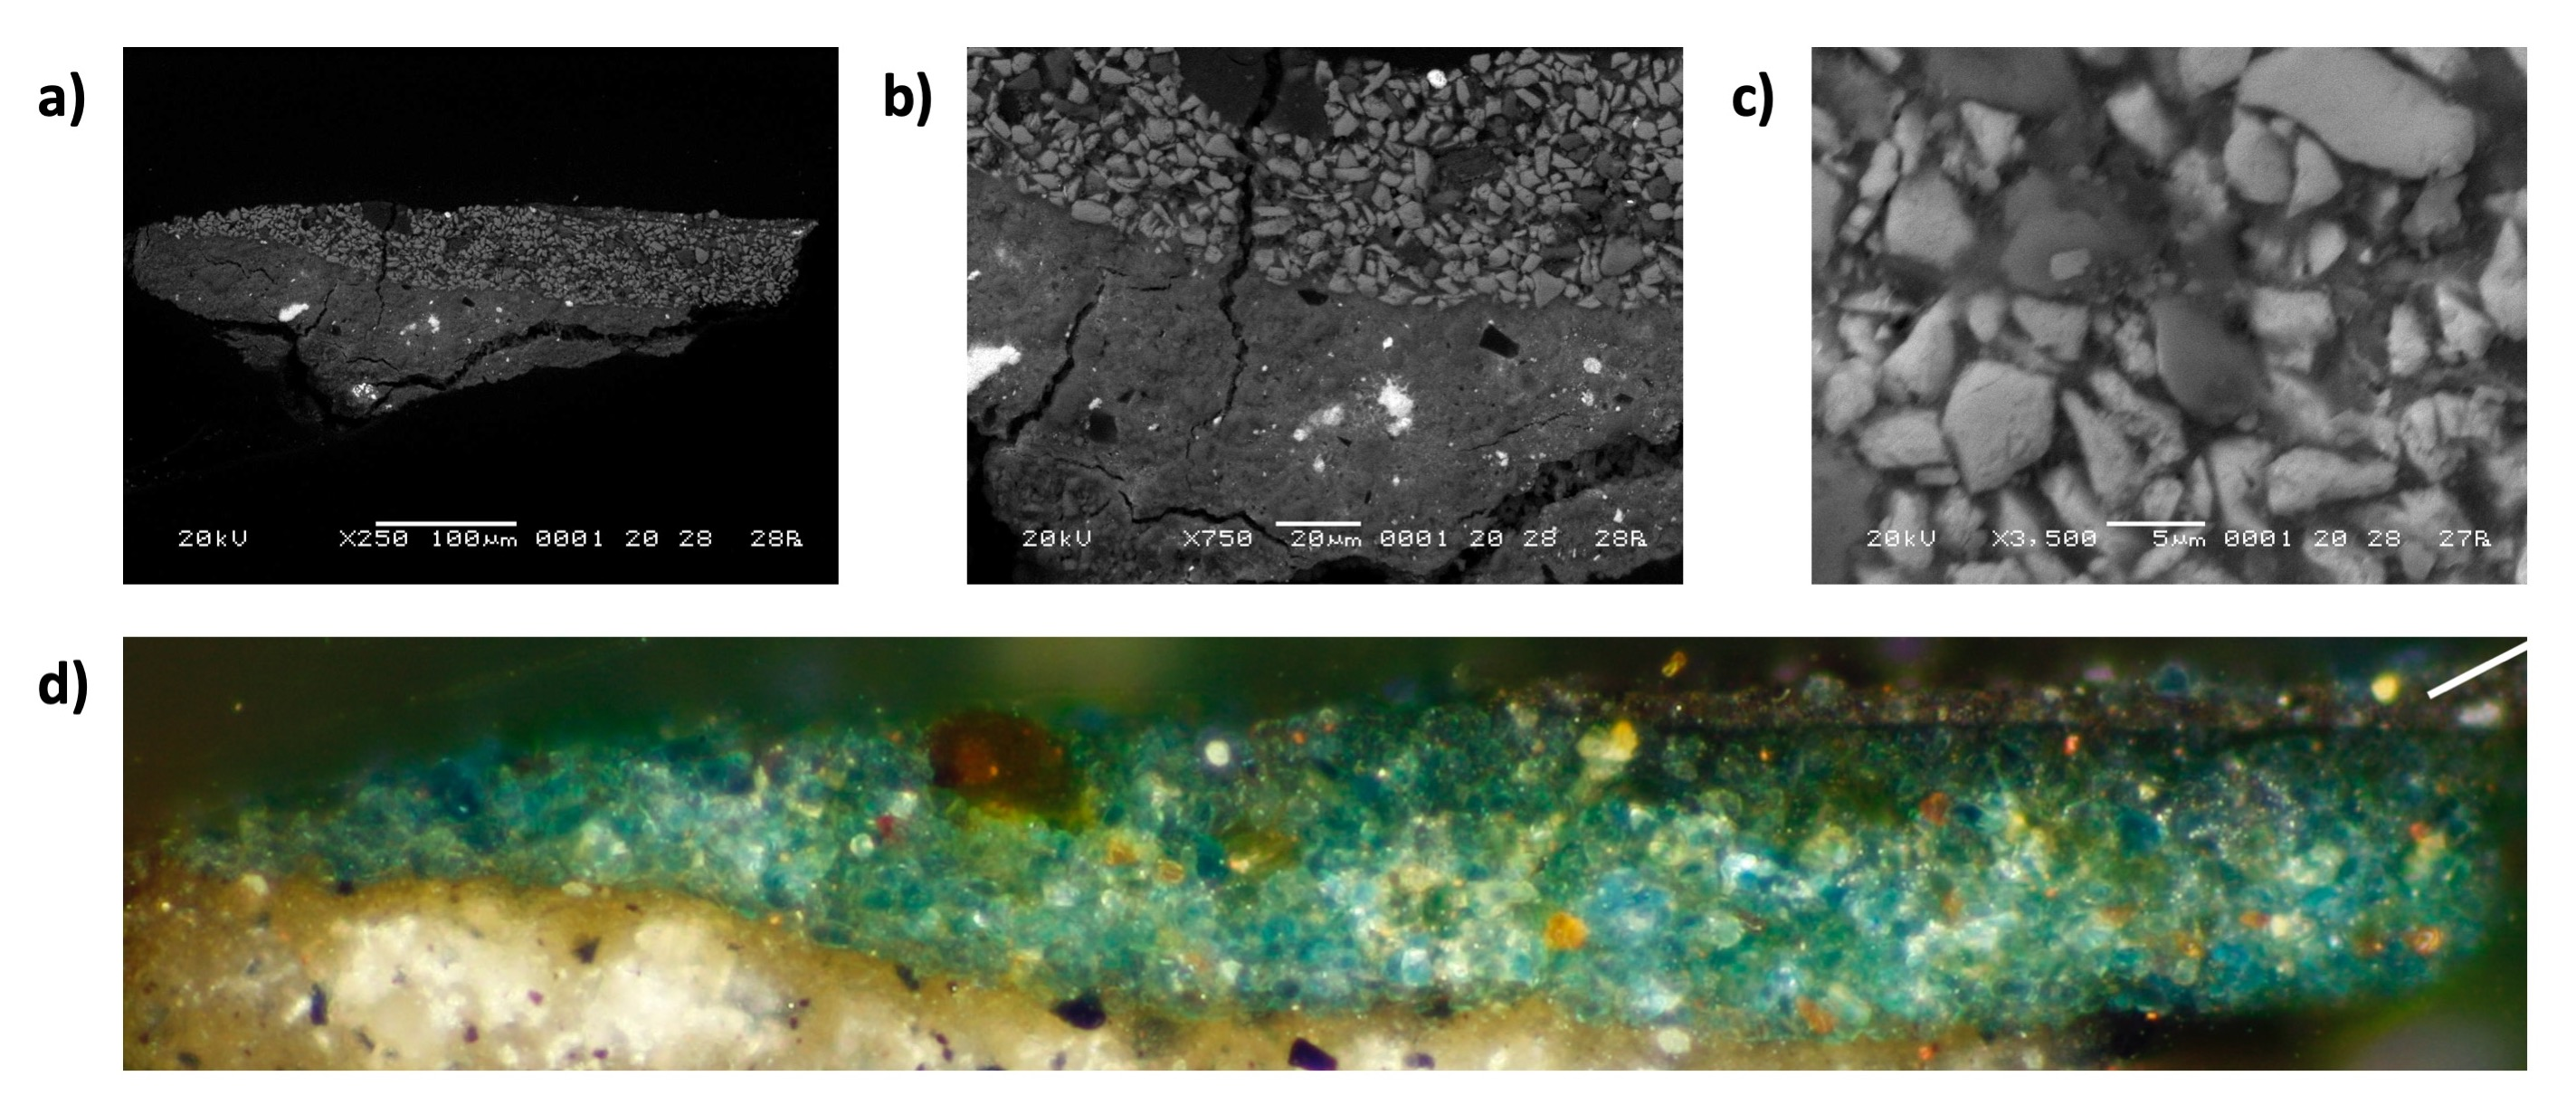
\includegraphics[width=\linewidth]{1259-1_imgs}
\caption[SEM and dark-field microscope images of sample 1259.1.]{SEM and dark-field microscope images of sample 1259.1: \textbf{a)} 250x magnification, \textbf{b)} 750x magnification, \textbf{c)} 3500x magnification, \textbf{d)} dark field microscope image provided courtesy of Katharine Waldron, HKI. Distinct copper-based pigments (blue) comprise one layer, and beneath is a thick layer of white paint. A thin layer above the blue pigment is modern overpaint.}
\label{fig:1259.1_imgs}
\end{figure}

\begin{figure}[H]
\centering
\begin{minipage}[t]{\linewidth}
  \centering
  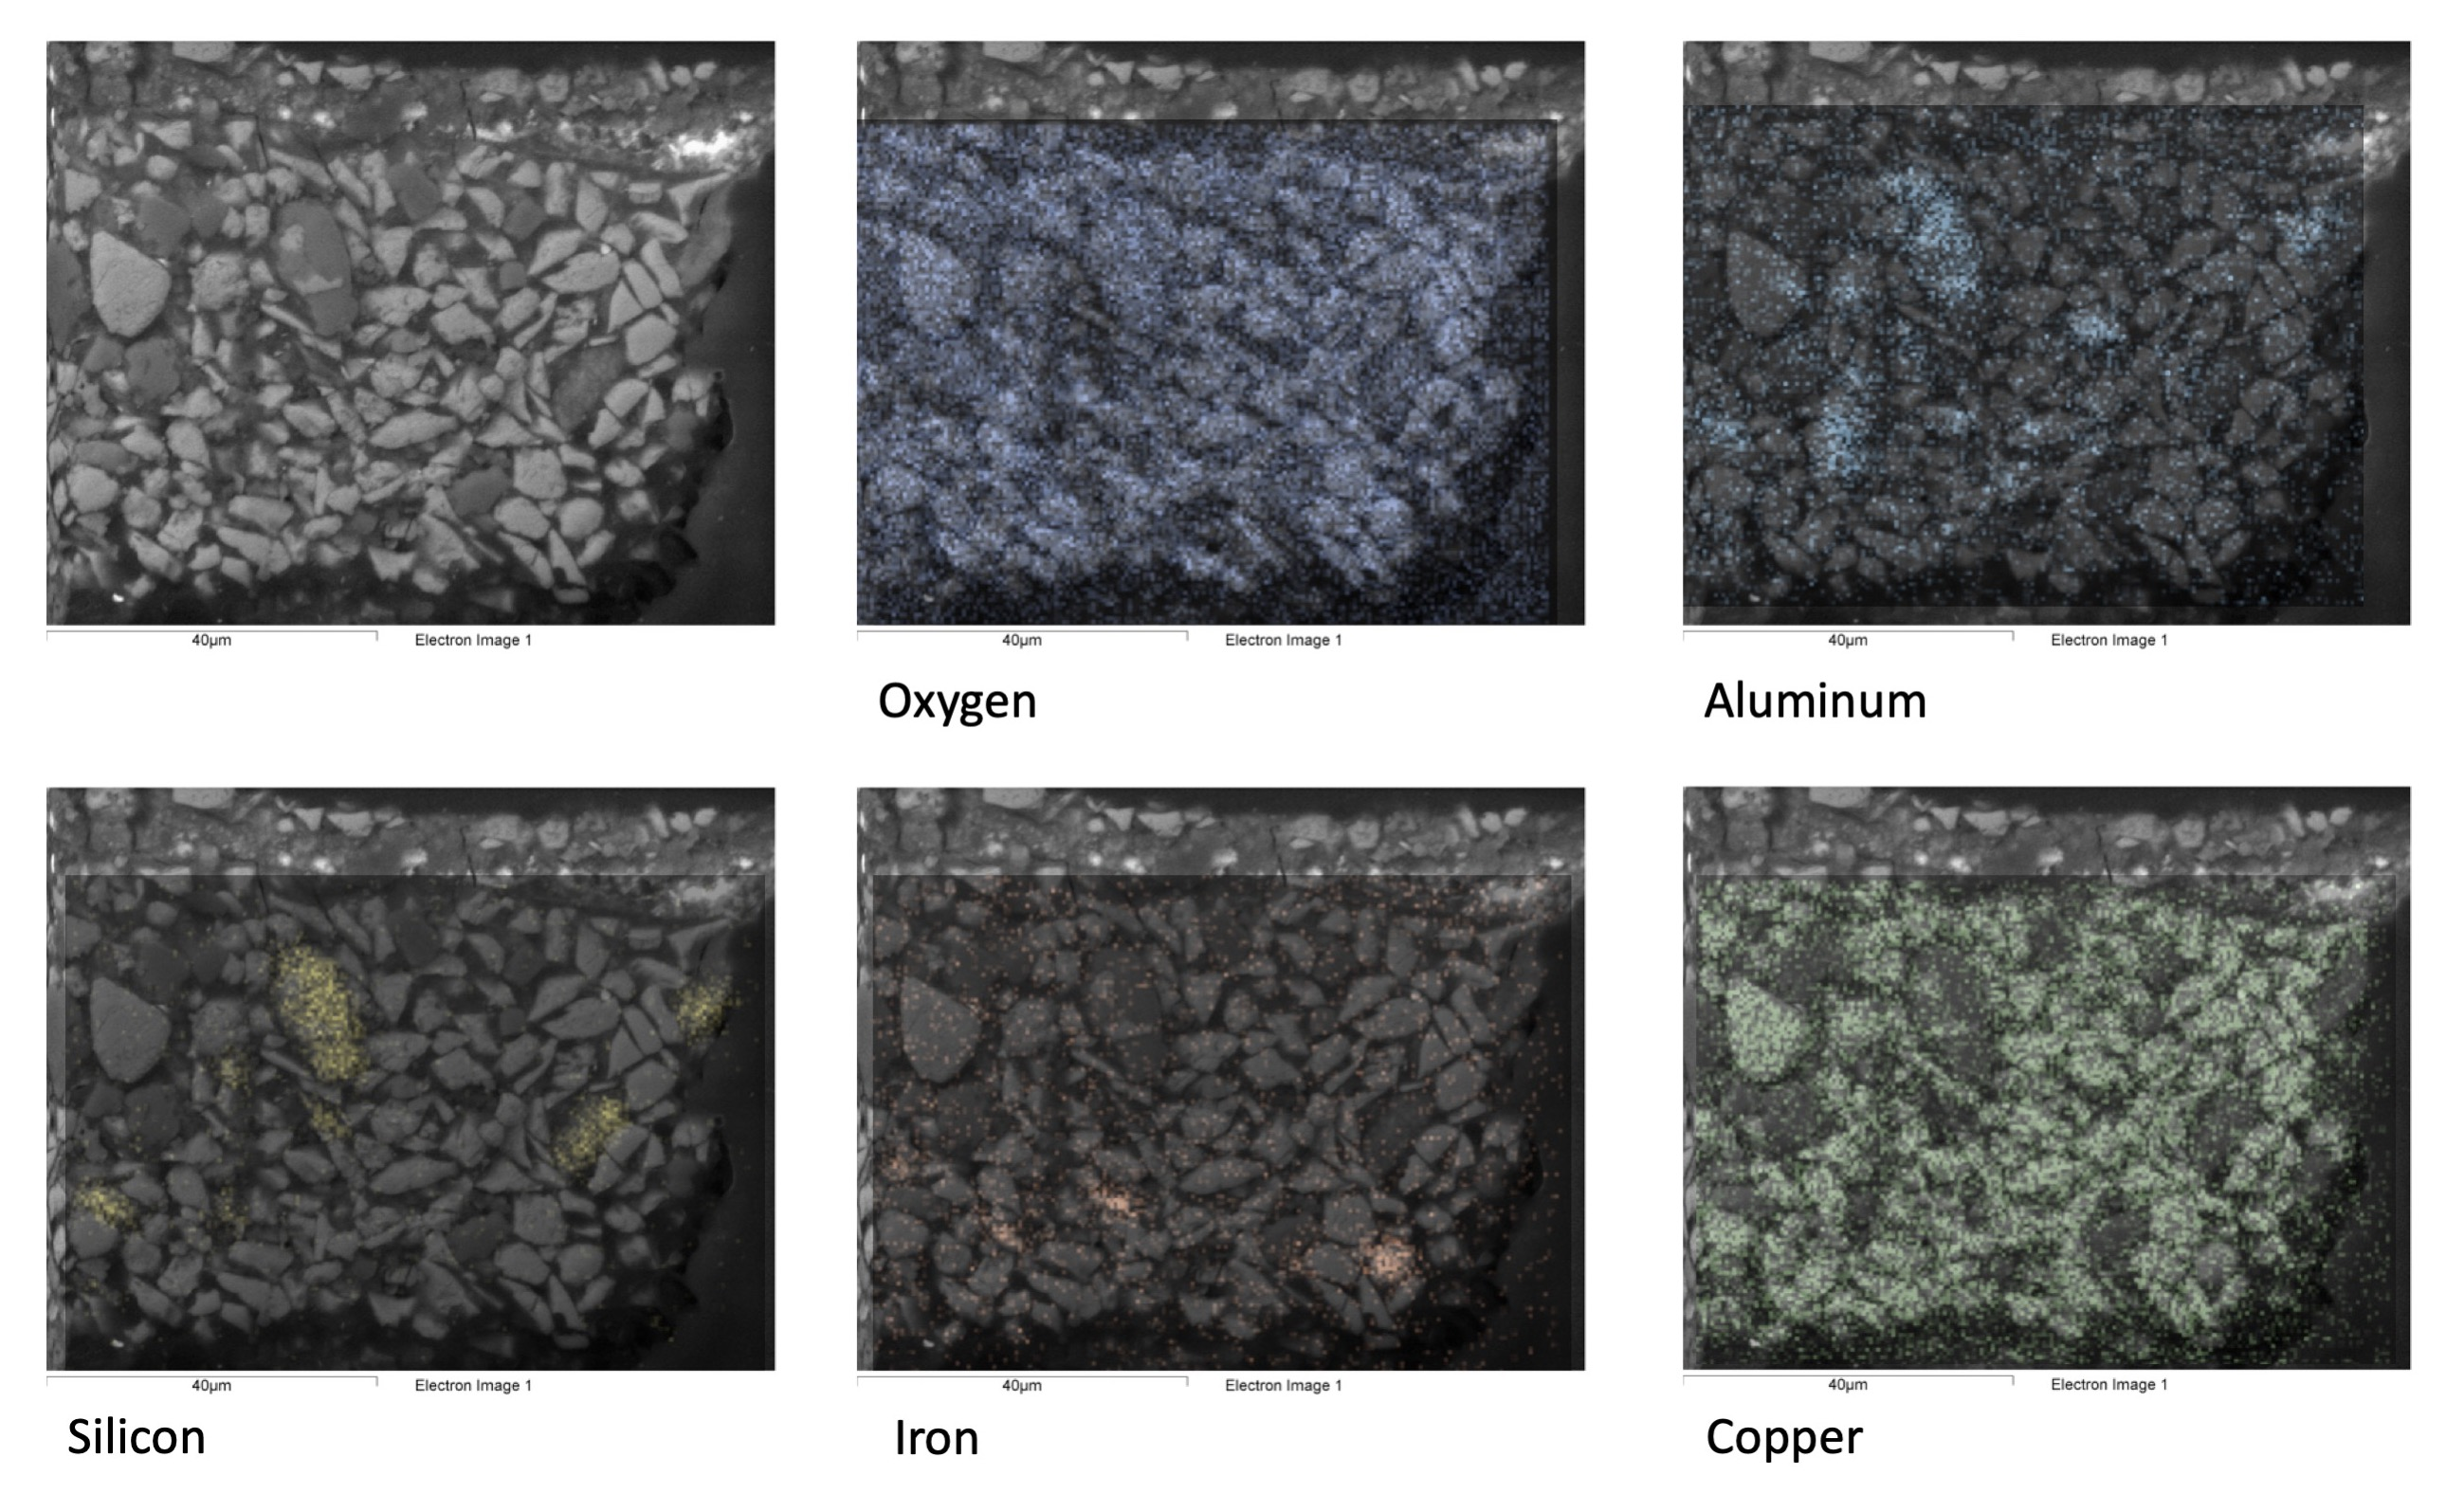
\includegraphics[width=0.9\linewidth]{1259-1_mapdata_1}
\hfill
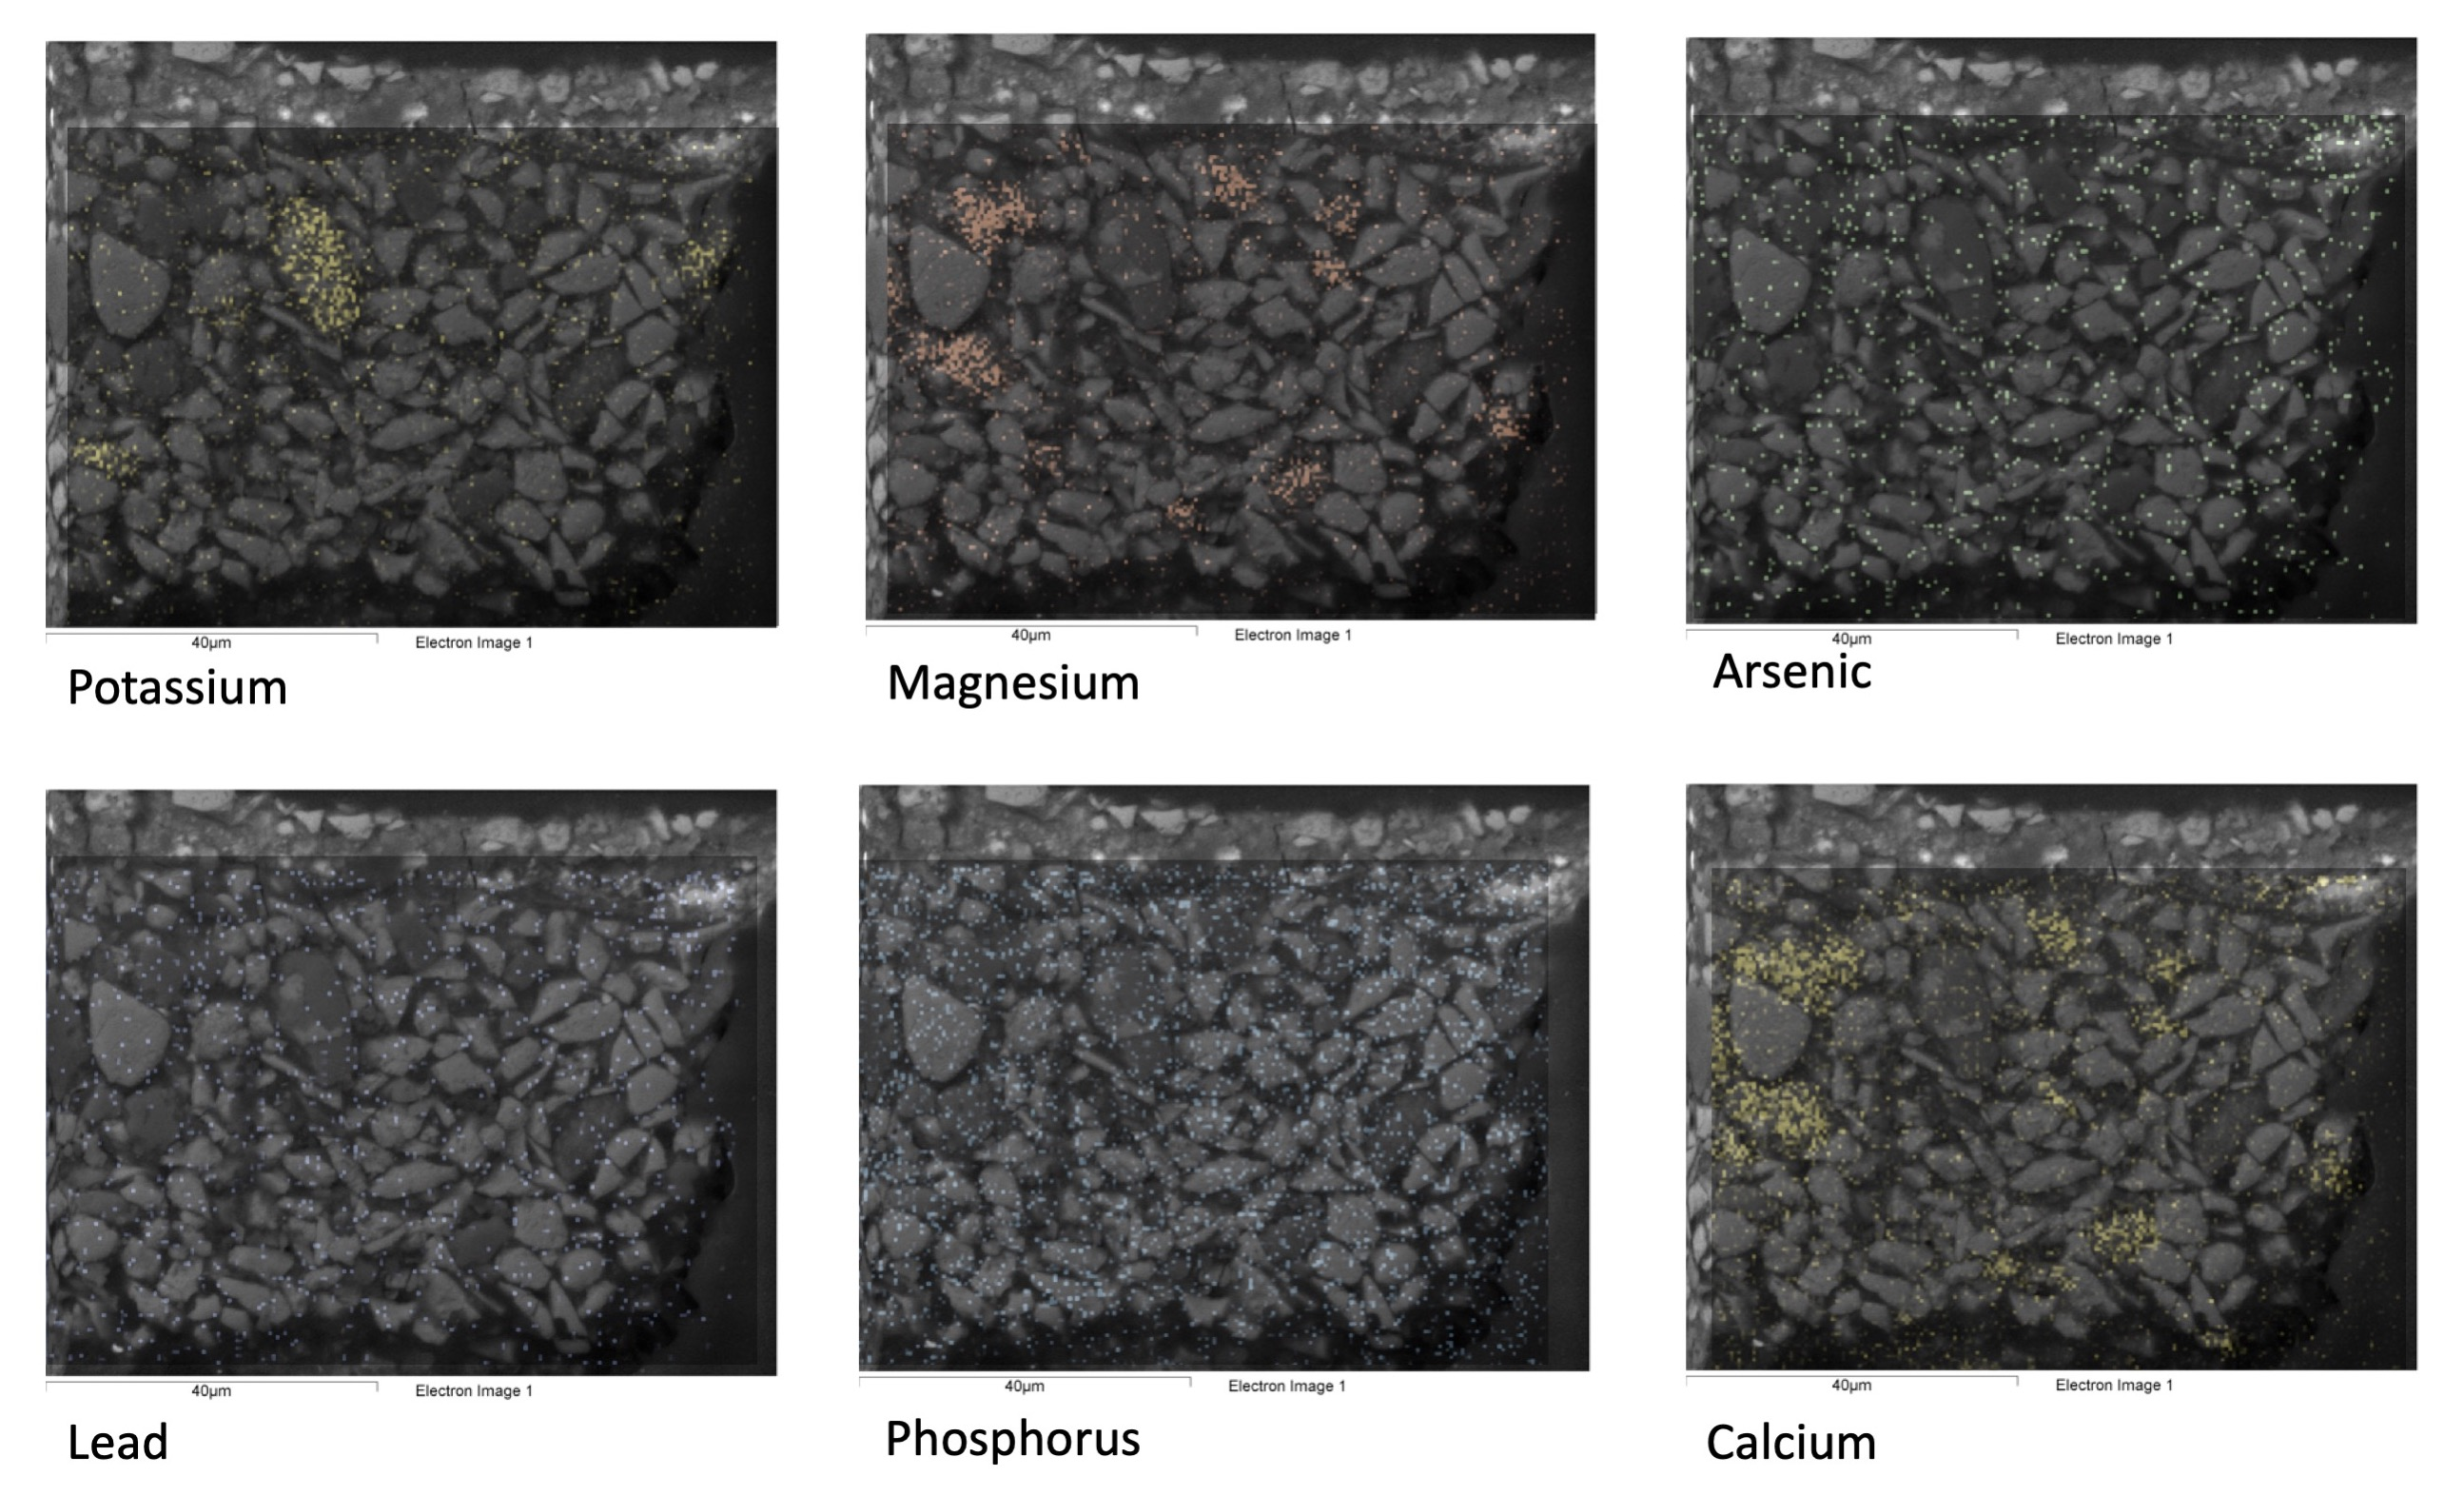
\includegraphics[width=0.9\linewidth]{1259-1_mapdata_2}
\hfill
\end{minipage}
\caption[EDS map data, sample 1259.1.]{EDS map data of sample 1259.1 showing locations of elements in an area of the azurite paint layer. Elements detected are O, Al, Si, Fe, Cu, K, Mg, As, Pb, P, and Ca.}
\label{fig:1259.1_mapdata}
\end{figure}

\begin{figure}[H]
\centering
  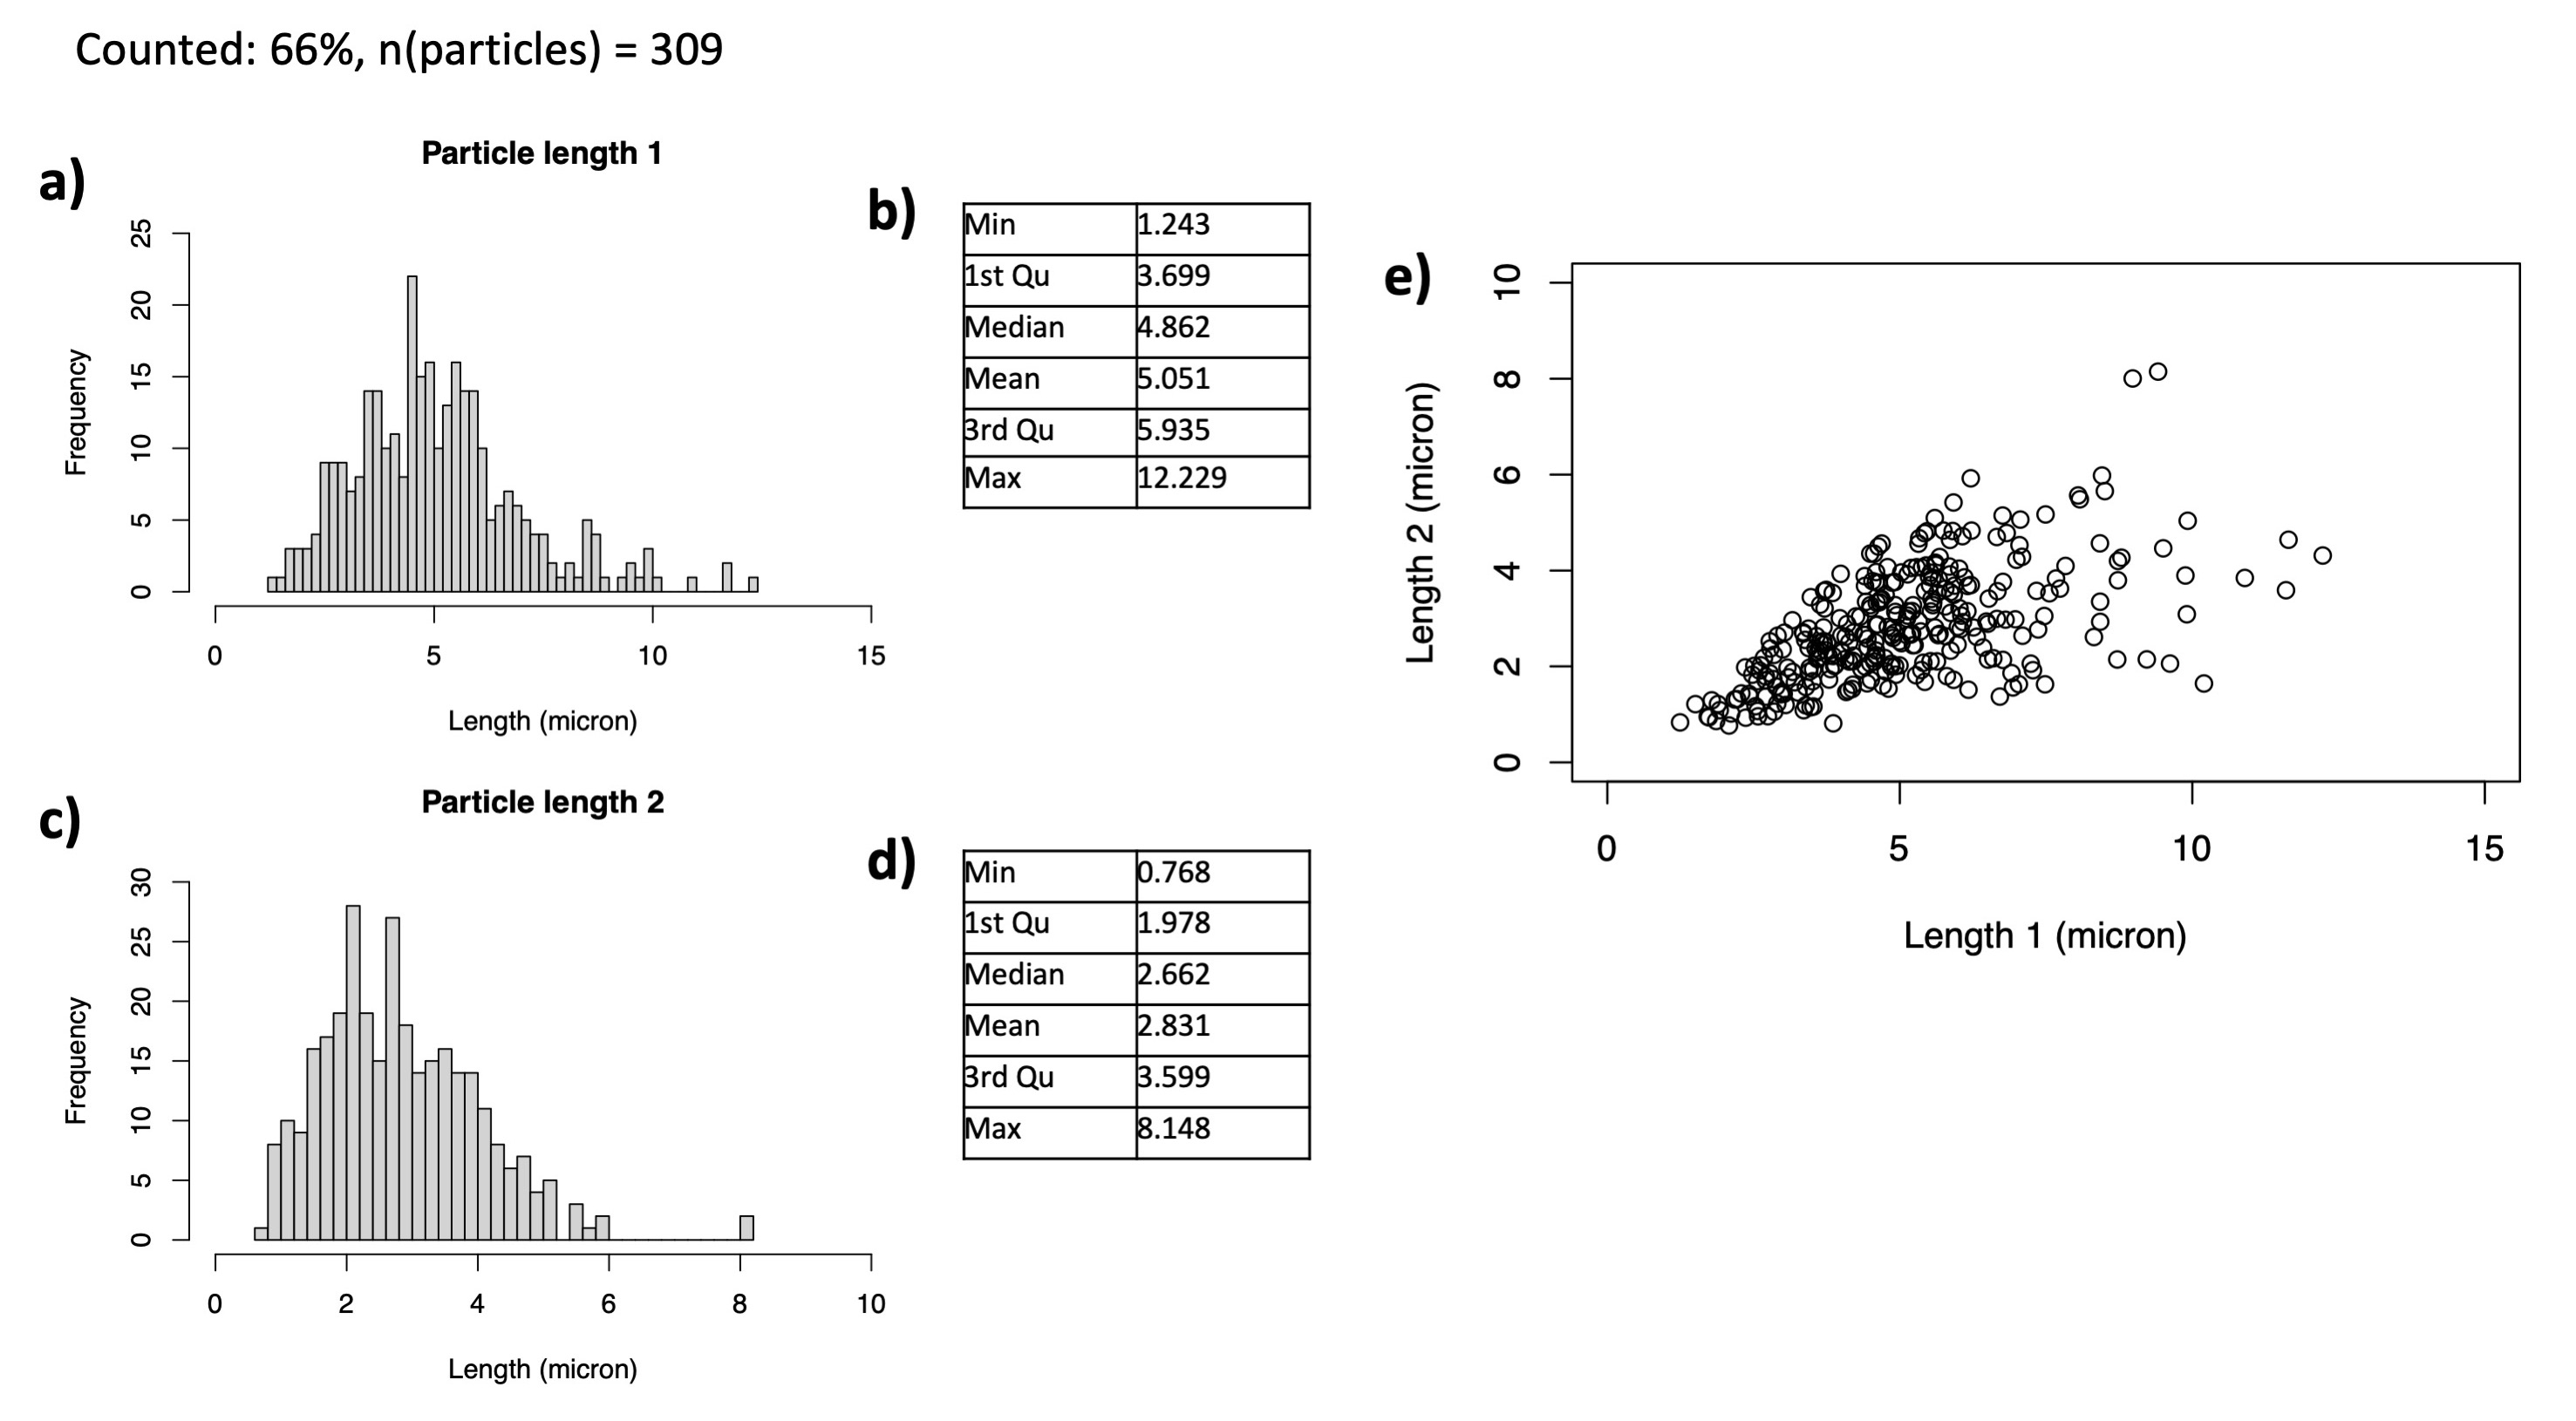
\includegraphics[width=\linewidth]{1259-1_partsize}
\caption[Particle size distribution, sample 1259.1.]{Particle size distribution of sample 1259.1: \textbf{a)} Histogram showing distribution of particle length 1 values, taken as the longest dimension. \textbf{b)} Descriptive statistics for particle length 1 data. \textbf{c)} Histogram showing distribution of particle length 2 values, taken as the longest distance perpendicular to length 1. \textbf{d)} Descriptive statistics for particle length 2 data. \textbf{e)} Graph of length 1 versus length 2 showing the degree of skew of azurite particles.}
\label{fig:1259.1_partsize}
\end{figure}




\section{Sample 1259.6}

\textit{Figure \ref{fig:1259.6_imgs}} shows SEM and dark field microscope images of 1259.6, and \textit{Figure \ref{fig:1259.6_partsize}} shows particle size data. SEM and dark field images show a heterogeneous mixture of pigments in the blue layer of the sample. The azurite particles are fairly irregular in size in dimension length 1, and consistently small in length 2. Particles are skewed rather than round. 

\begin{figure}[H]
  \centering
  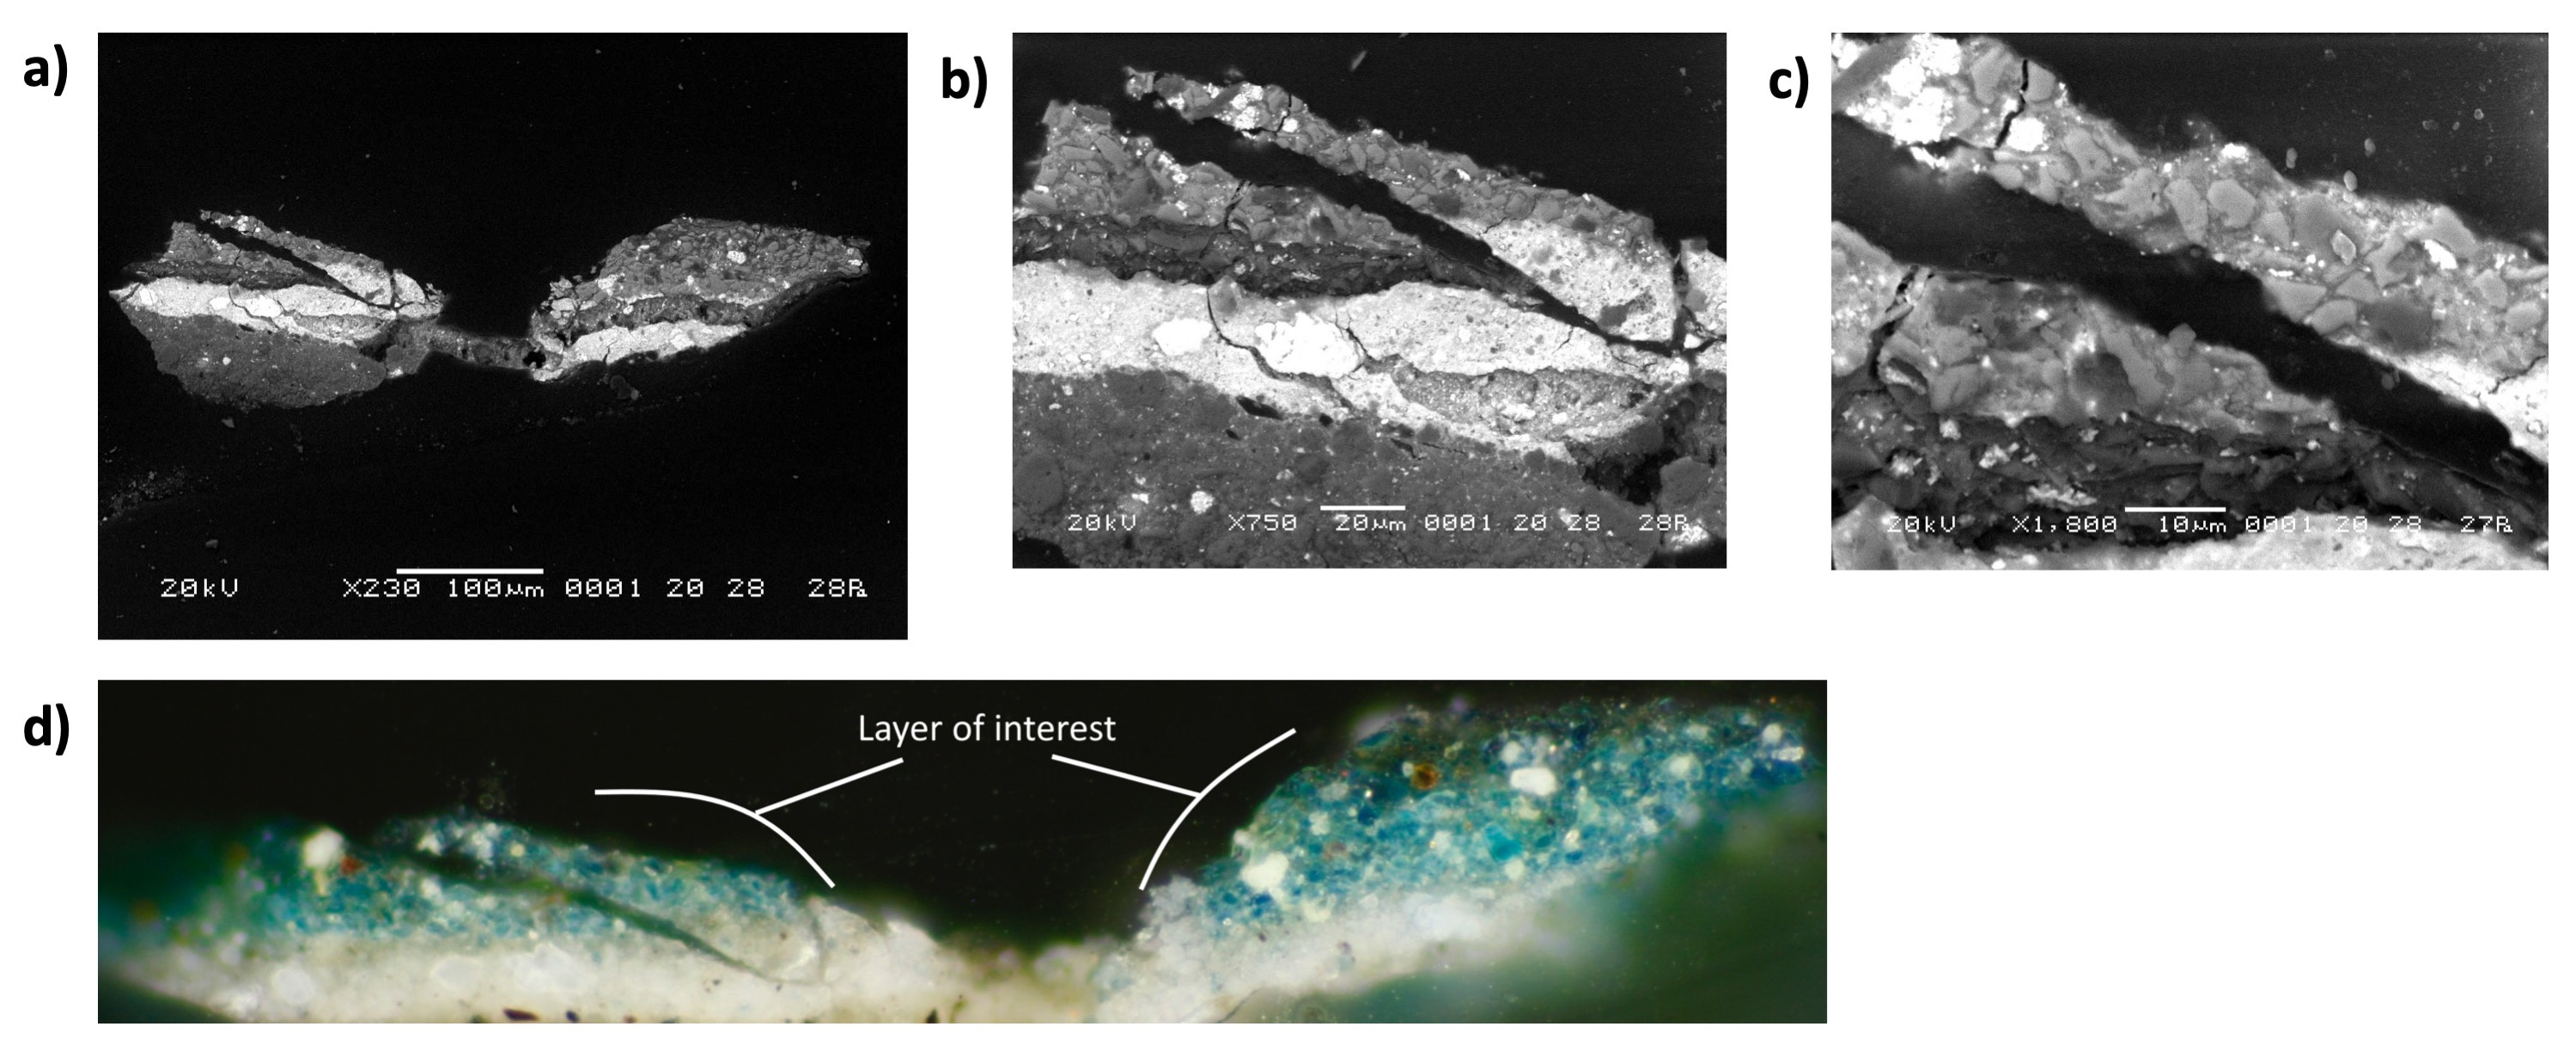
\includegraphics[width=\linewidth]{1259-6_imgs}
\caption[SEM and dark-field microscope images of sample 1259.6.]{SEM and dark-field microscope images of sample 1259.6: \textbf{a)} 230x magnification, \textbf{b)} 750x magnification, \textbf{c)} 1800x magnification, \textbf{d)} dark field microscope image provided courtesy of Katharine Waldron, HKI. A thick blue layer of azurite pigment is observed over a white base layer. The middle of the blue layer is missing.}
\label{fig:1259.6_imgs}
\end{figure}


\begin{figure}[H]
\centering
  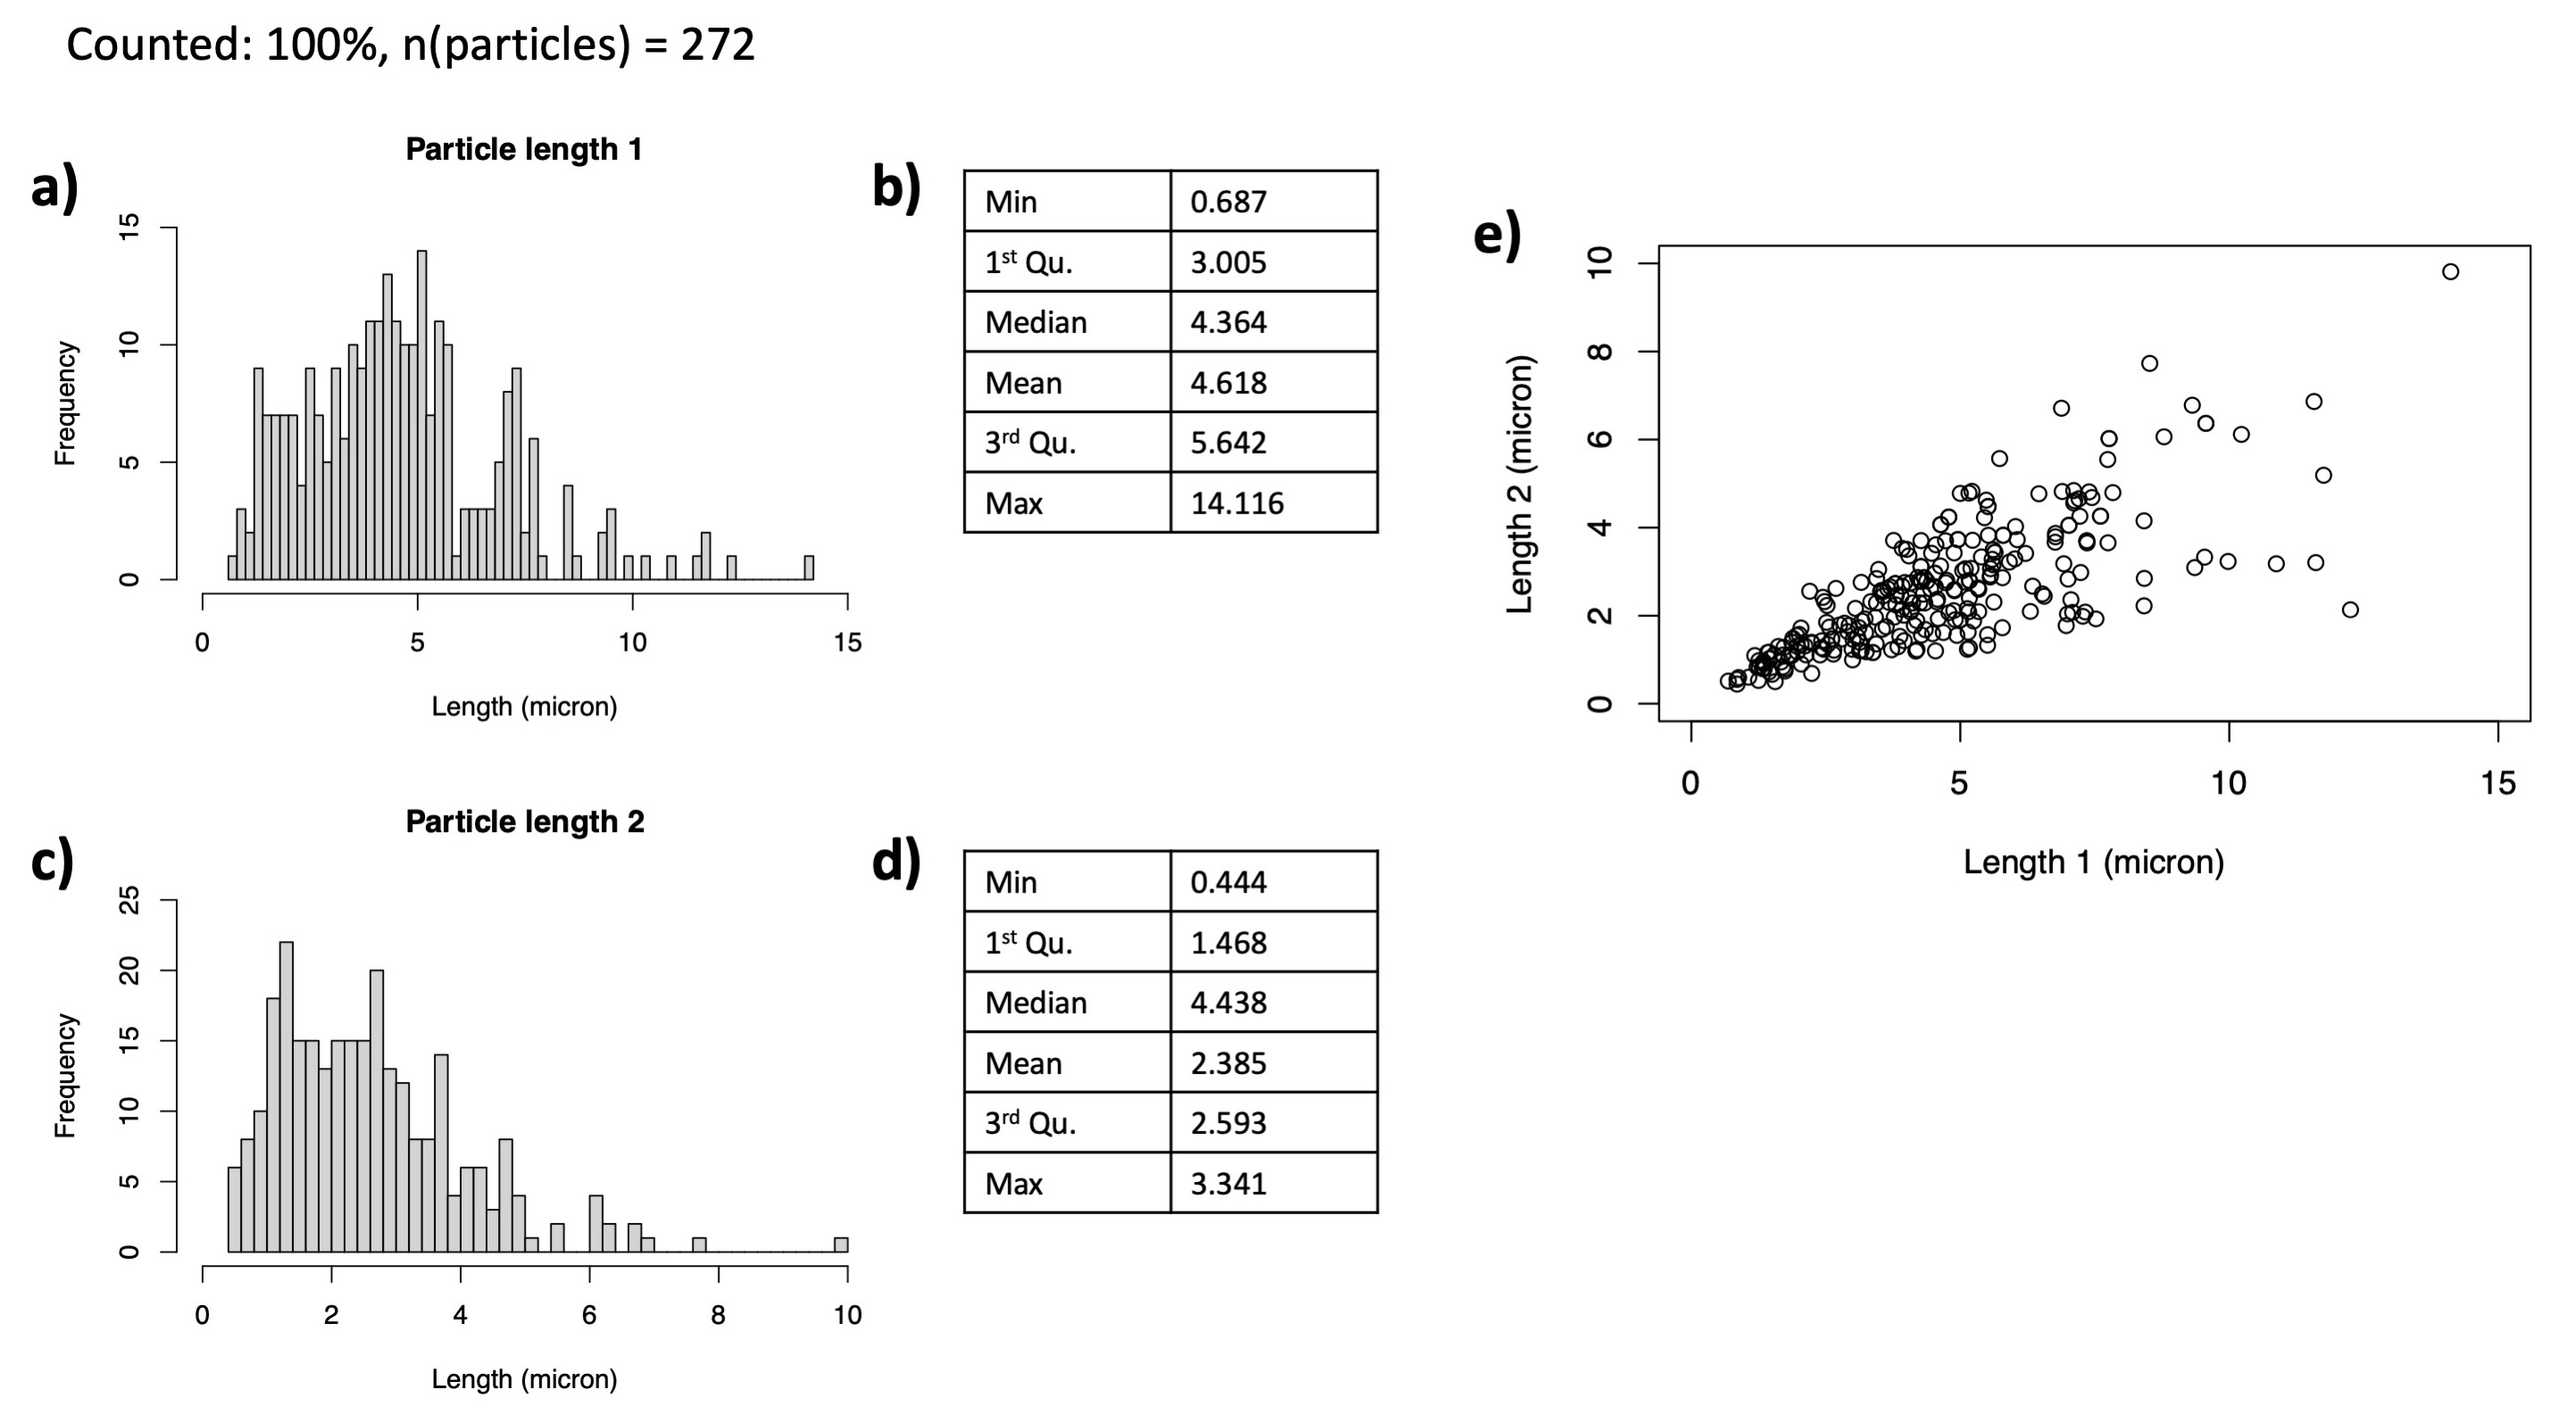
\includegraphics[width=0.9\linewidth]{1259-6_partsize}
\caption[Particle size distribution, sample 1259.6.]{Particle size distribution of sample 1259.6: \textbf{a)} Histogram showing distribution of particle length 1 values. \textbf{b)} Descriptive statistics for particle length 1 data. \textbf{c)} Histogram showing distribution of particle length 2 values. \textbf{d)} Descriptive statistics for particle length 2 data. \textbf{e)} Graph of length 1 versus length 2 showing the degree of skew.}
\label{fig:1259.6_partsize}
\end{figure}


\section{Sample 1259.14}

\textit{Figure \ref{fig:1259.14_imgs}} presents SEM and dark field images of 1259.14, showing two distinct layers of azurite on the right side of the sample. The bottom layer extends through the cross section. White and red impurities are present, and SEM data suggests relative low density of azurite particles. EDS mapping data (\textit{Figure \ref{fig:1259.14_mapdata}}) shows azurite, iron oxide, aluminium oxide, quartz, and a mineral containing silicon but not oxygen or aluminium. Lead and arsenic are not localised in the sample, and zinc is not present. 

Particle size data is presented in \textit{Figures \ref{fig:1259.14_partsize_1}} and \textit{\ref{fig:1259.14_partsize_2}} for the bottom layer alone and the top and bottom layers together. Azurite particles are not very skewed and the distribution of length 1 values is approximately normal. 

\begin{figure}[H]
  \centering
  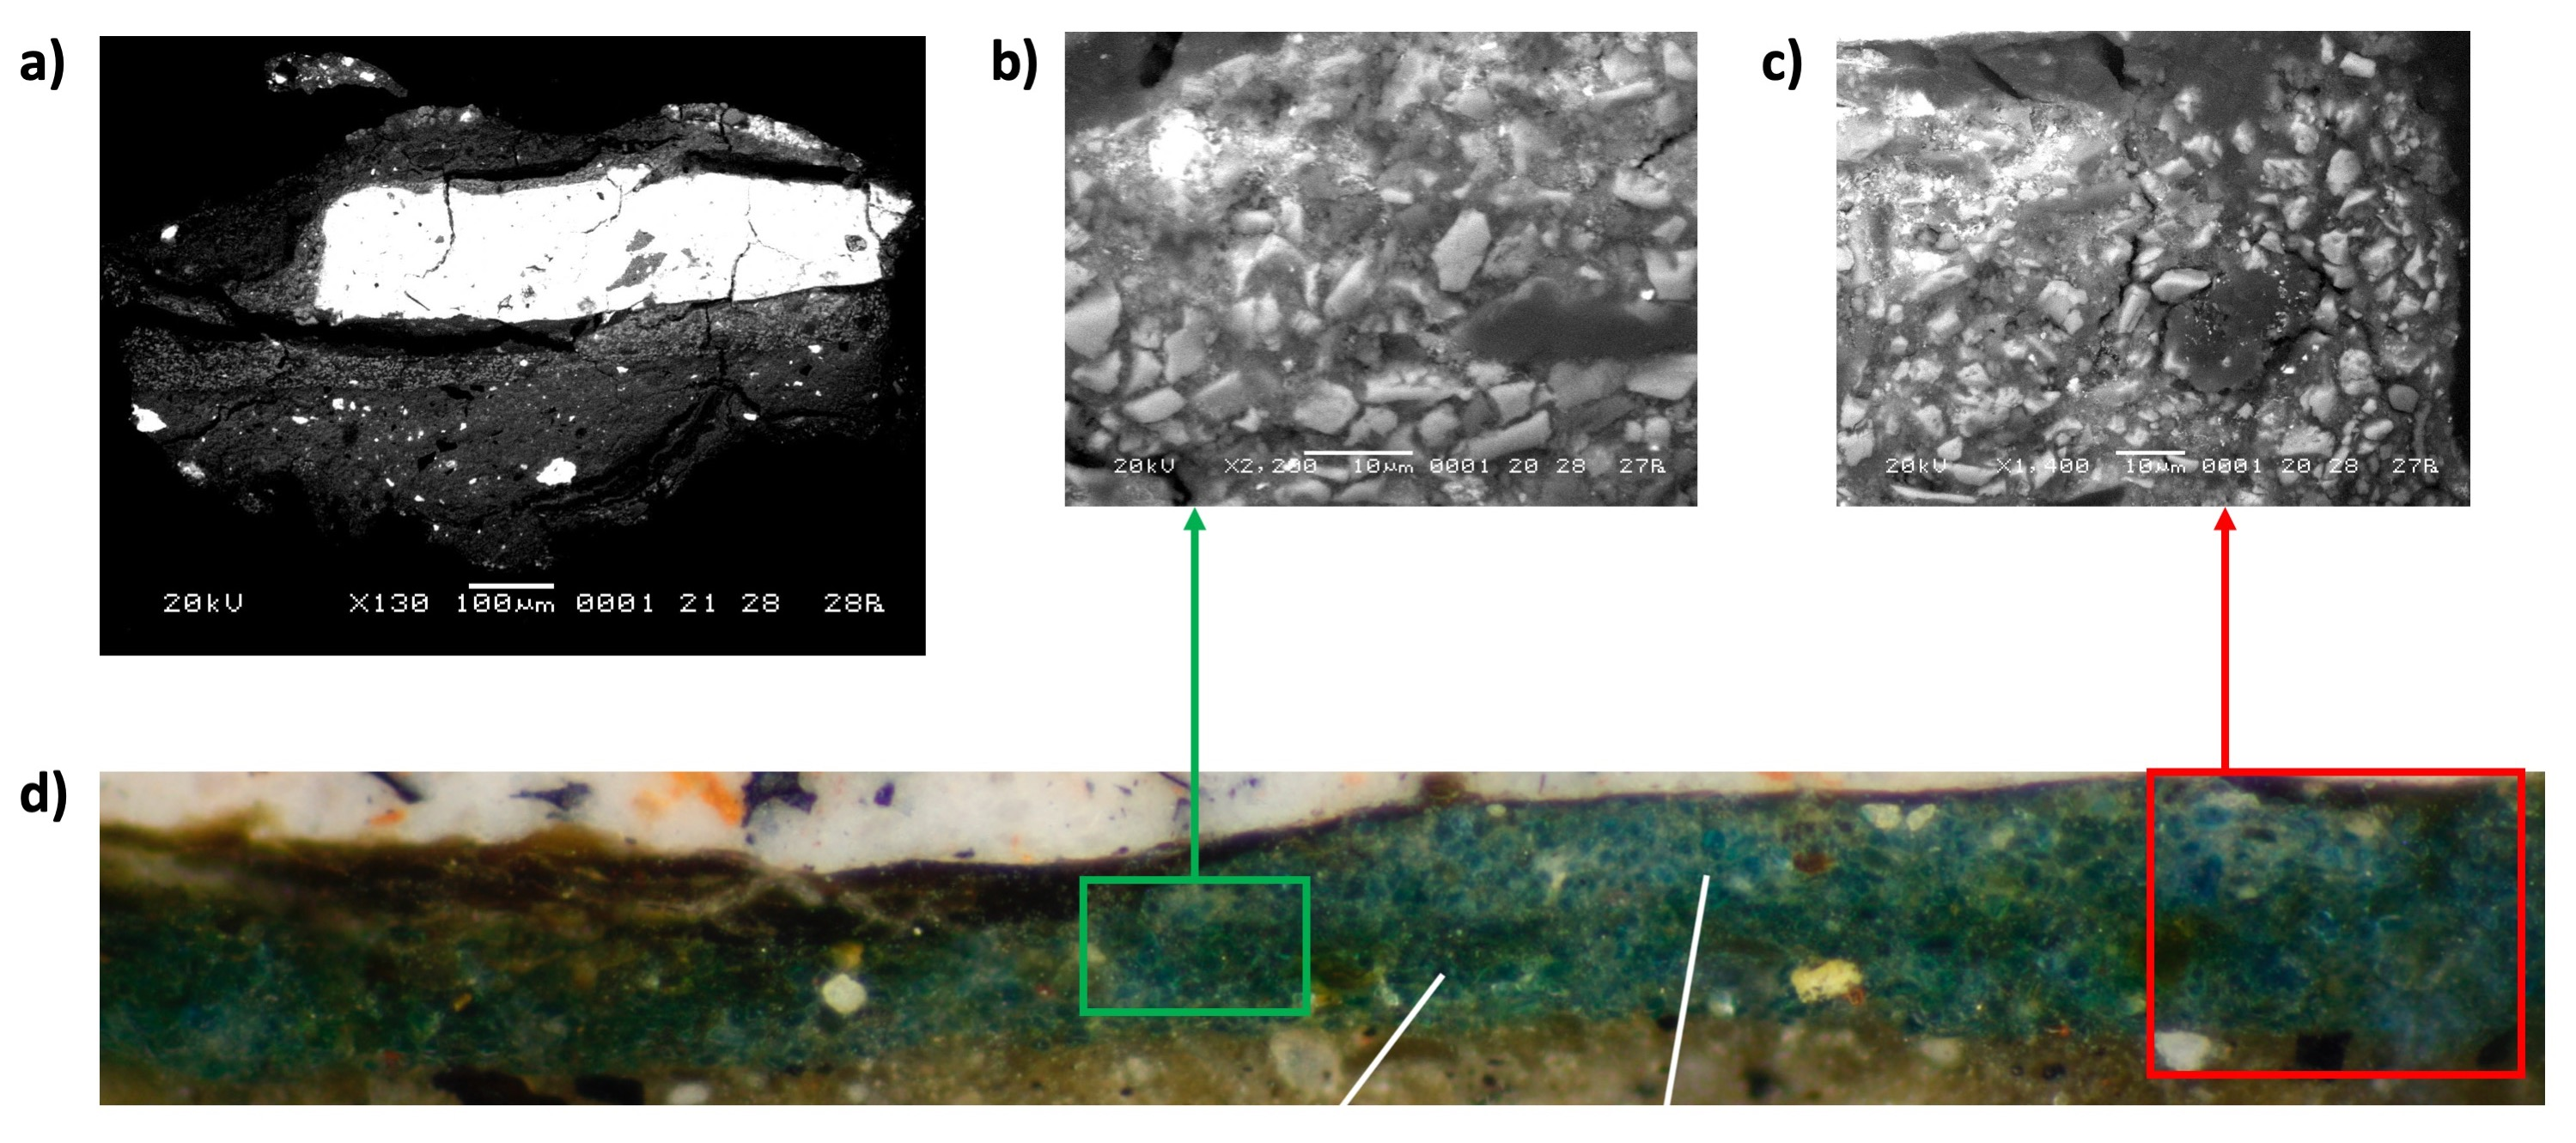
\includegraphics[width=\linewidth]{1259-14_imgs}
\caption[SEM and dark-field microscope images of sample 1259.14.]{SEM and dark-field microscope images of sample 1259.14: \textbf{a)} 130x magnification, \textbf{b)} 2200x magnification, \textbf{c)} 1400x magnification, \textbf{d)} dark field microscope image provided courtesy of Katharine Waldron, HKI. The SEM images in \textbf{b)} and \textbf{c)} show areas on the dark field image that are demarcated by green and red boxes. Two distinct layers of azurite particles are shown, the lower one extending the length of the cross section.}
\label{fig:1259.14_imgs}
\end{figure}

\begin{figure}[H]
\centering
\begin{minipage}[t]{\linewidth}
  \centering
  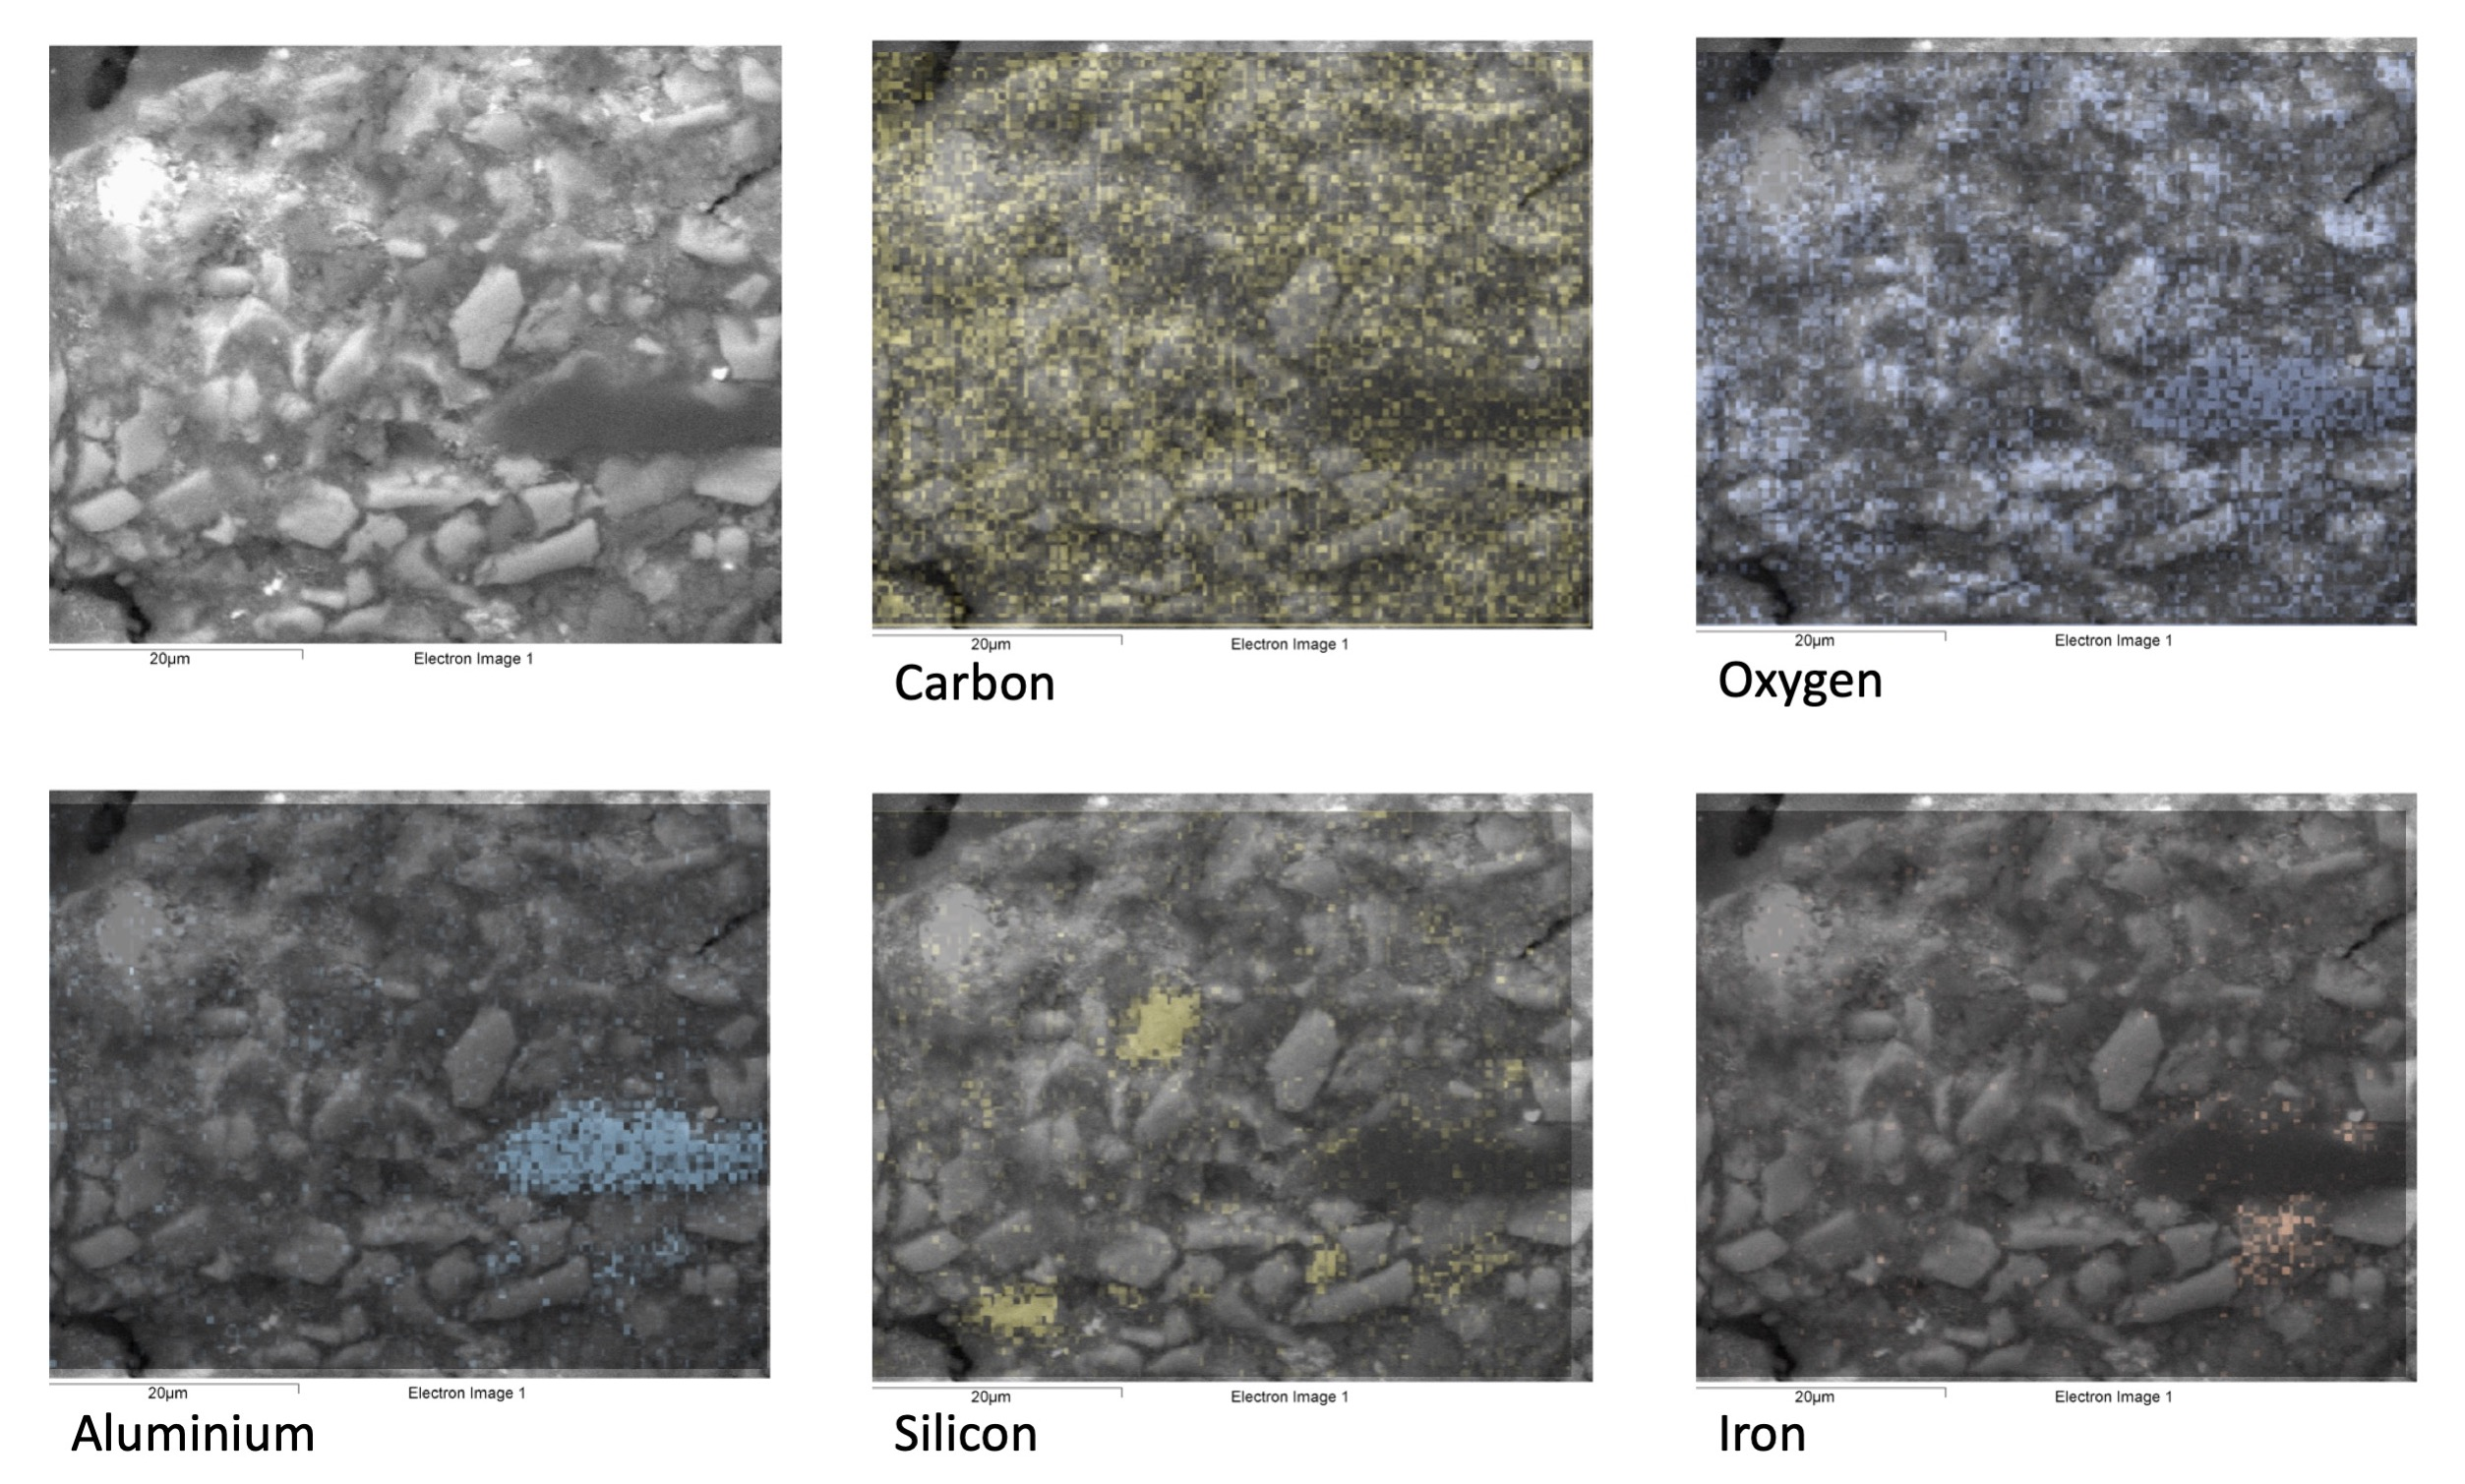
\includegraphics[width=0.9\linewidth]{1259-14_mapdata_1}
\hfill
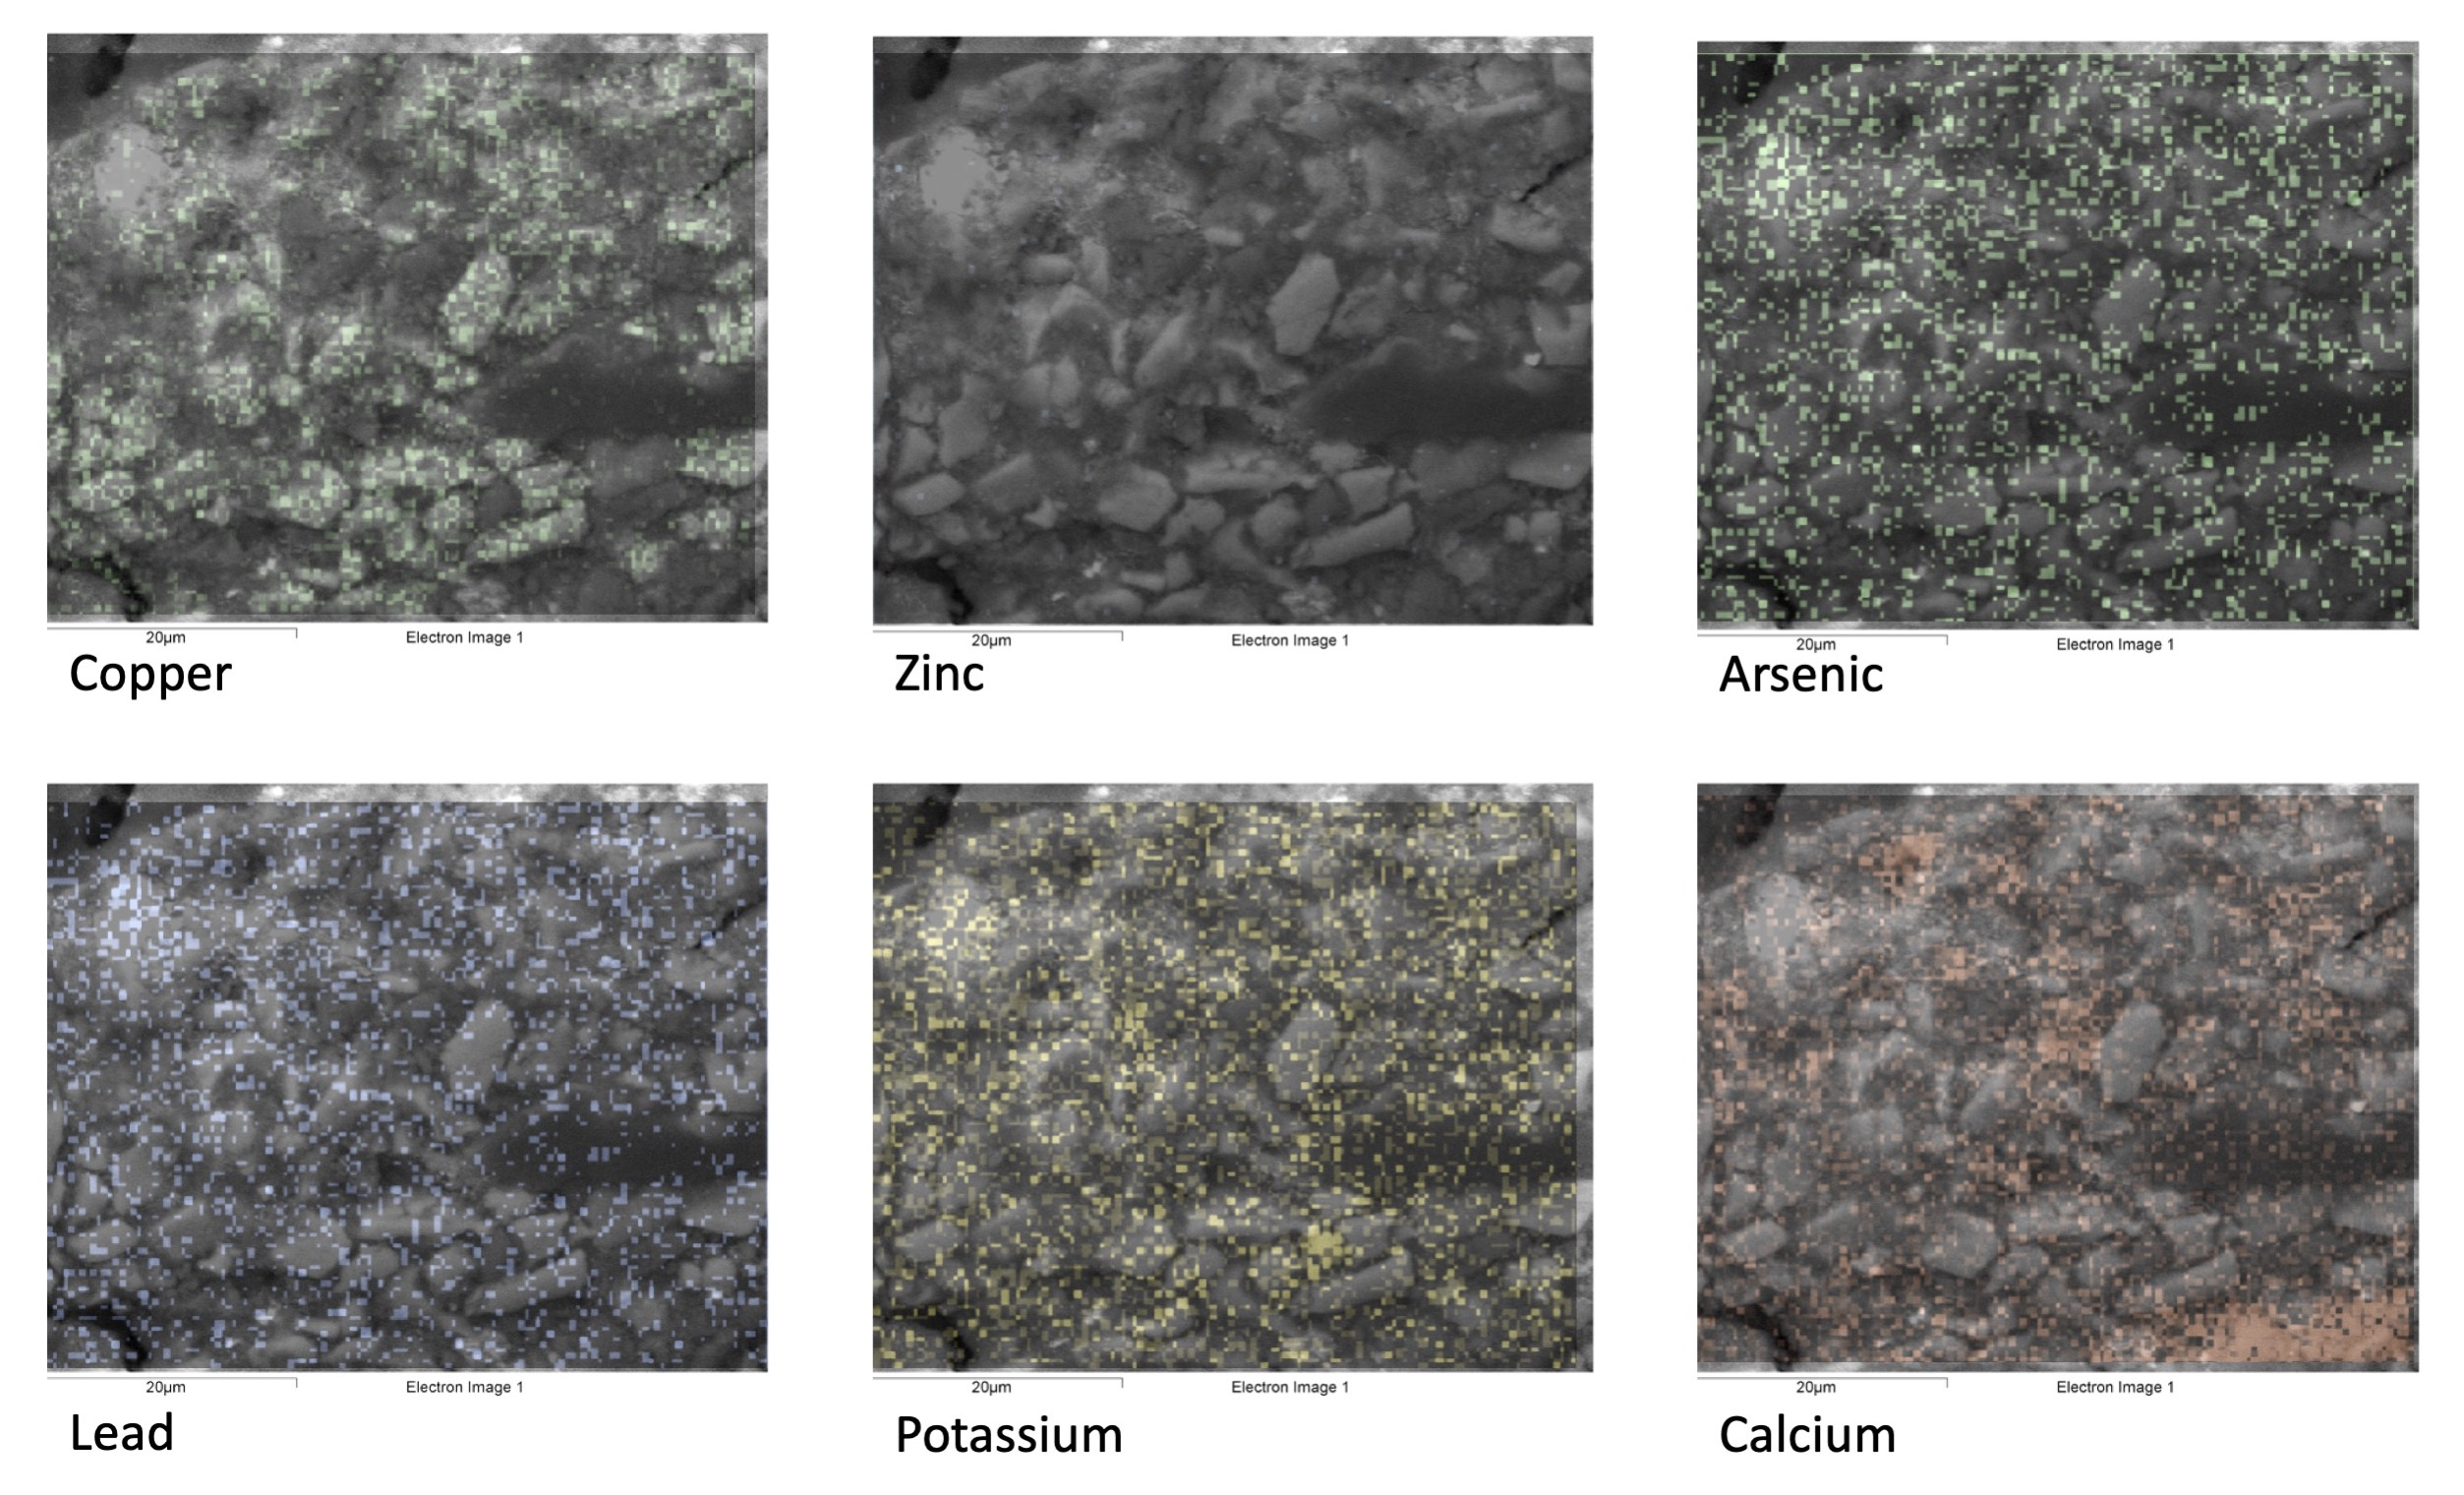
\includegraphics[width=0.9\linewidth]{1259-14_mapdata_2}
\hfill
\end{minipage}
\caption[EDS map data, sample 1259.14.]{EDS map data of sample 1259.14 showing locations of elements in an area of the azurite paint layer. Elements detected are C, O, Al, Si, Fe, Cu, Zn, As, Pb, K, and Ca.}
\label{fig:1259.14_mapdata}
\end{figure}

\begin{figure}[H]
\centering
  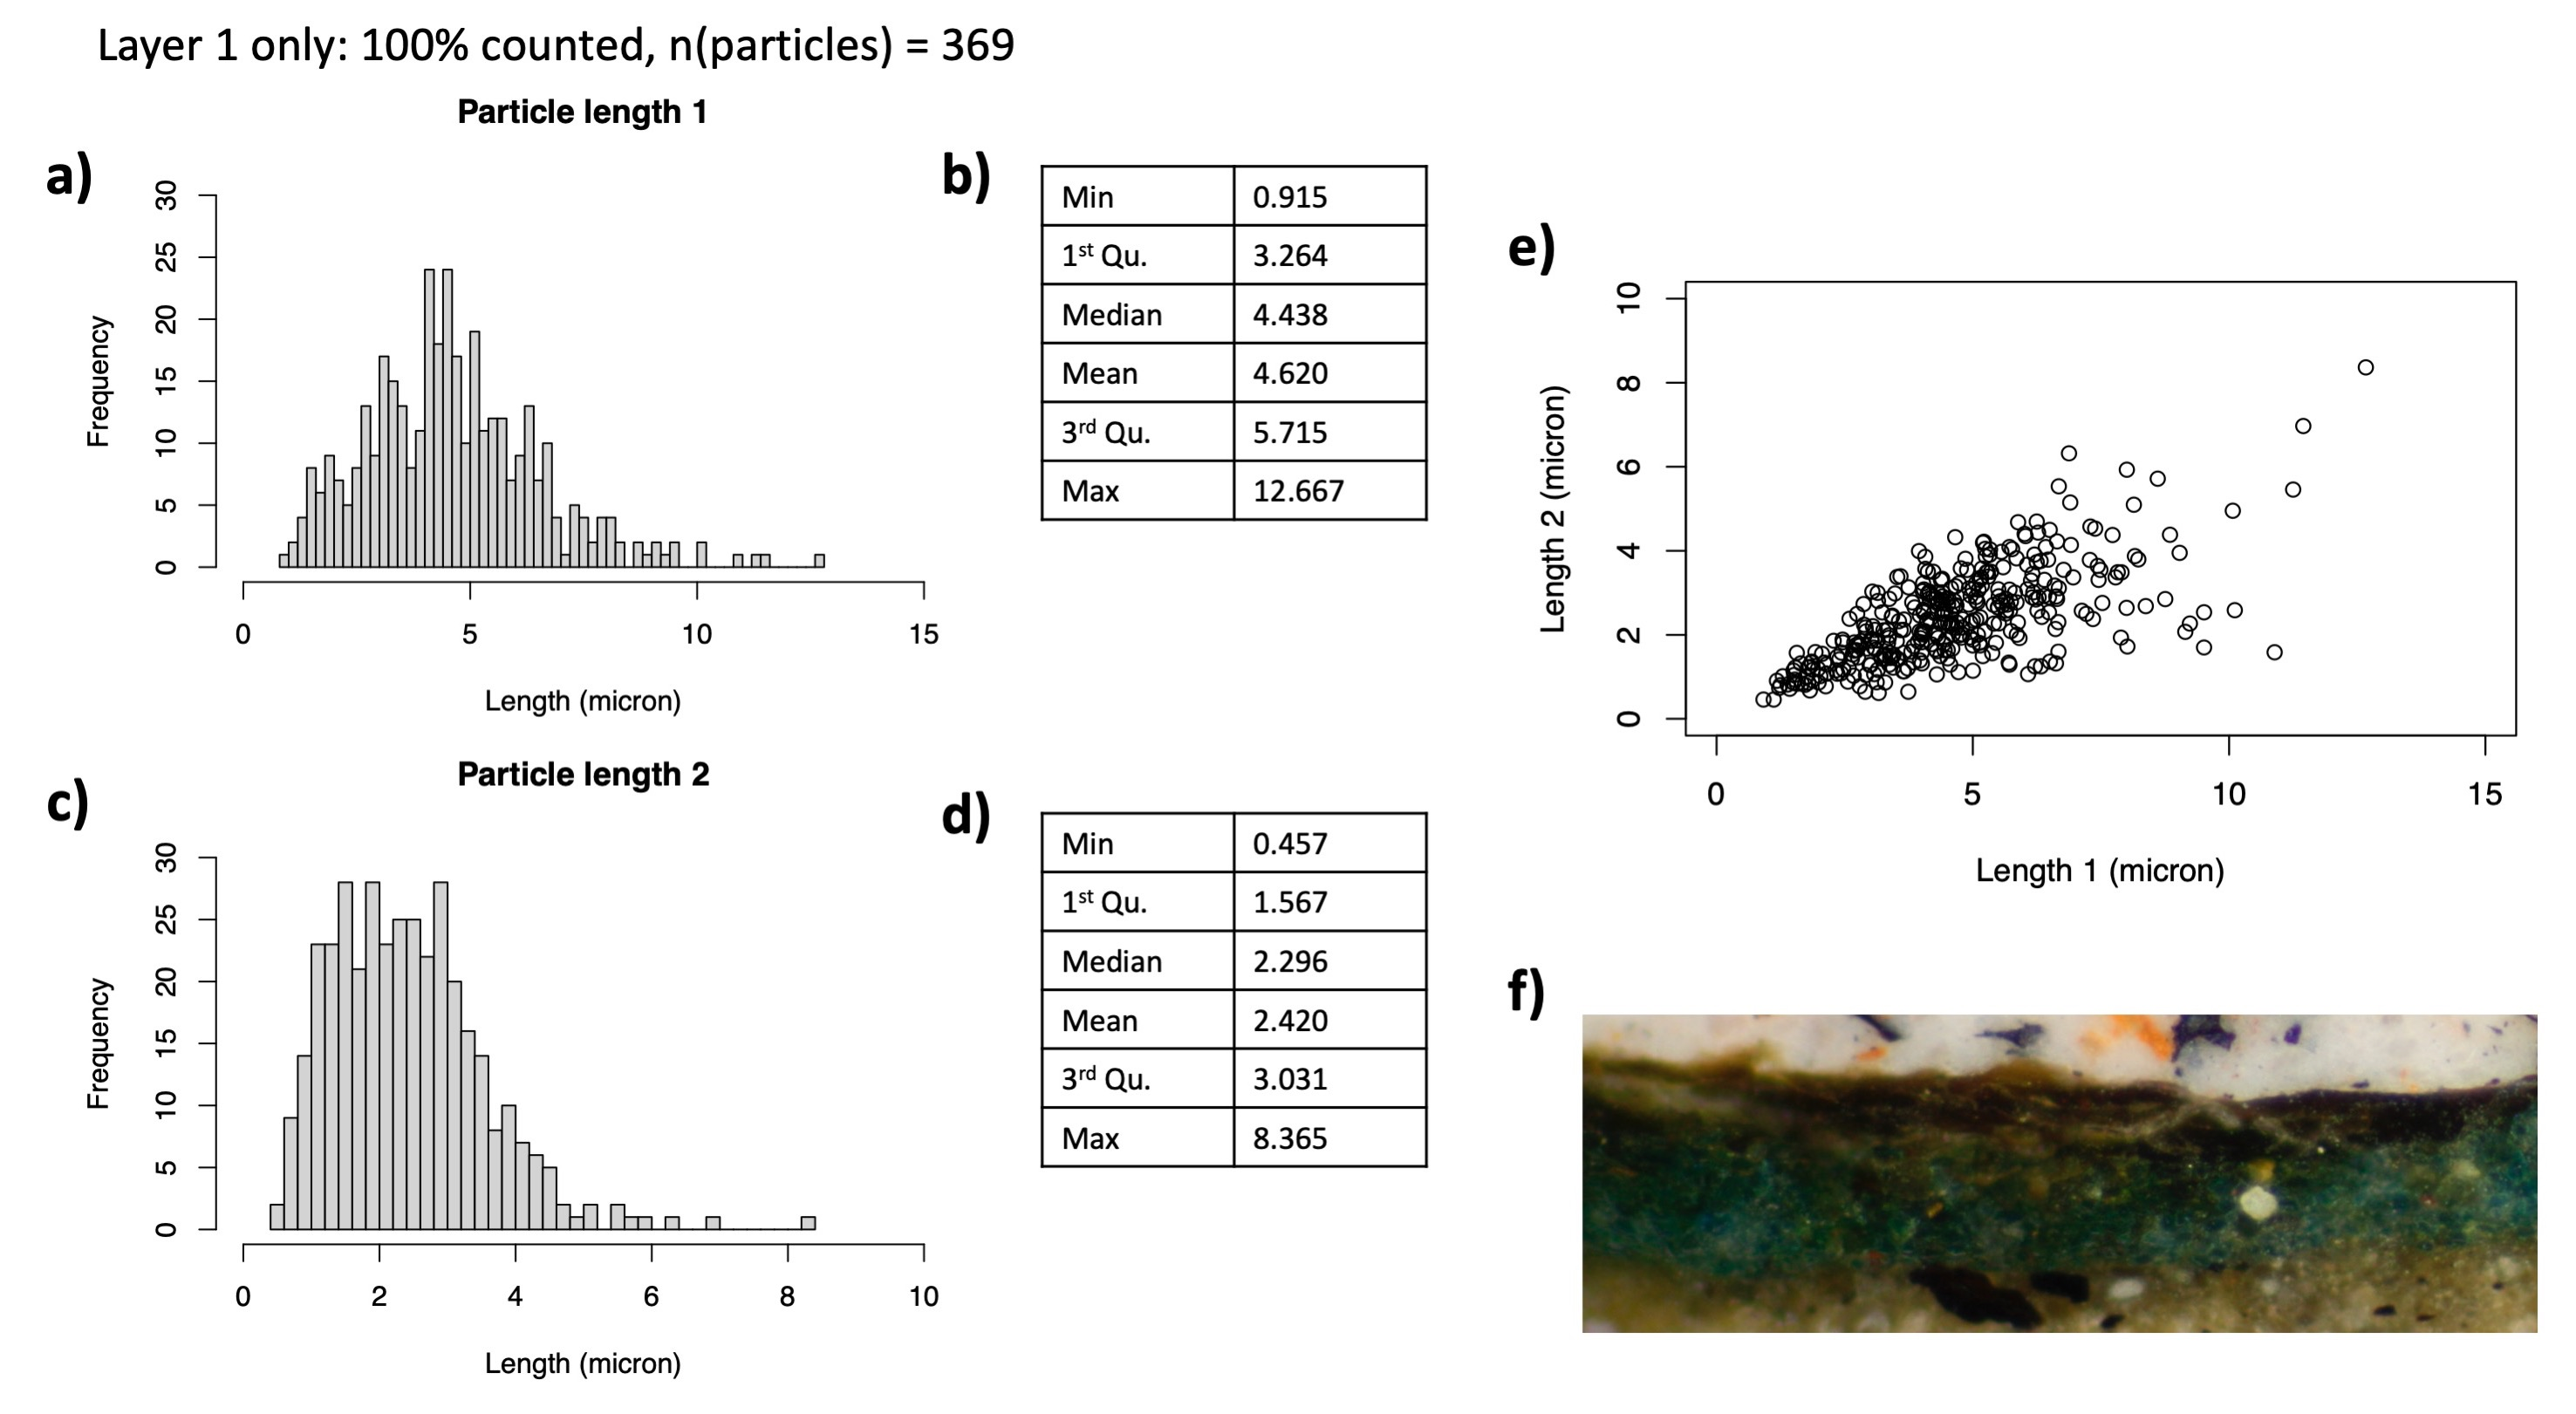
\includegraphics[width=\linewidth]{1259-14_partsize_1}
\caption[Particle size distribution, sample 1259.14 bottom layer.]{Particle size distribution of sample 1259.14, bottom layer of azurite: \textbf{a)} Histogram showing distribution of particle length 1 values. \textbf{b)} Descriptive statistics for particle length 1 data. \textbf{c)} Histogram showing distribution of particle length 2 values. \textbf{d)} Descriptive statistics for particle length 2 data. \textbf{e)} Graph of length 1 versus length 2 showing the degree of skew. \textbf{f)} Dark field microscope image (courtesy of Katharine Waldron, HKI) showing the layer in question.}
\label{fig:1259.14_partsize_1}
\end{figure}

\begin{figure}[H]
\centering
  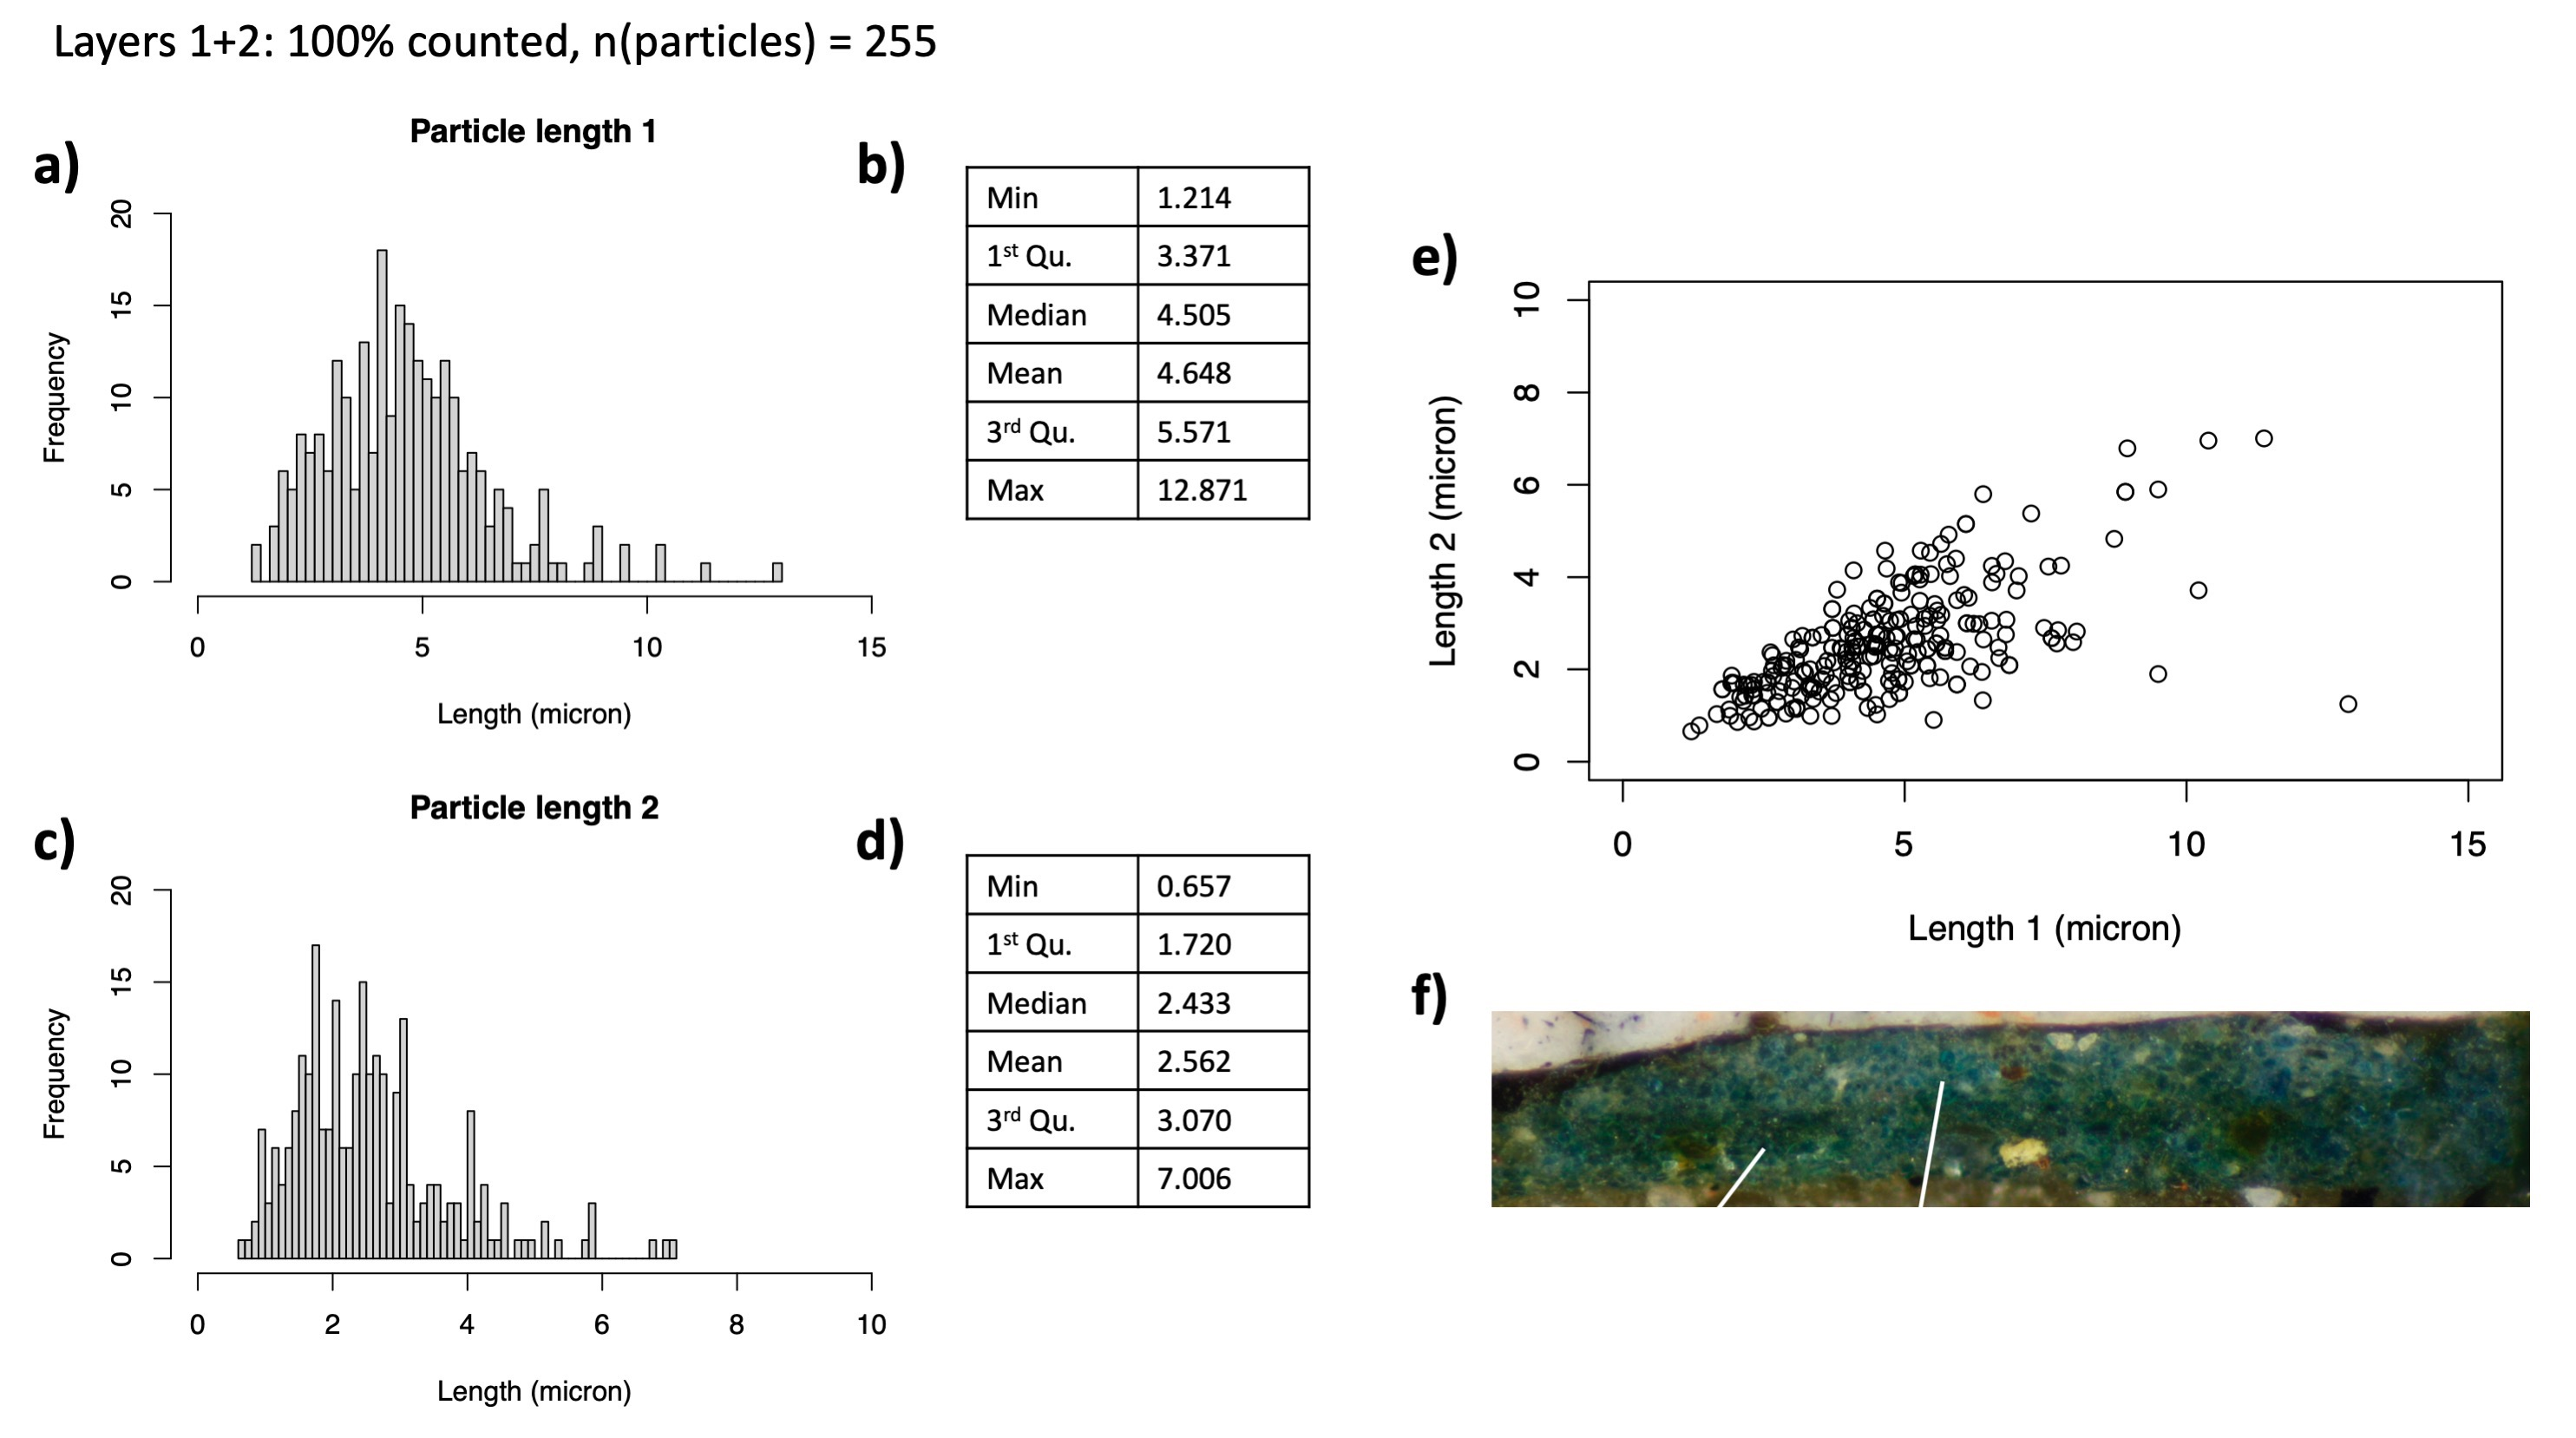
\includegraphics[width=\linewidth]{1259-14_partsize_2}
\caption[Particle size distribution, sample 1259.14 bottom and top layers.]{Particle size distribution of sample 1259.14, bottom and top layers of azurite: \textbf{a)} Histogram showing distribution of particle length 1 values. \textbf{b)} Descriptive statistics for particle length 1 data. \textbf{c)} Histogram showing distribution of particle length 2 values. \textbf{d)} Descriptive statistics for particle length 2 data. \textbf{e)} Graph of length 1 versus length 2 showing the degree of skew. \textbf{f)} Dark field microscope image (courtesy of Katharine Waldron, HKI) showing the two layers in question, marked by white lines.}
\label{fig:1259.14_partsize_2}
\end{figure}


\section{Sample 1259.19}

\textit{Figures \ref{fig:1259.19_imgs}} and \textit{\ref{fig:1259.19_partsize}} show SEM and dark field microscope images as well as particle size data for 1259.19. The thick blue paint layer of the sample is composed of azurite particles at low concentration interspersed with white pigments (likely lead white based on BES image intensity). Particle size analysis shows a majority small and round particles with several outliers showing greater skew. 


\begin{figure}[H]
  \centering
  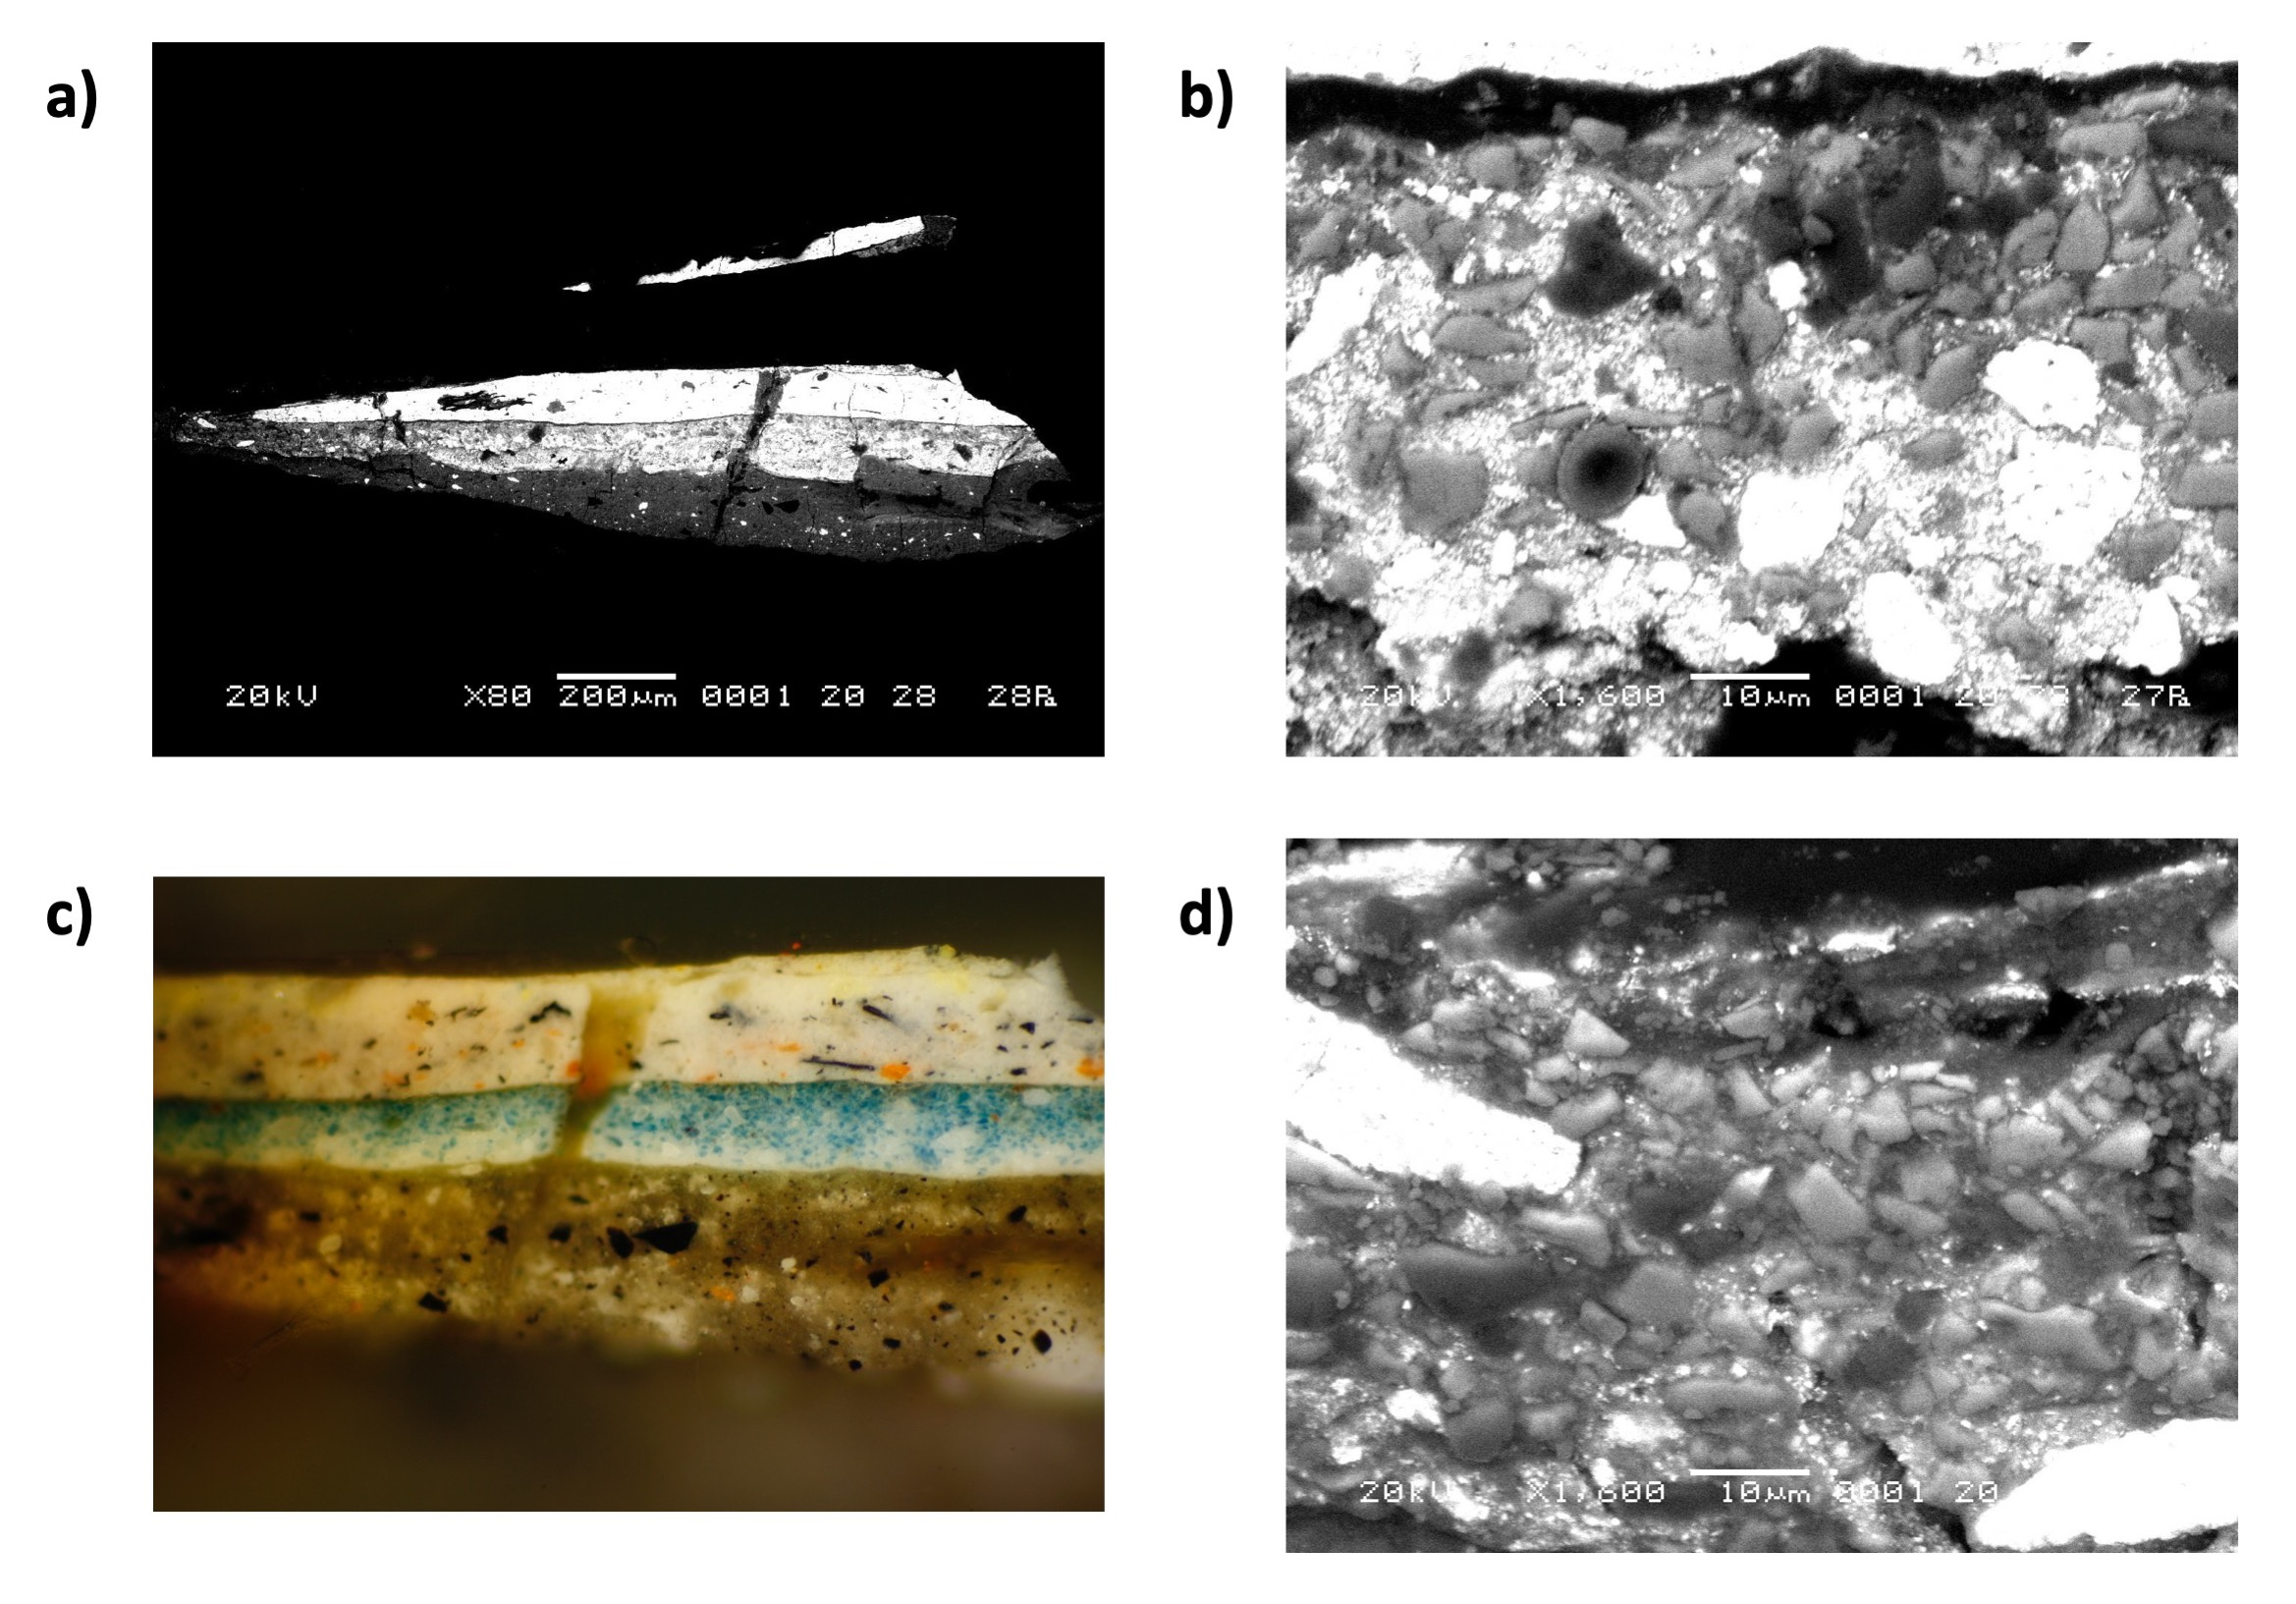
\includegraphics[width=\linewidth]{1259-19_imgs}
\caption[SEM and dark-field microscope images of sample 1259.19.]{SEM and dark-field microscope images of sample 1259.19: \textbf{a)} 80x magnification, \textbf{b)} 1600x magnification, \textbf{c)} dark field microscope image provided courtesy of Katharine Waldron, HKI, \textbf{d)} 1600x magnification. The azurite containing layer shows blue and white pigments mixed together.}
\label{fig:1259.19_imgs}
\end{figure}

\begin{figure}[H]
\centering
  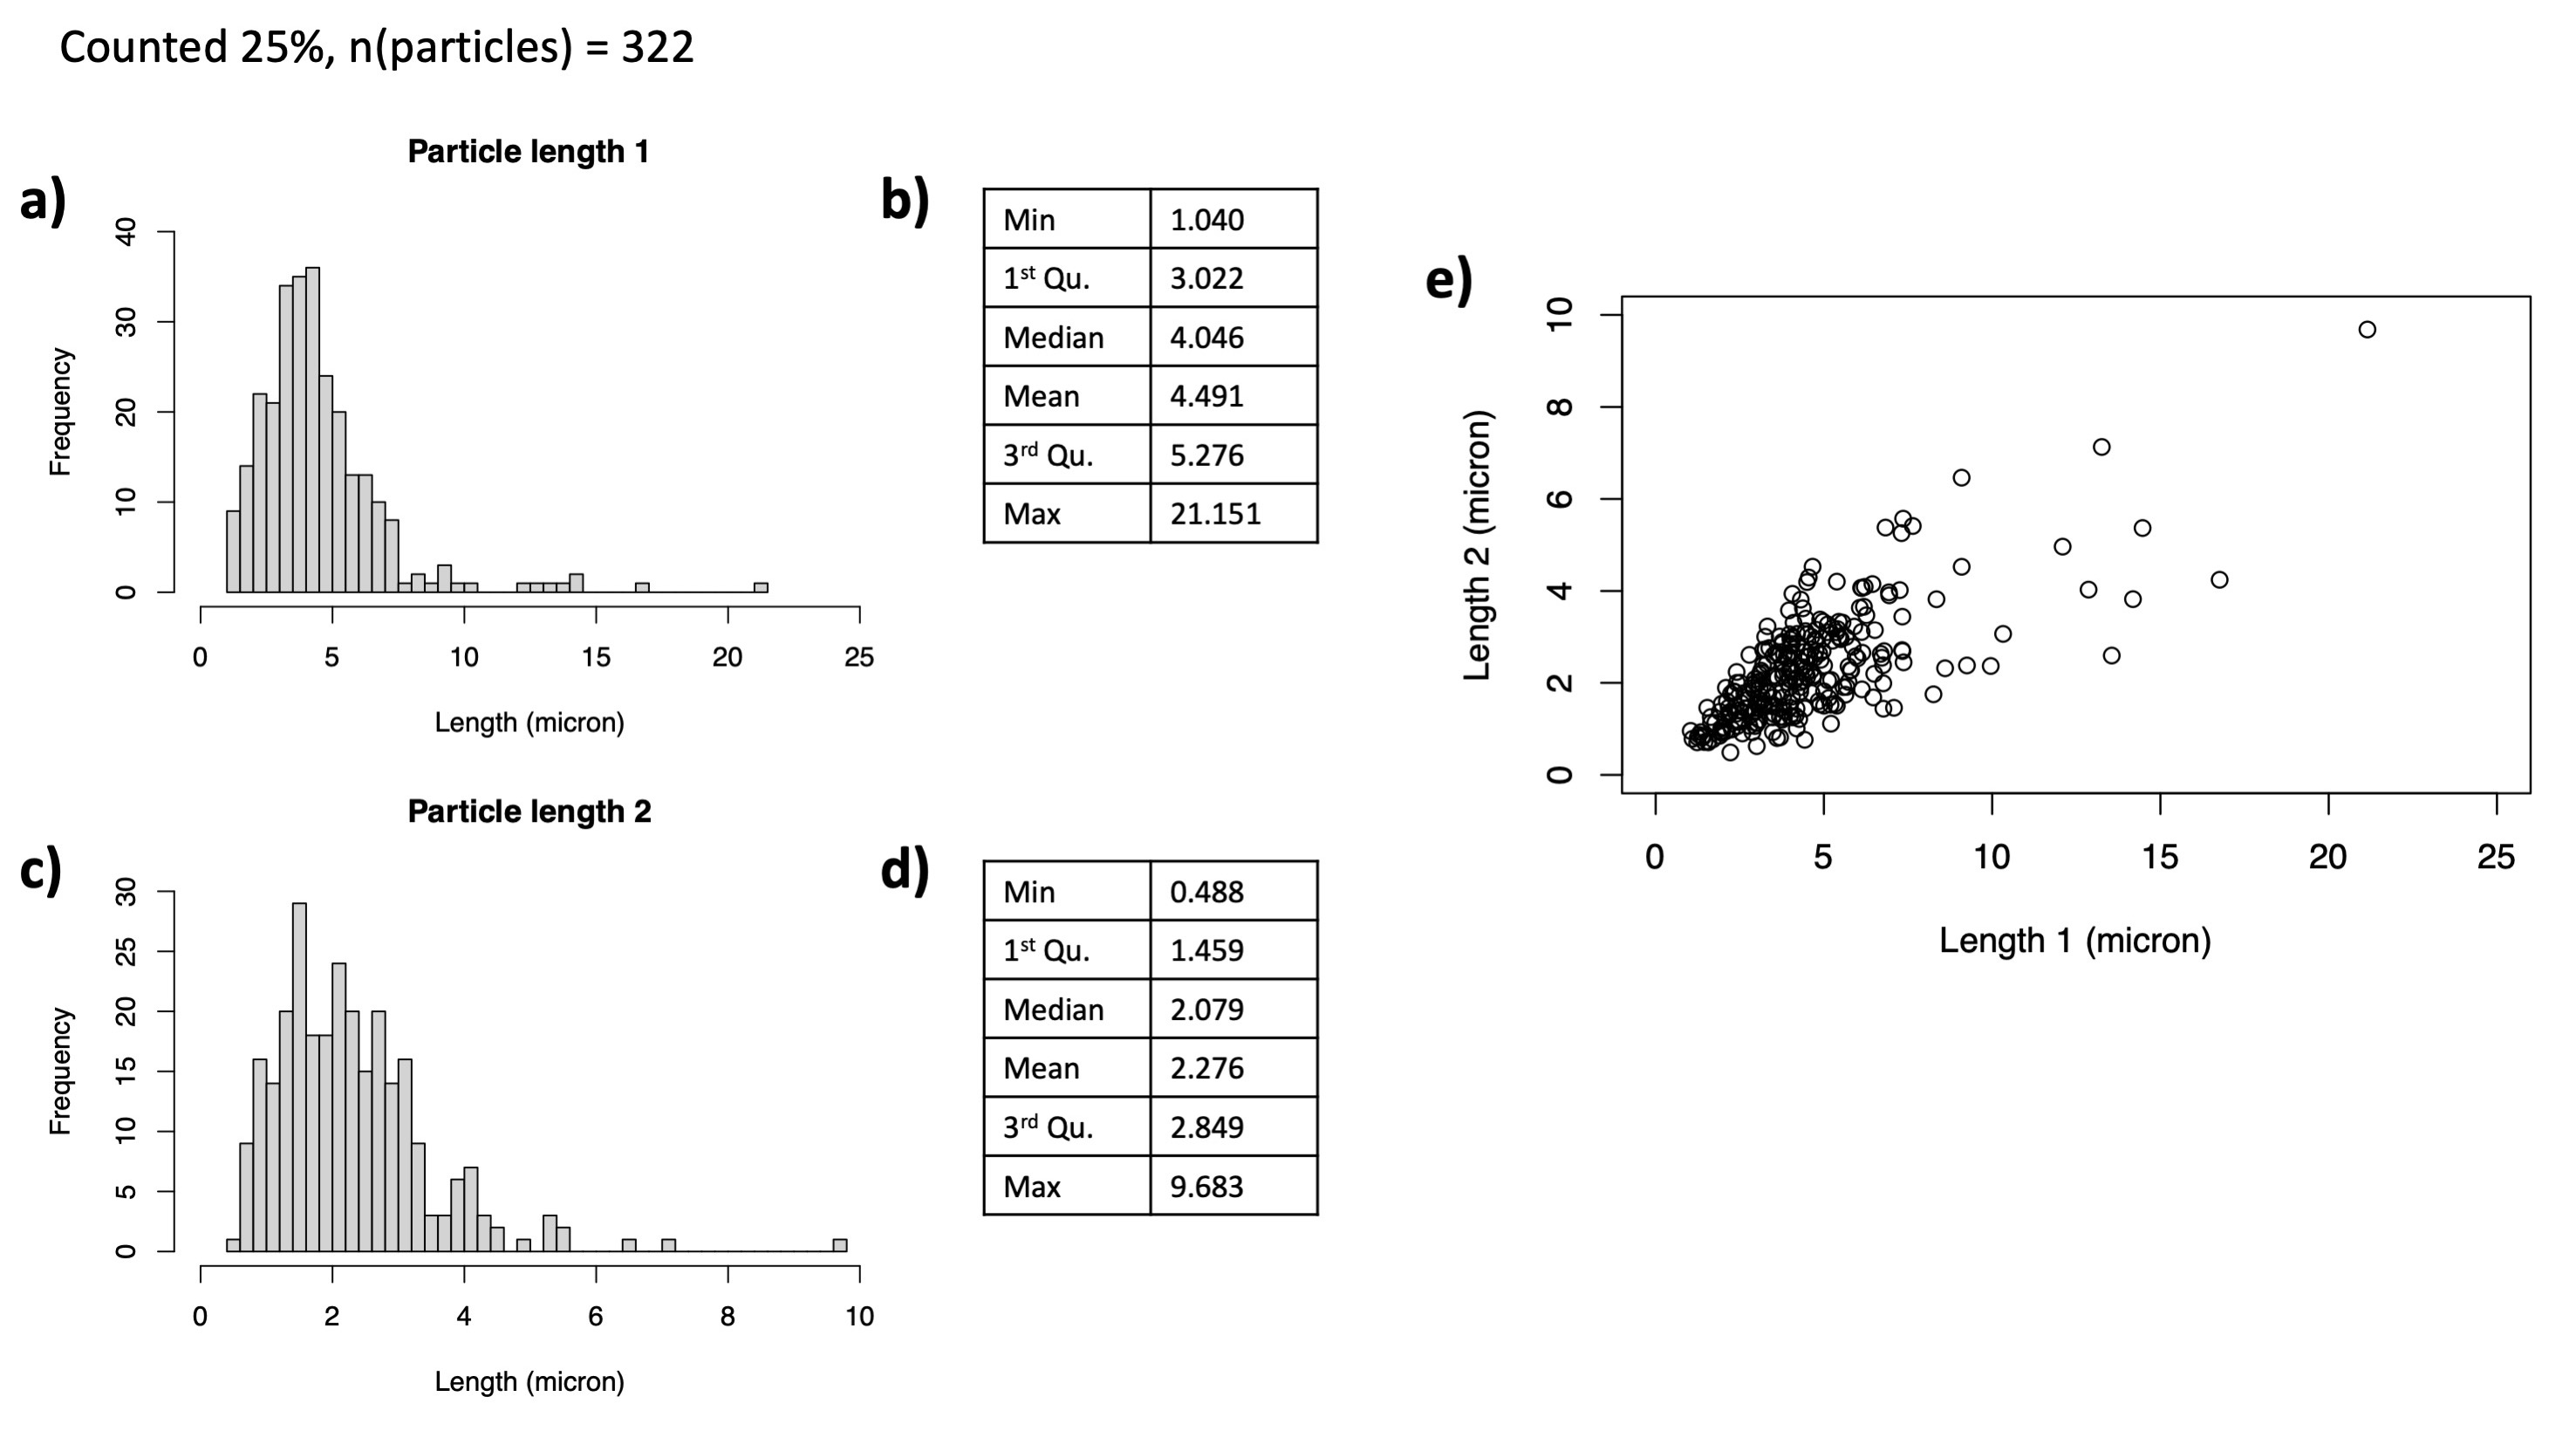
\includegraphics[width=\linewidth]{1259-19_partsize}
\caption[Particle size distribution, sample 1259.19.]{Particle size distribution of sample 1259.19: \textbf{a)} Histogram showing distribution of particle length 1 values. \textbf{b)} Descriptive statistics for particle length 1 data. \textbf{c)} Histogram showing distribution of particle length 2 values. \textbf{d)} Descriptive statistics for particle length 2 data. \textbf{e)} Graph of length 1 versus length 2 showing the degree of skew.}
\label{fig:1259.19_partsize}
\end{figure}


\section{Sample 1259.20}

SEM and dark field images of 1259.20 (\textit{Figure \ref{fig:1259.20_imgs}}) shows a thin layer of greenish blue paint with red, orange, and yellow impurities below a thick layer of modern blue overpaint. Raman confirms the pigment used in the overpaint as azurite (\textit{Figure \ref{fig:raman_1259-20}}). \textit{Figure \ref{fig:1259.20_mapdata}} presents EDS maps of both layers. Potassium, magnesium, and aluminium are present but not localised. More clearly assigned are azurite, a natural lead compounds (also containing arsenic), iron oxide, quartz, and a calcium-containing compound that may be calcite.

\textit{Figure \ref{fig:1259.20_partsize}} shows particle size data from 1259.20. Both length distributions are weighted toward the lower length values and are not very skewed.

\begin{figure}[H]
  \centering
  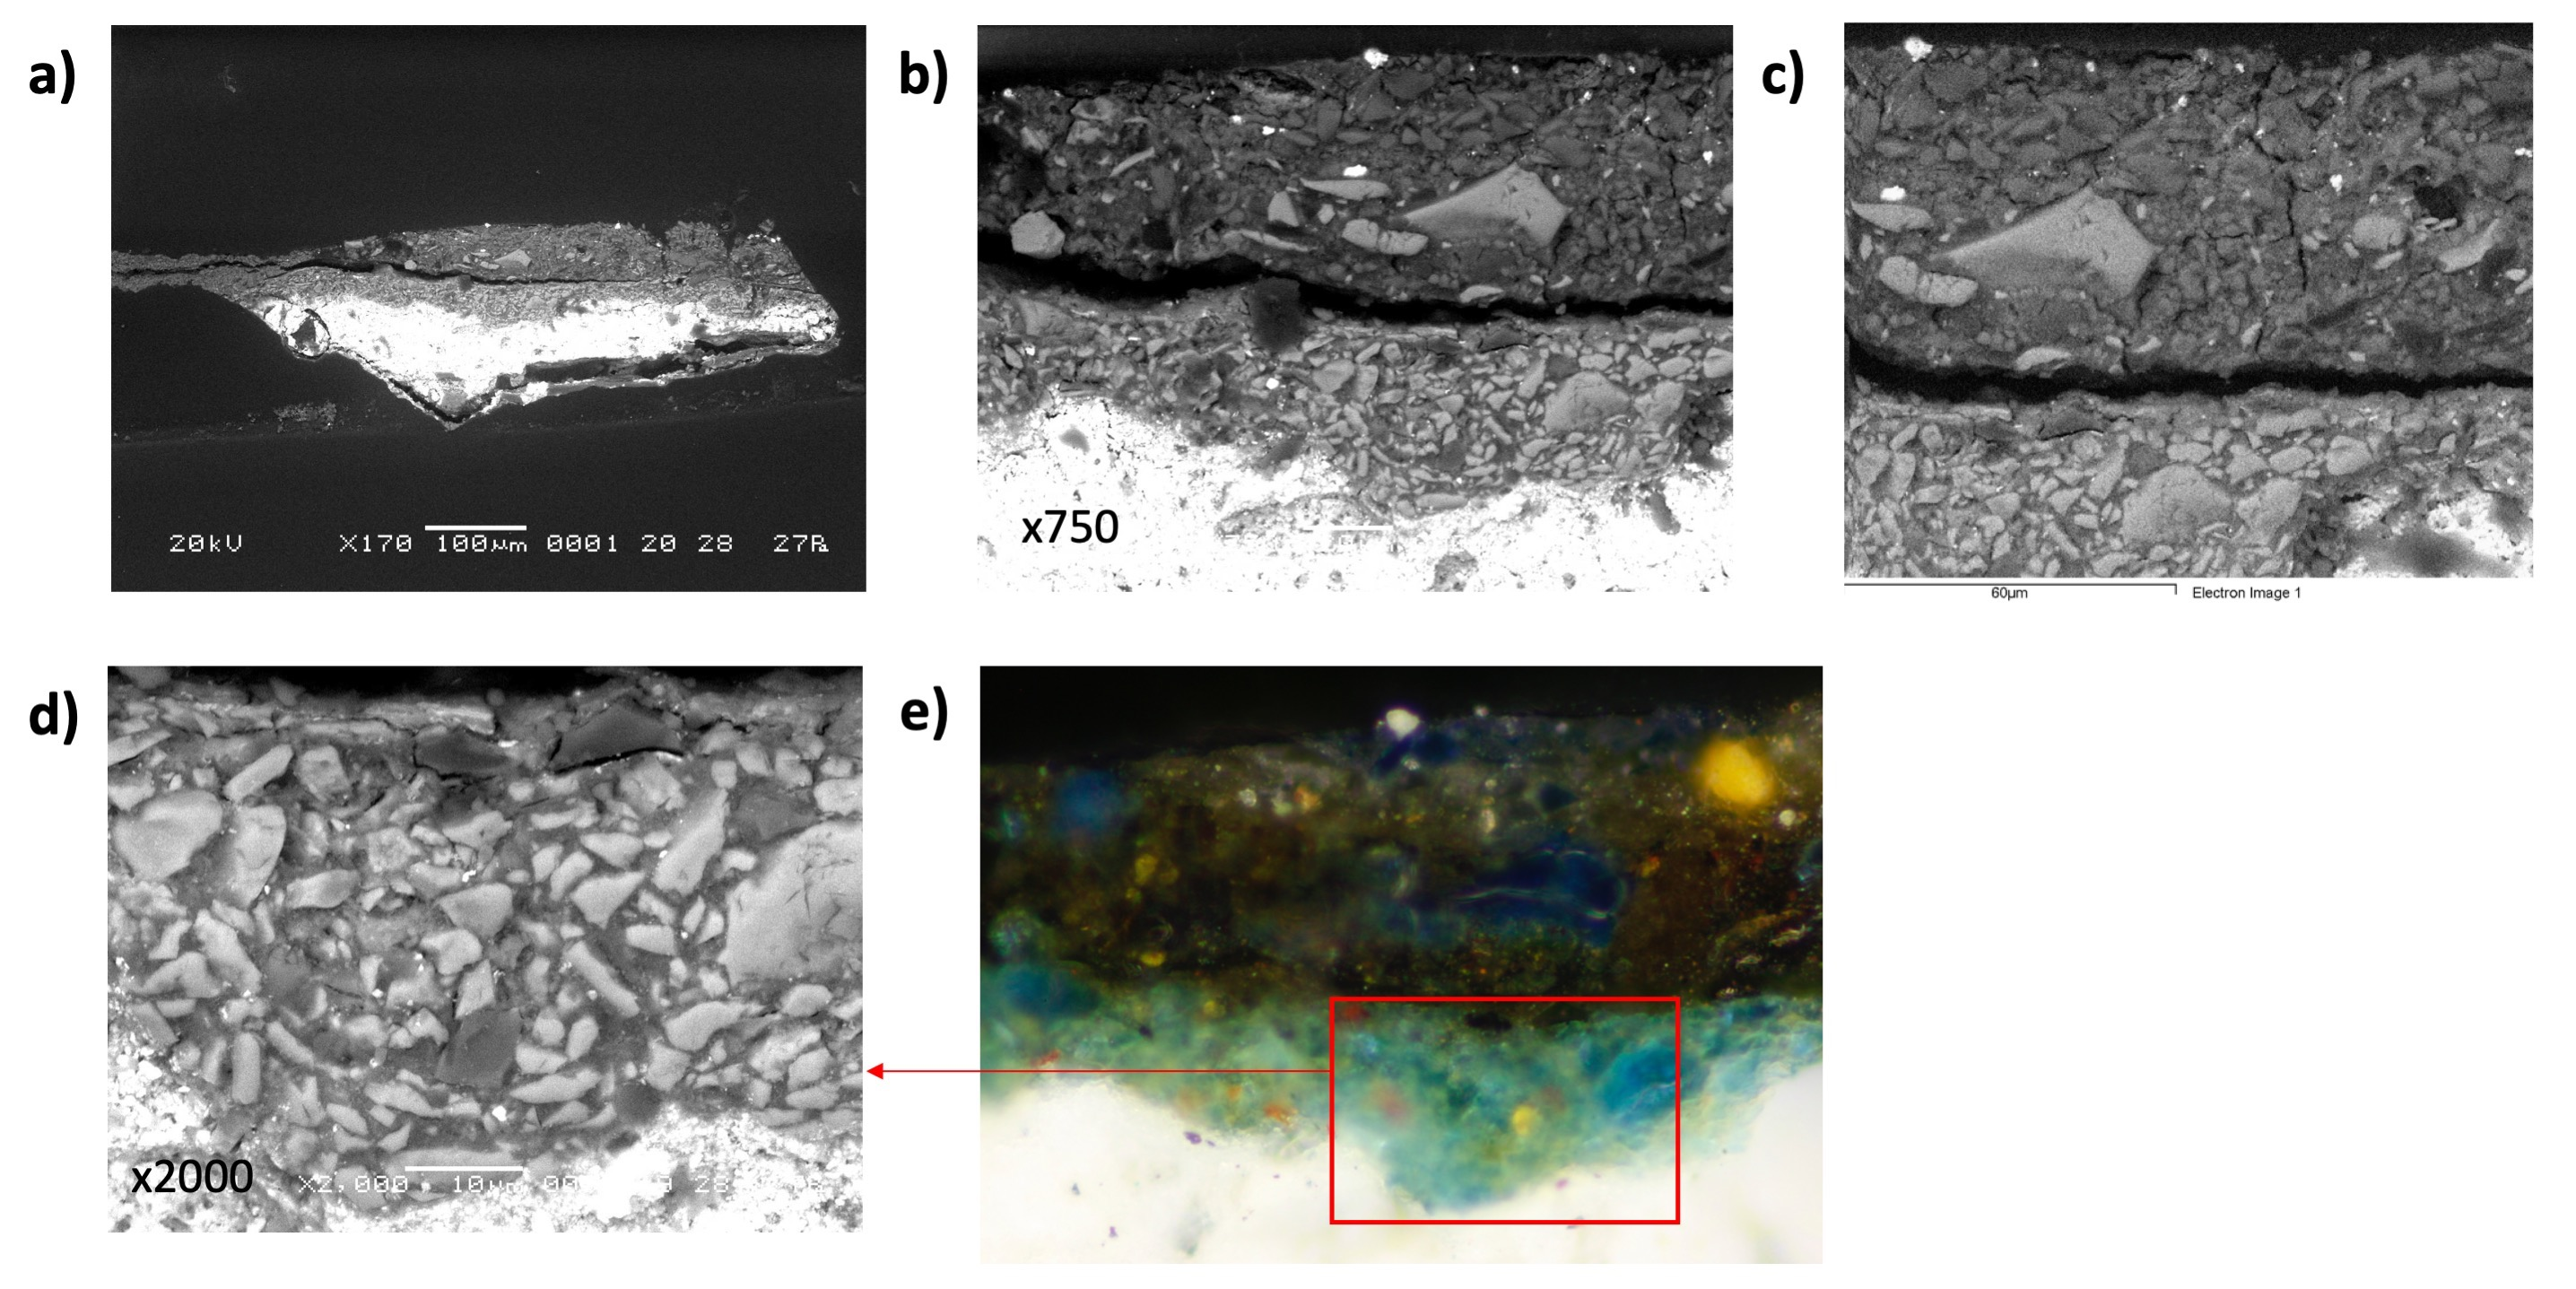
\includegraphics[width=\linewidth]{1259-20_imgs}
\caption[SEM and dark-field microscope images of sample 1259.19.]{SEM and dark-field microscope images of sample 1259.19: \textbf{a)} 170x magnification, \textbf{b)} 750x magnification, \textbf{c)} 1600x magnification, \textbf{d)} 2000x magnification, \textbf{e)} dark field microscope image provided courtesy of Katharine Waldron, HKI. The area shown in \textbf{c)} is shown in the dark field image using a red box. Darker blue overpaint layers are modern, though azurite is also used.}
\label{fig:1259.20_imgs}
\end{figure}

\begin{figure}[H] 
\centering
  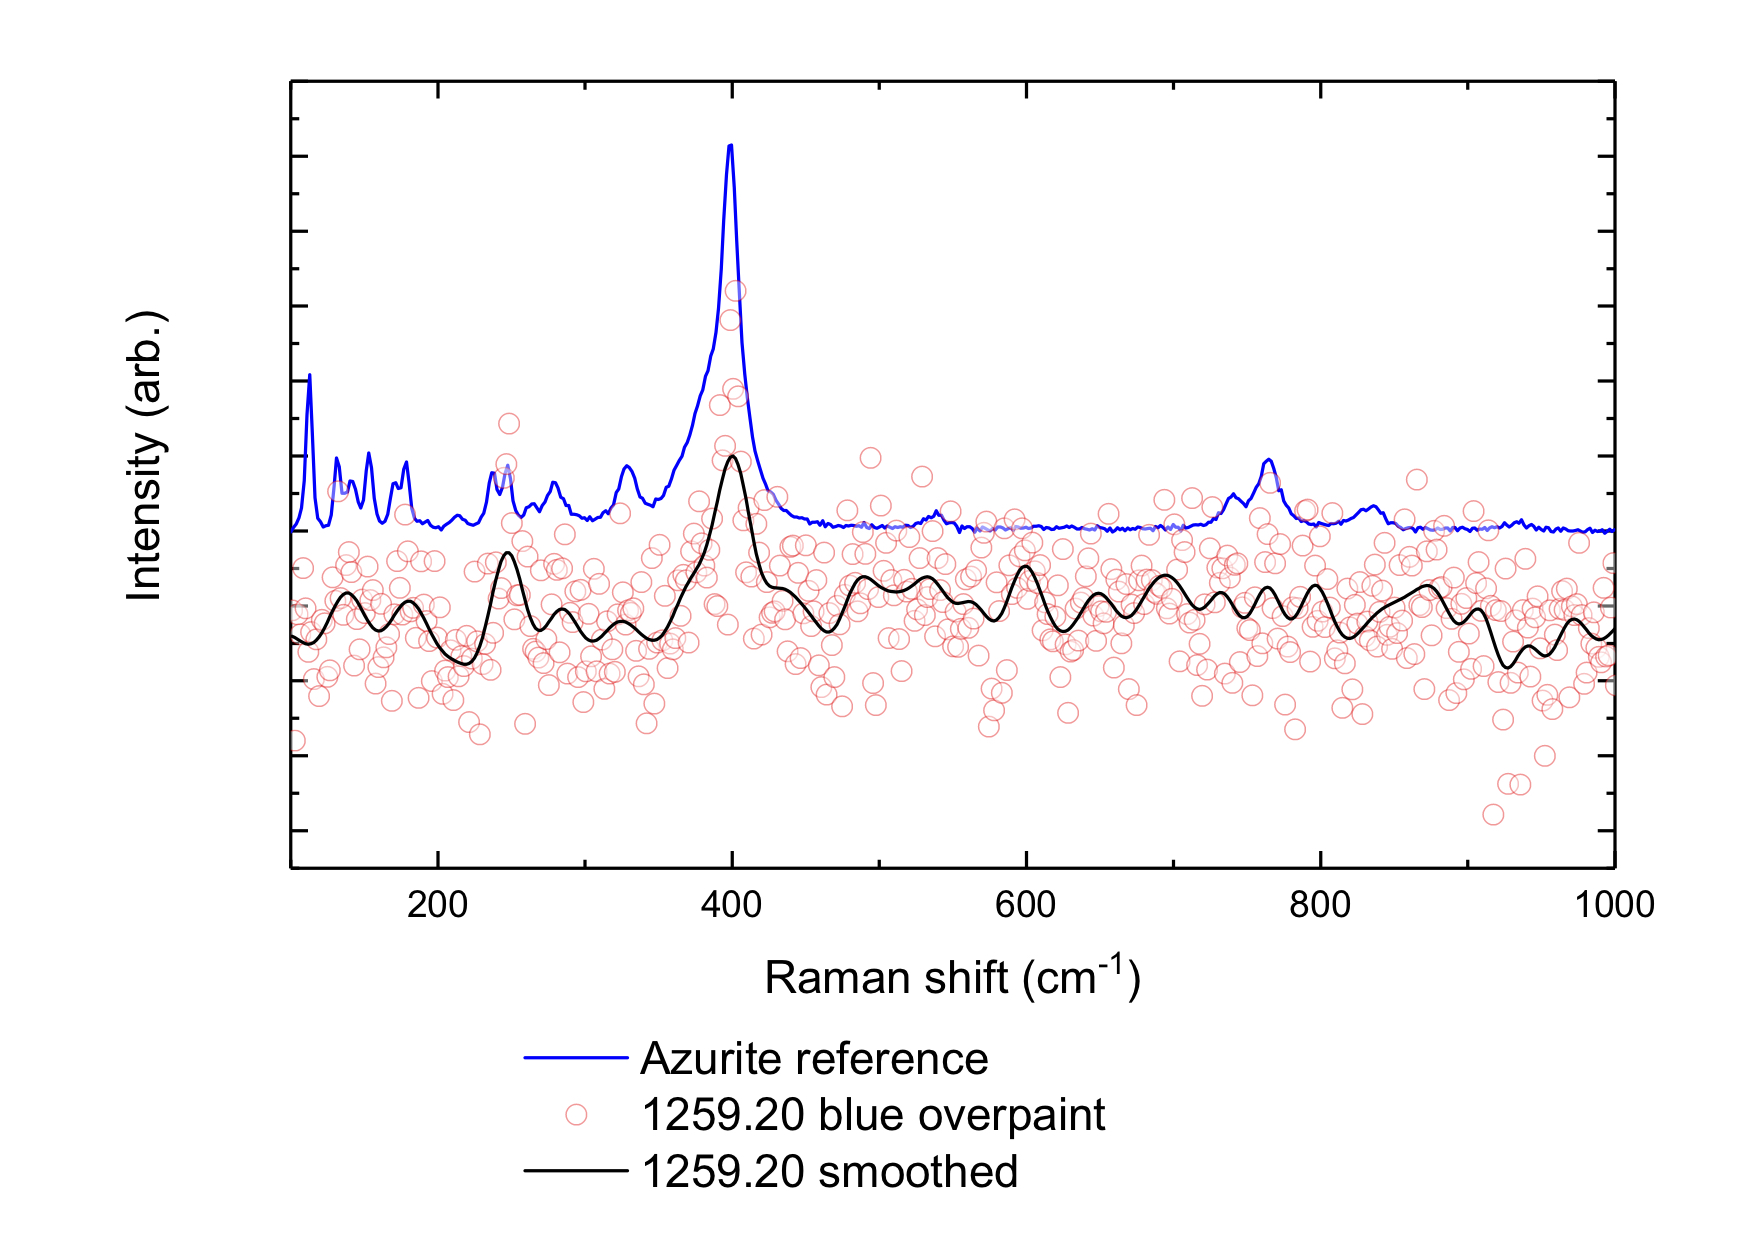
\includegraphics[width=0.8\linewidth]{1259-20_blue_overpaint}
\caption[Raman spectral data, 1259.20]{Raman spectral data: sample 1259.20. An azurite reference spectrum (blue line) is shown as a comparison to sample 1259.20 (red circles). The spectral data from 1259.20 is smoothed using an FFT filter (black line). Spectra are off-set for clarity. Although the sample spectra suffer from low intensities compared to fluorescence from the surrounding resin, the characteristic band at 400 cm\textsuperscript{-1} is visible, confirming the presence of azurite.}
\label{fig:raman_1259-20}
\end{figure}

\begin{figure}[H]
\centering
\begin{minipage}[t]{\linewidth}
  \centering
  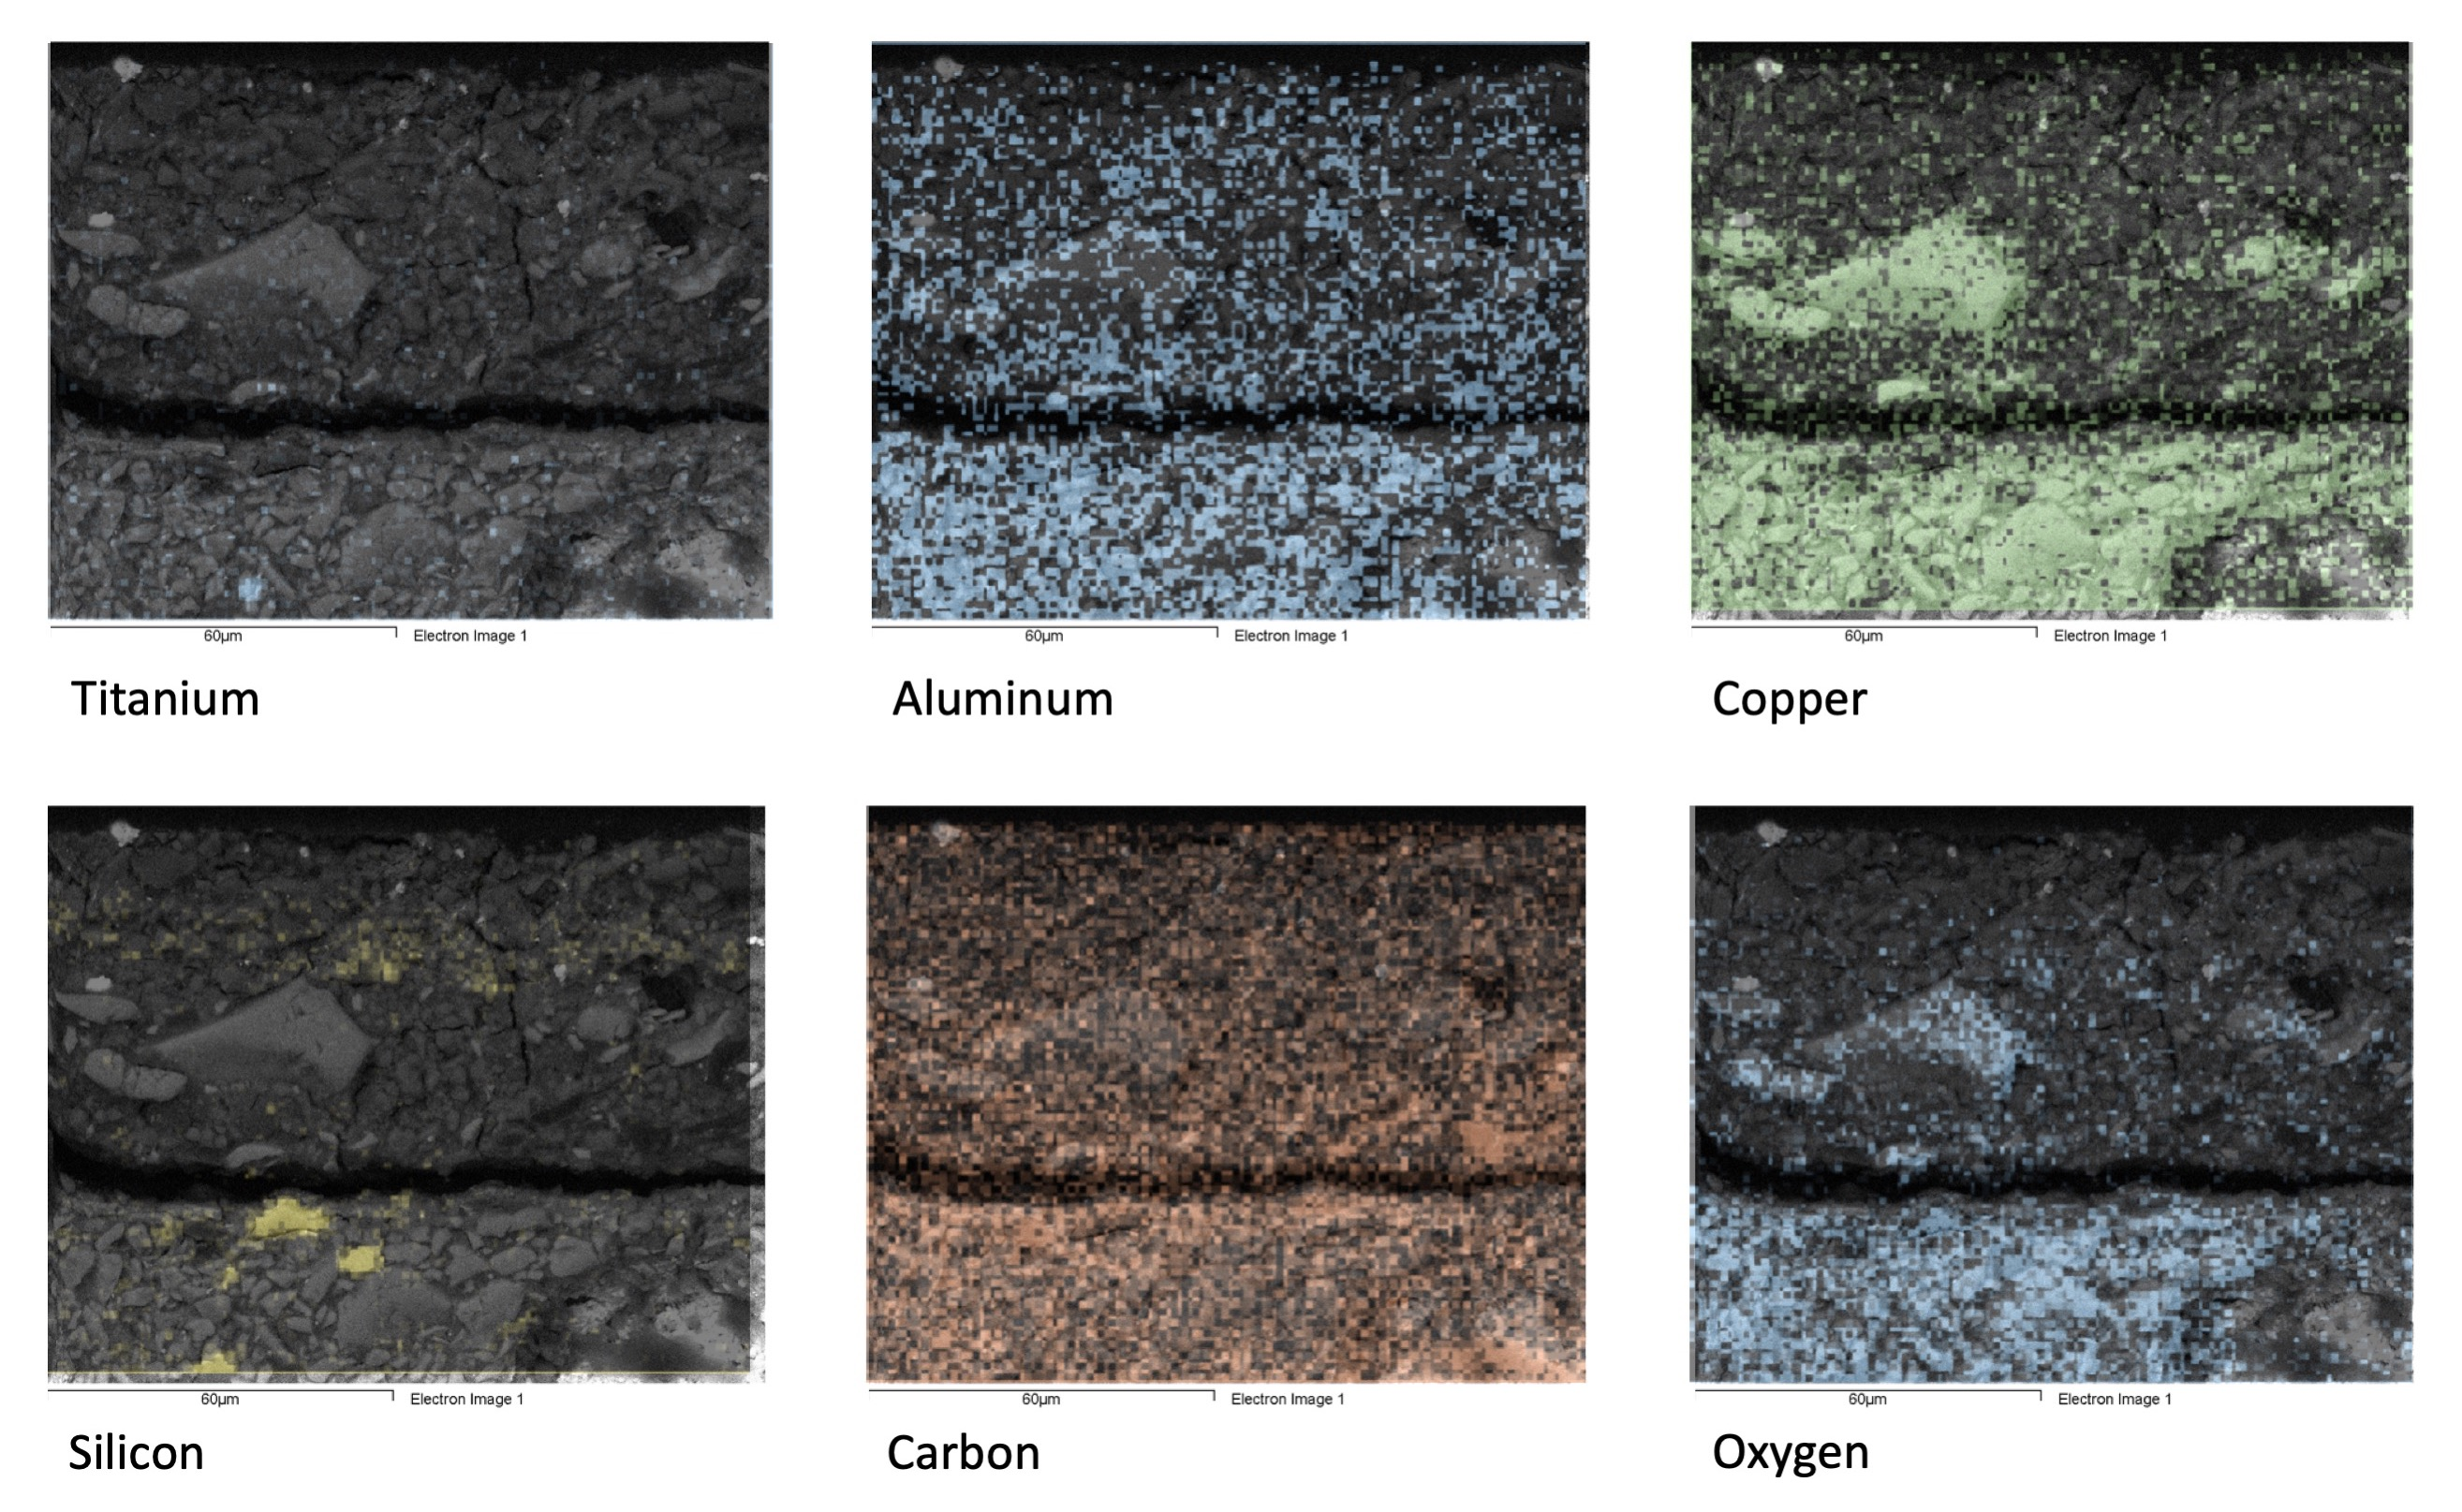
\includegraphics[width=0.9\linewidth]{1259-20_mapdata_1}
\hfill
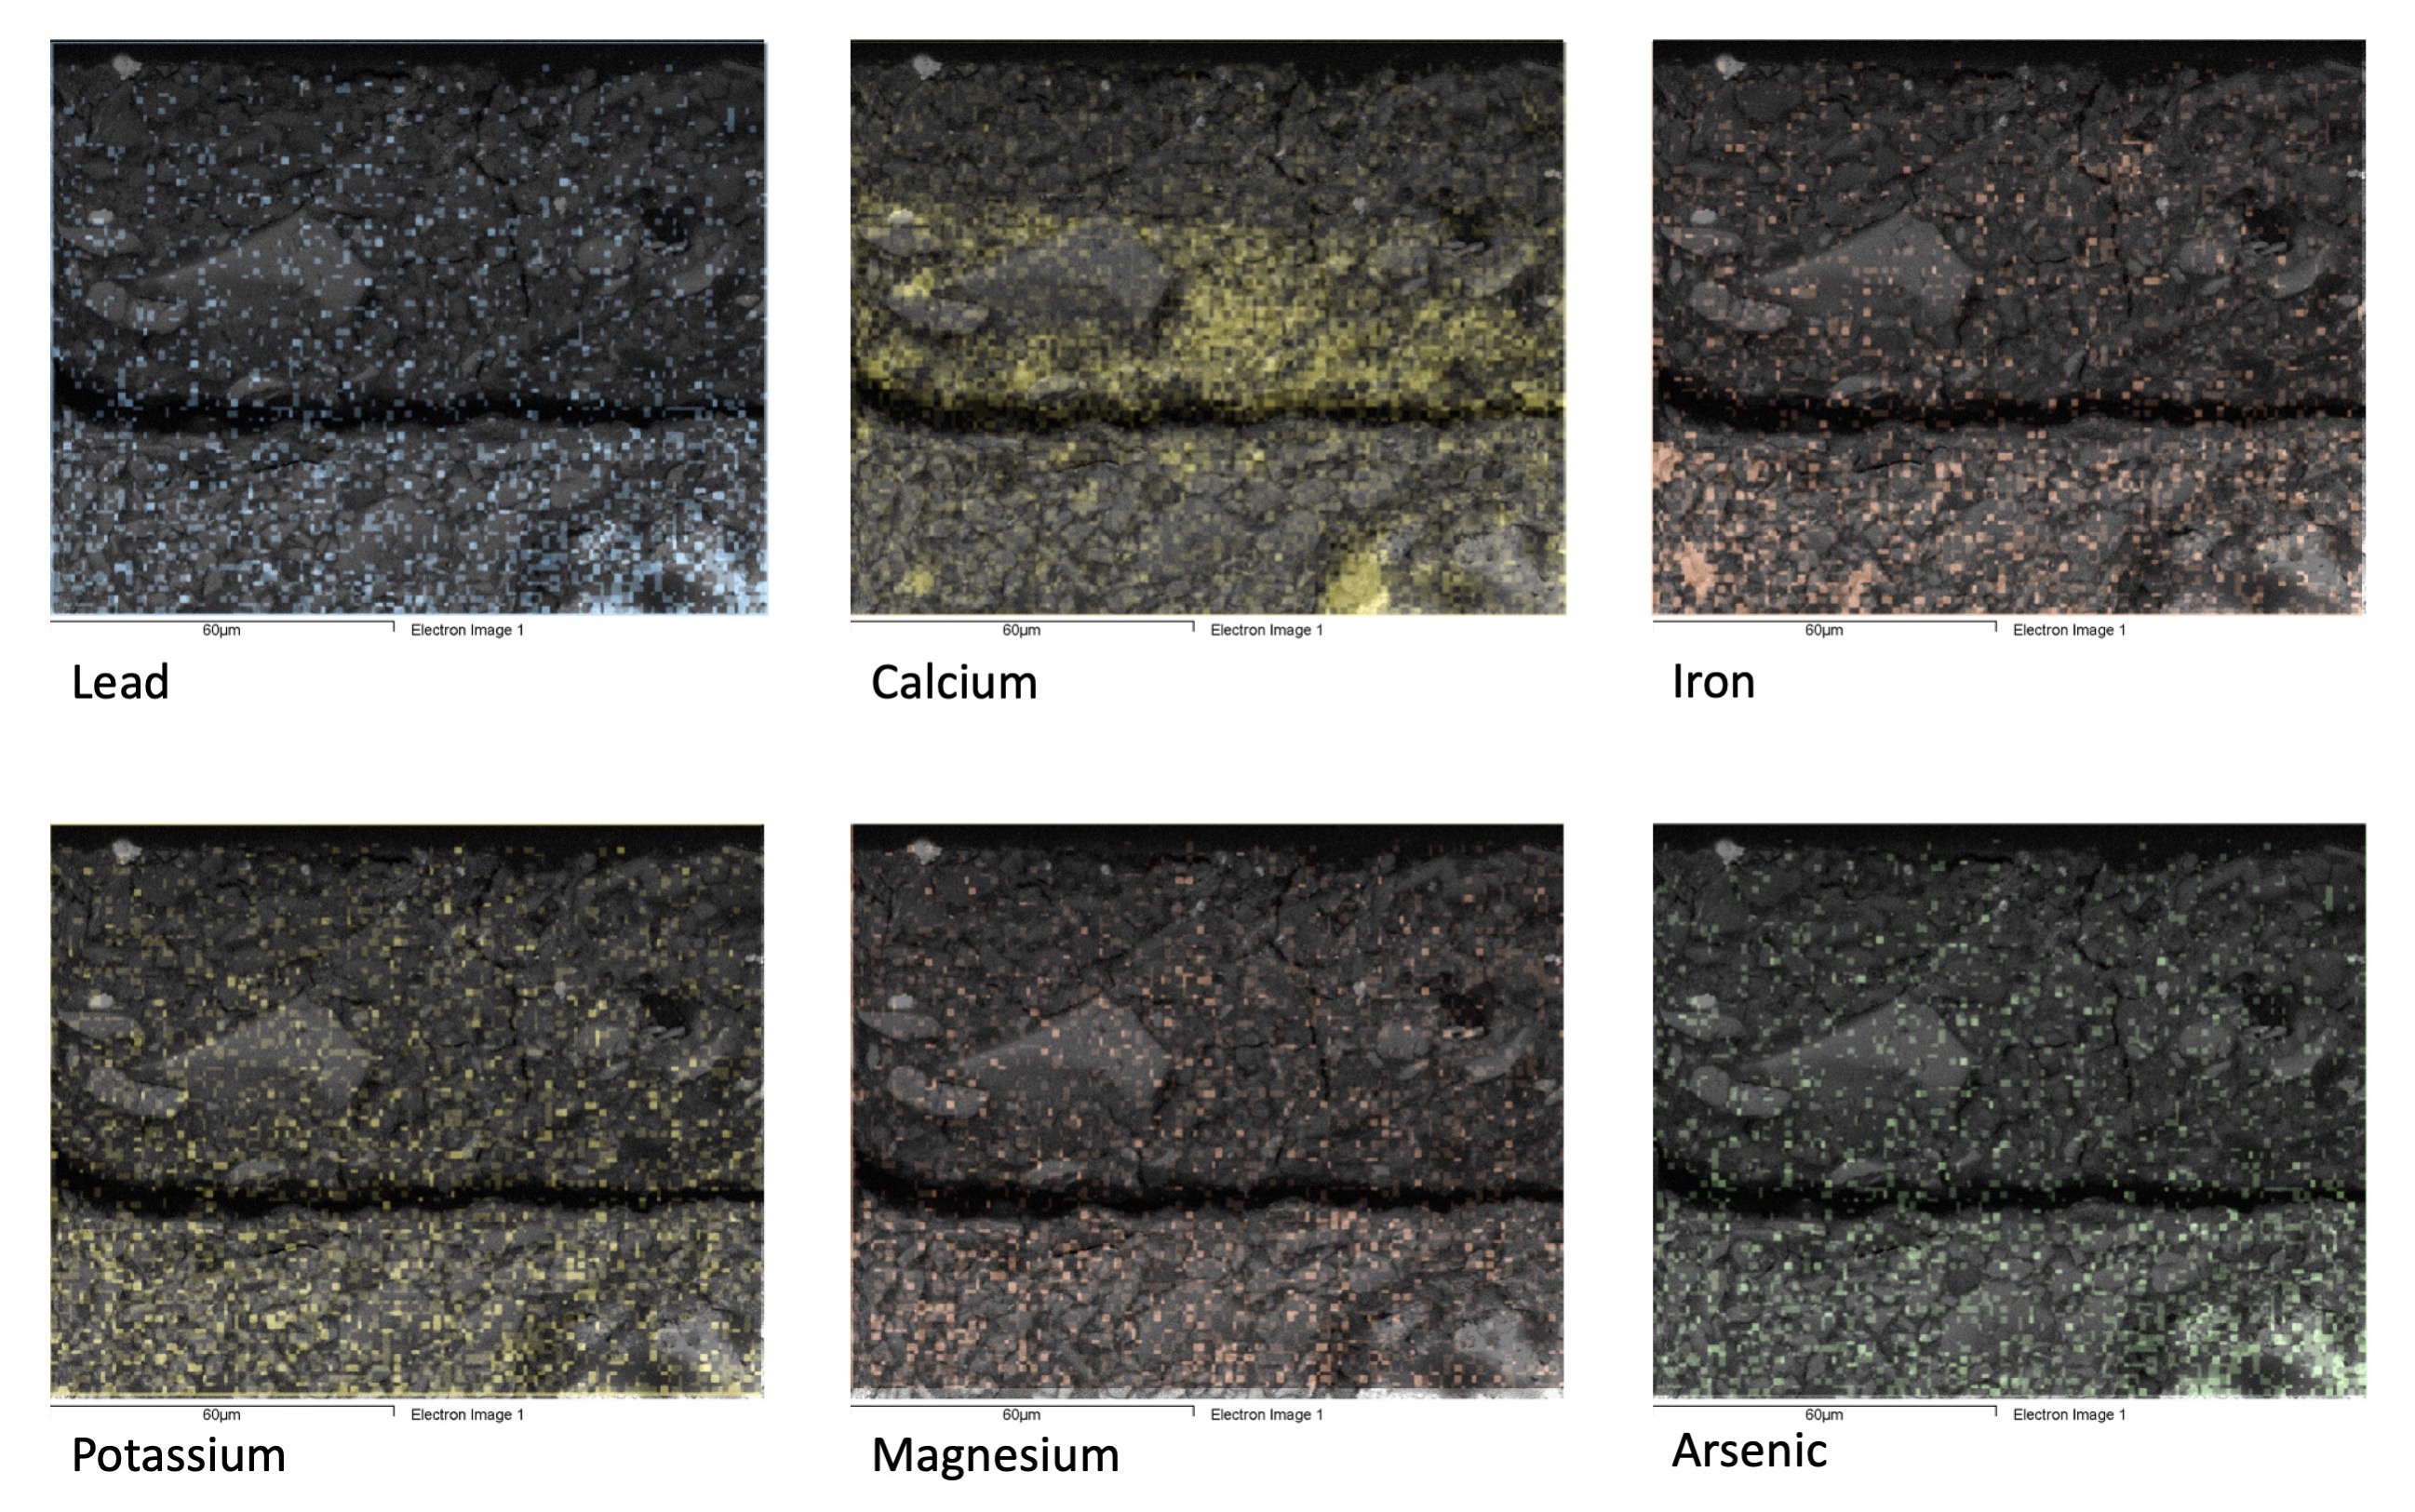
\includegraphics[width=0.9\linewidth]{1259-20_mapdata_2}
\hfill
\end{minipage}
\caption[EDS map data, sample 1259.20.]{EDS map data of sample 1259.20 showing locations of elements in an area of the azurite paint layer. Elements detected are Ti, Al, Cu, Si, C, O, Pb, Ca, Fe, K, Mg, and As.}
\label{fig:1259.20_mapdata}
\end{figure}

\begin{figure}[H]
\centering
  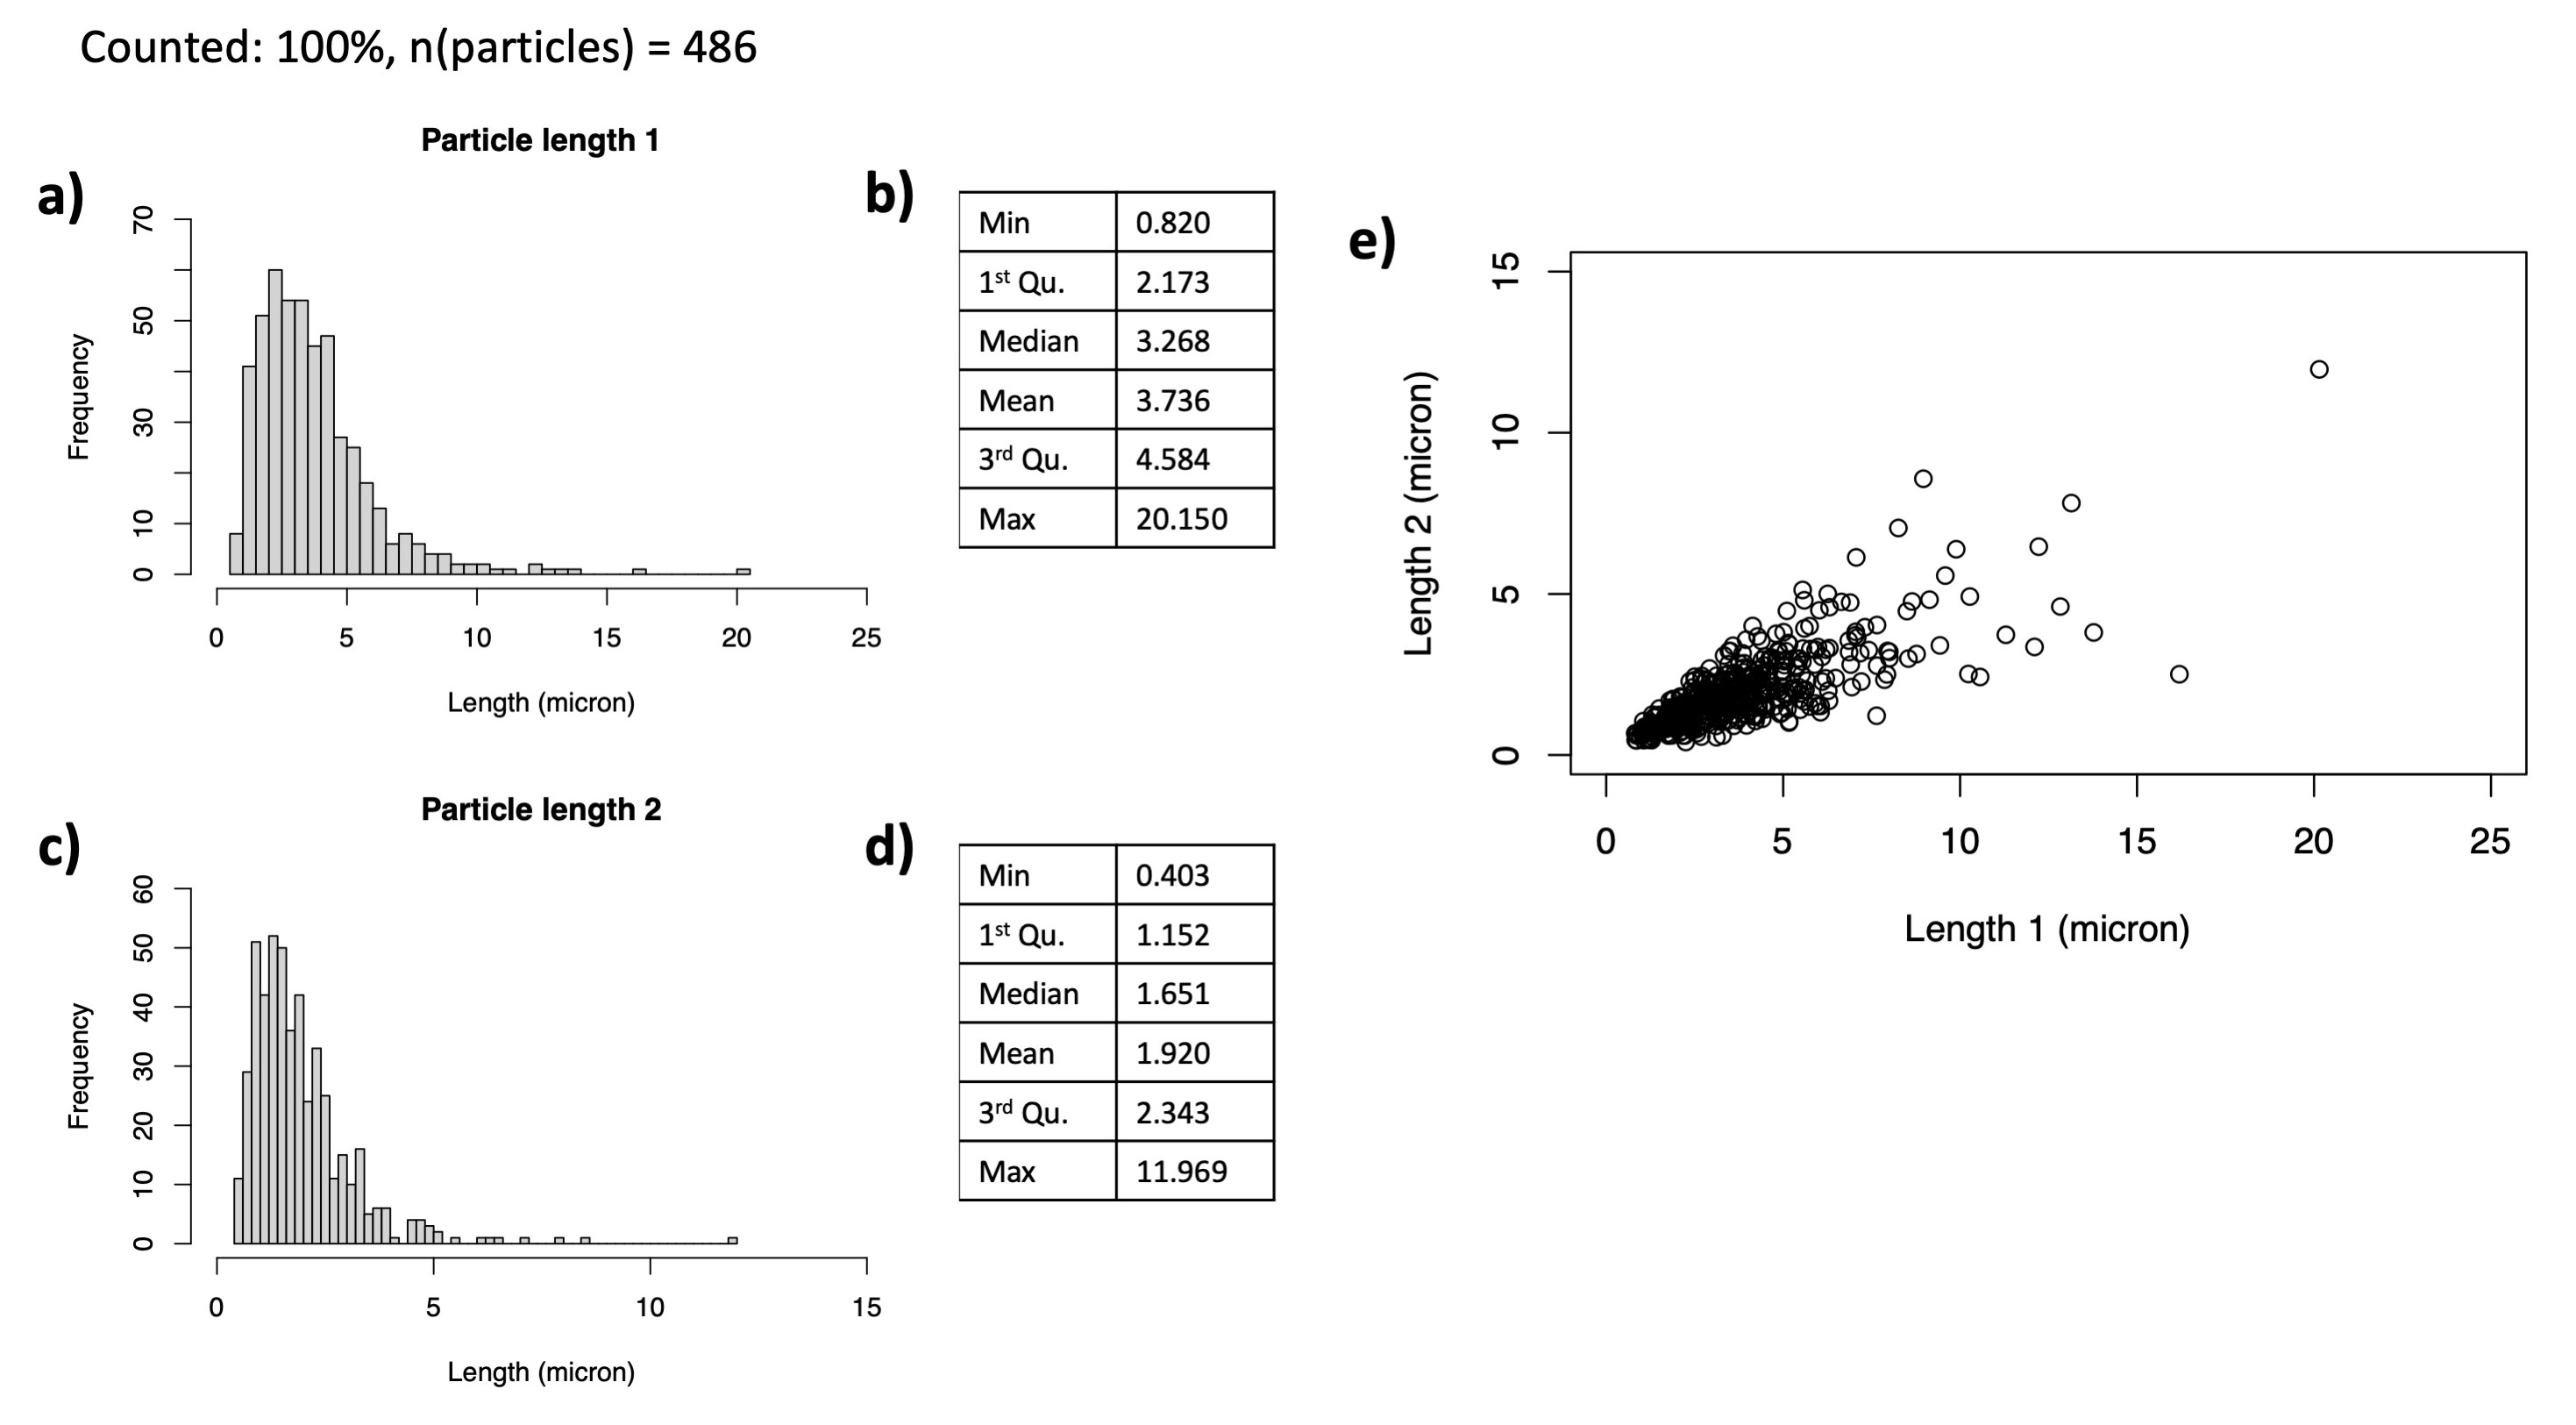
\includegraphics[width=\linewidth]{1259-20_partsize}
\caption[Particle size distribution, sample 1259.20.]{Particle size distribution of sample 1259.20: \textbf{a)} Histogram showing distribution of particle length 1 values. \textbf{b)} Descriptive statistics for particle length 1 data. \textbf{c)} Histogram showing distribution of particle length 2 values. \textbf{d)} Descriptive statistics for particle length 2 data. \textbf{e)} Graph of length 1 versus length 2 showing the degree of skew.}
\label{fig:1259.20_partsize}
\end{figure}



\section{Sample 1259.21}

SEM images of 1259.21 (\textit{Figure \ref{fig:1259.21_imgs}}) show three distinct layers, the bottom one comprised of smaller azurite pigments as well as lead white and vermilion, and the upper two comprised of larger smalt particles. 

EDS point spectra (\textit{Figure \ref{fig:1259.21_pointspec}}) confirm that the red particles in the azurite layer are mercury sulfide, vermilion. EDS map data, shown in \textit{Figure \ref{fig:1259.21_mapdata}}, confirms azurite as the blue pigment of the lower paint layer as well as smalt in the upper right of the map image in the upper blue layer (marked by the presence of silicon and potassium). Quartz, rutile, lead white, vermillion (mercury), calcite, and dolomite are also indicated. Cobalt, a component of smalt, does not show clear localisation, possibly due to low abundance. Iron is also not localised in the map.

Particle size data, in \textit{Figure \ref{fig:1259.21_partsize}}, shows average length values of 4.94 and 2.63 $\mu$m, with several very large outliers. Particles are biased toward longer, thinner shapes.

\begin{figure}[H]
  \centering
  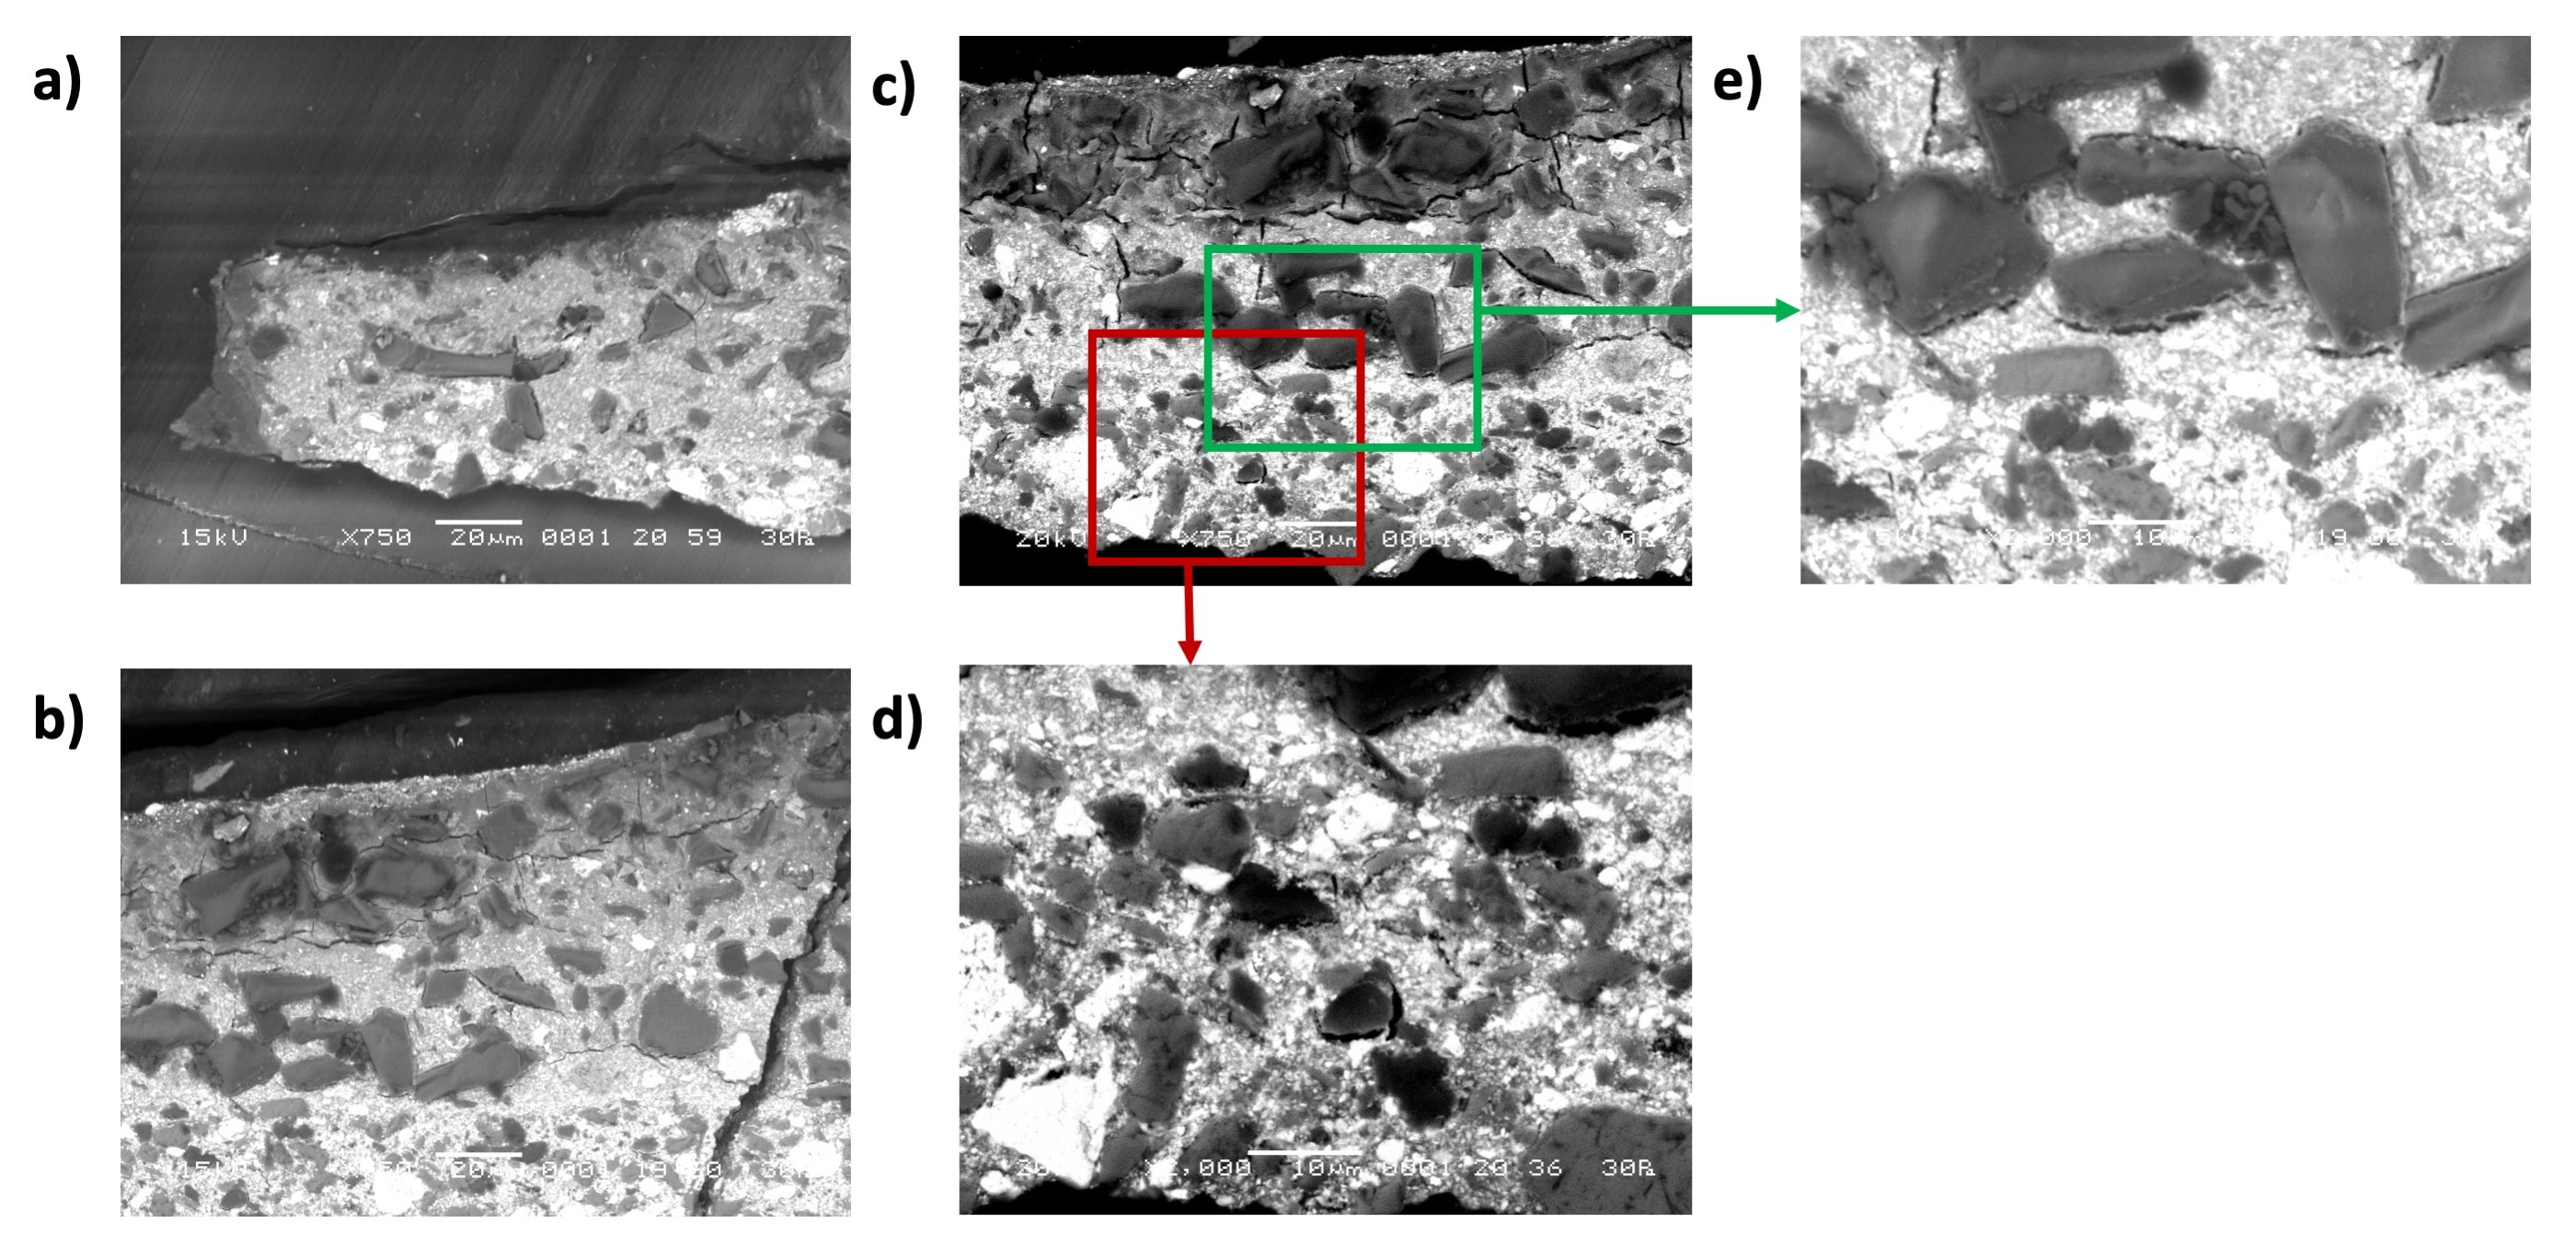
\includegraphics[width=\linewidth]{1259-21_imgs}
\caption[SEM images of sample 1259.21.]{SEM images of sample 1259.21: \textbf{a)} 750x magnification, \textbf{b)} 750x magnification, \textbf{c)} 750x magnification, \textbf{d)} 2000x magnification, \textbf{e)} 2000x magnification. Red and green boxes show the areas of \textbf{c} corresponding to images \textbf{d} and \textbf{e}.}
\label{fig:1259.21_imgs}
\end{figure}

\begin{figure}[H]
  \centering
  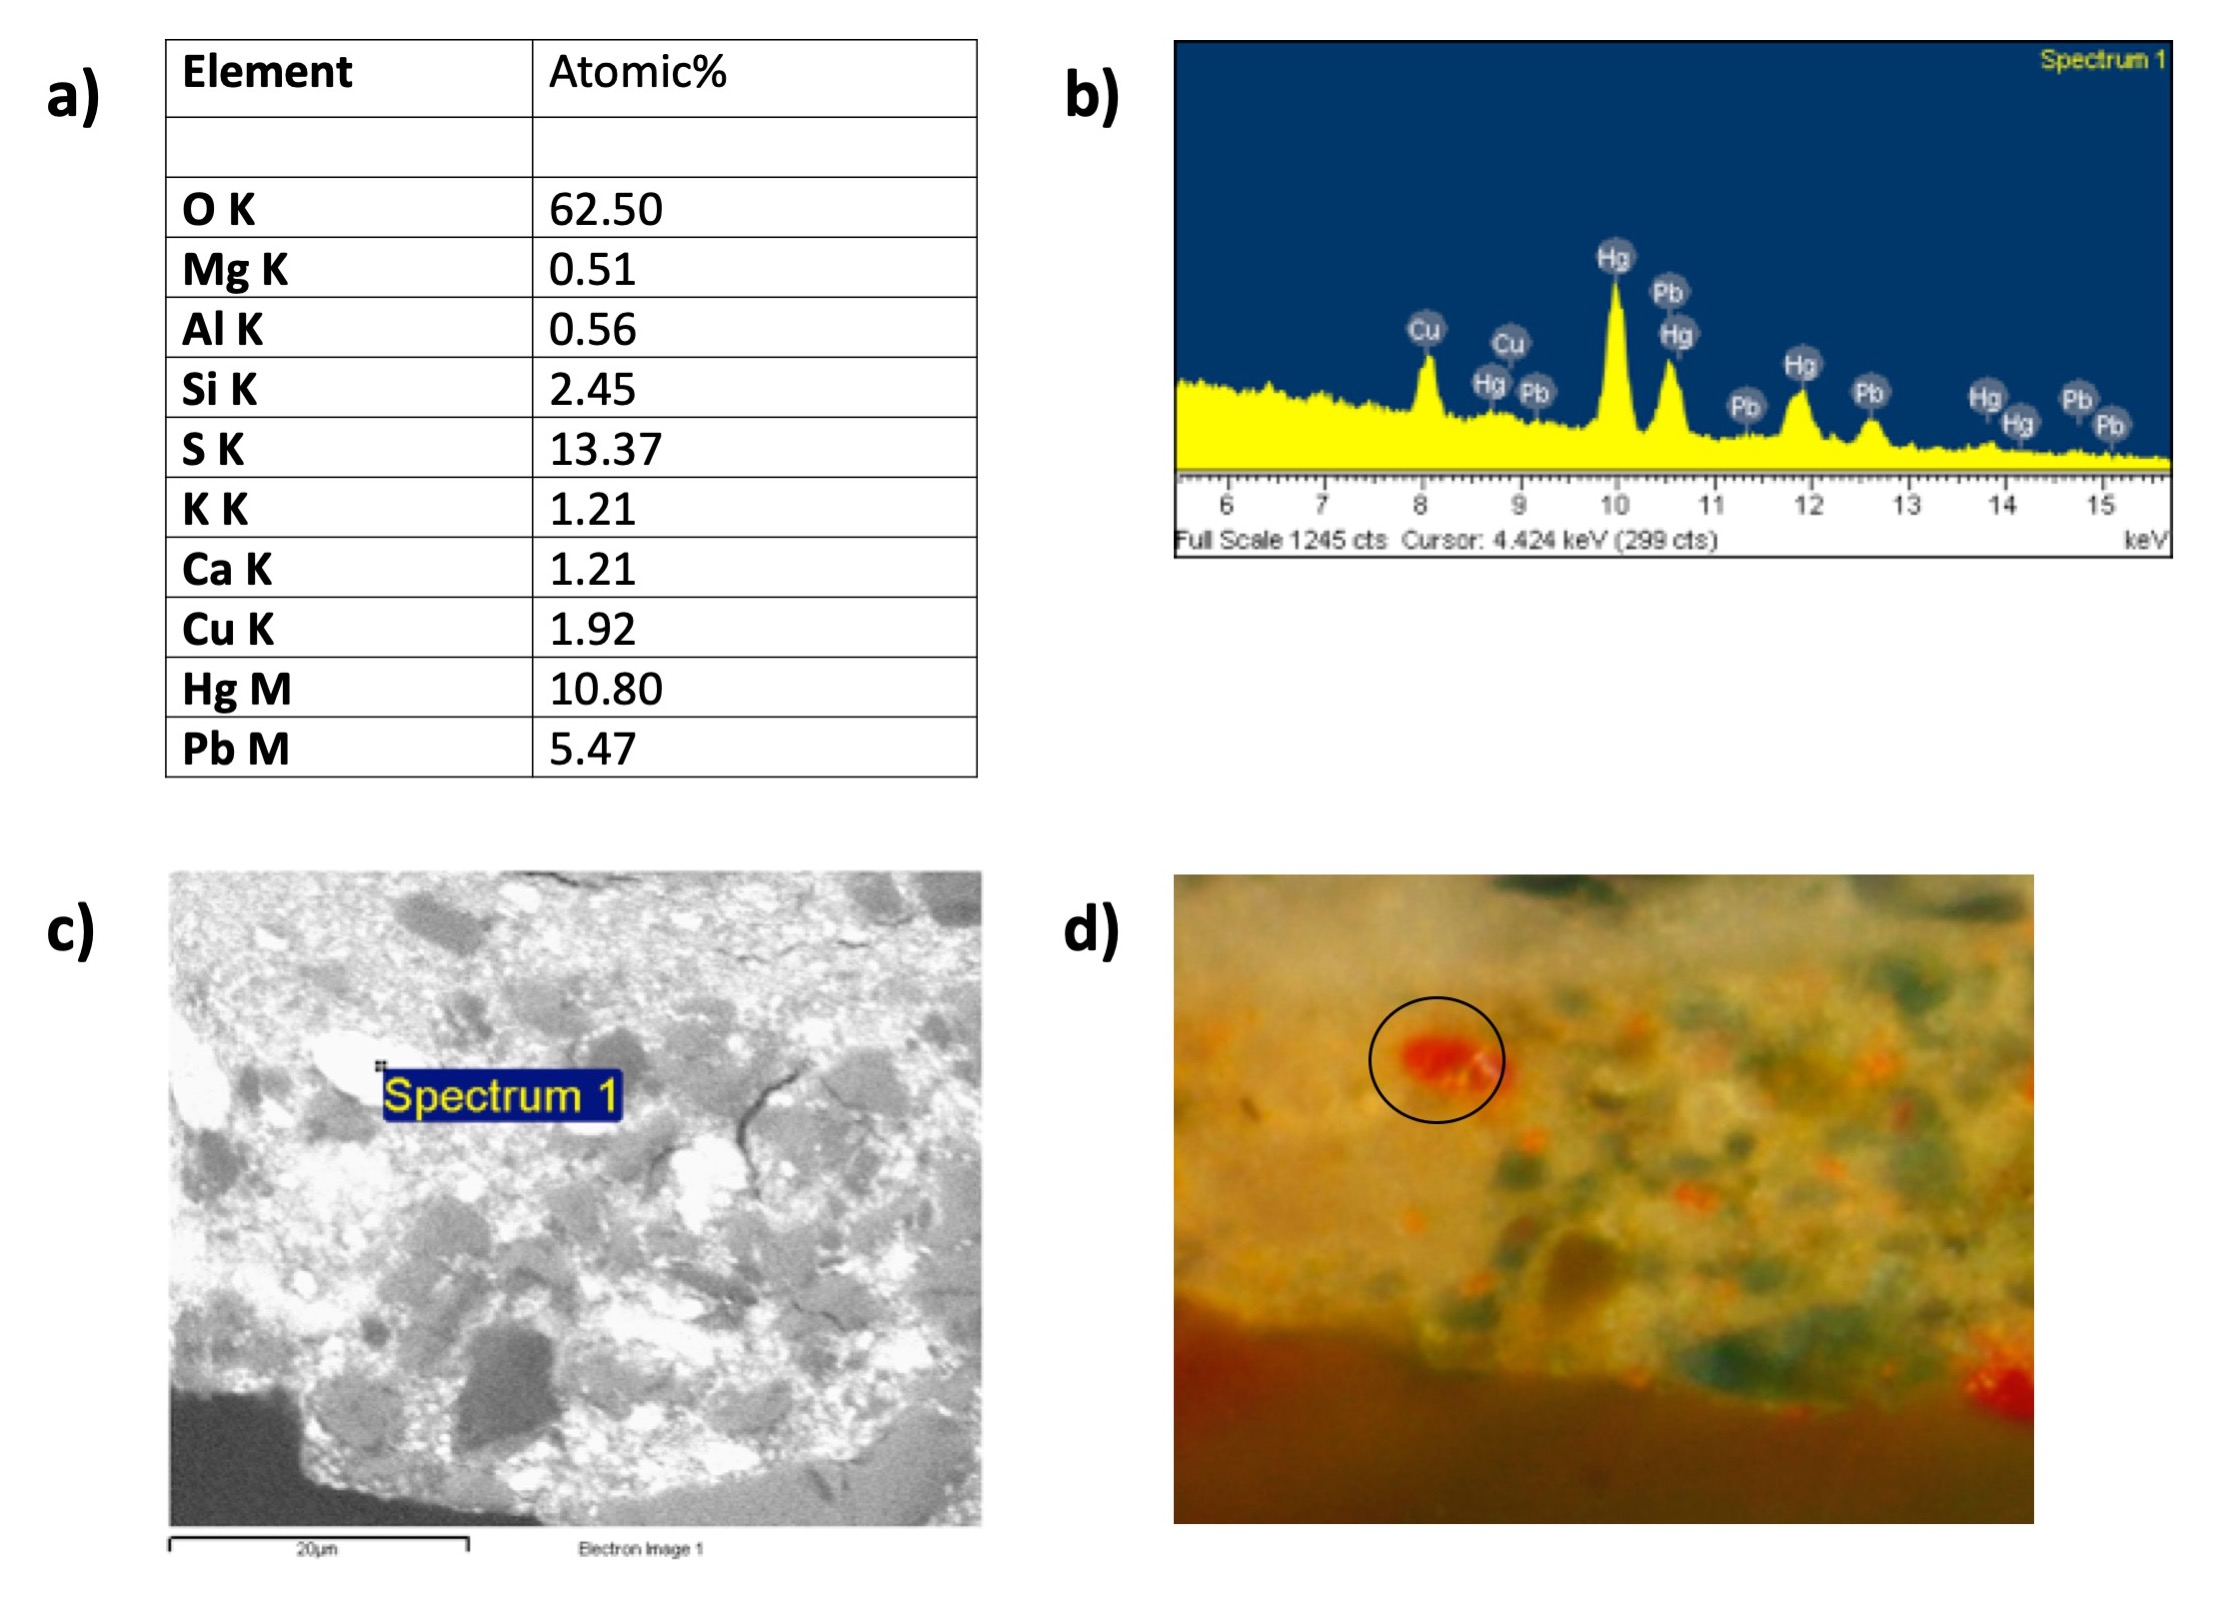
\includegraphics[width=\linewidth]{1259-21_pointspec}
\caption[EDS point spectrum data, sample 1259.21.]{EDS point spectrum data, sample 1259.21: \textbf{a)} Quantitative EDS results of red pigment particle showing high levels of mercury and sulfur, \textbf{b)} Detail area of EDS spectrum showing detection of mercury and sulfur, \textbf{c)} SEM image showing point spectrum location, \textbf{d)} dark field microscope image showing point spectrum sample location. Image is provided courtesy of Katharine Waldron, HKI.}
\label{fig:1259.21_pointspec}
\end{figure}

\begin{figure}[H]
\centering
\begin{minipage}[t]{\linewidth}
  \centering
  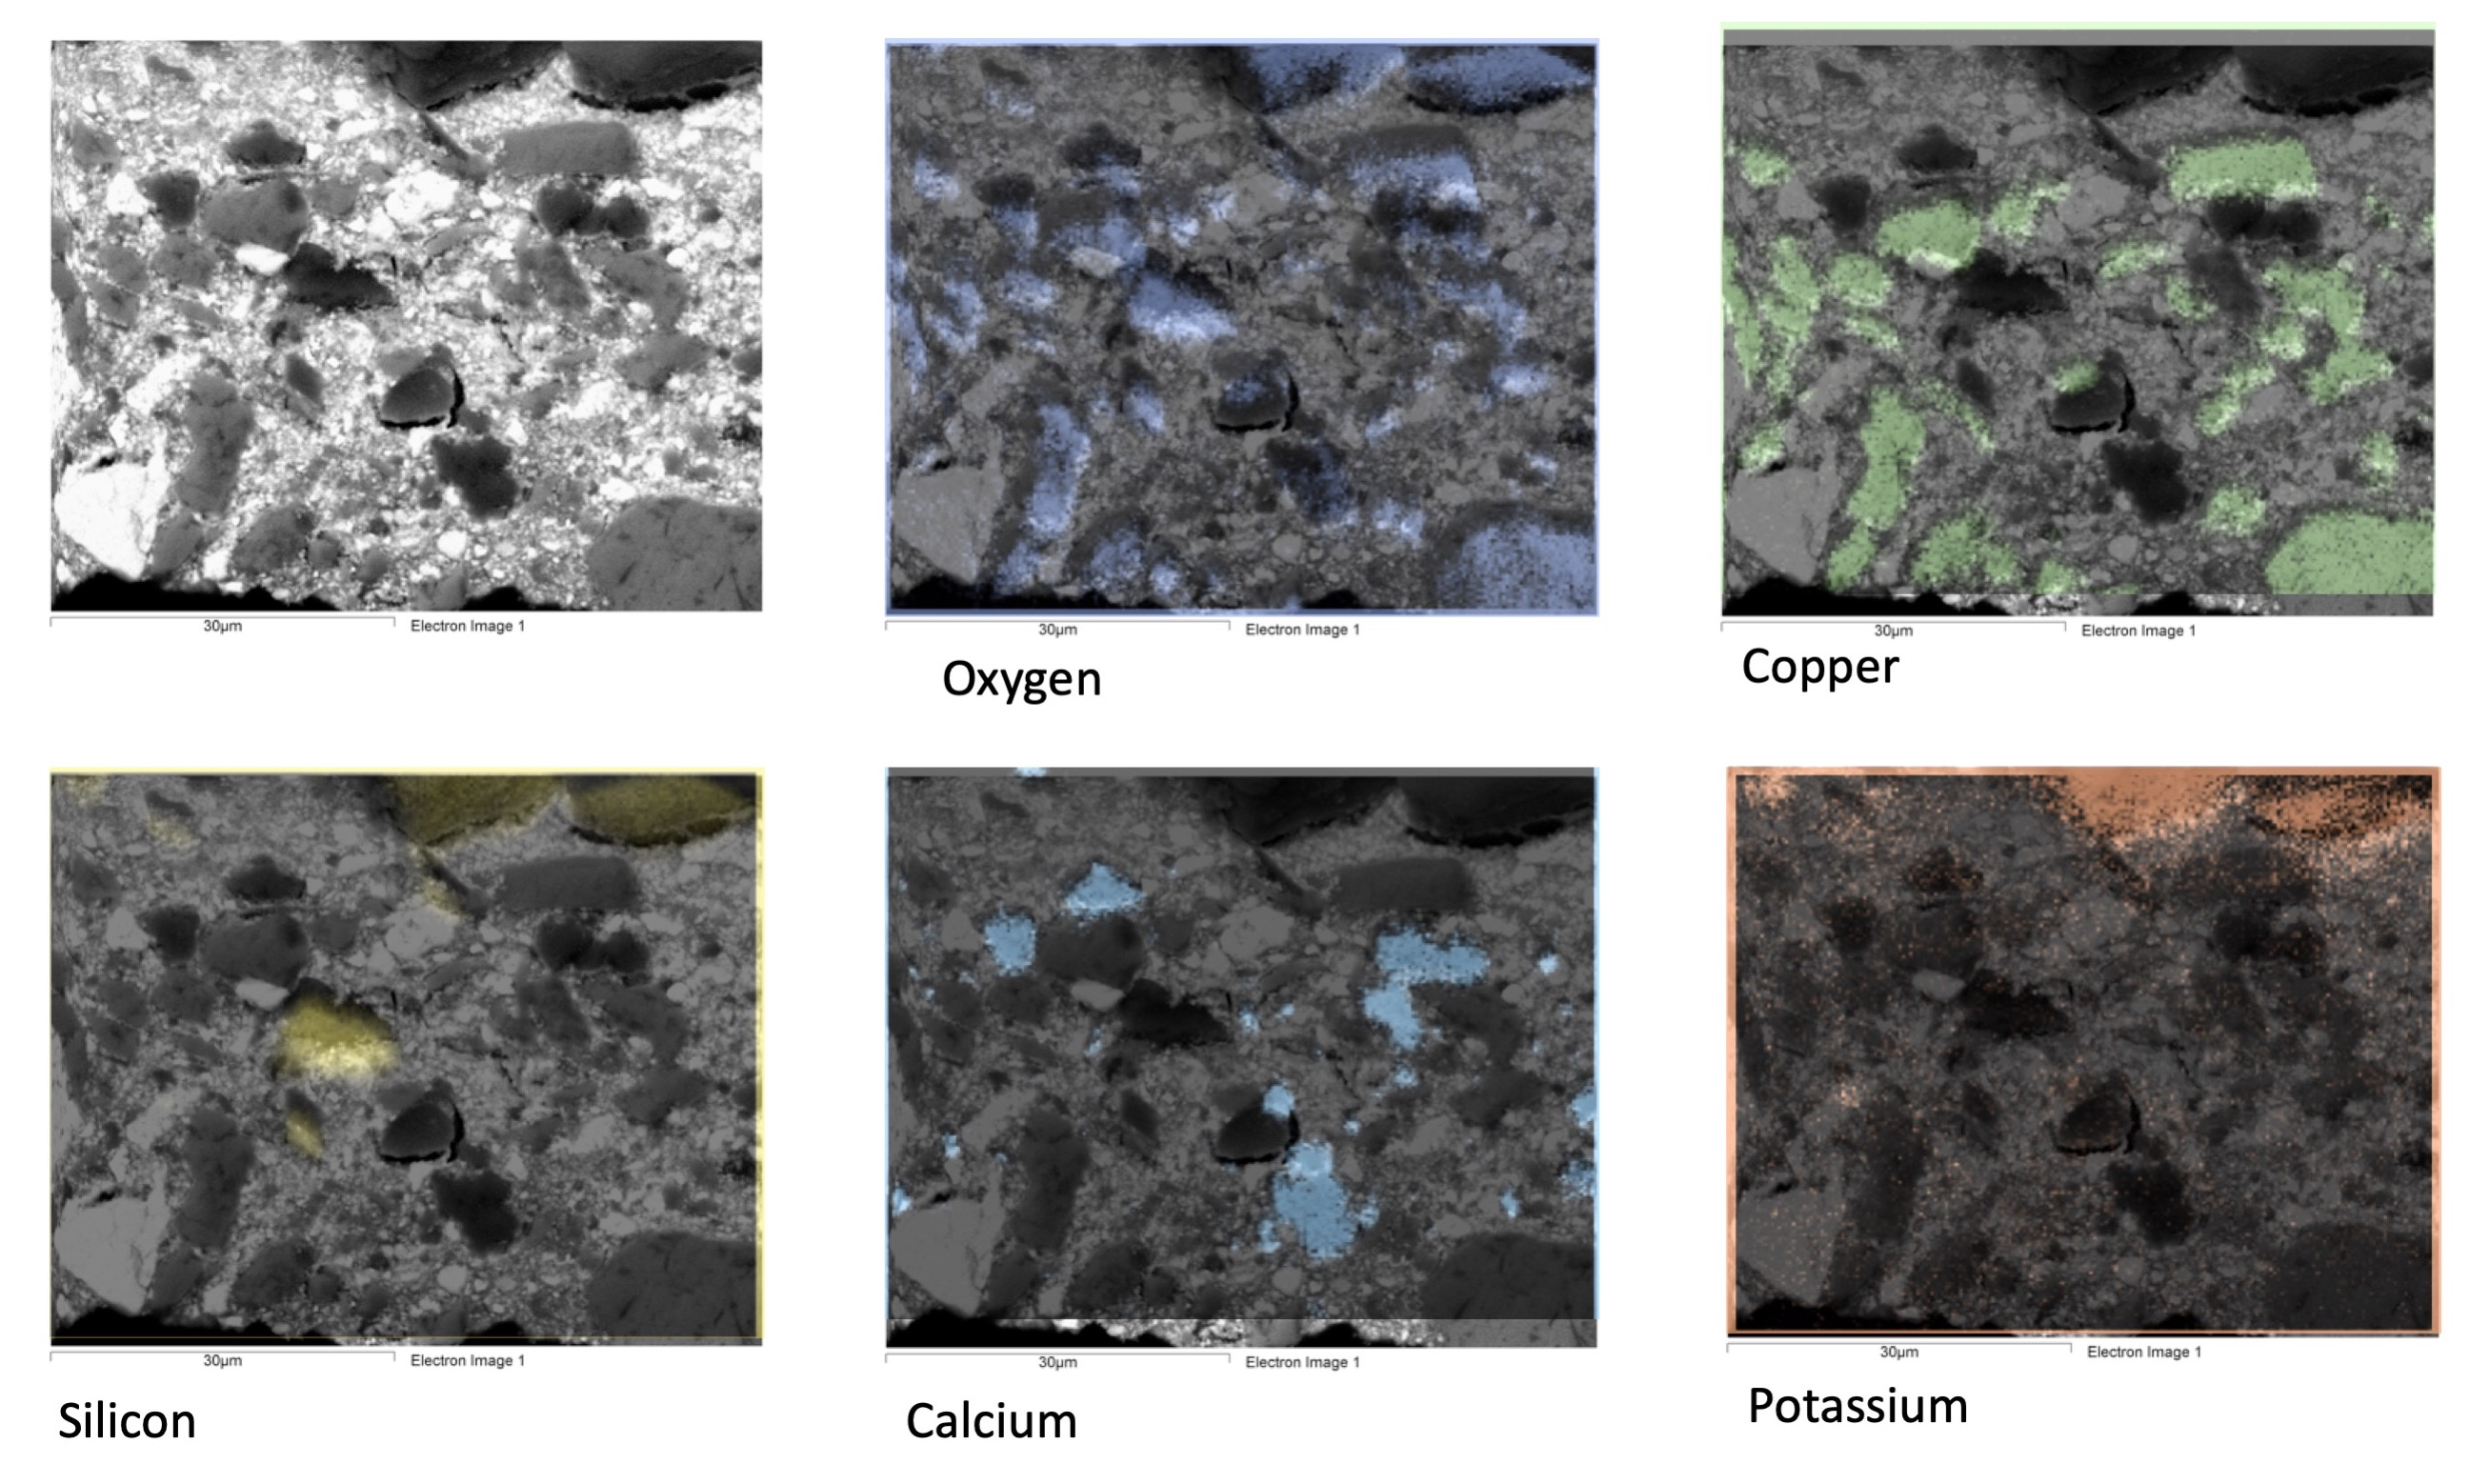
\includegraphics[width=0.9\linewidth]{1259-21_mapdata_1}
\hfill
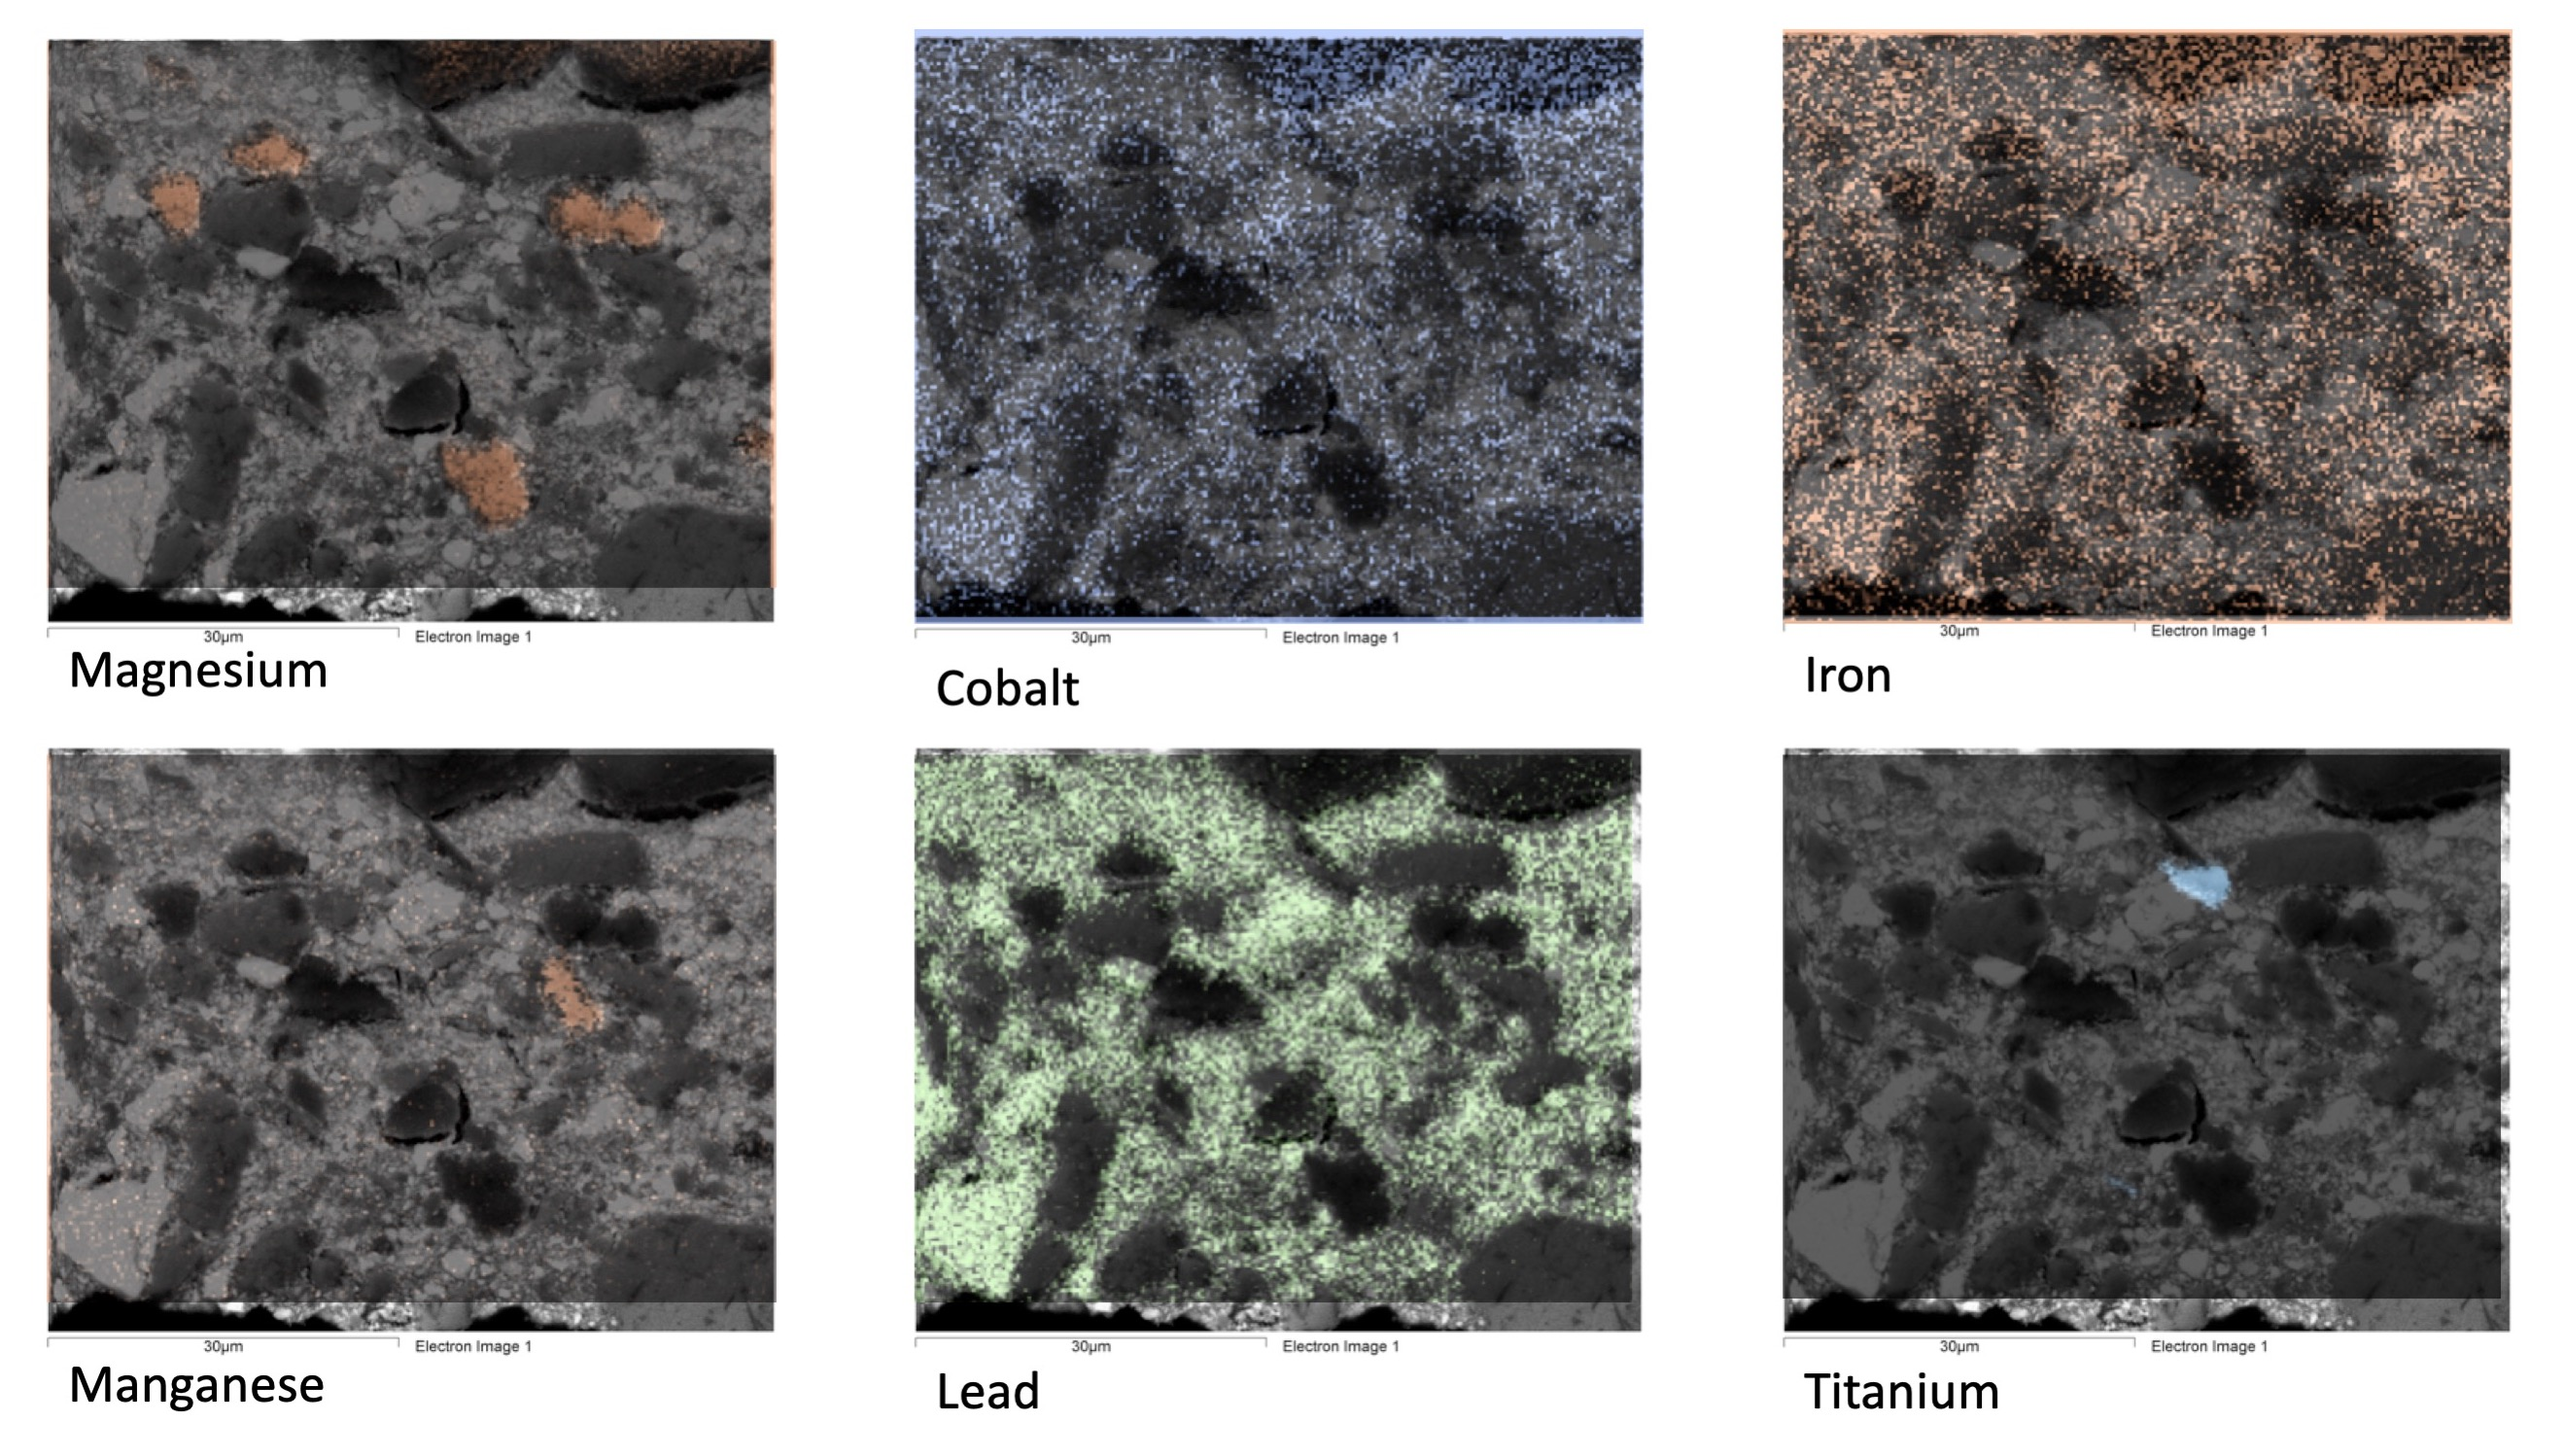
\includegraphics[width=0.9\linewidth]{1259-21_mapdata_2}
\hfill
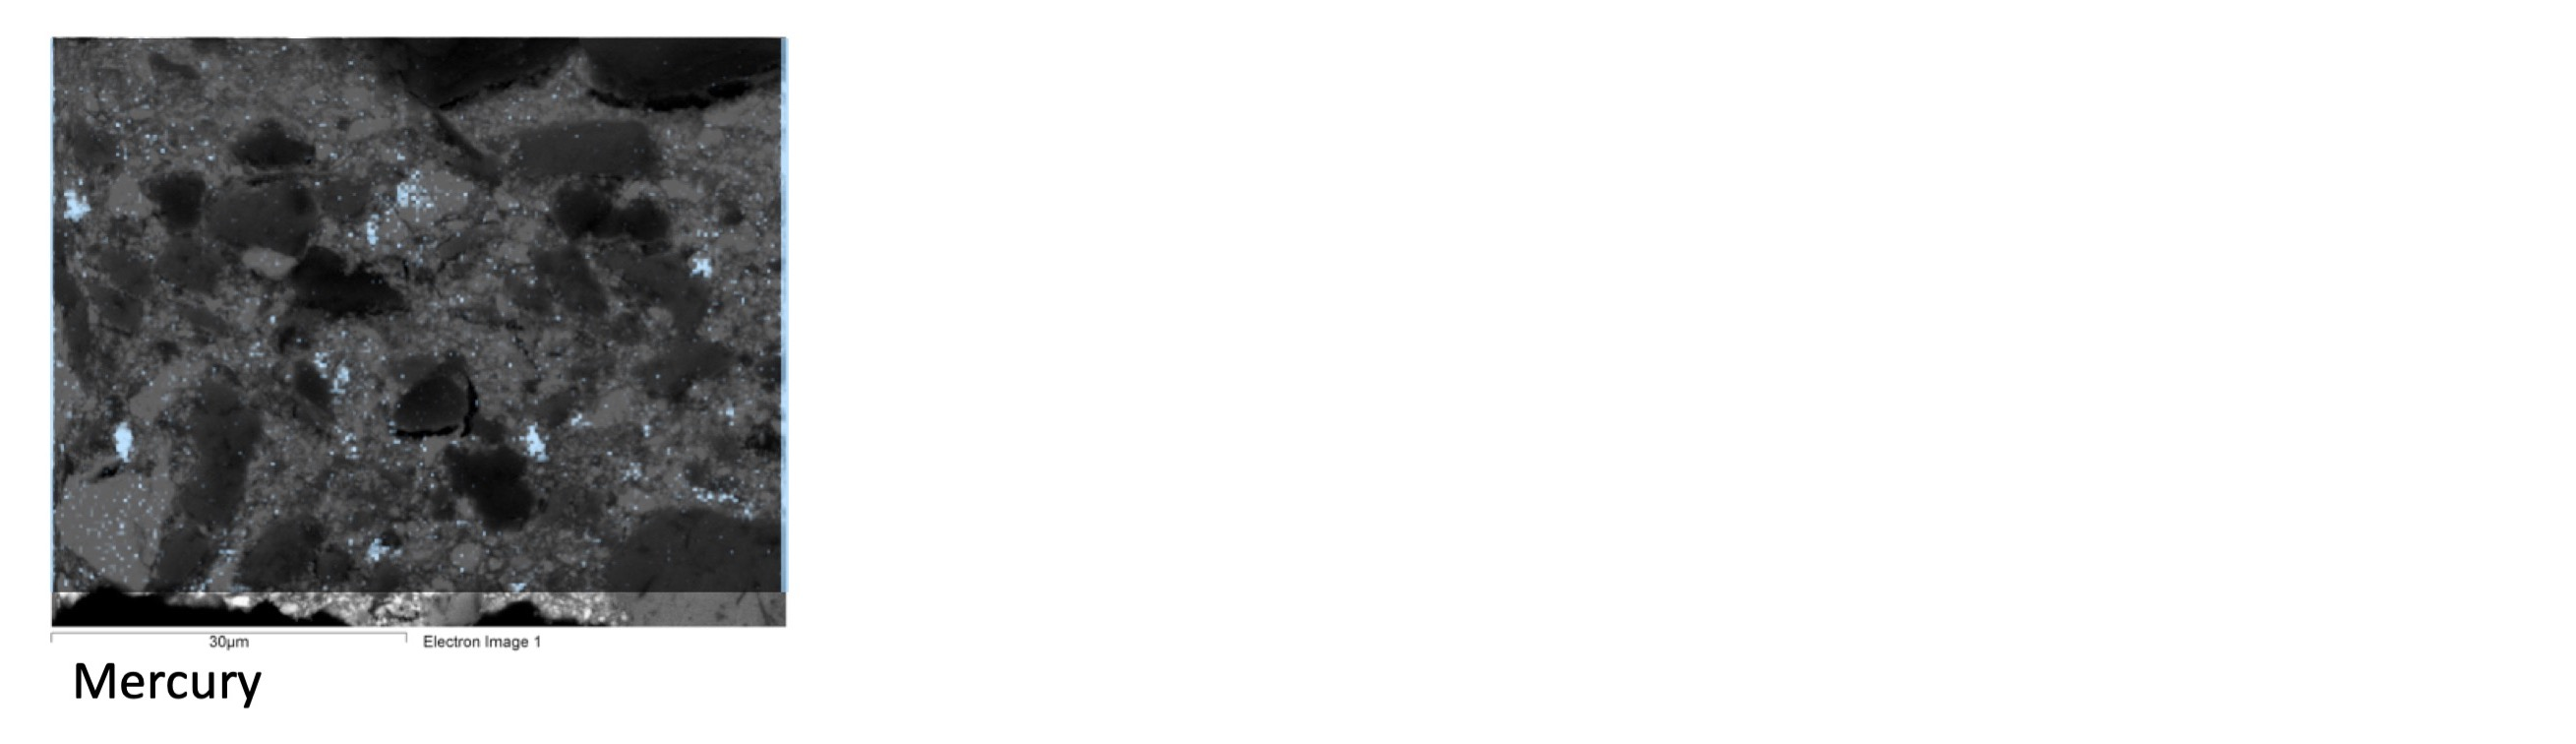
\includegraphics[width=0.9\linewidth]{1259-21_mapdata_3}
\hfill
\end{minipage}
\caption[EDS map data, sample 1259.21.]{EDS map data of sample 1259.21 showing locations of elements in an area of the azurite paint layer. Elements detected are O, Cu, Si, Ca, K, Mg, Co, Fe, Mn, Pb, Ti, and Hg.}
\label{fig:1259.21_mapdata}
\end{figure}


\begin{figure}[H]
\centering
  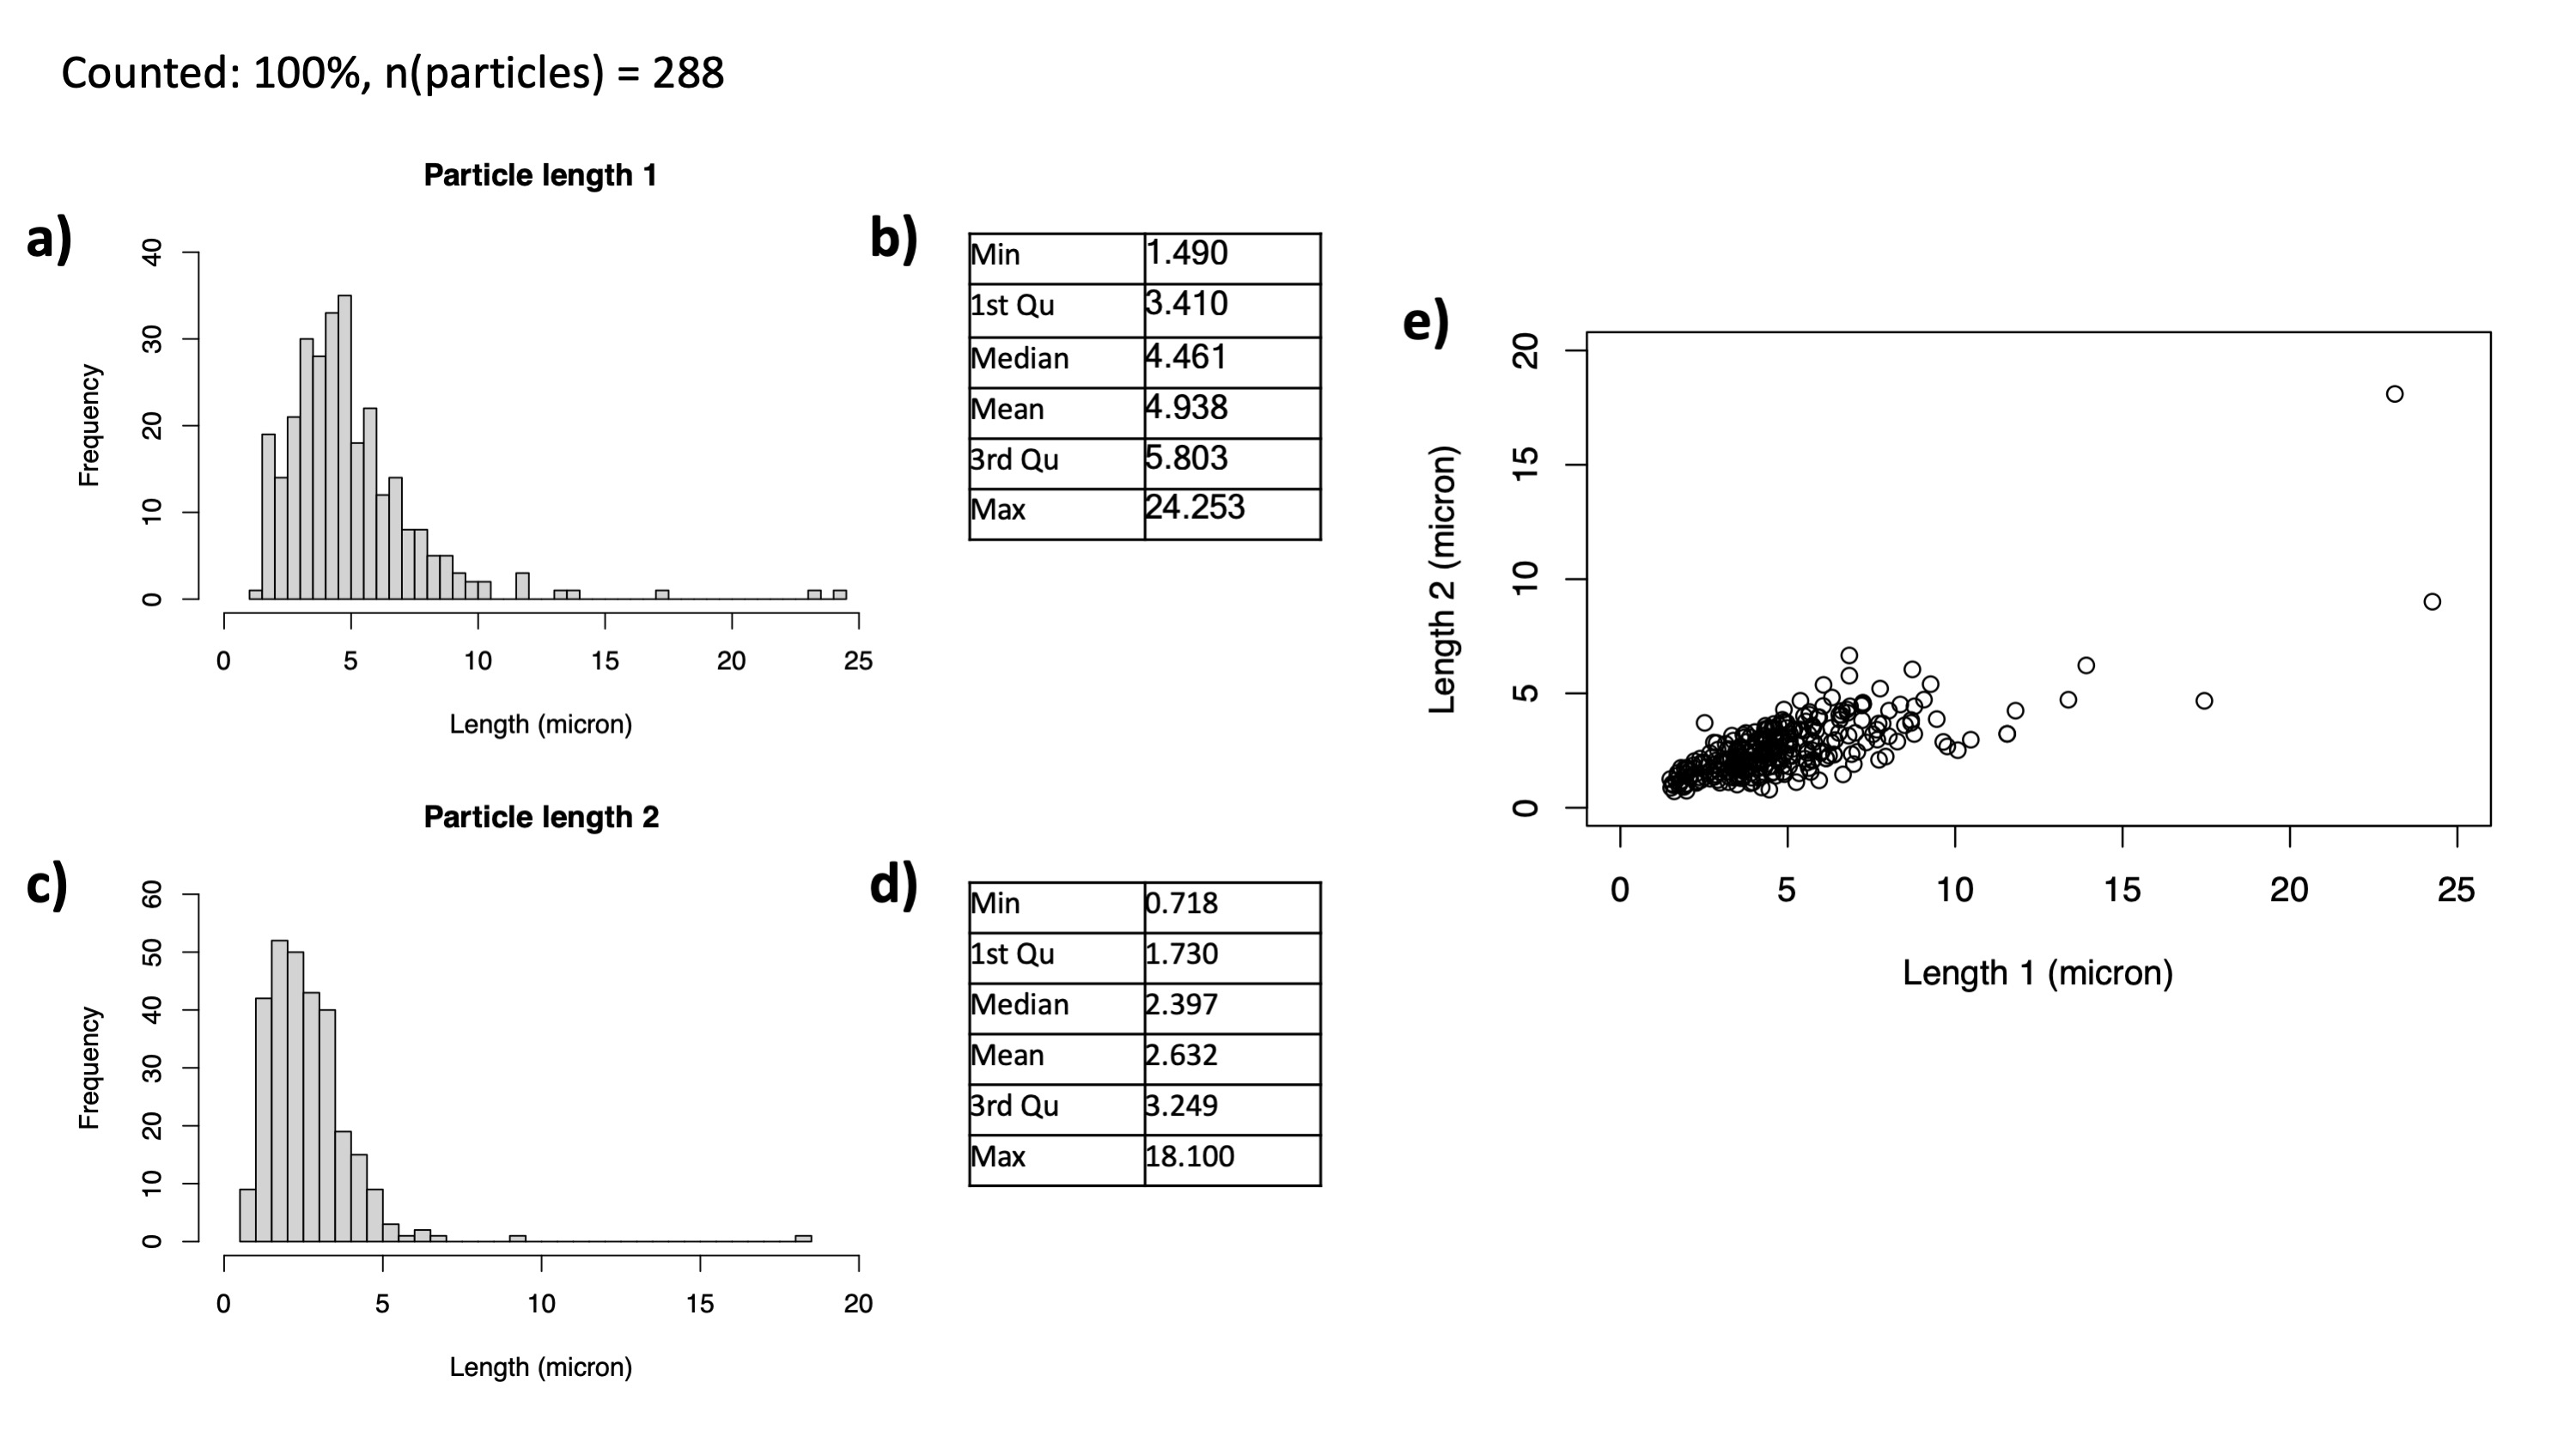
\includegraphics[width=\linewidth]{1259-21_partsize}
\caption[Particle size distribution, sample 1259.21.]{Particle size distribution of sample 1259.21: \textbf{a)} Histogram showing distribution of particle length 1 values. \textbf{b)} Descriptive statistics for particle length 1 data. \textbf{c)} Histogram showing distribution of particle length 2 values. \textbf{d)} Descriptive statistics for particle length 2 data. \textbf{e)} Graph of length 1 versus length 2 showing the degree of skew.}
\label{fig:1259.21_partsize}
\end{figure}


\section{Sample 1259.23}

\textit{Figure \ref{fig:1259.23_imgs}}, SEM and dark field images of 1259.23, shows a thick paint layer containing blue and white pigments, azurite and lead white. There are also red and yellow impurities in the dark field image, and the SEM images show a very heterogeneous mixture of particles as well. EDS map data (\textit{Figure \ref{fig:1259.23_mapdata}}) shows azurite and lead pigments, as well as dolomite and a silicon-containing component. Although map data shows localisation of zinc in the sample, this is an example of the danger of misinterpreting overlapped peaks; the zinc and copper locations are the same, and it is far more likely that the detection of zinc is actually due to copper. Particle size data, presented in \textit{Figure \ref{fig:1259.23_partsize}}, shows a low concentration of azurite particles and relatively high skew.


\begin{figure}[H]
  \centering
  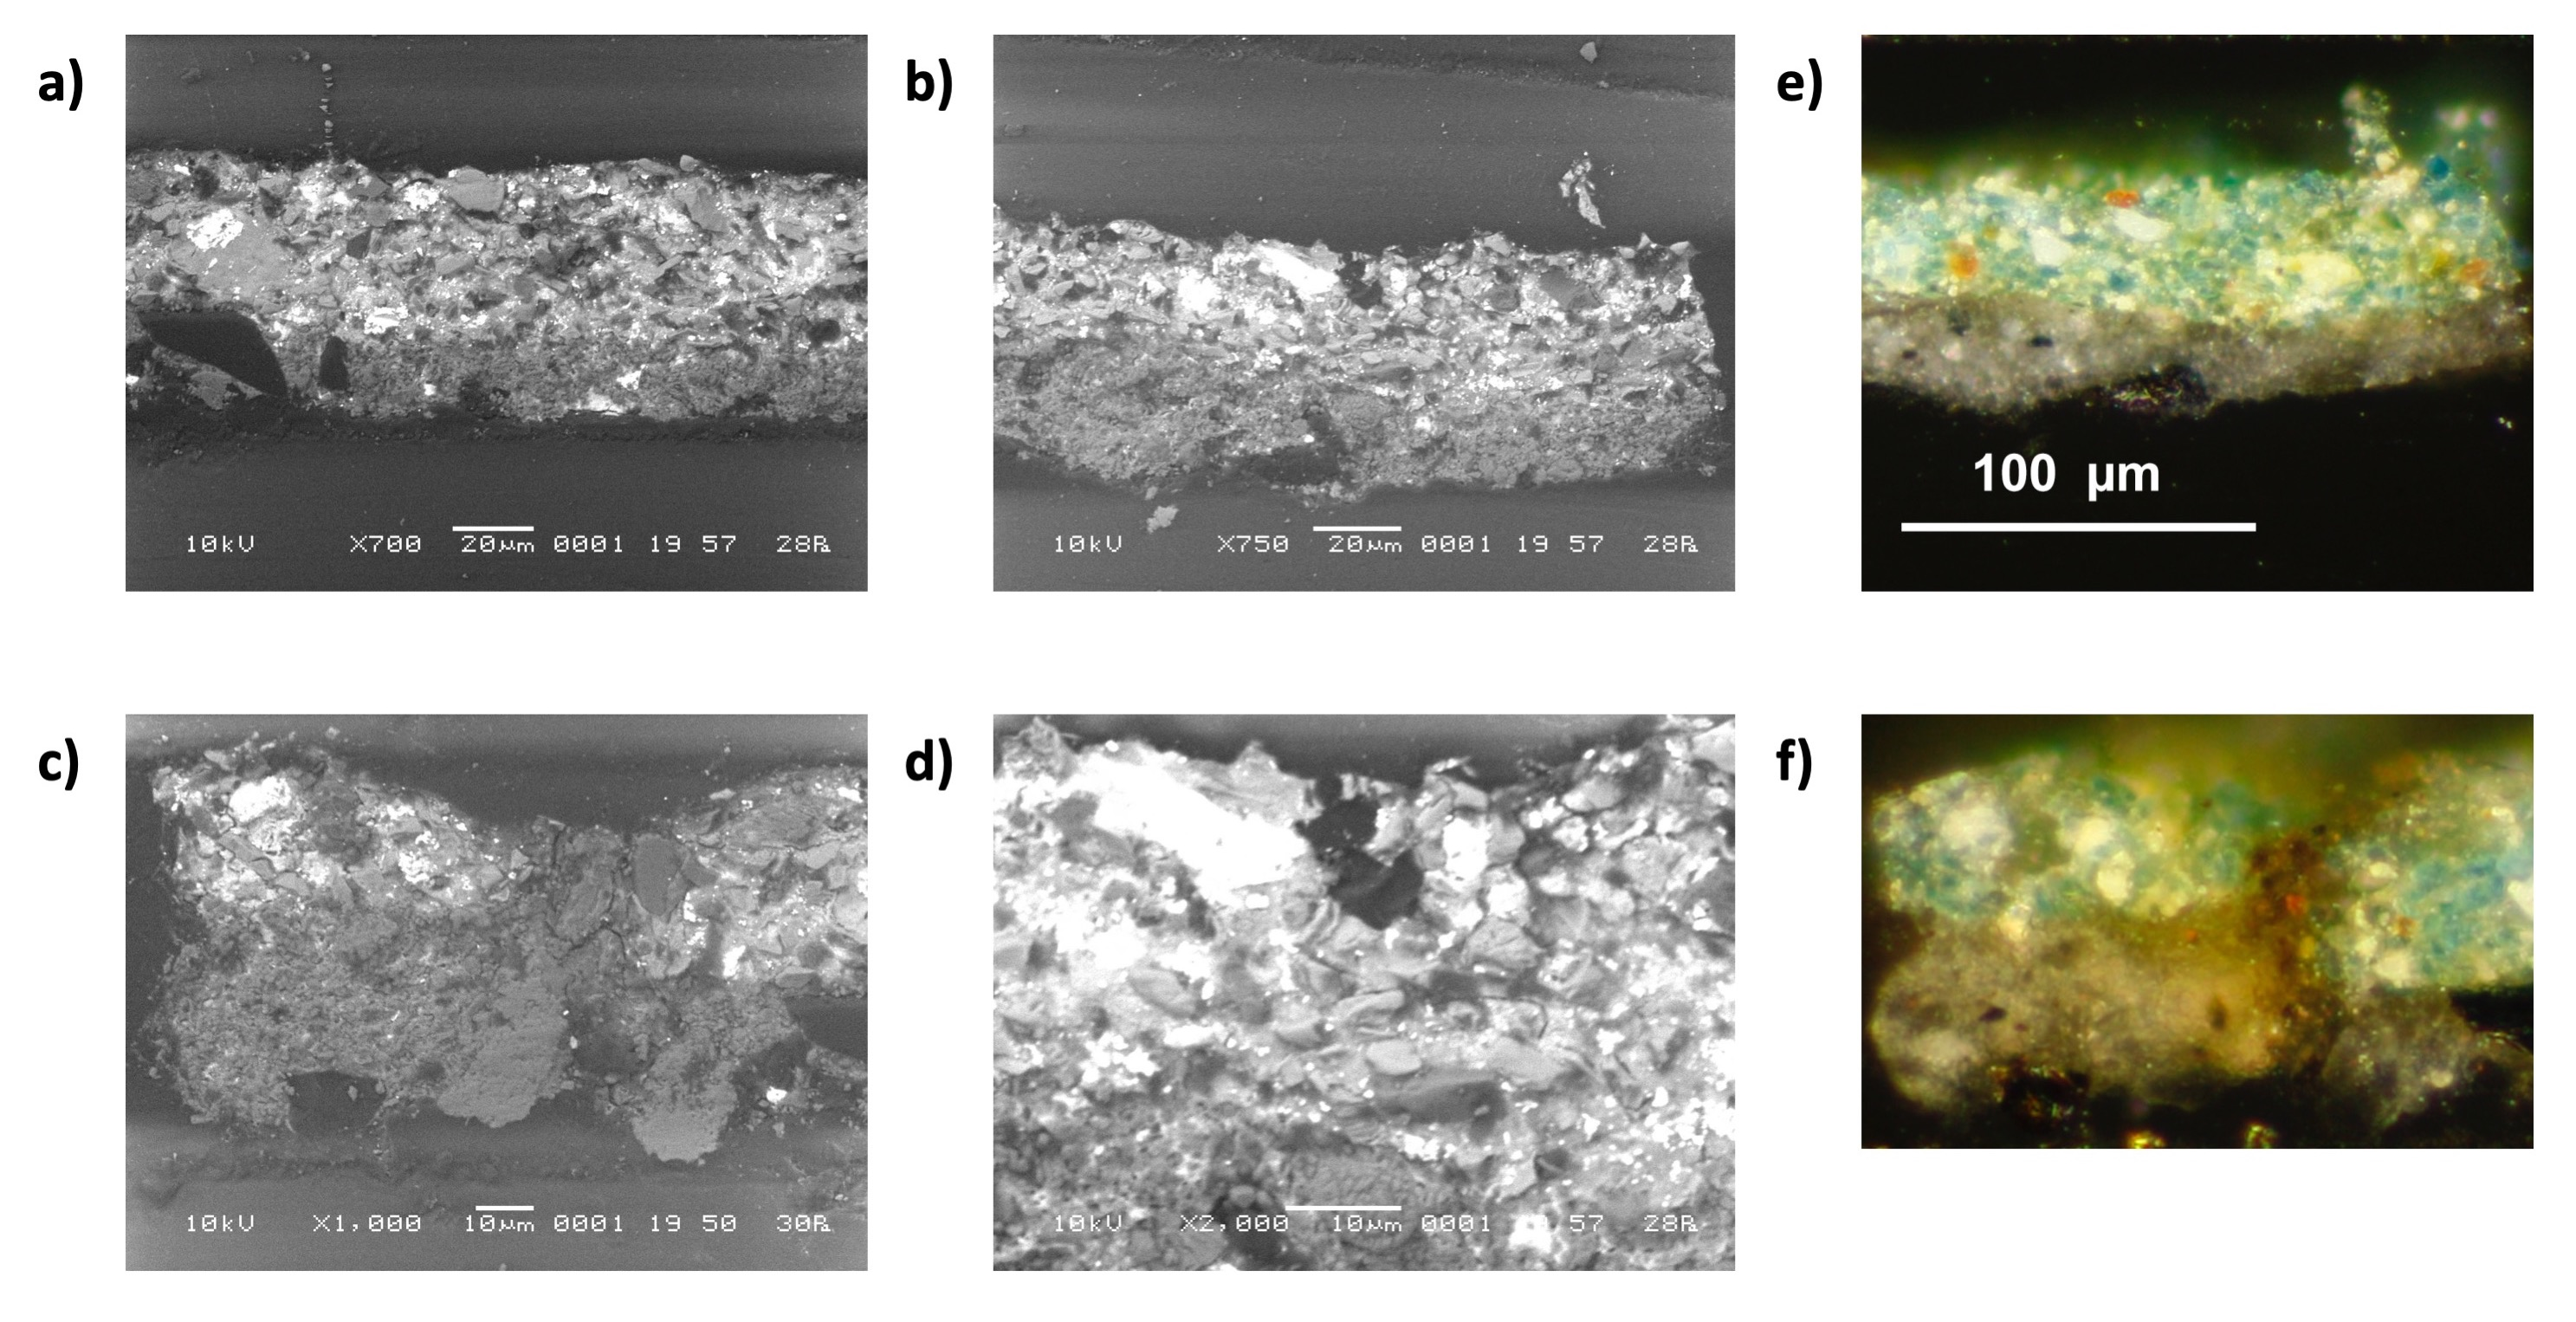
\includegraphics[width=\linewidth]{1259-23_imgs}
\caption[SEM and dark field images of sample 1259.21.]{SEM and dark field images of sample 1259.21: \textbf{a)} 700x magnification, \textbf{b)} 750x magnification, \textbf{c)} 1000x magnification, \textbf{d)} 2000x magnification, \textbf{e)} and \textbf{f)}, dark field microscope images corresponding to \textbf{b} and \textbf{c} respectively. Dark field microscope images courtesy of Katharine Waldron, HKI.}
\label{fig:1259.23_imgs}
\end{figure}

\begin{figure}[H]
  \centering
  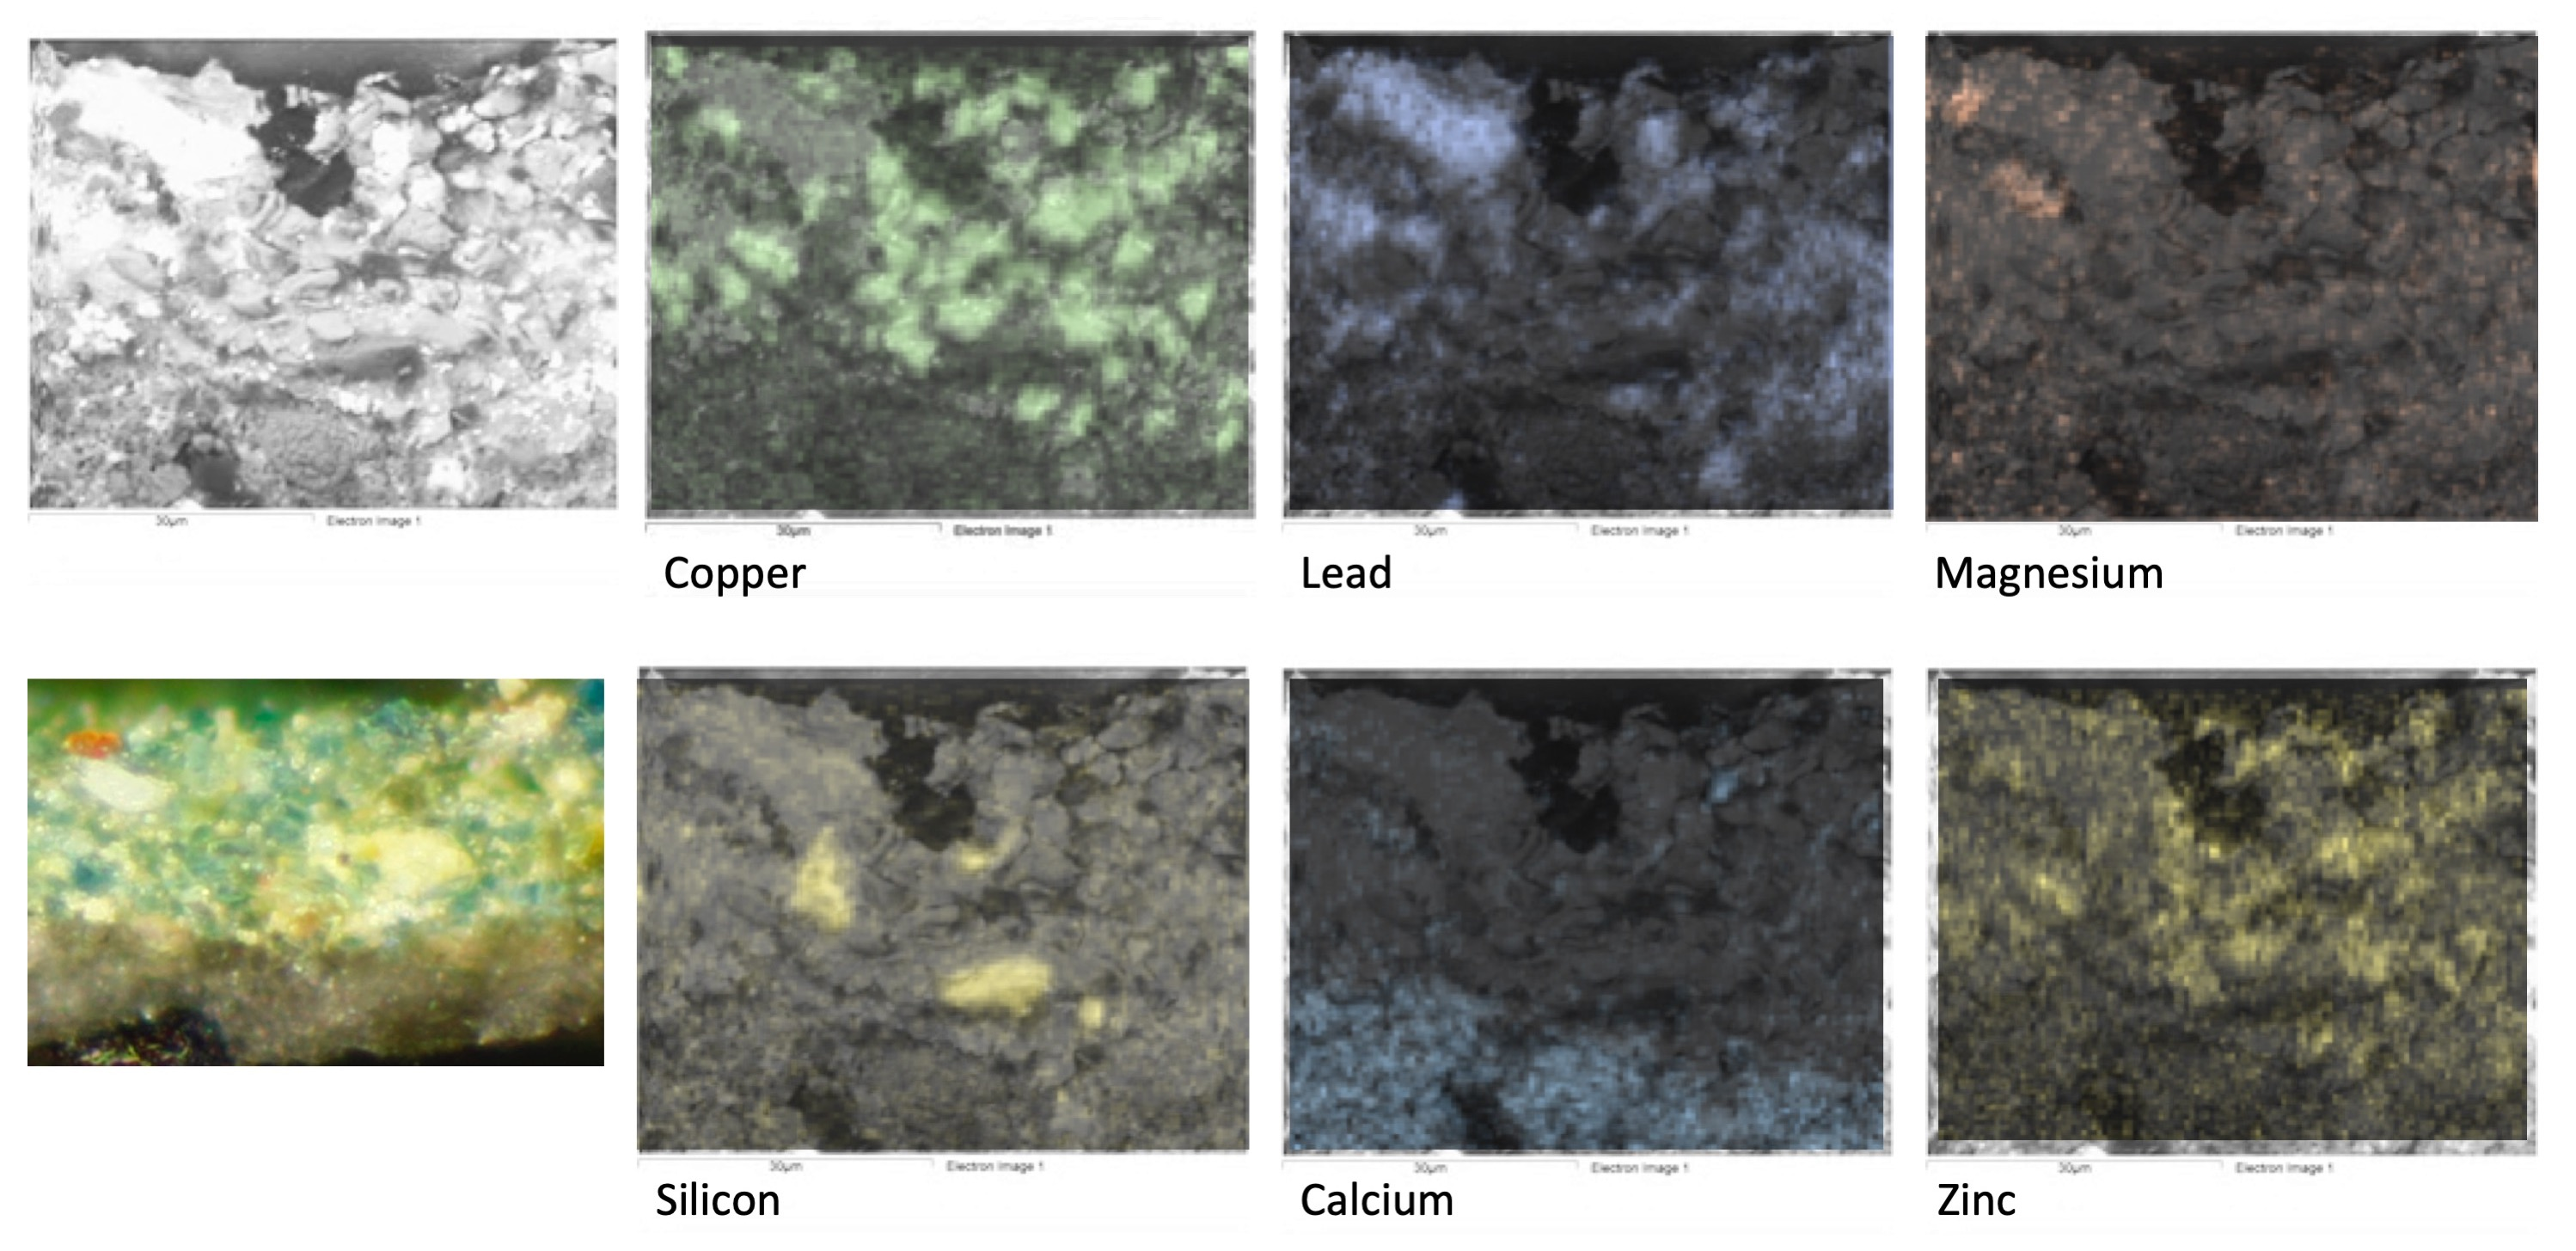
\includegraphics[width=0.9\linewidth]{1259-23_mapdata}
\caption[EDS map data, sample 1259.23.]{EDS map data of sample 1259.23 showing locations of elements in an area of the azurite paint layer. Elements detected are Cu, Pb, Mg, Si, Ca, Zn. SEM and dark field microscope images of mapped area are also shown. The dark field microscope image is provided by Katharine Waldron, HKI.}
\label{fig:1259.23_mapdata}
\end{figure}


\begin{figure}[H]
\centering
  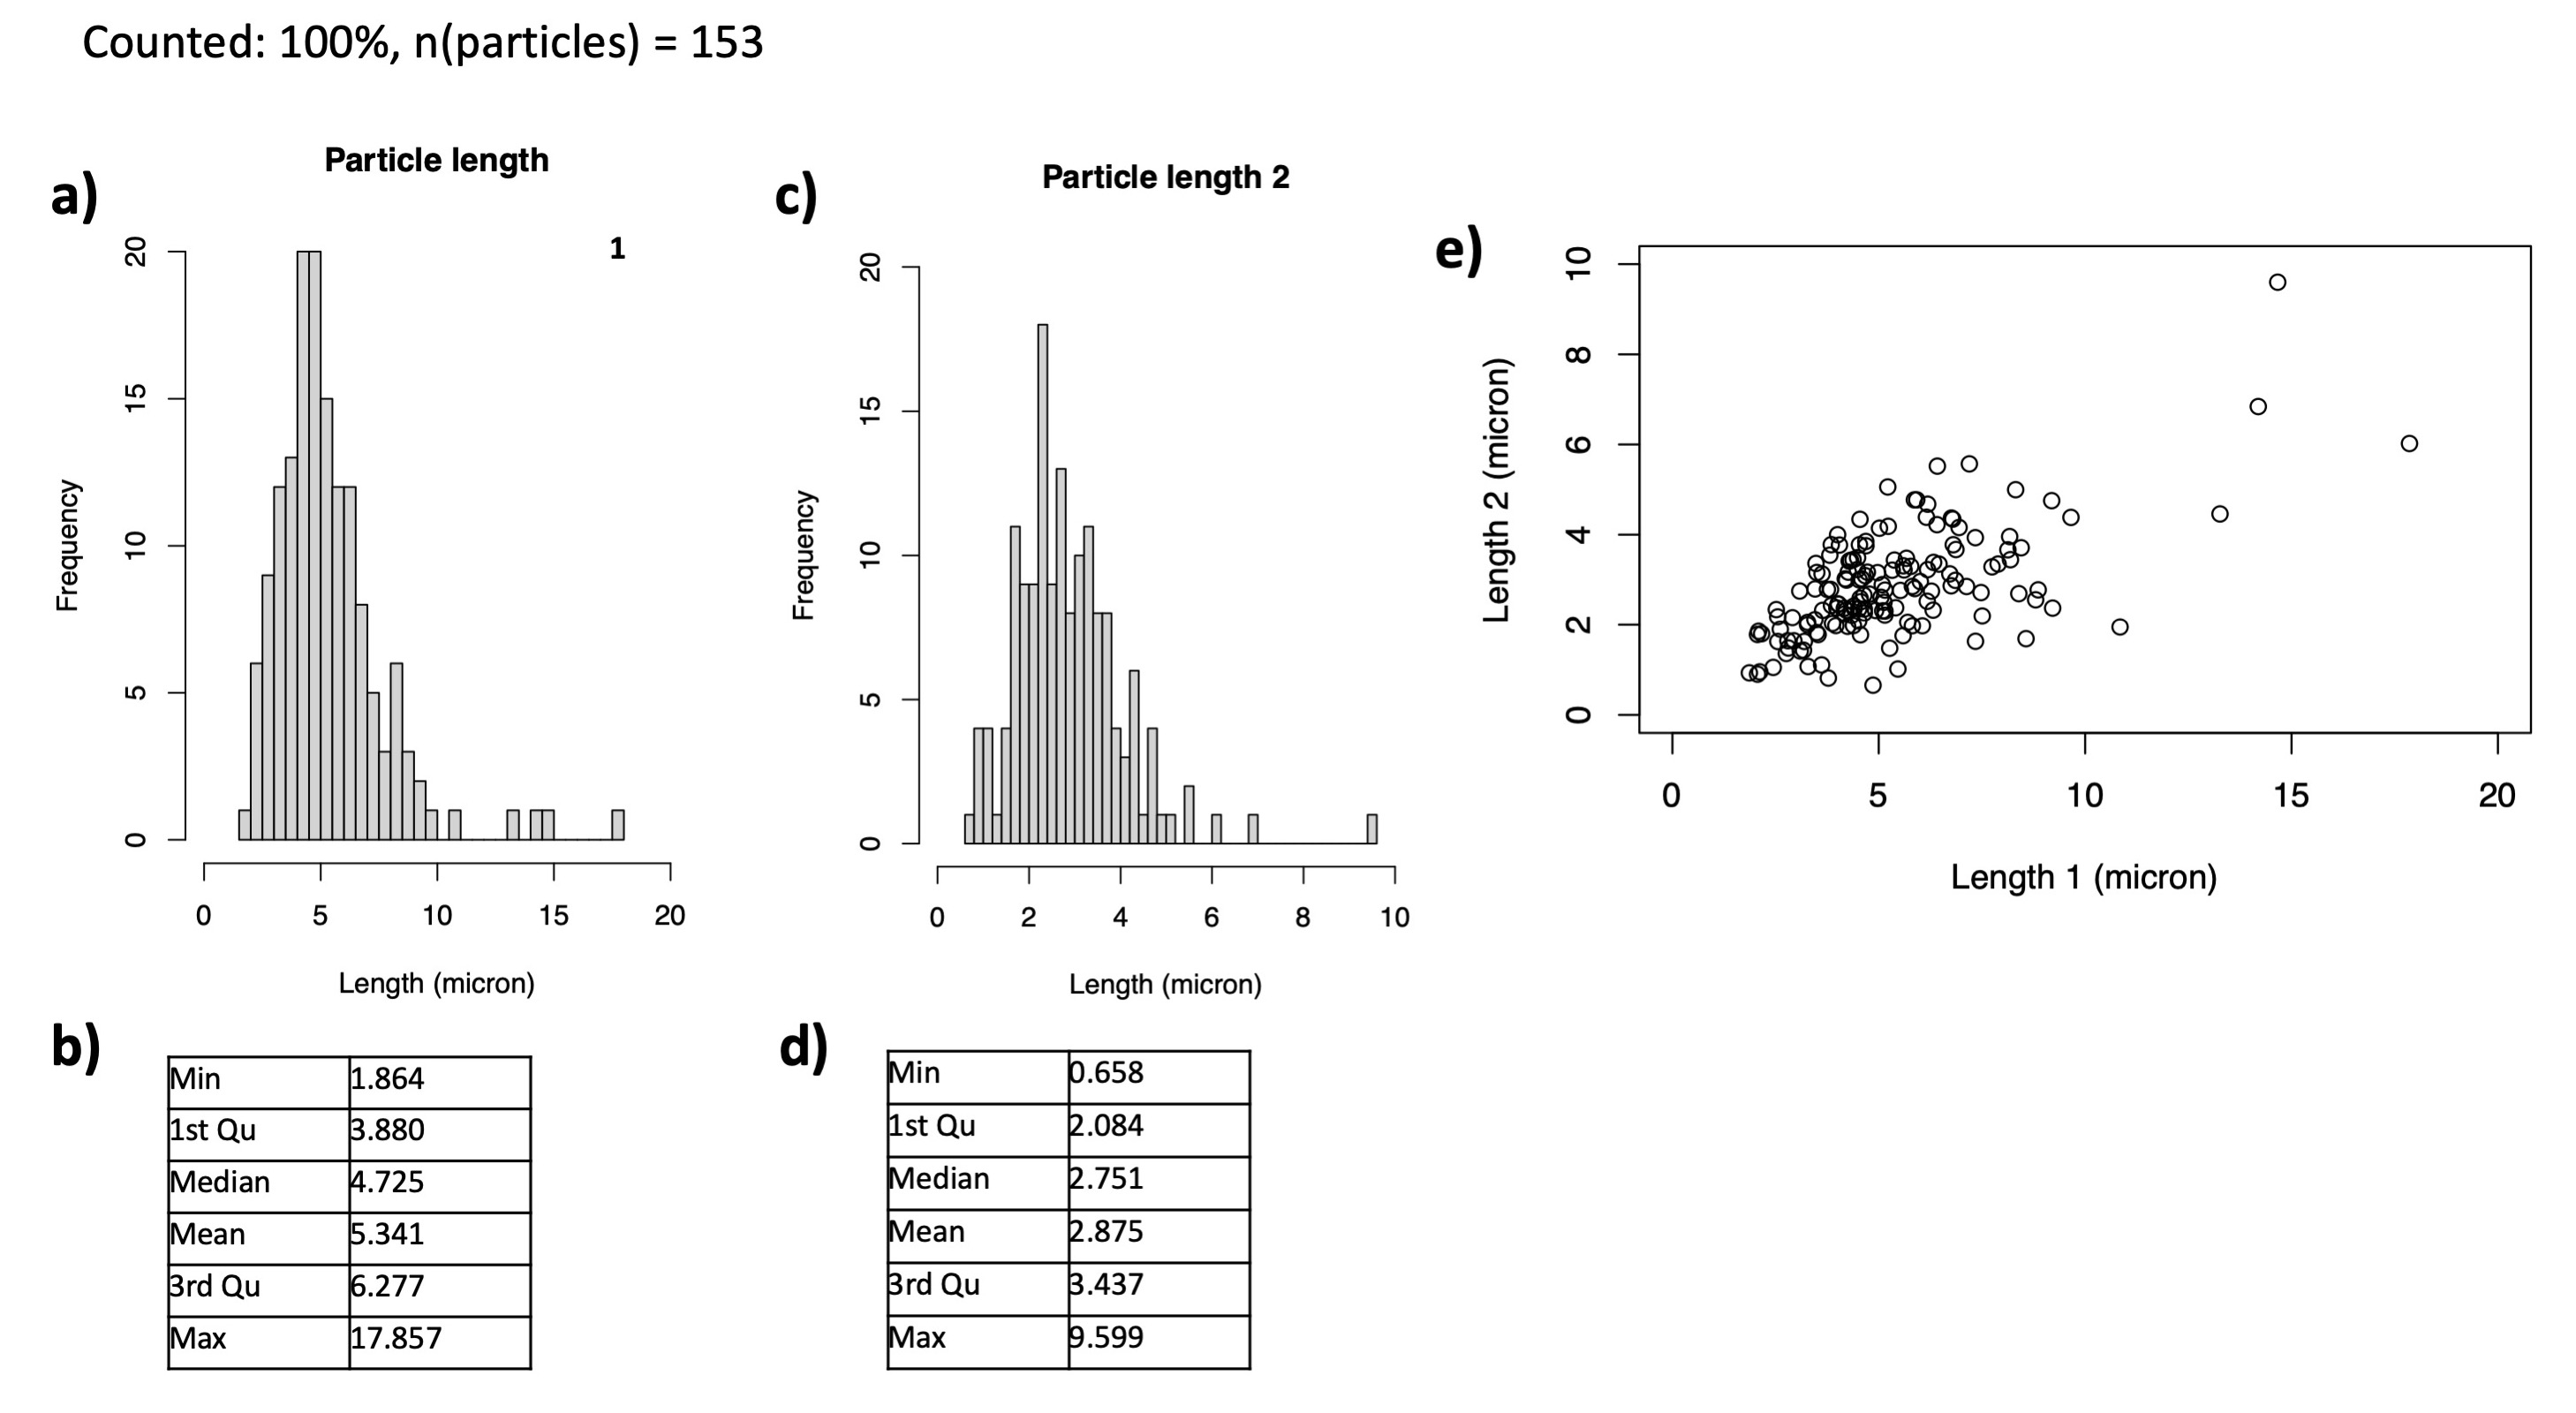
\includegraphics[width=\linewidth]{1259-23_partsize}
\caption[Particle size distribution, sample 1259.23.]{Particle size distribution of sample 1259.23: \textbf{a)} Histogram showing distribution of particle length 1 values. \textbf{b)} Descriptive statistics for particle length 1 data. \textbf{c)} Histogram showing distribution of particle length 2 values. \textbf{d)} Descriptive statistics for particle length 2 data. \textbf{e)} Graph of length 1 versus length 2 showing the degree of skew.}
\label{fig:1259.23_partsize}
\end{figure}



\section{Sample 1259.28}

SEM/dark field images of 1259.28 (\textit{Figure \ref{fig:1259.28_imgs}}) show a thin upper layer of dense azurite particles with primarily white and red impurities. EDS confirms the red particles as iron oxide (\textit{Figure \ref{fig:1259.28_map_iron}}). Element maps are shown in \textit{Figure \ref{fig:1259.28_mapdata}}, confirming azurite, aluminosilicates, dolomite, and a lead containing compound. Interestingly, point spectra of the lead material (\textit{Figure \ref{fig:1259.28_pointspec}}) also shows high levels of tin. Lead-tin yellow is a historical pigment that is accurate to the time period, but the sample does not show yellow particles in the dark field image. This is an interesting result that may be expored further. \textit{Figure \ref{fig:1259.28_partsize}} shows a wide distribution of particle dimensions and a larger difference between the mean and median length values than that of other samples analysed.

\begin{figure}[H]
  \centering
  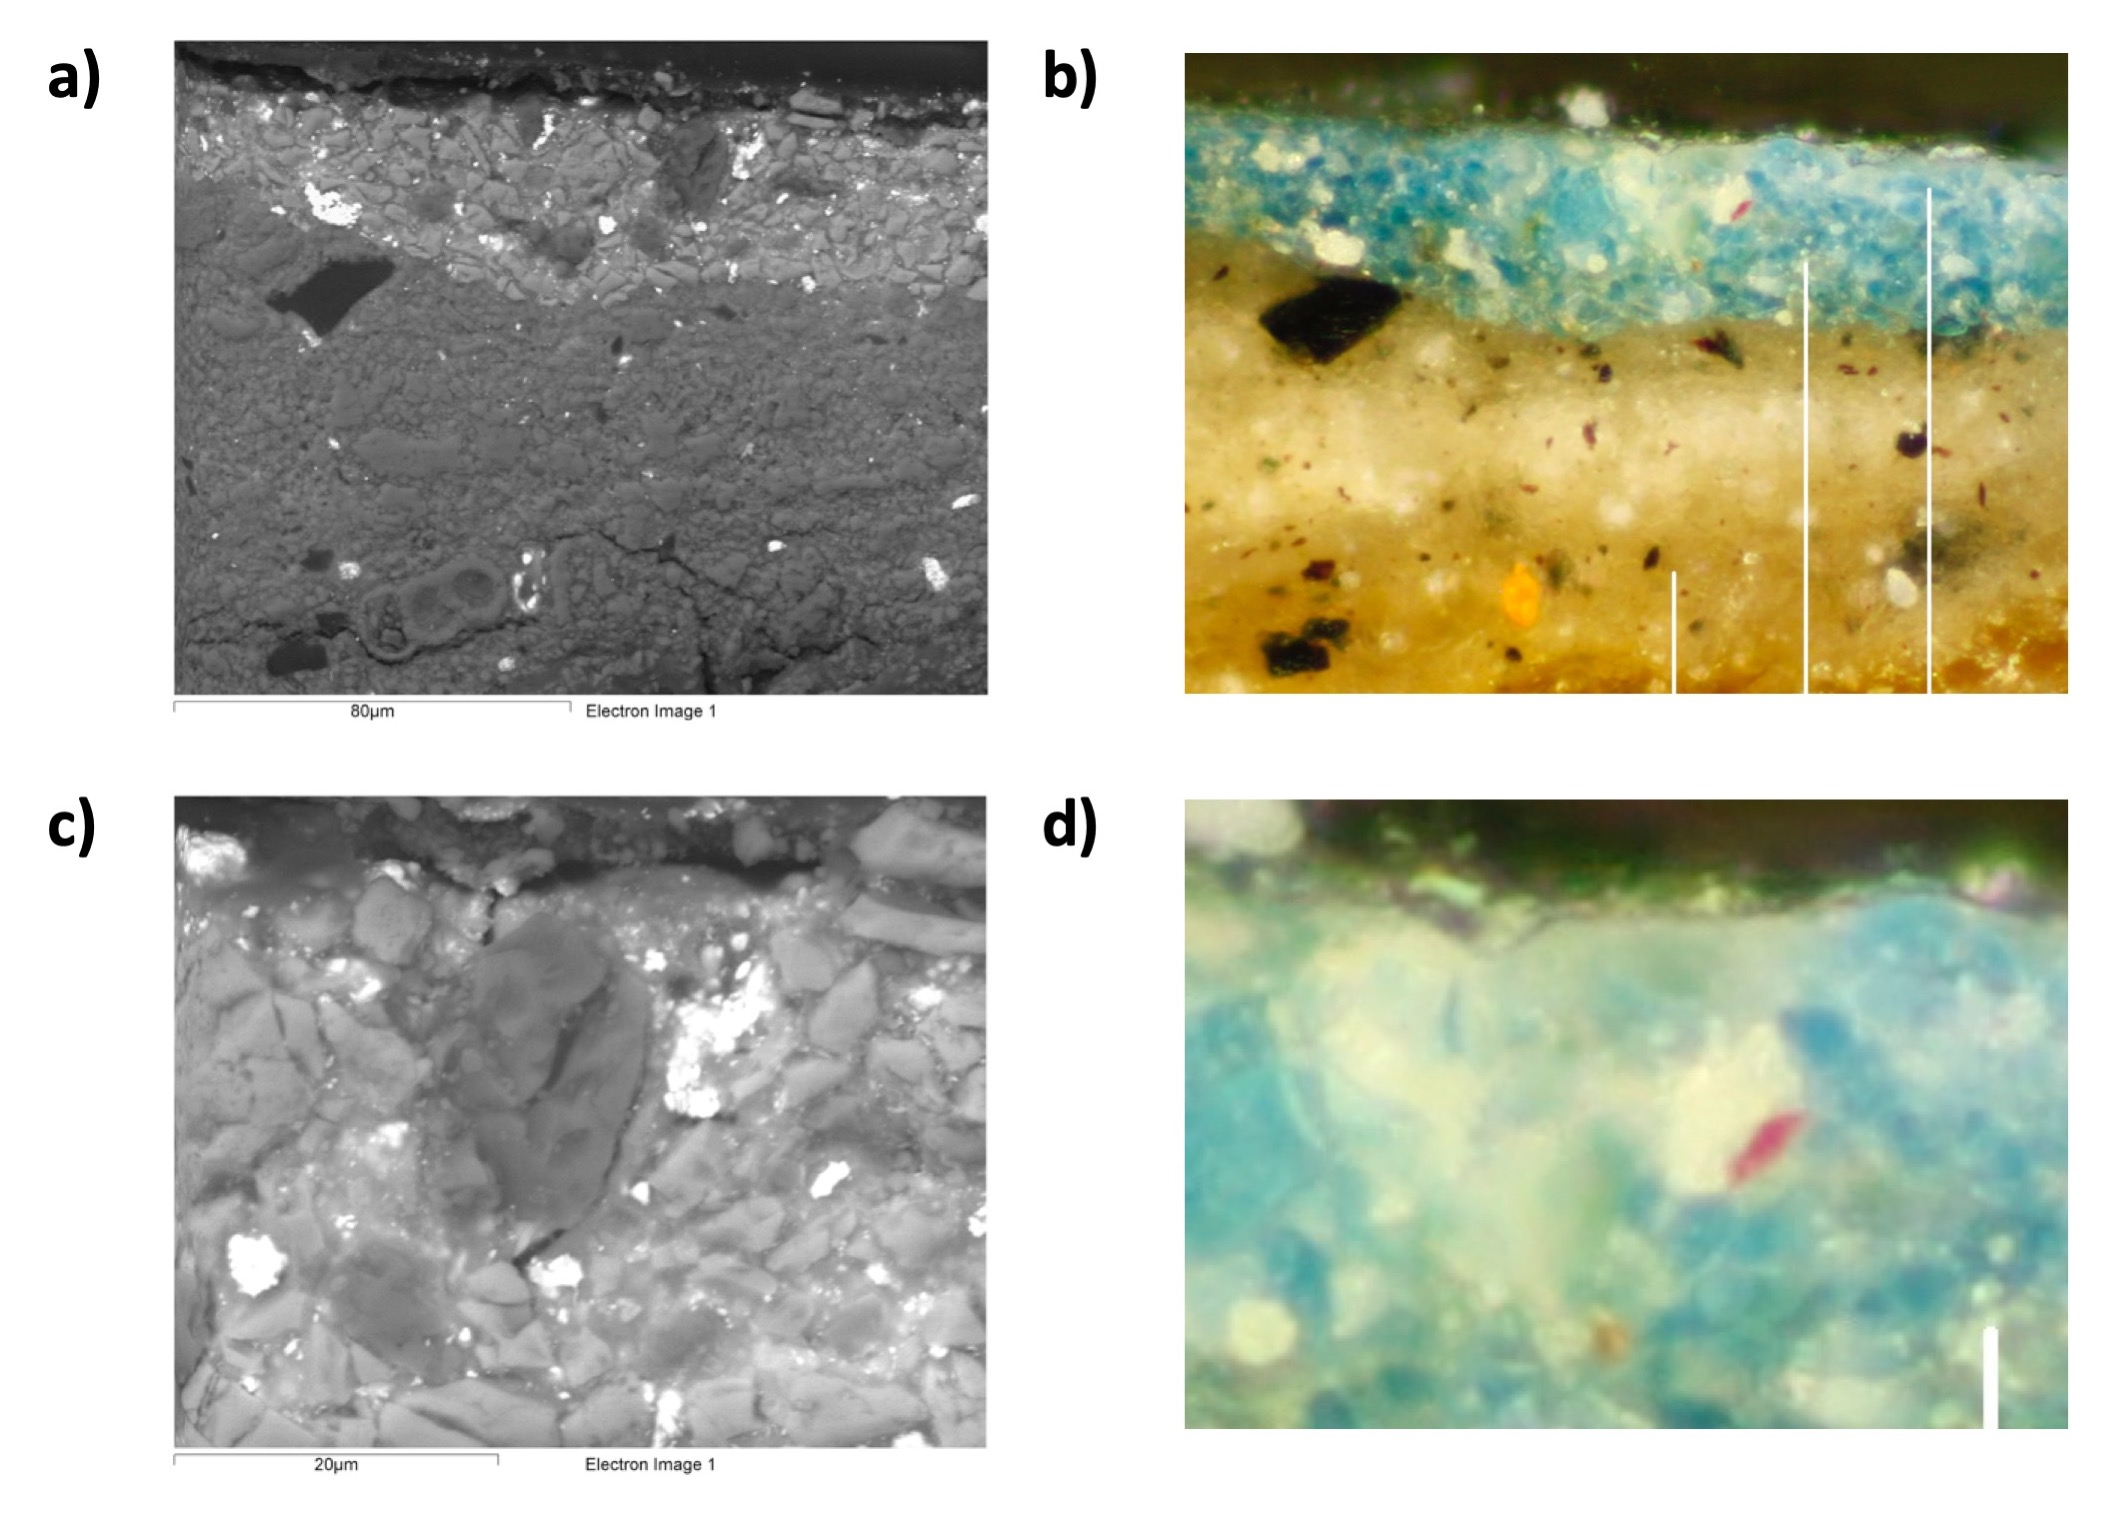
\includegraphics[width=\linewidth]{1259-28_imgs}
\caption[SEM and dark field images of sample 1259.28.]{SEM and dark field images of sample 1259.28: \textbf{a)} 750x magnification, \textbf{b)} corresponding dark field microscope image, \textbf{c)} 2000x magnification, \textbf{d)} corresponding dark field microscope image. Dark field microscope images courtesy of Katharine Waldron, HKI.}
\label{fig:1259.28_imgs}
\end{figure}

\begin{figure}[H]
  \centering
  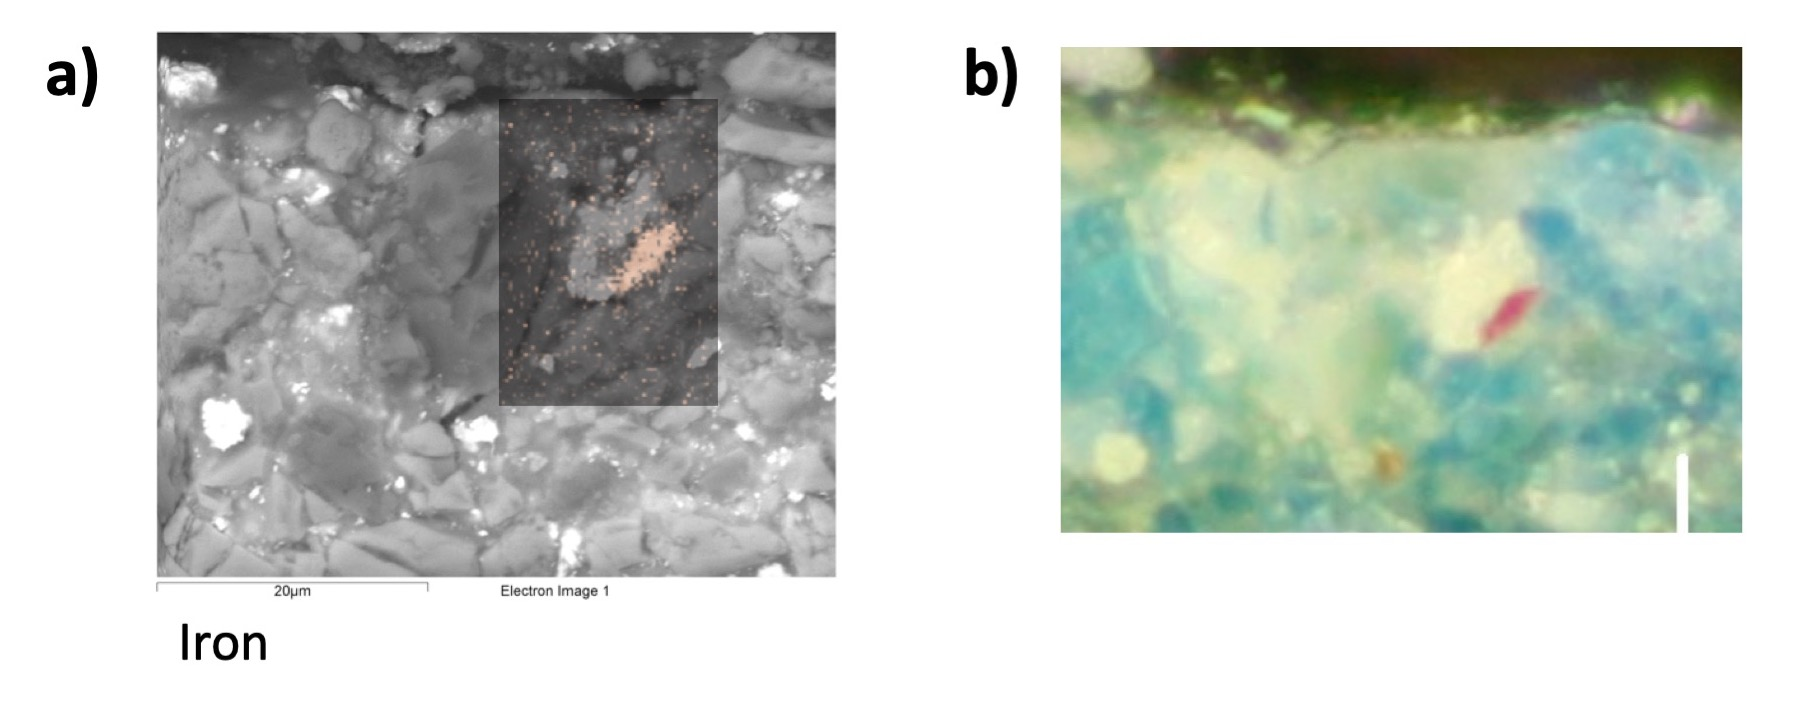
\includegraphics[width=\linewidth]{1259-28_map_iron}
\caption[EDS map data, sample 1259.28.]{EDS map data, sample 1259.28: \textbf{a)} Fe overlay on SEM image, \textbf{b)} Dark field microscope image showing same area including red iron oxide particle. Image is provided courtesy of Katharine Waldron, HKI.}
\label{fig:1259.28_map_iron}
\end{figure}


\begin{figure}[H]
  \centering
  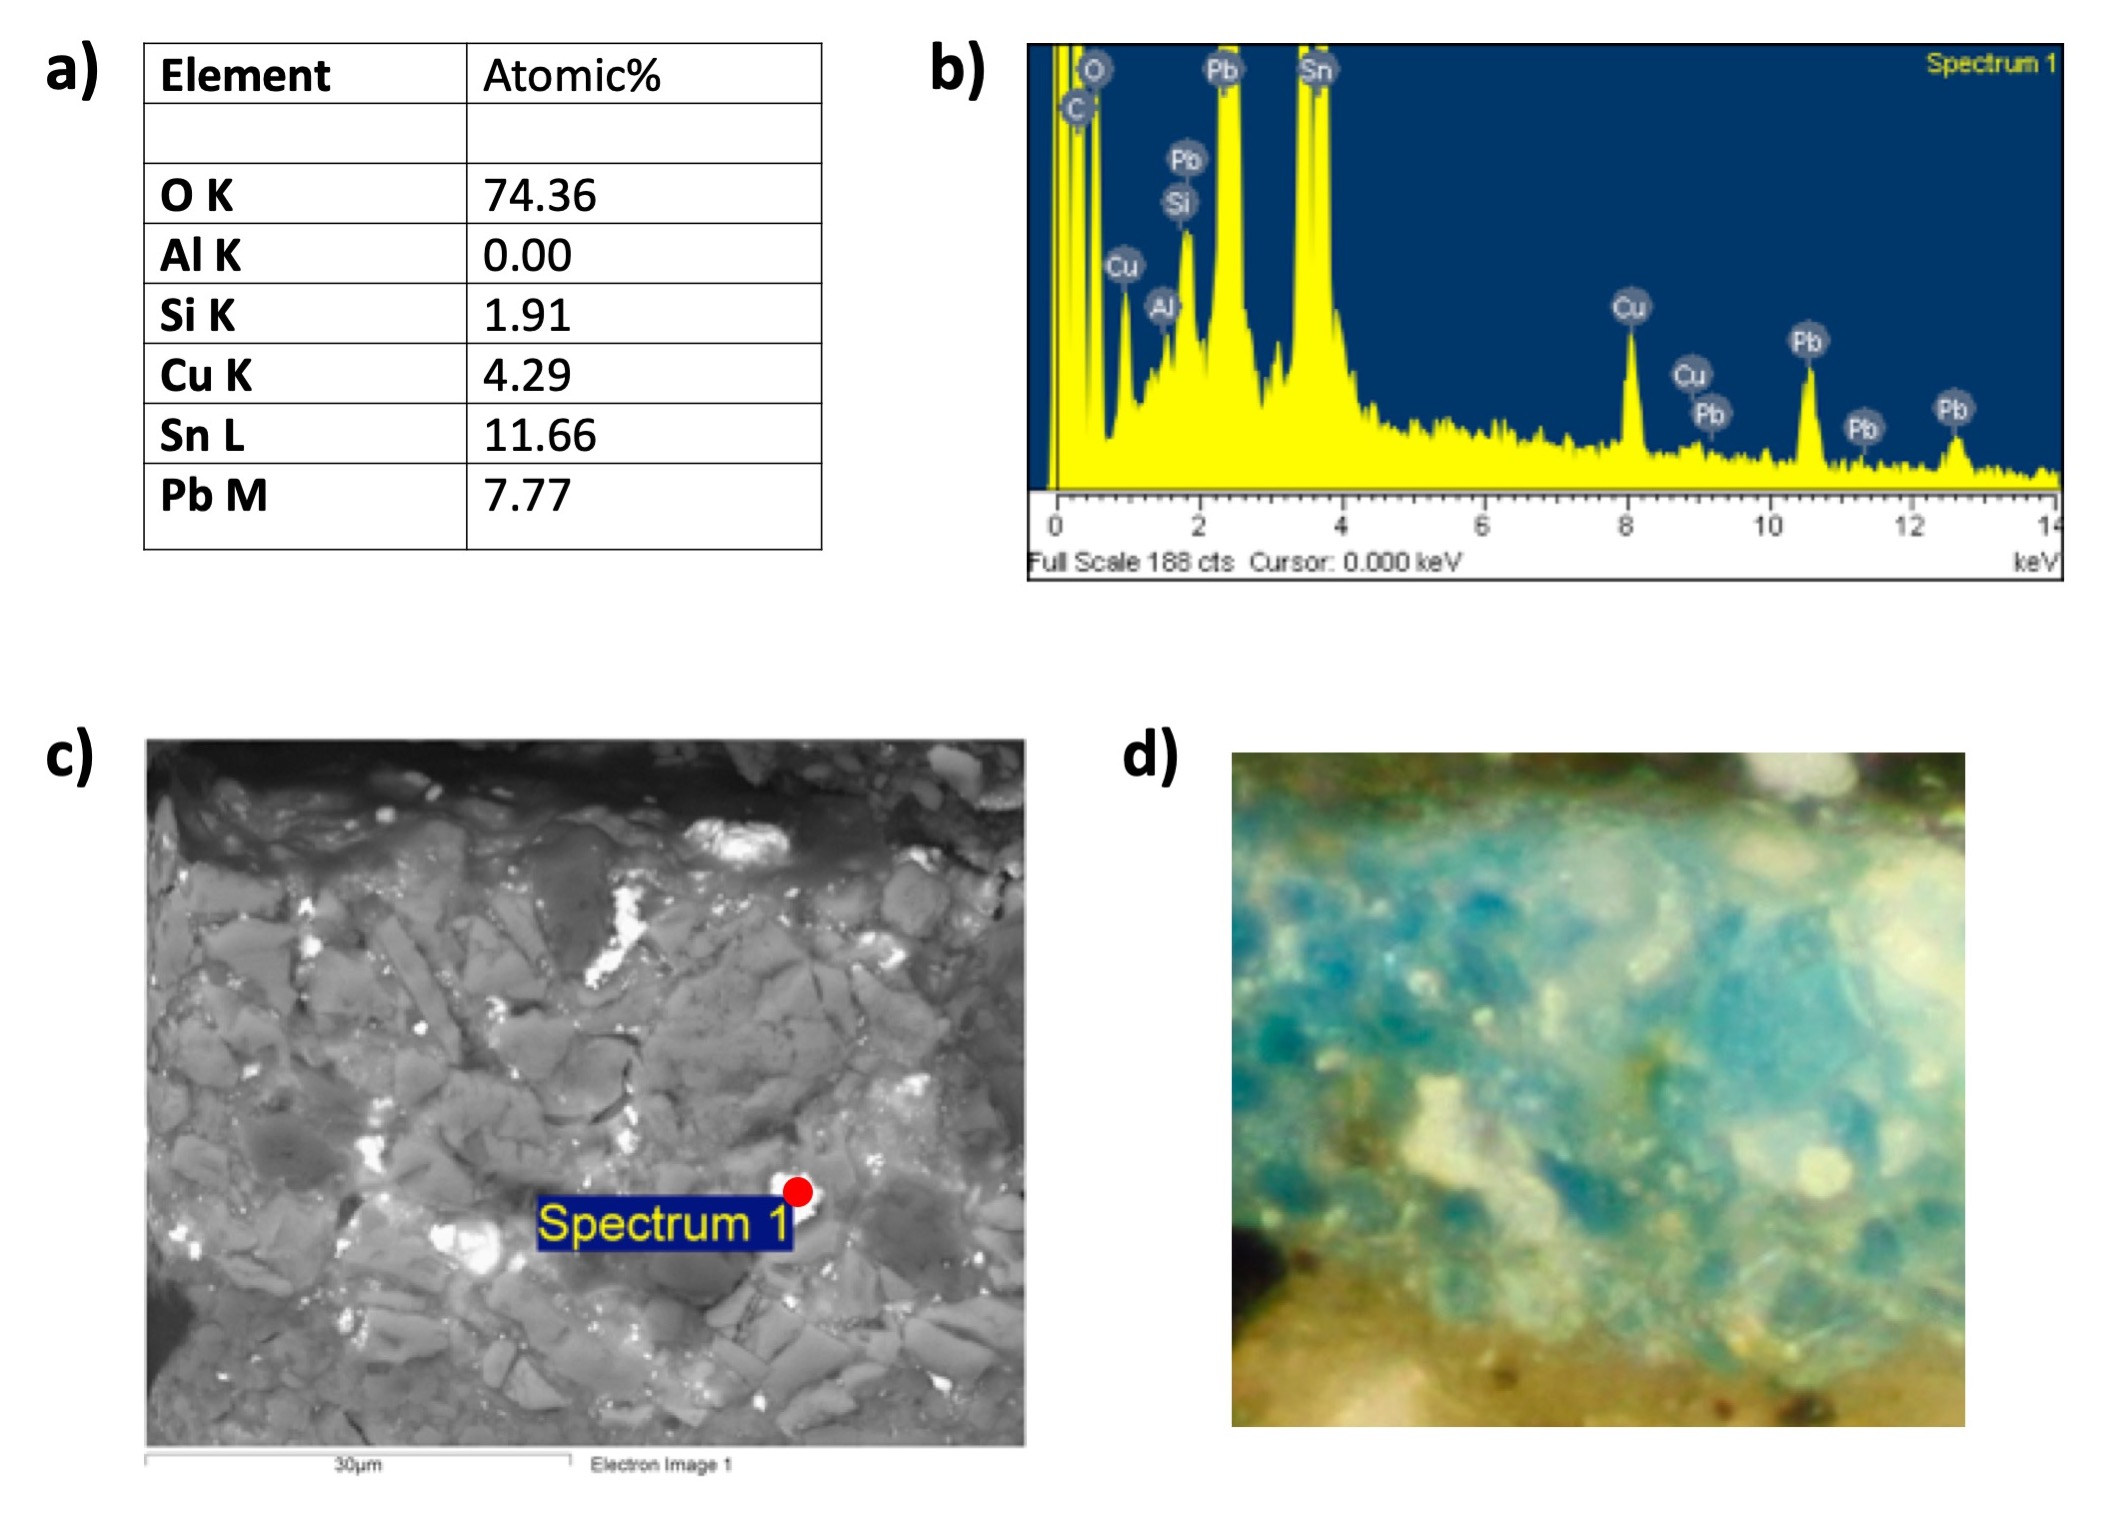
\includegraphics[width=\linewidth]{1259-28_pointspec}
\caption[EDS point spectrum data, sample 1259.28.]{EDS point spectrum data, sample 1259.28: \textbf{a)} Quantitative EDS results of particle showing lead and tin, \textbf{b)} EDS spectrum showing detection of lead and tin, \textbf{c)} SEM image showing point spectrum location, \textbf{d)} dark field microscope image showing point spectrum sample location, with no visually distinct particle present. Image is provided courtesy of Katharine Waldron, HKI.}
\label{fig:1259.28_pointspec}
\end{figure}

\begin{figure}[H]
\centering
\begin{minipage}[t]{\linewidth}
  \centering
  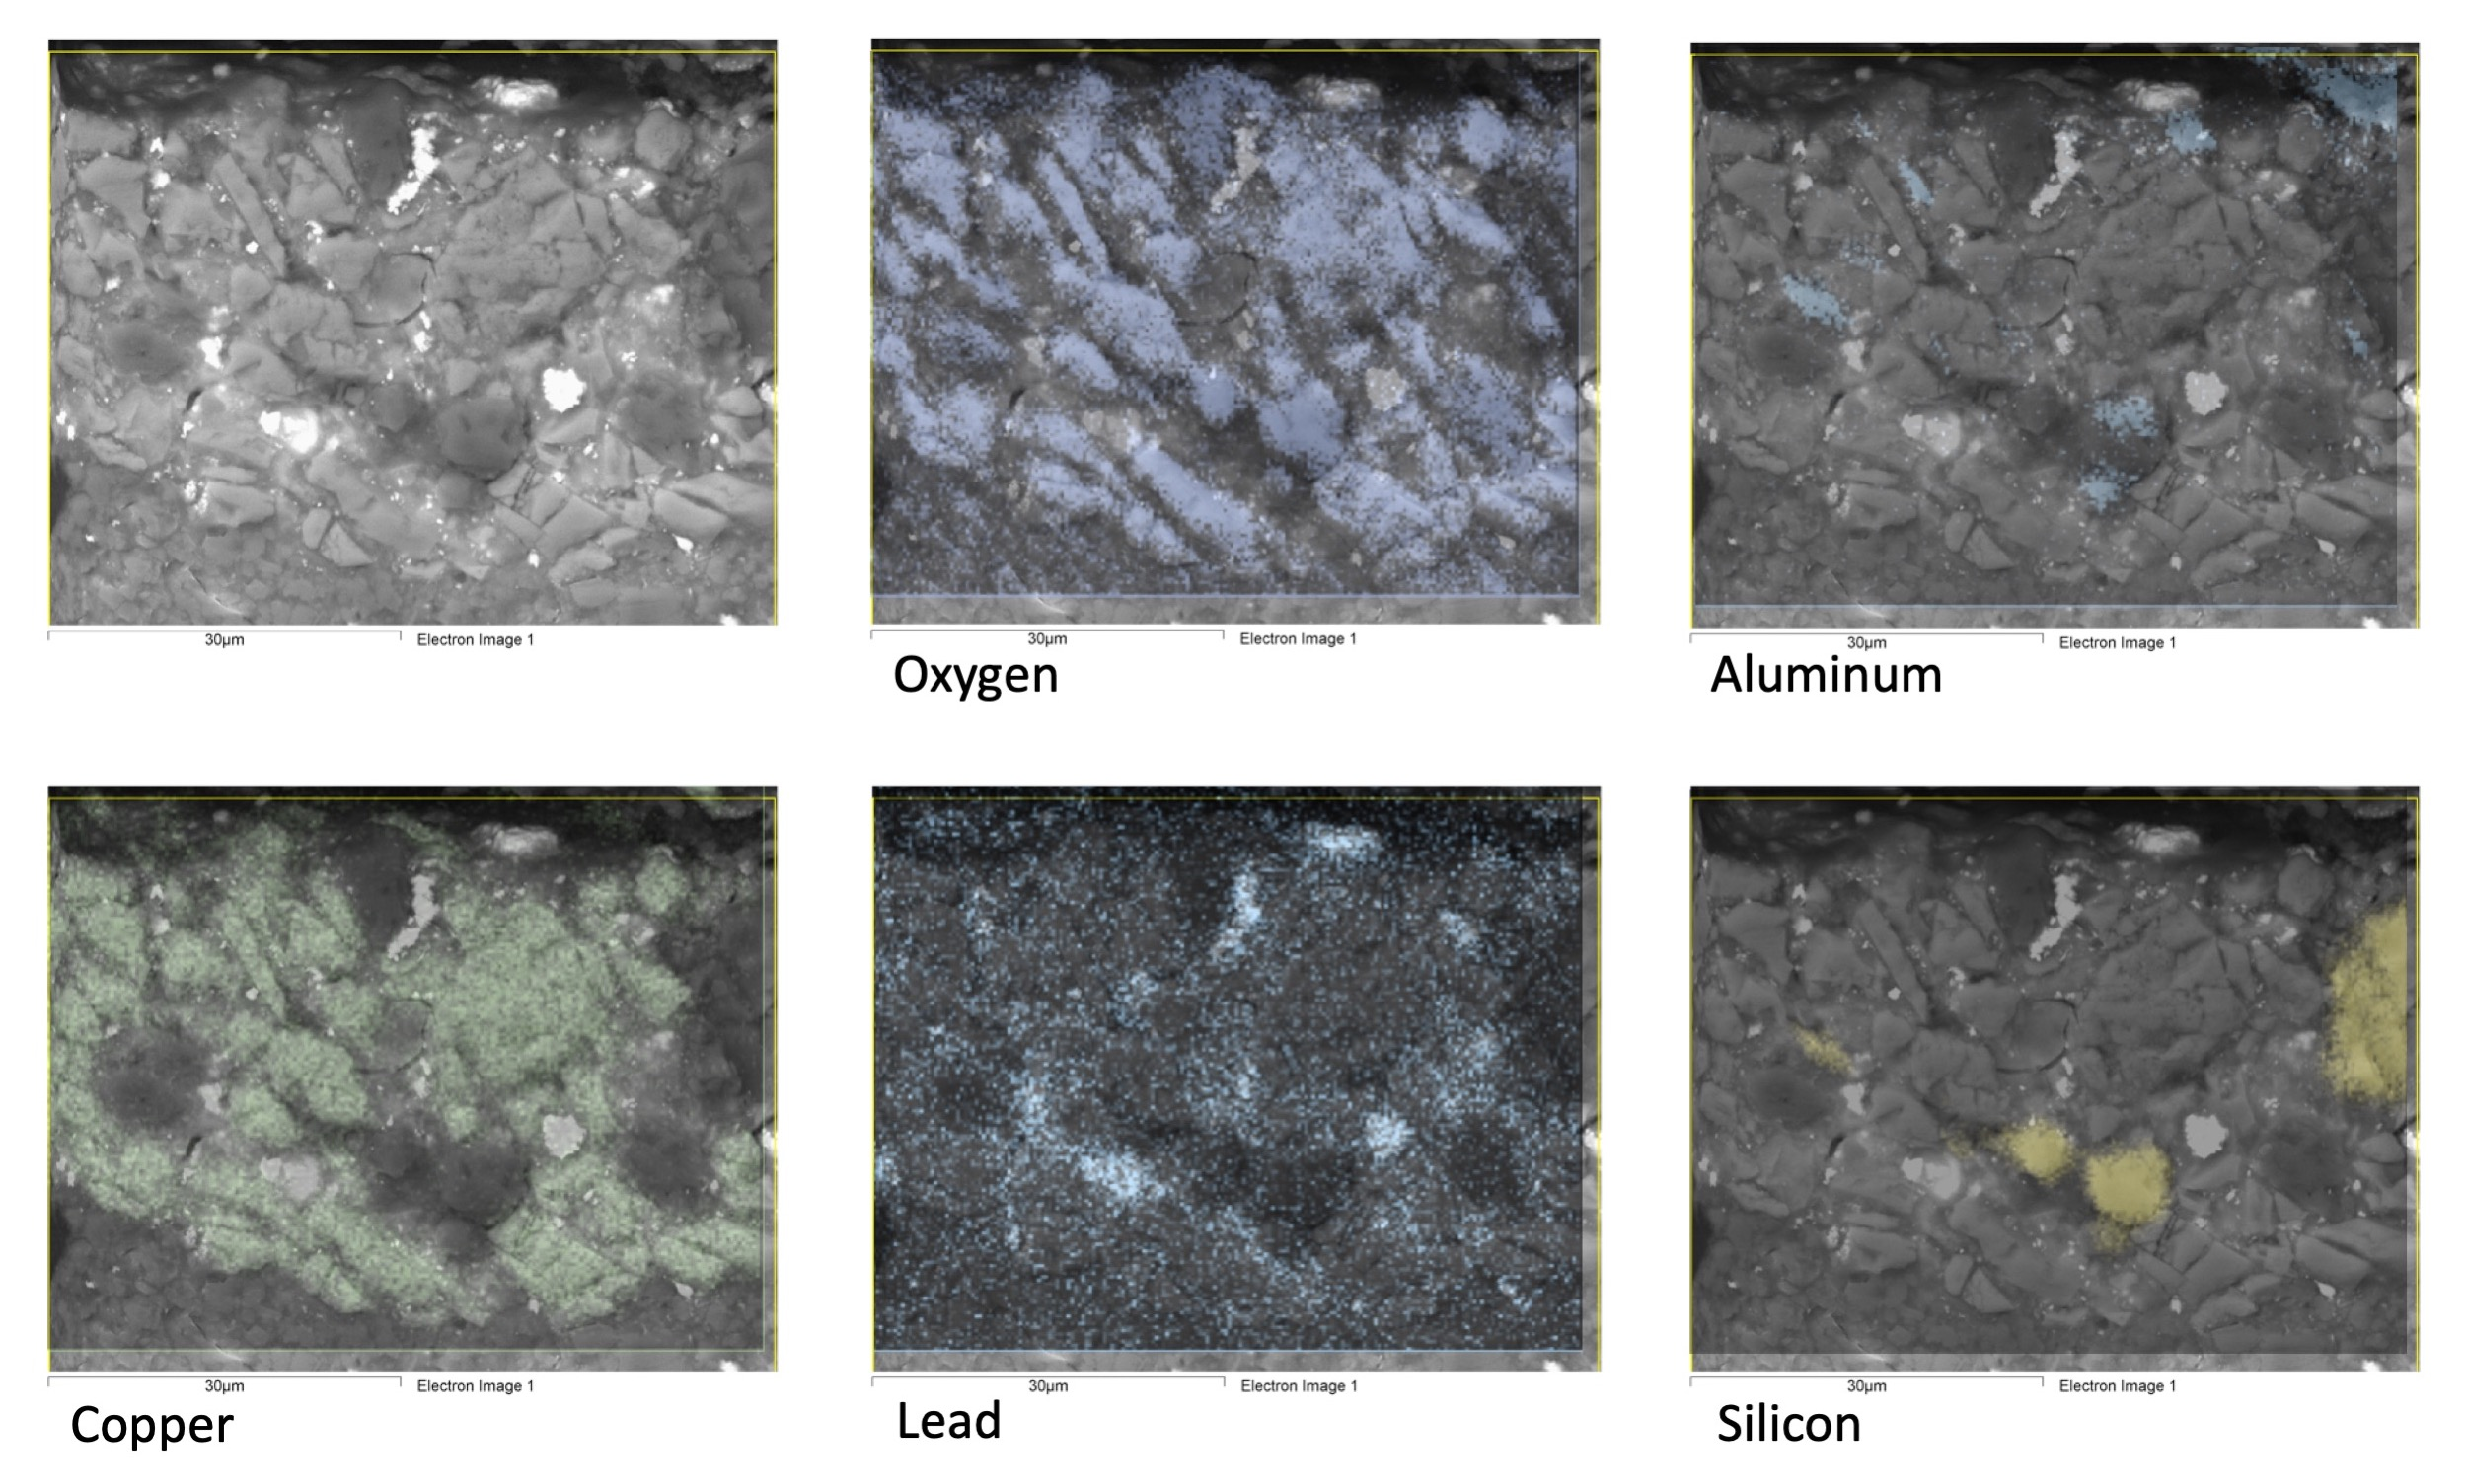
\includegraphics[width=0.9\linewidth]{1259-28_mapdata_1}
\hfill
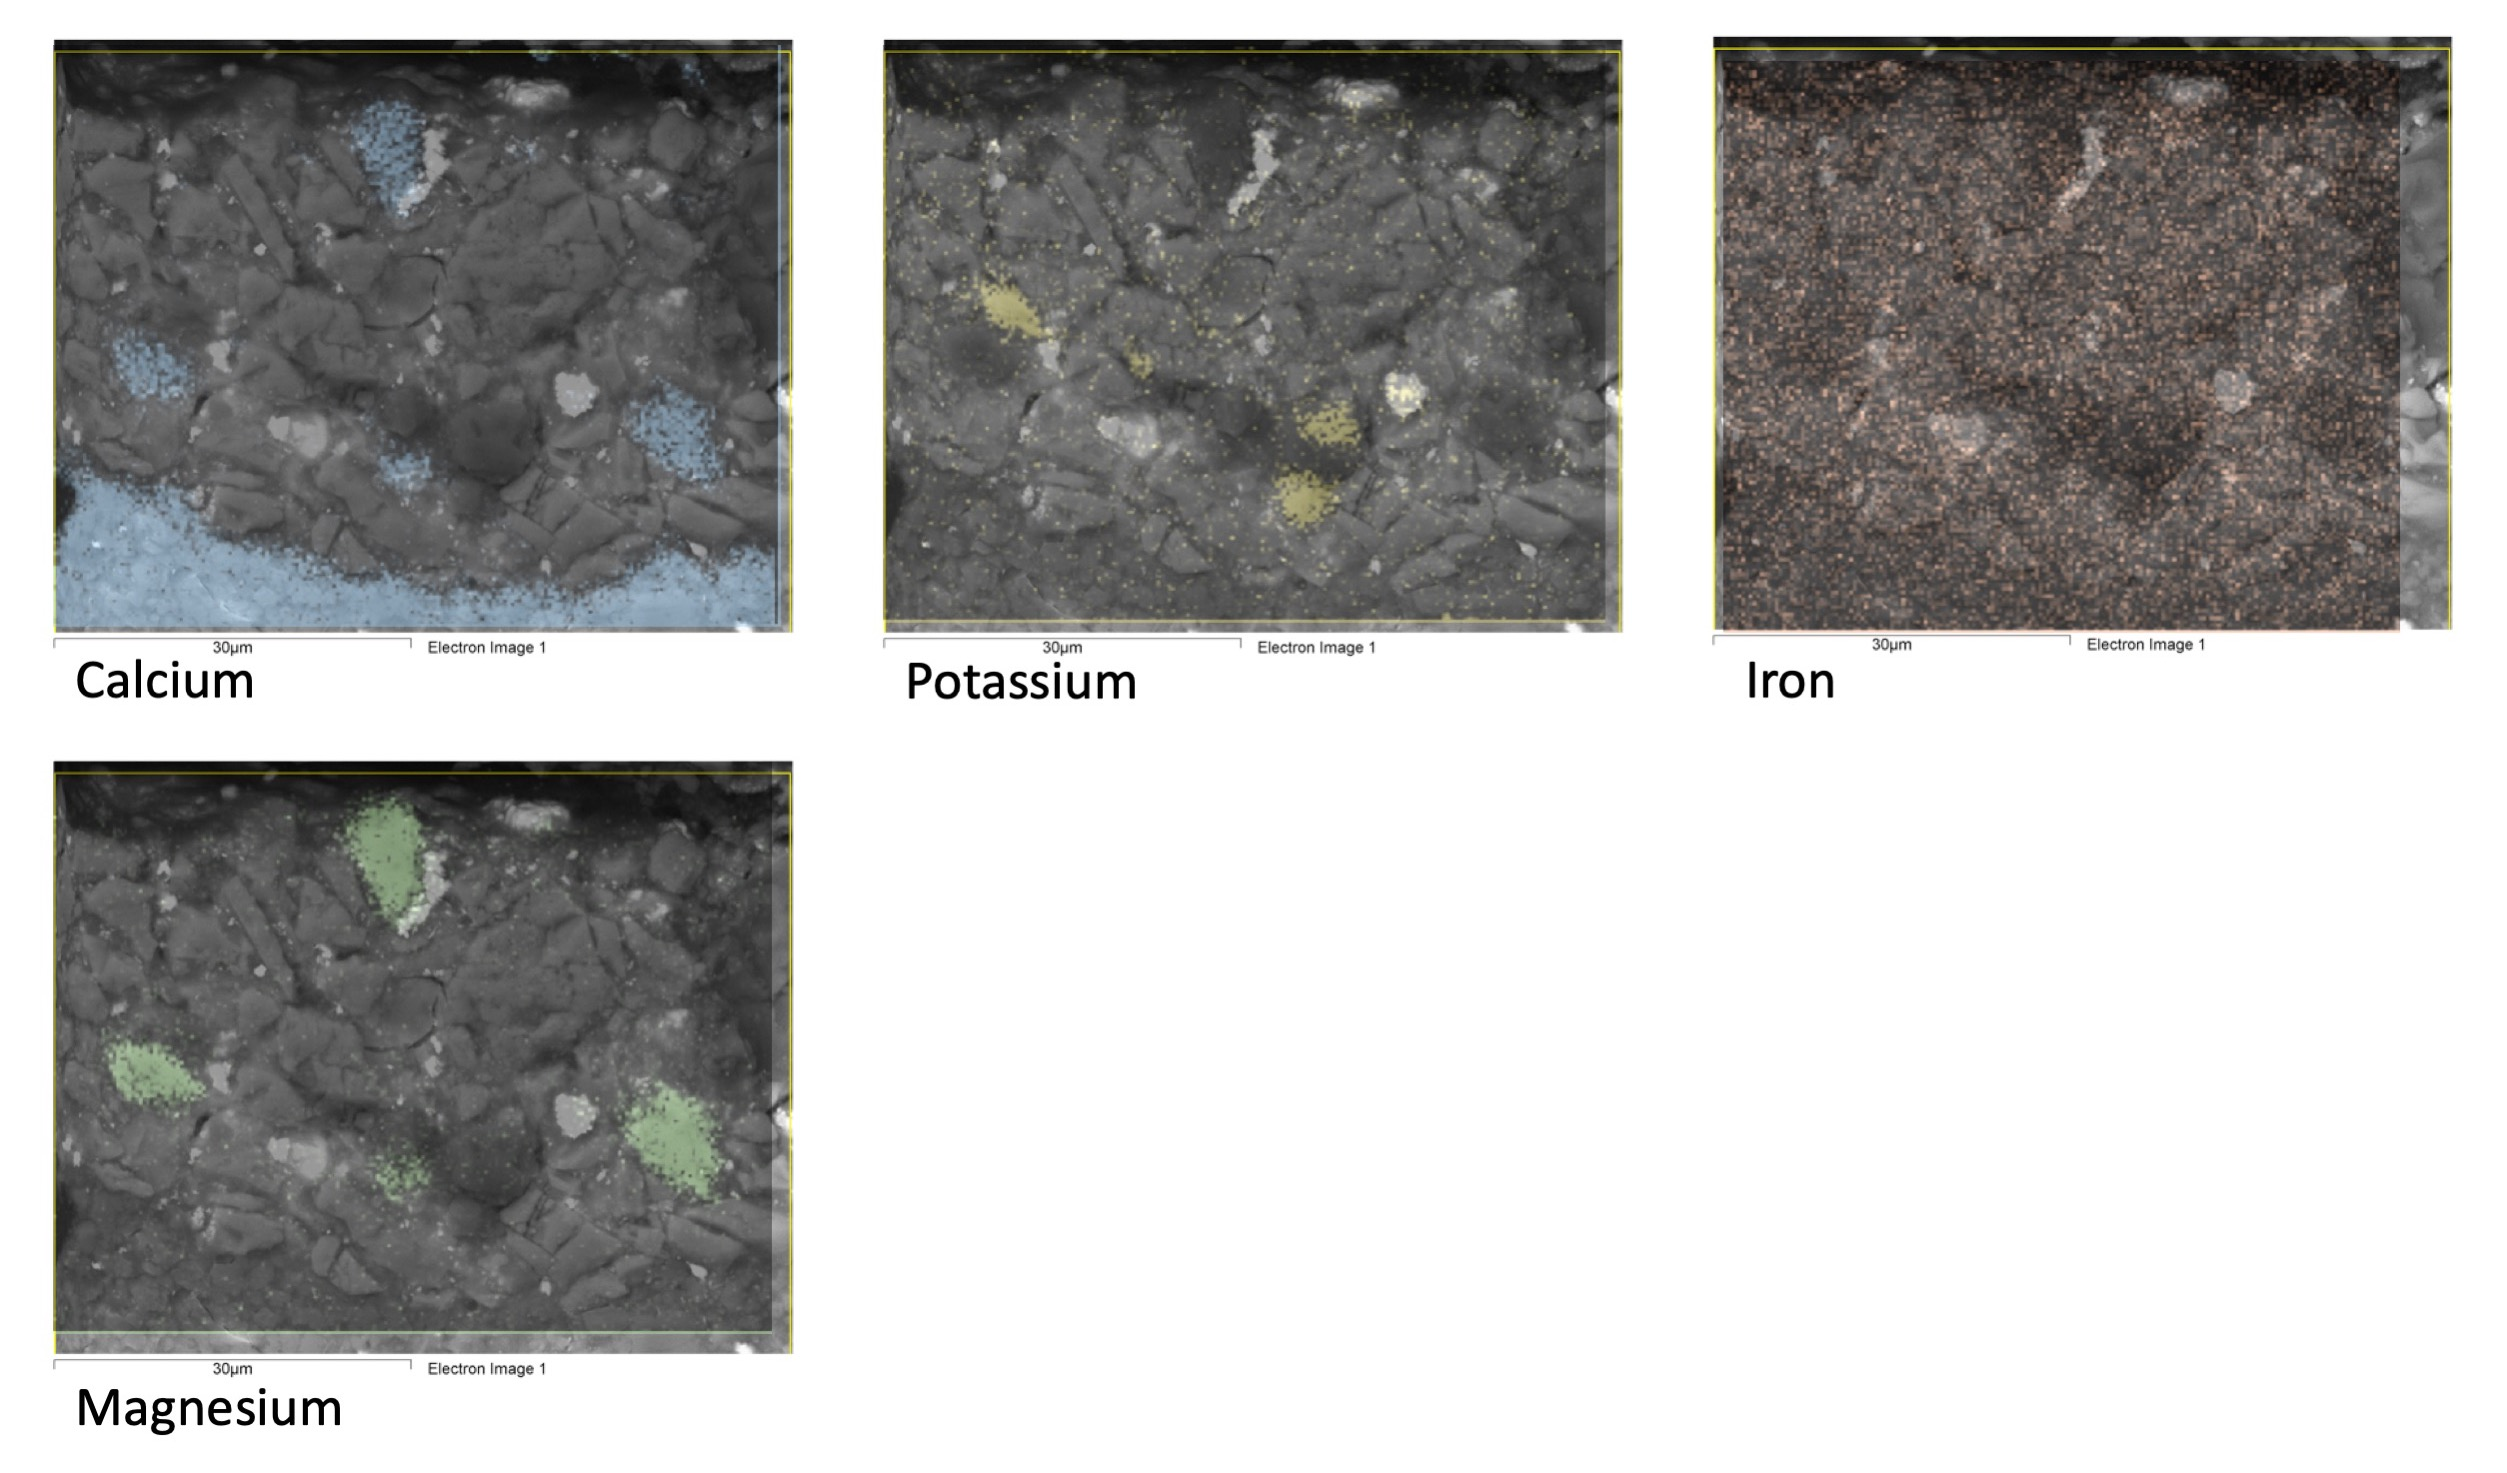
\includegraphics[width=0.9\linewidth]{1259-28_mapdata_2}
\hfill
\end{minipage}
\caption[EDS map data, sample 1259.28.]{EDS map data of sample 1259.28 showing locations of elements in an area of the azurite paint layer. Elements detected are O, Al, Cu, Pb, Si, Ca, K, Fe, Mg.}
\label{fig:1259.28_mapdata}
\end{figure}

\begin{figure}[H]
\centering
  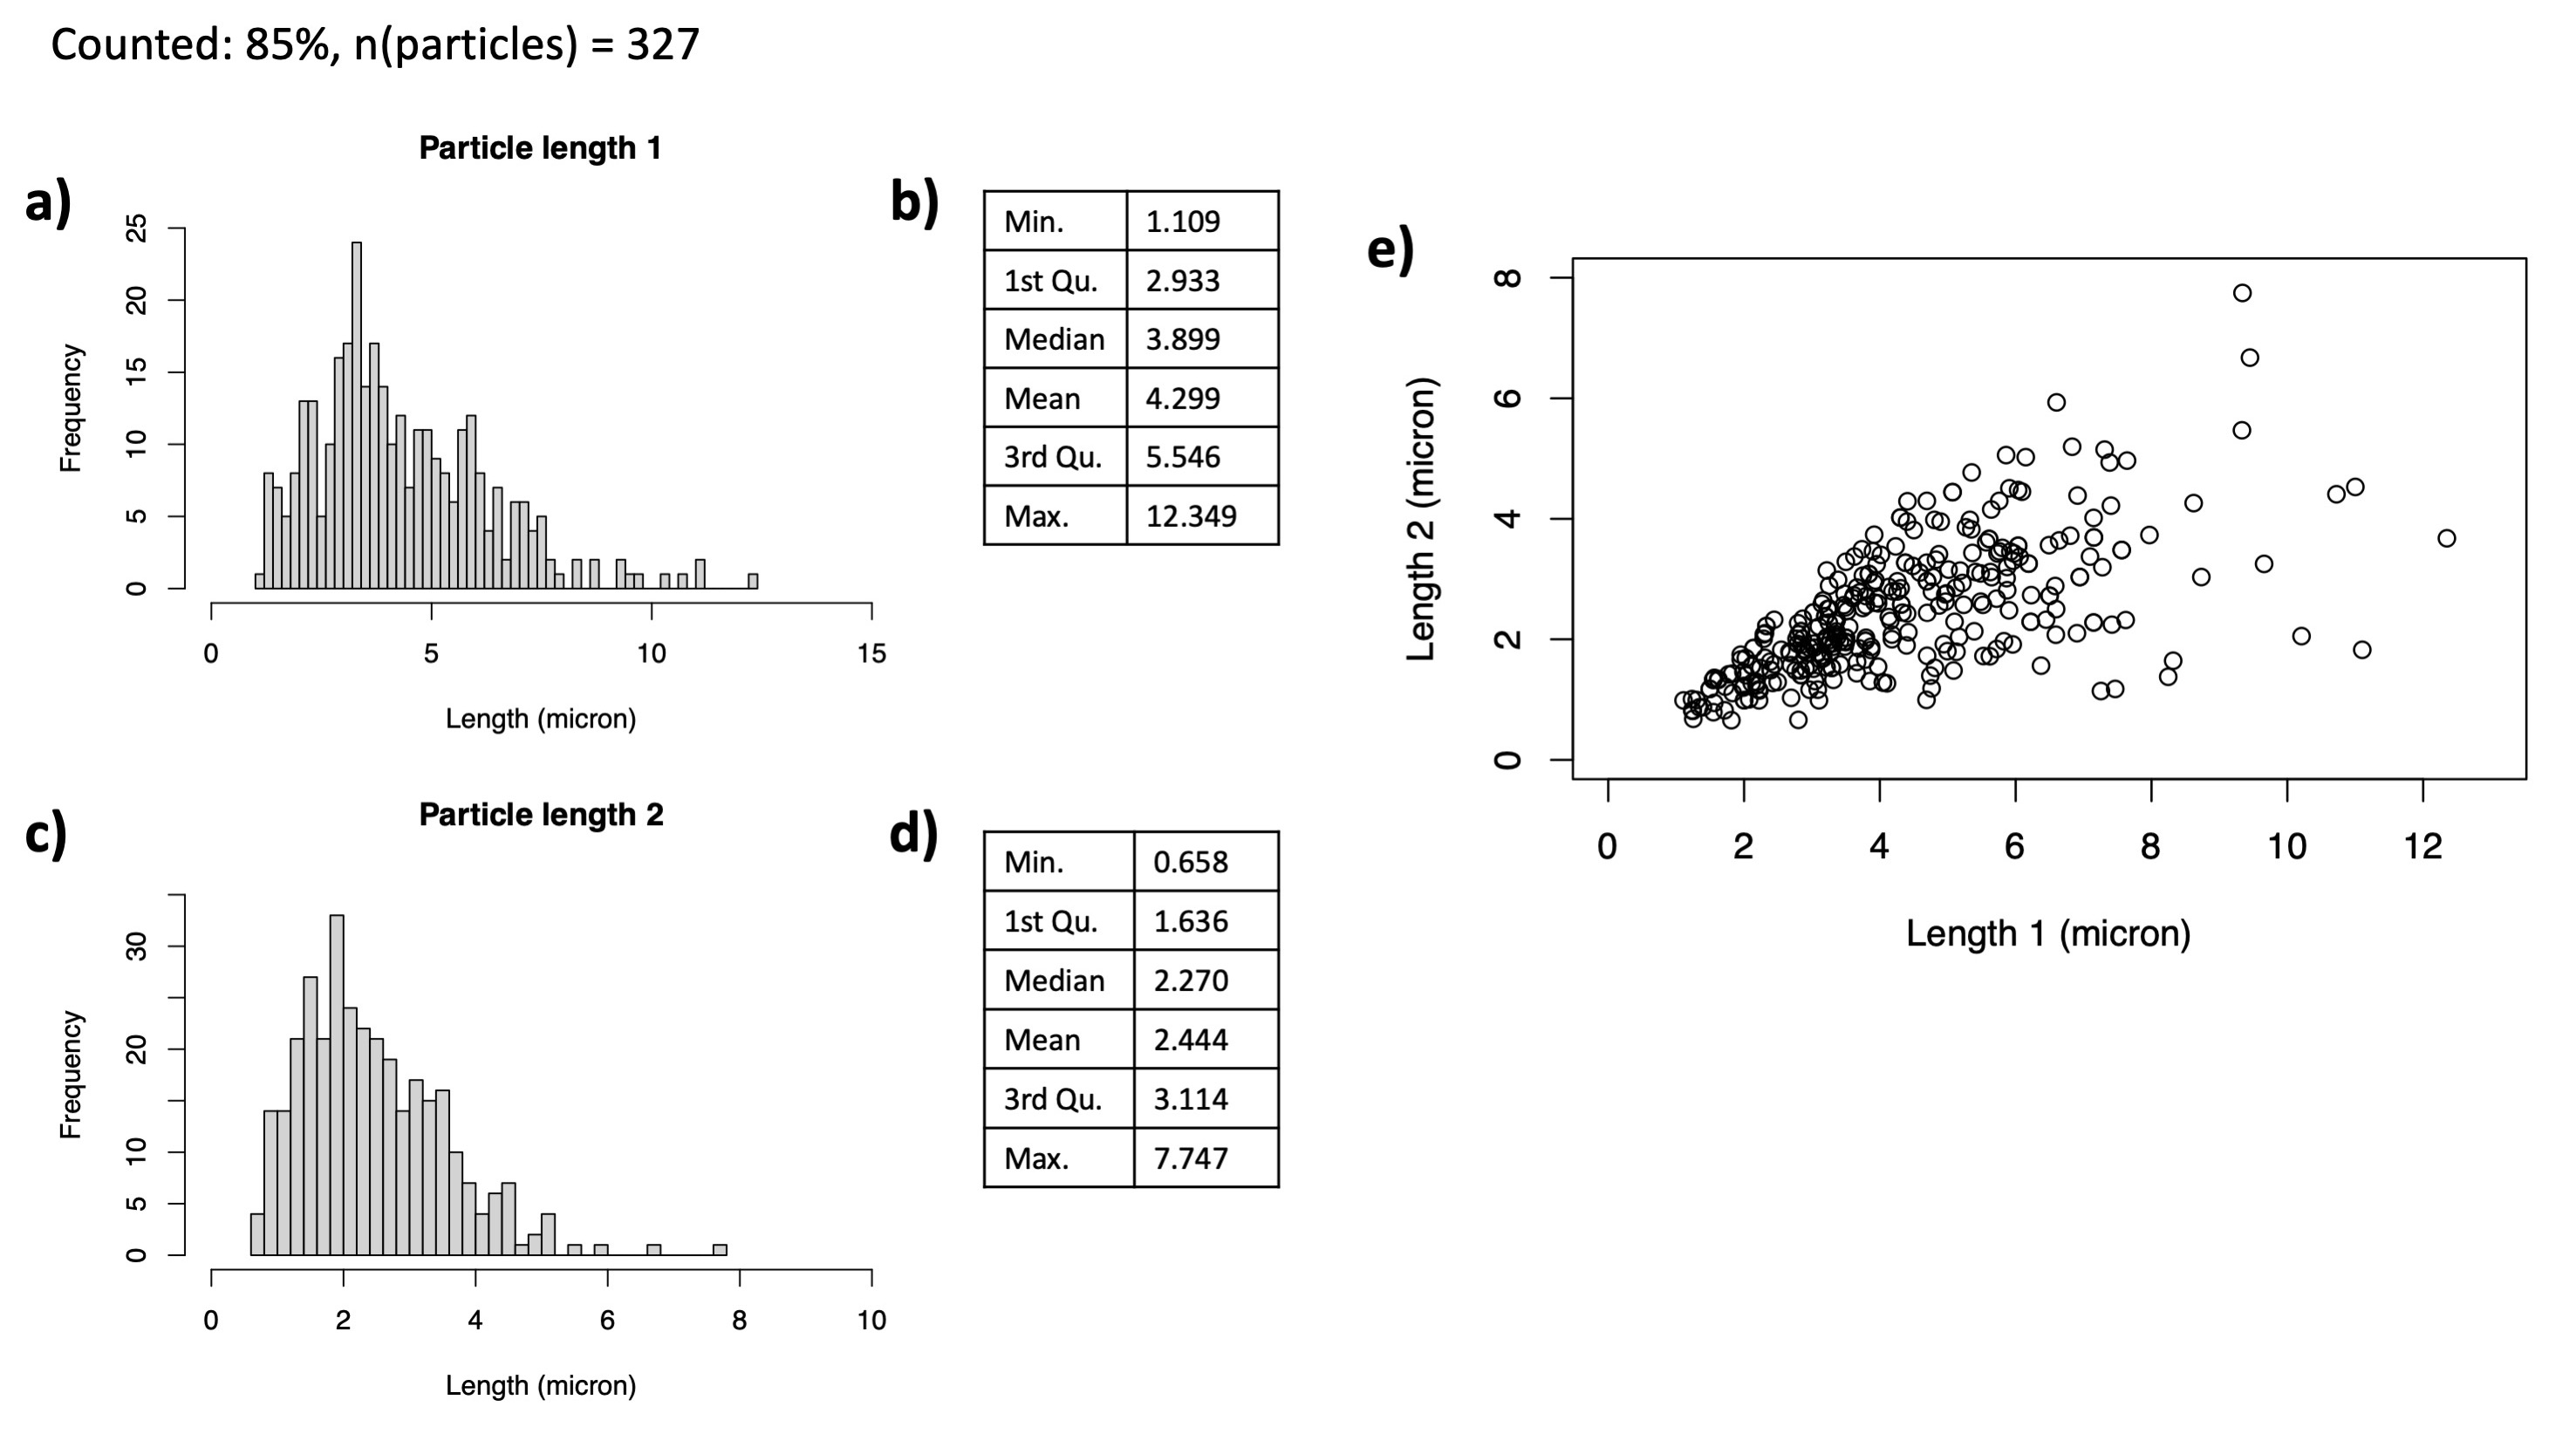
\includegraphics[width=\linewidth]{1259-28_partsize}
\caption[Particle size distribution, sample 1259.28.]{Particle size distribution of sample 1259.28: \textbf{a)} Histogram showing distribution of particle length 1 values. \textbf{b)} Descriptive statistics for particle length 1 data. \textbf{c)} Histogram showing distribution of particle length 2 values. \textbf{d)} Descriptive statistics for particle length 2 data. \textbf{e)} Graph of length 1 versus length 2 showing the degree of skew.}
\label{fig:1259.28_partsize}
\end{figure}


\section{Sample 1259.29}

\textit{Figures \ref{fig:1259.29_imgs}}-\textit{\ref{fig:1259.29_partsize}} show SEM/dark field images, EDS map data, and particle size data for 1259.29. SEM images show densely packed azurite particles with some lower atomic weight particles interspersed. The dark field image shows primarily yellow and white impurities. The large blob shapes in the SEM images are resin bubbles from the embedding process.

Map data confirms azurite, rutile, iron oxide, dolomite, calcium phosphate (possibly apatite), . Lead and zinc maps do not show localisation, suggesting these elements are not present in significant levels. There is also a mineral containing primarily potassium present. Particle size data shows a small number of outlying large particles and primarily small, skewed particles clustered around 4.5 x 2.5 $\mu$m. Overall this indicates fine and consistent grinding preparation. 

\begin{figure}[H]
  \centering
  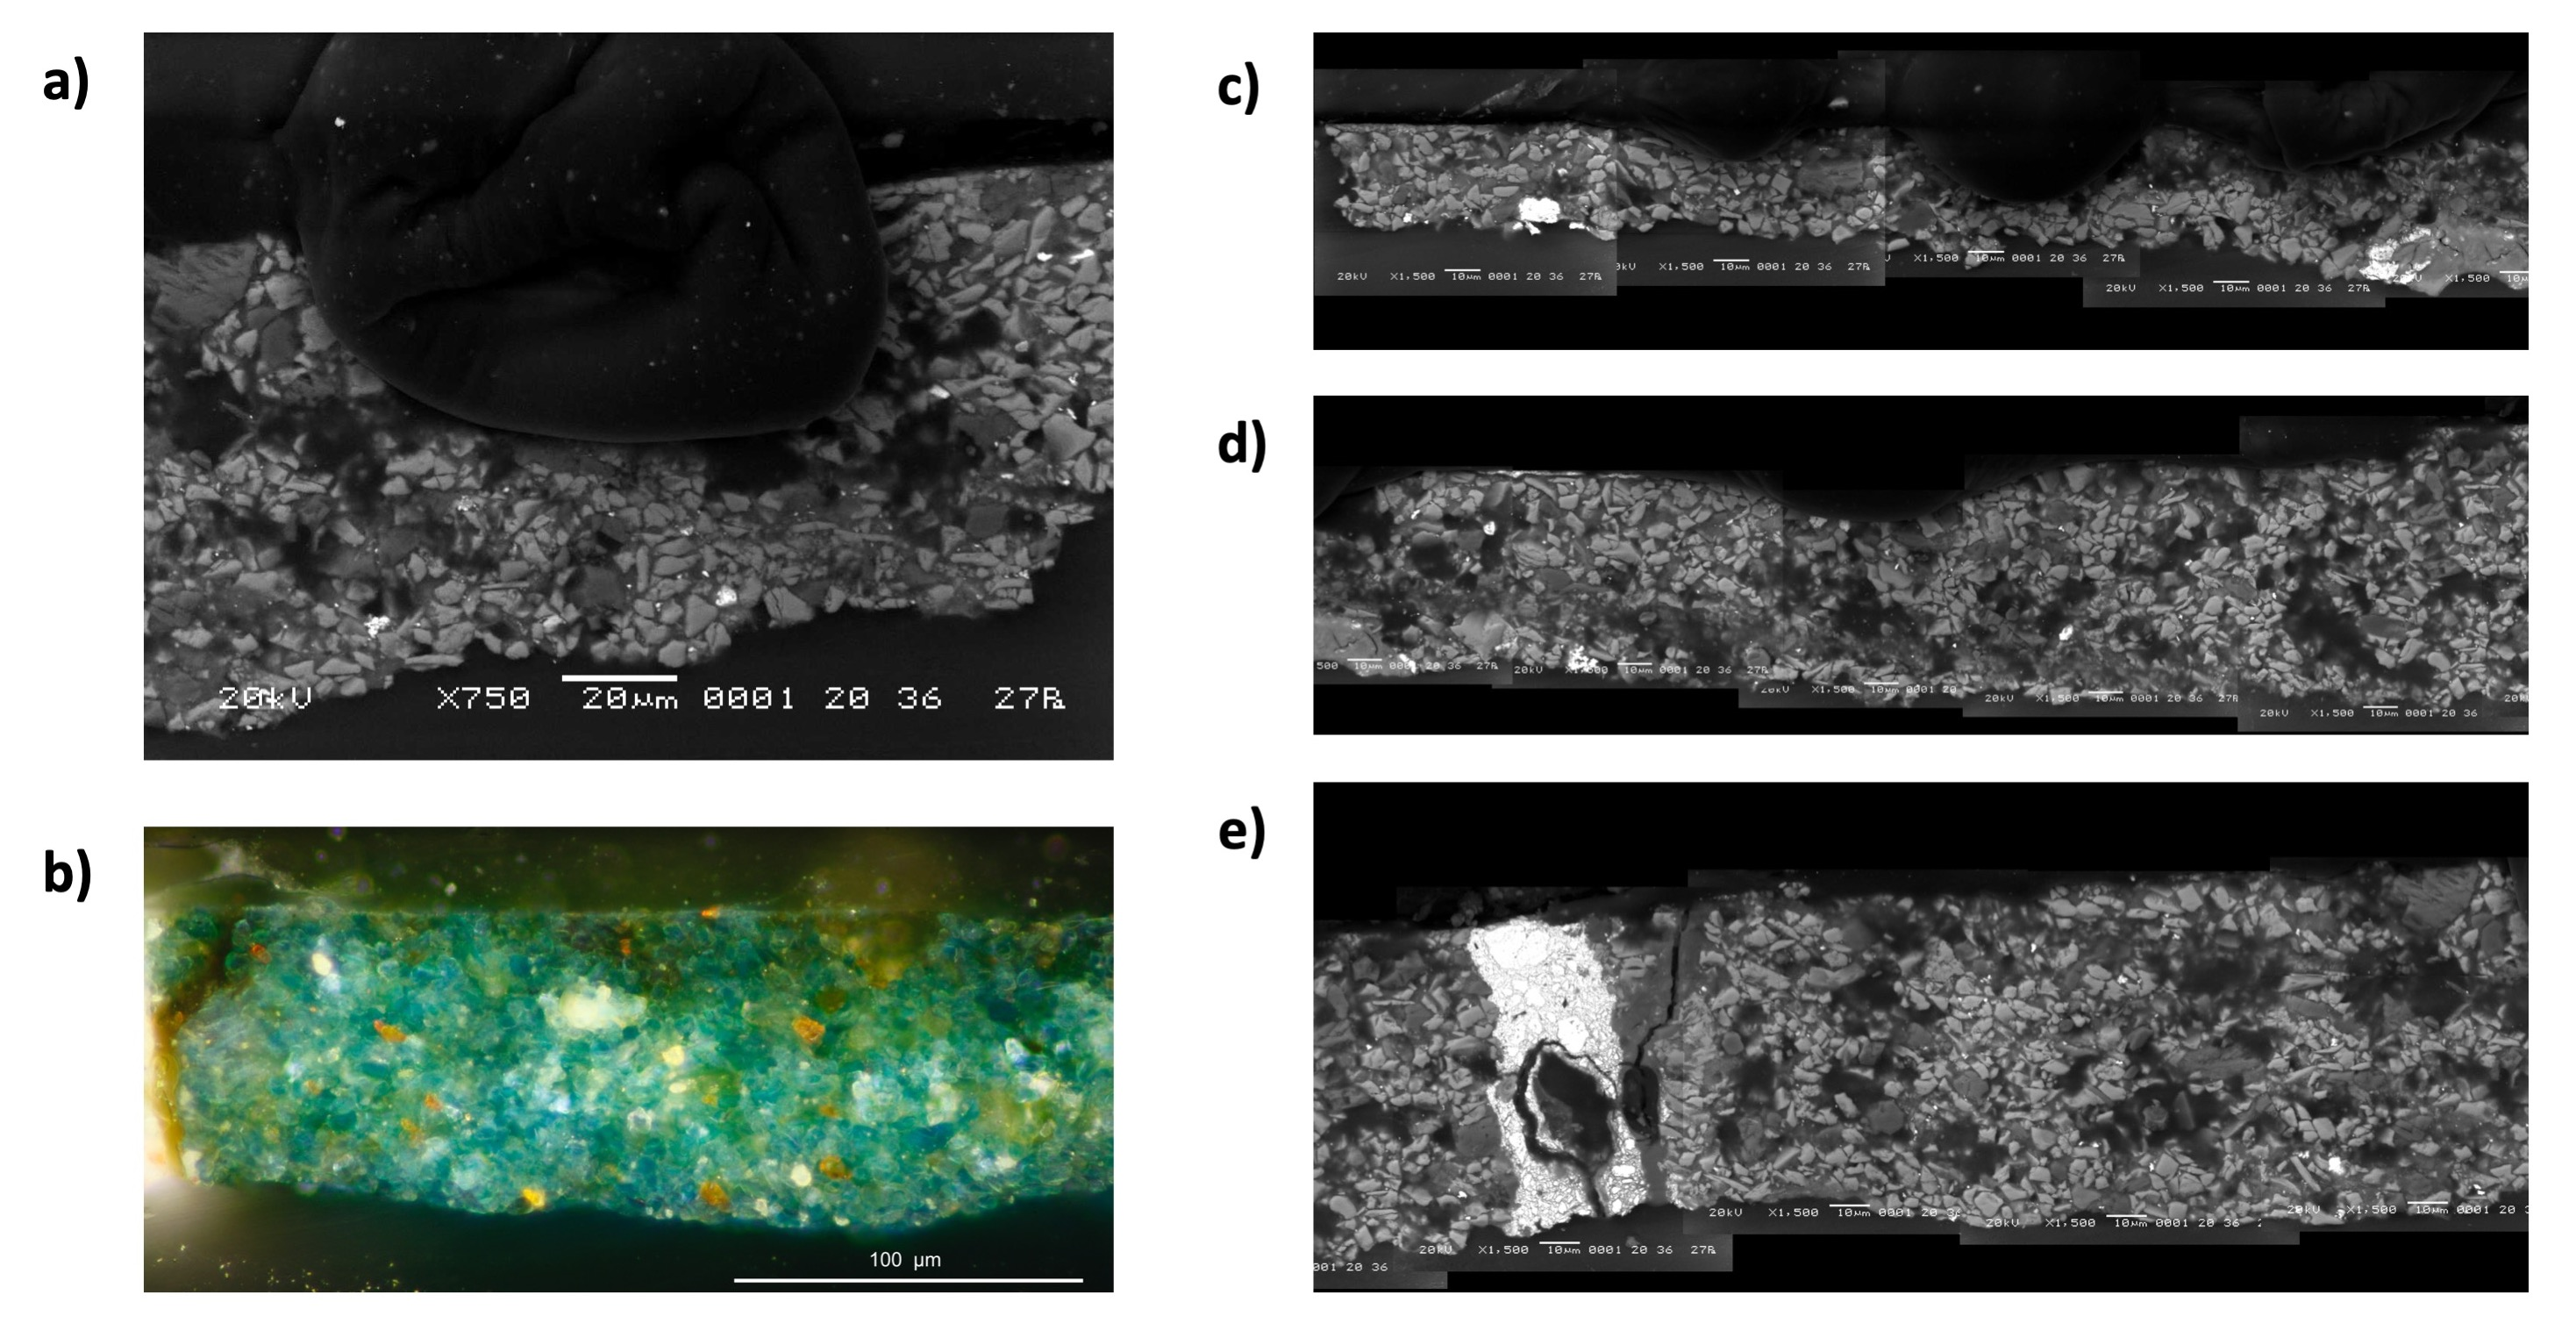
\includegraphics[width=\linewidth]{1259-29_imgs}
\caption[SEM and dark field images of sample 1259.29.]{SEM and dark field images of sample 1259.29: \textbf{a)} 750x magnification, \textbf{b)} dark field microscope image of sample, \textbf{c-e)} 1500x magnification composite image of entire sample region. The dark blobs on sample surface in SEM images are resin patches (and are transparent in dark field images). Dark field microscope images courtesy of Katharine Waldron, HKI.}
\label{fig:1259.29_imgs}
\end{figure}

\begin{figure}[H]
\centering
\begin{minipage}[t]{\linewidth}
  \centering
  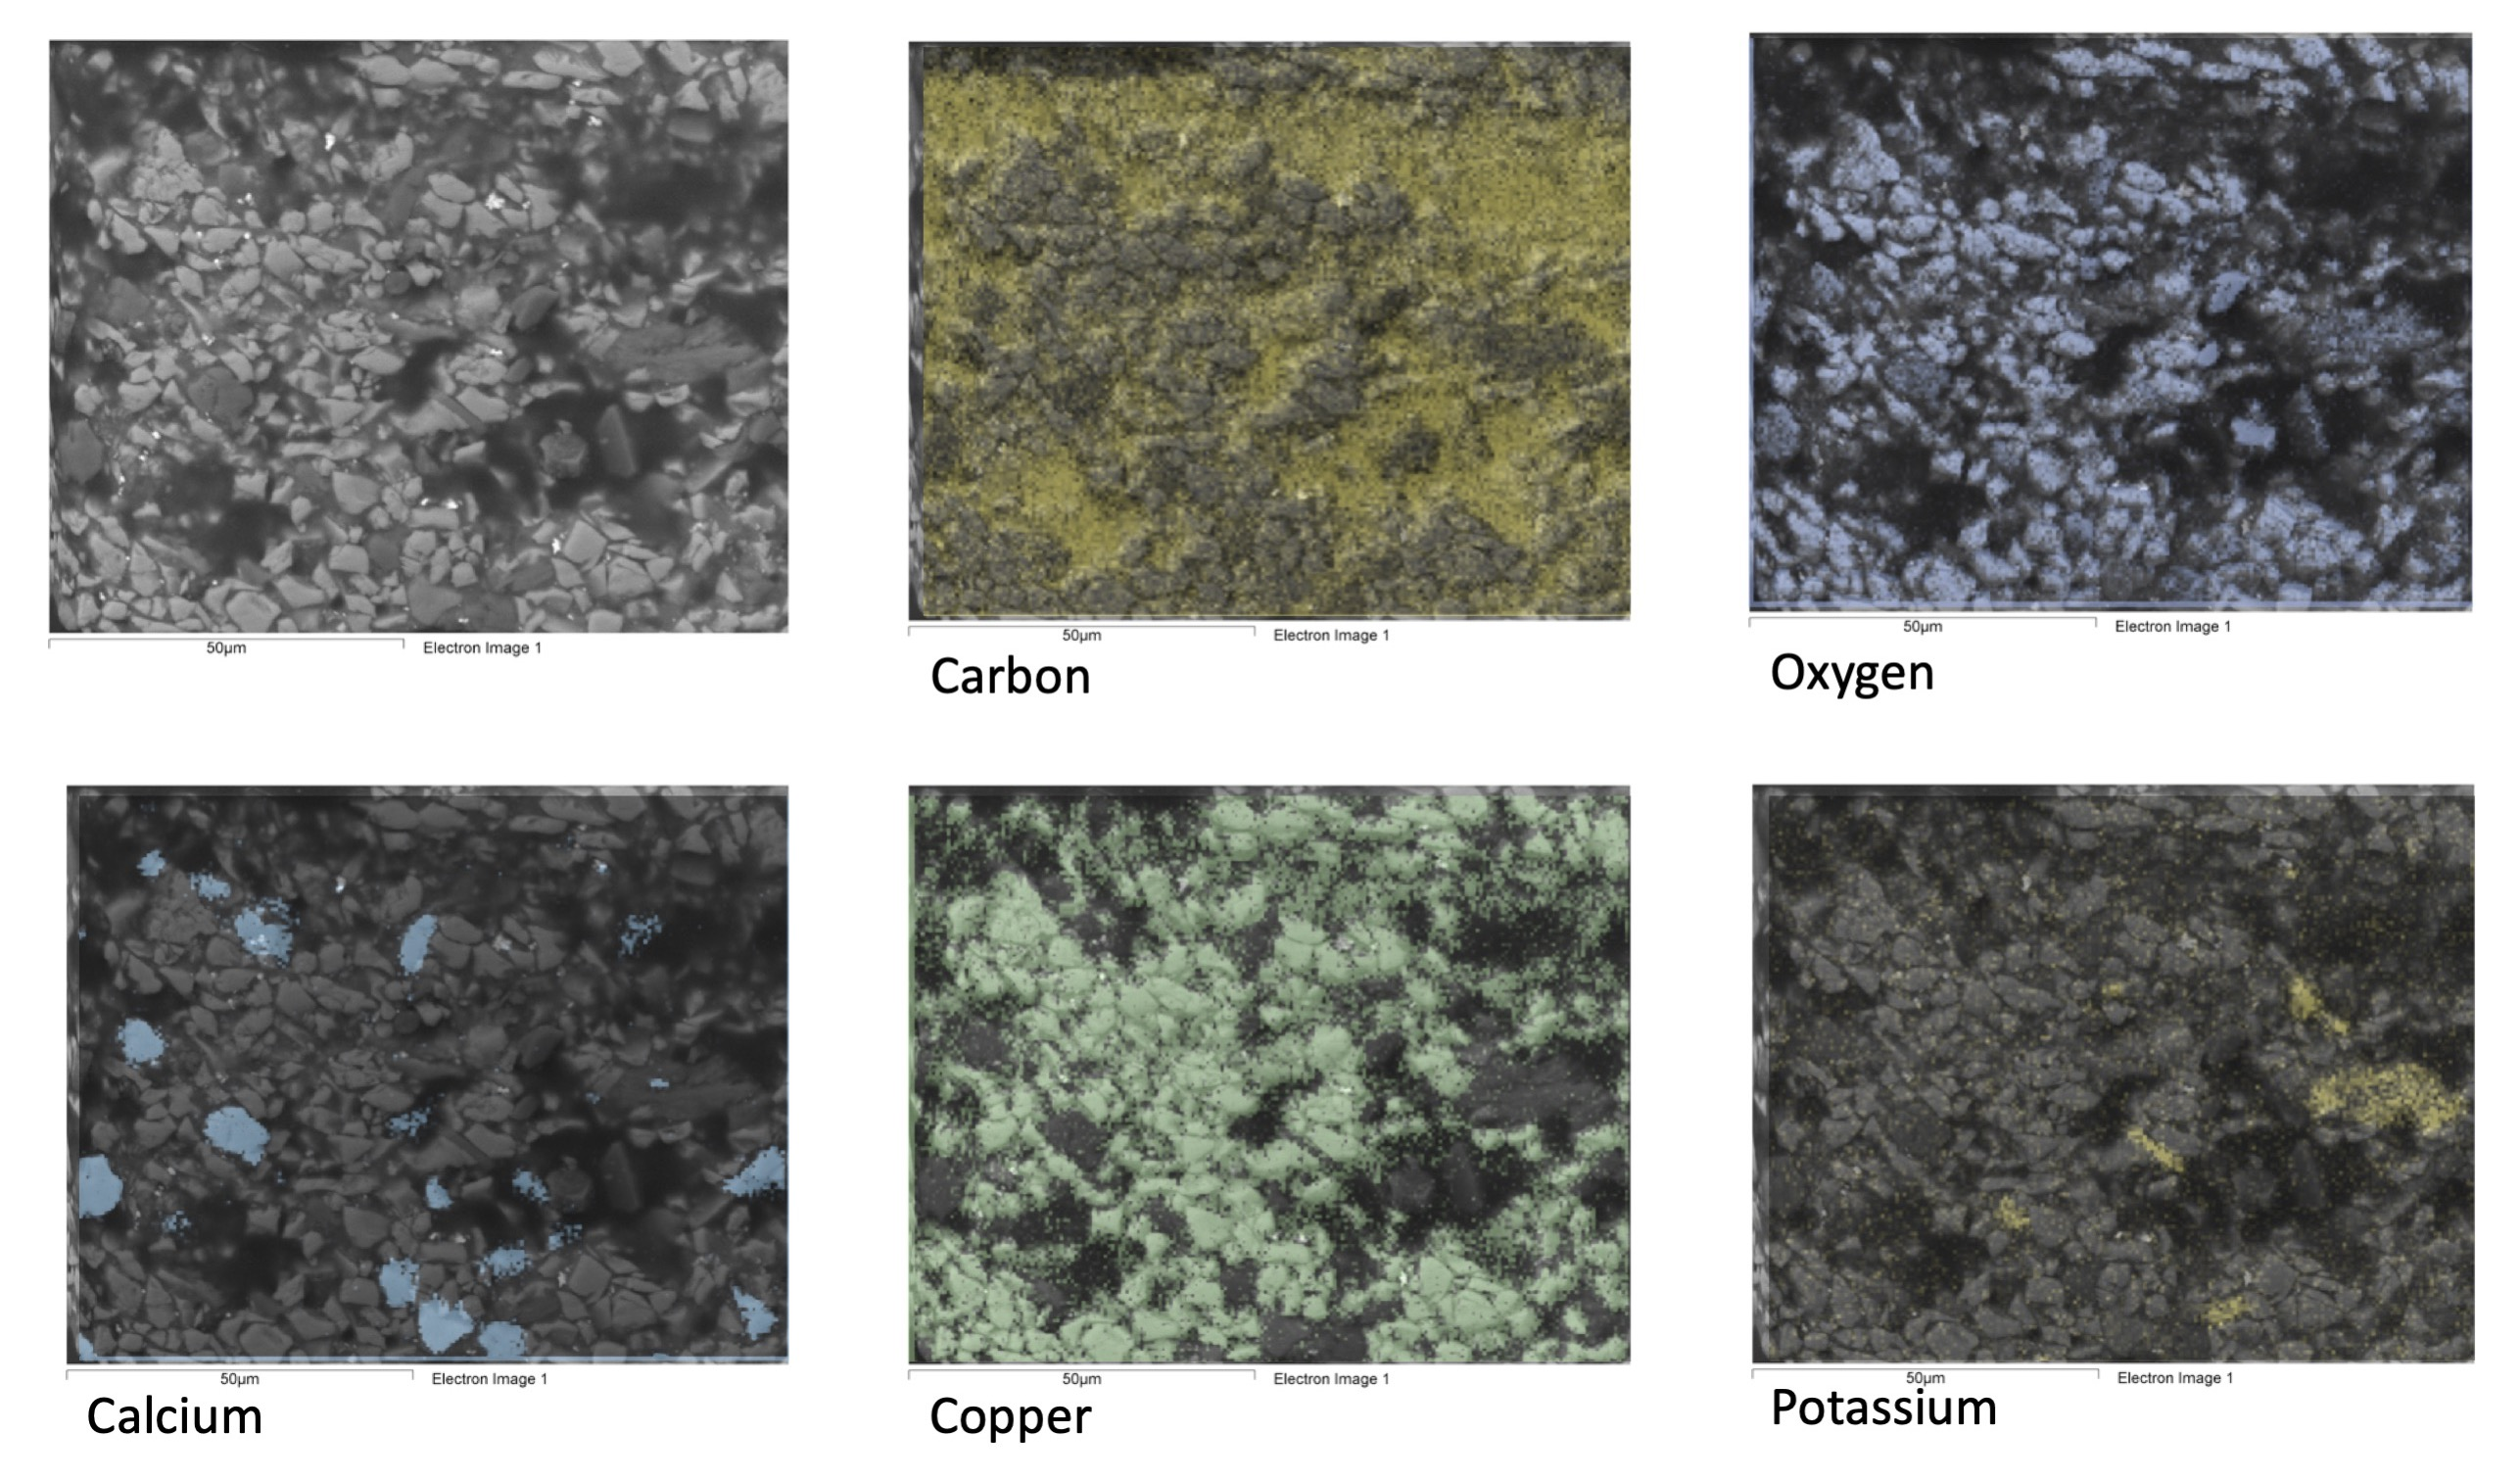
\includegraphics[width=0.9\linewidth]{1259-29_mapdata_1}
\hfill
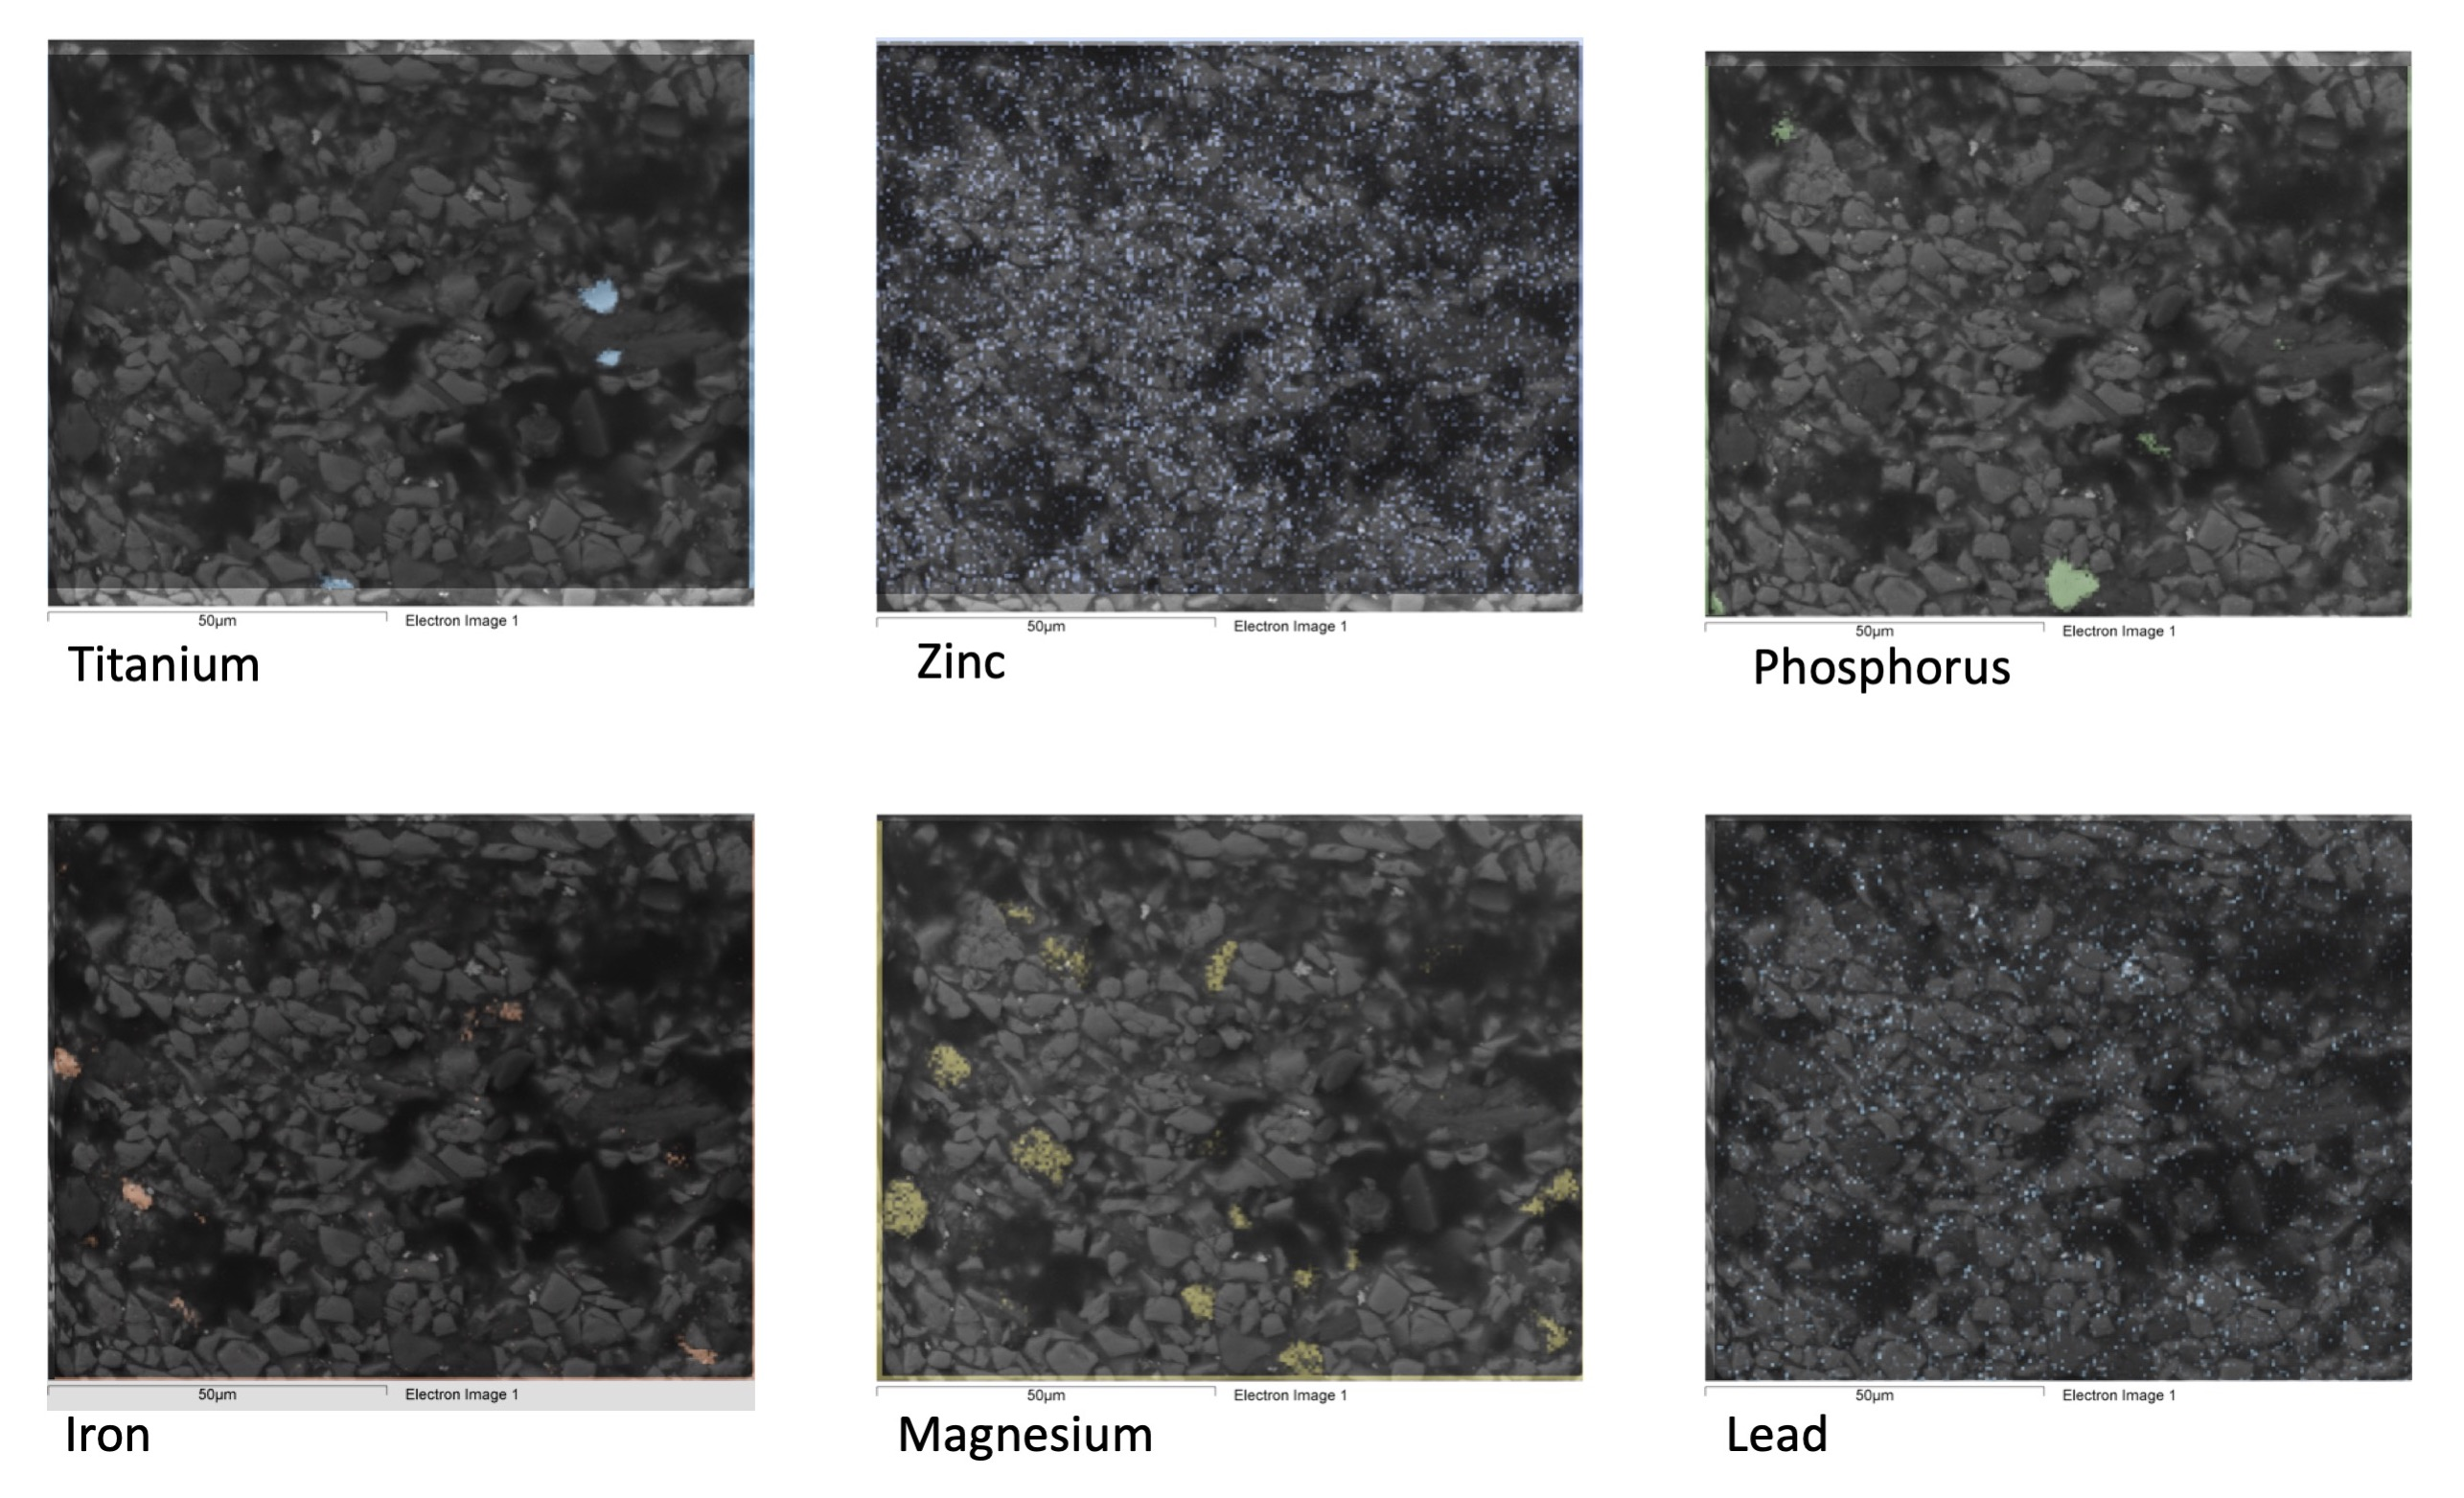
\includegraphics[width=0.9\linewidth]{1259-29_mapdata_2}
\hfill
\end{minipage}
\caption[EDS map data, sample 1259.29.]{EDS map data of sample 1259.29 showing locations of elements in an area of the azurite paint layer. Elements detected are C, O, Ca, Cu, K, Ti, Zn, P, Fe, Mg, and Pb.}
\label{fig:1259.29_mapdata}
\end{figure}


\begin{figure}[H]
\centering
  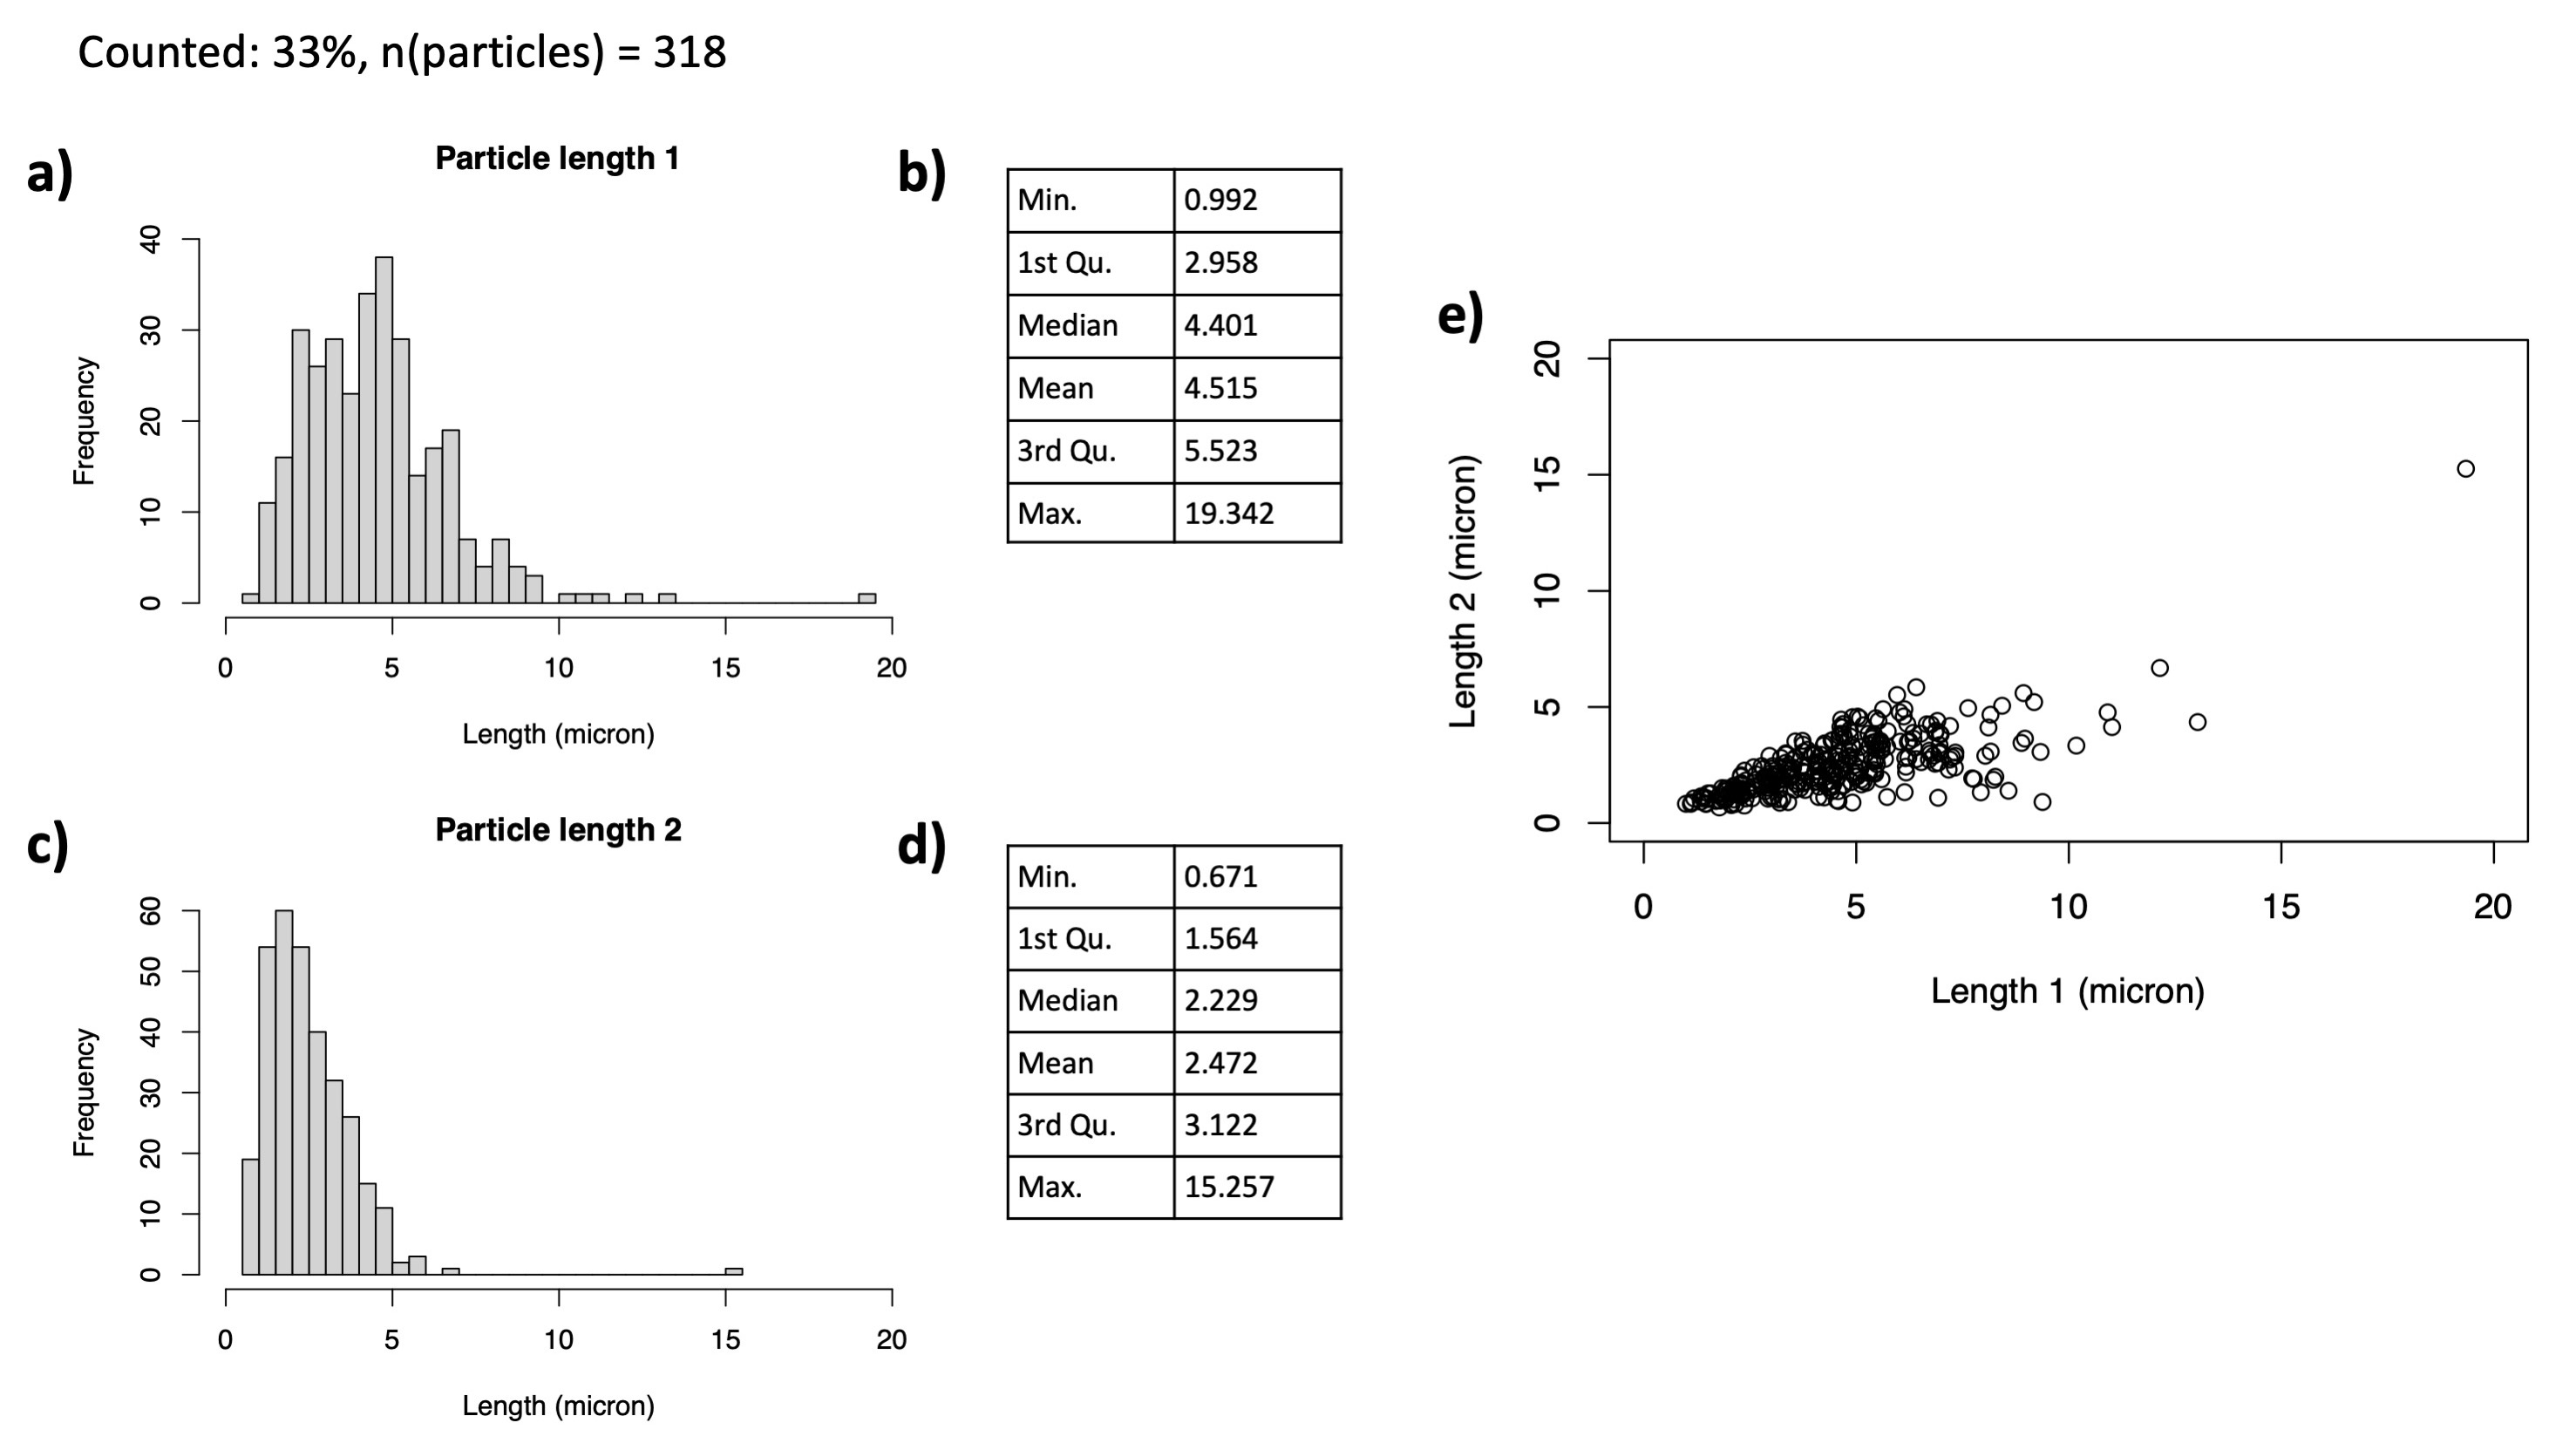
\includegraphics[width=\linewidth]{1259-29_partsize}
\caption[Particle size distribution, sample 1259.29.]{Particle size distribution of sample 1259.29: \textbf{a)} Histogram showing distribution of particle length 1 values. \textbf{b)} Descriptive statistics for particle length 1 data. \textbf{c)} Histogram showing distribution of particle length 2 values. \textbf{d)} Descriptive statistics for particle length 2 data. \textbf{e)} Graph of length 1 versus length 2 showing the degree of skew.}
\label{fig:1259.29_partsize}
\end{figure}


\section{Sample 1259.33}

\textit{Figure \ref{fig:1259.33_imgs}} shows SEM and dark field microscope images of 1259.33. Two azurite-containing layers are present, more clearly differentiable in the dark field image. \textit{Figure \ref{fig:1259.33_pointspec}} addresses elemental variation between these two layers. The top layer has a Cu:O ratio of 0.271, while the bottom layer has a Cu:O ratio of 0.366. A particle selected at the boundary of these layers fits well with the chemical composition of the top layer. 

EDS maps of 1259.33 are shown in \textit{Figure \ref{fig:1259.33_mapdata}}, and based on elemental correlations, the following compounds are present: azurite, magnesium containing aluminosilicates, calcium phosphate, and lead (likely lead white). Iron is not detected at significant levels.

The particle size distribution is similar between the bottom and top layers, shown in \textit{Figures \ref{fig:1259.33_partsize_1}} and \textit{\ref{fig:1259.33_partsize_2}}. The bottom layer shows a slightly larger average particle size due to outlier data points.

\begin{figure}[H]
  \centering
  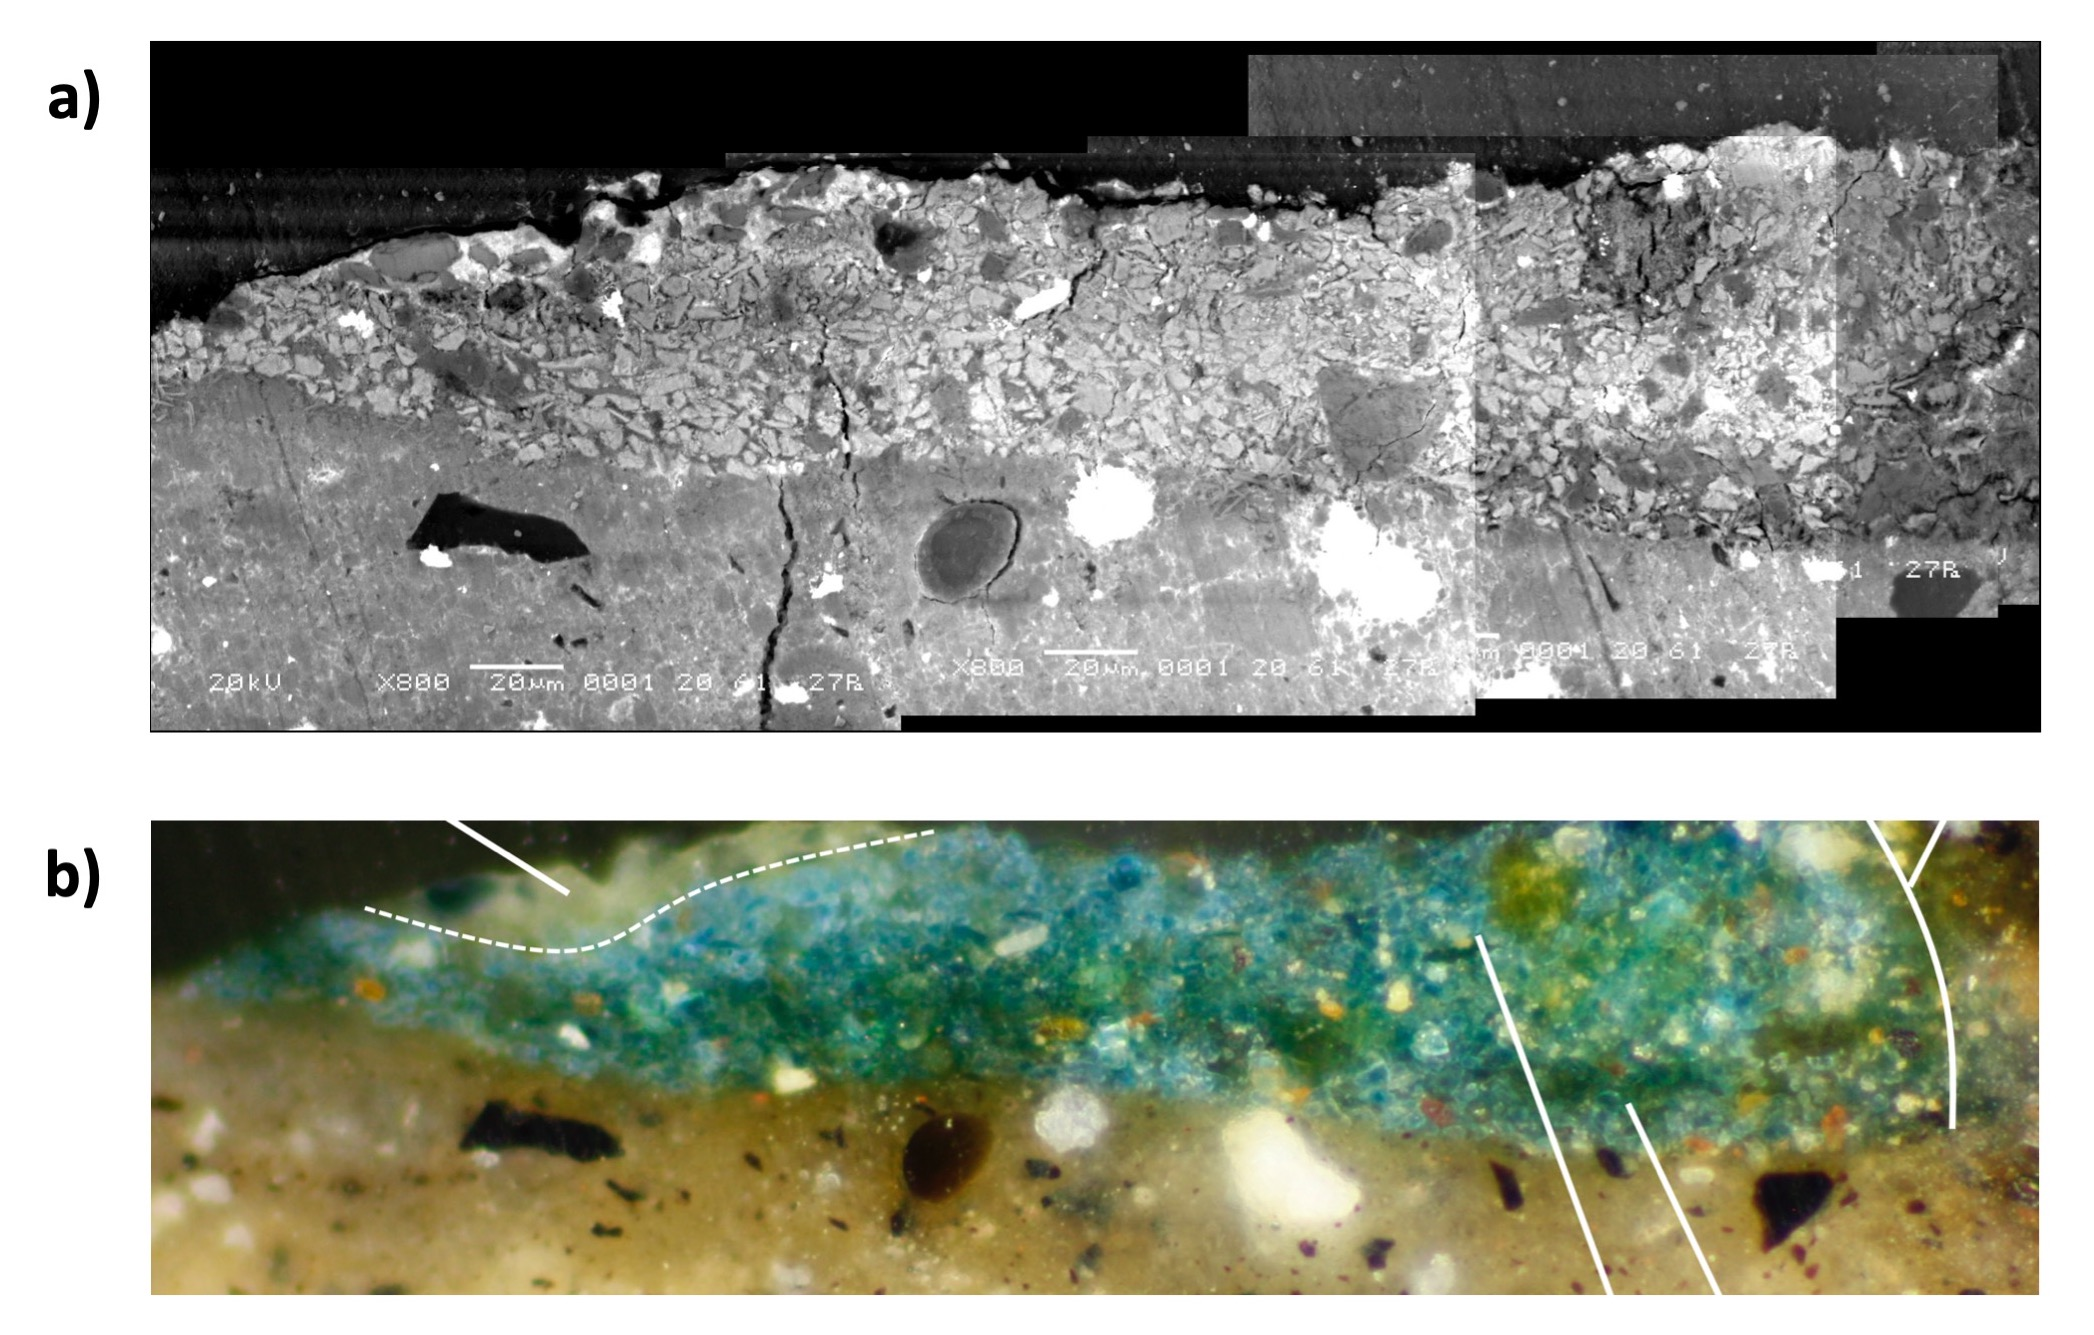
\includegraphics[width=\linewidth]{1259-33_imgs}
\caption[SEM and dark field images of sample 1259.33.]{SEM and dark field images of sample 1259.33: \textbf{a)} composite image of azurite containing layers, 800x magnification, \textbf{b)} dark field microscope image of cross section. Dark field microscope images courtesy of Katharine Waldron, HKI.}
\label{fig:1259.33_imgs}
\end{figure}

\begin{figure}[H]
  \centering
  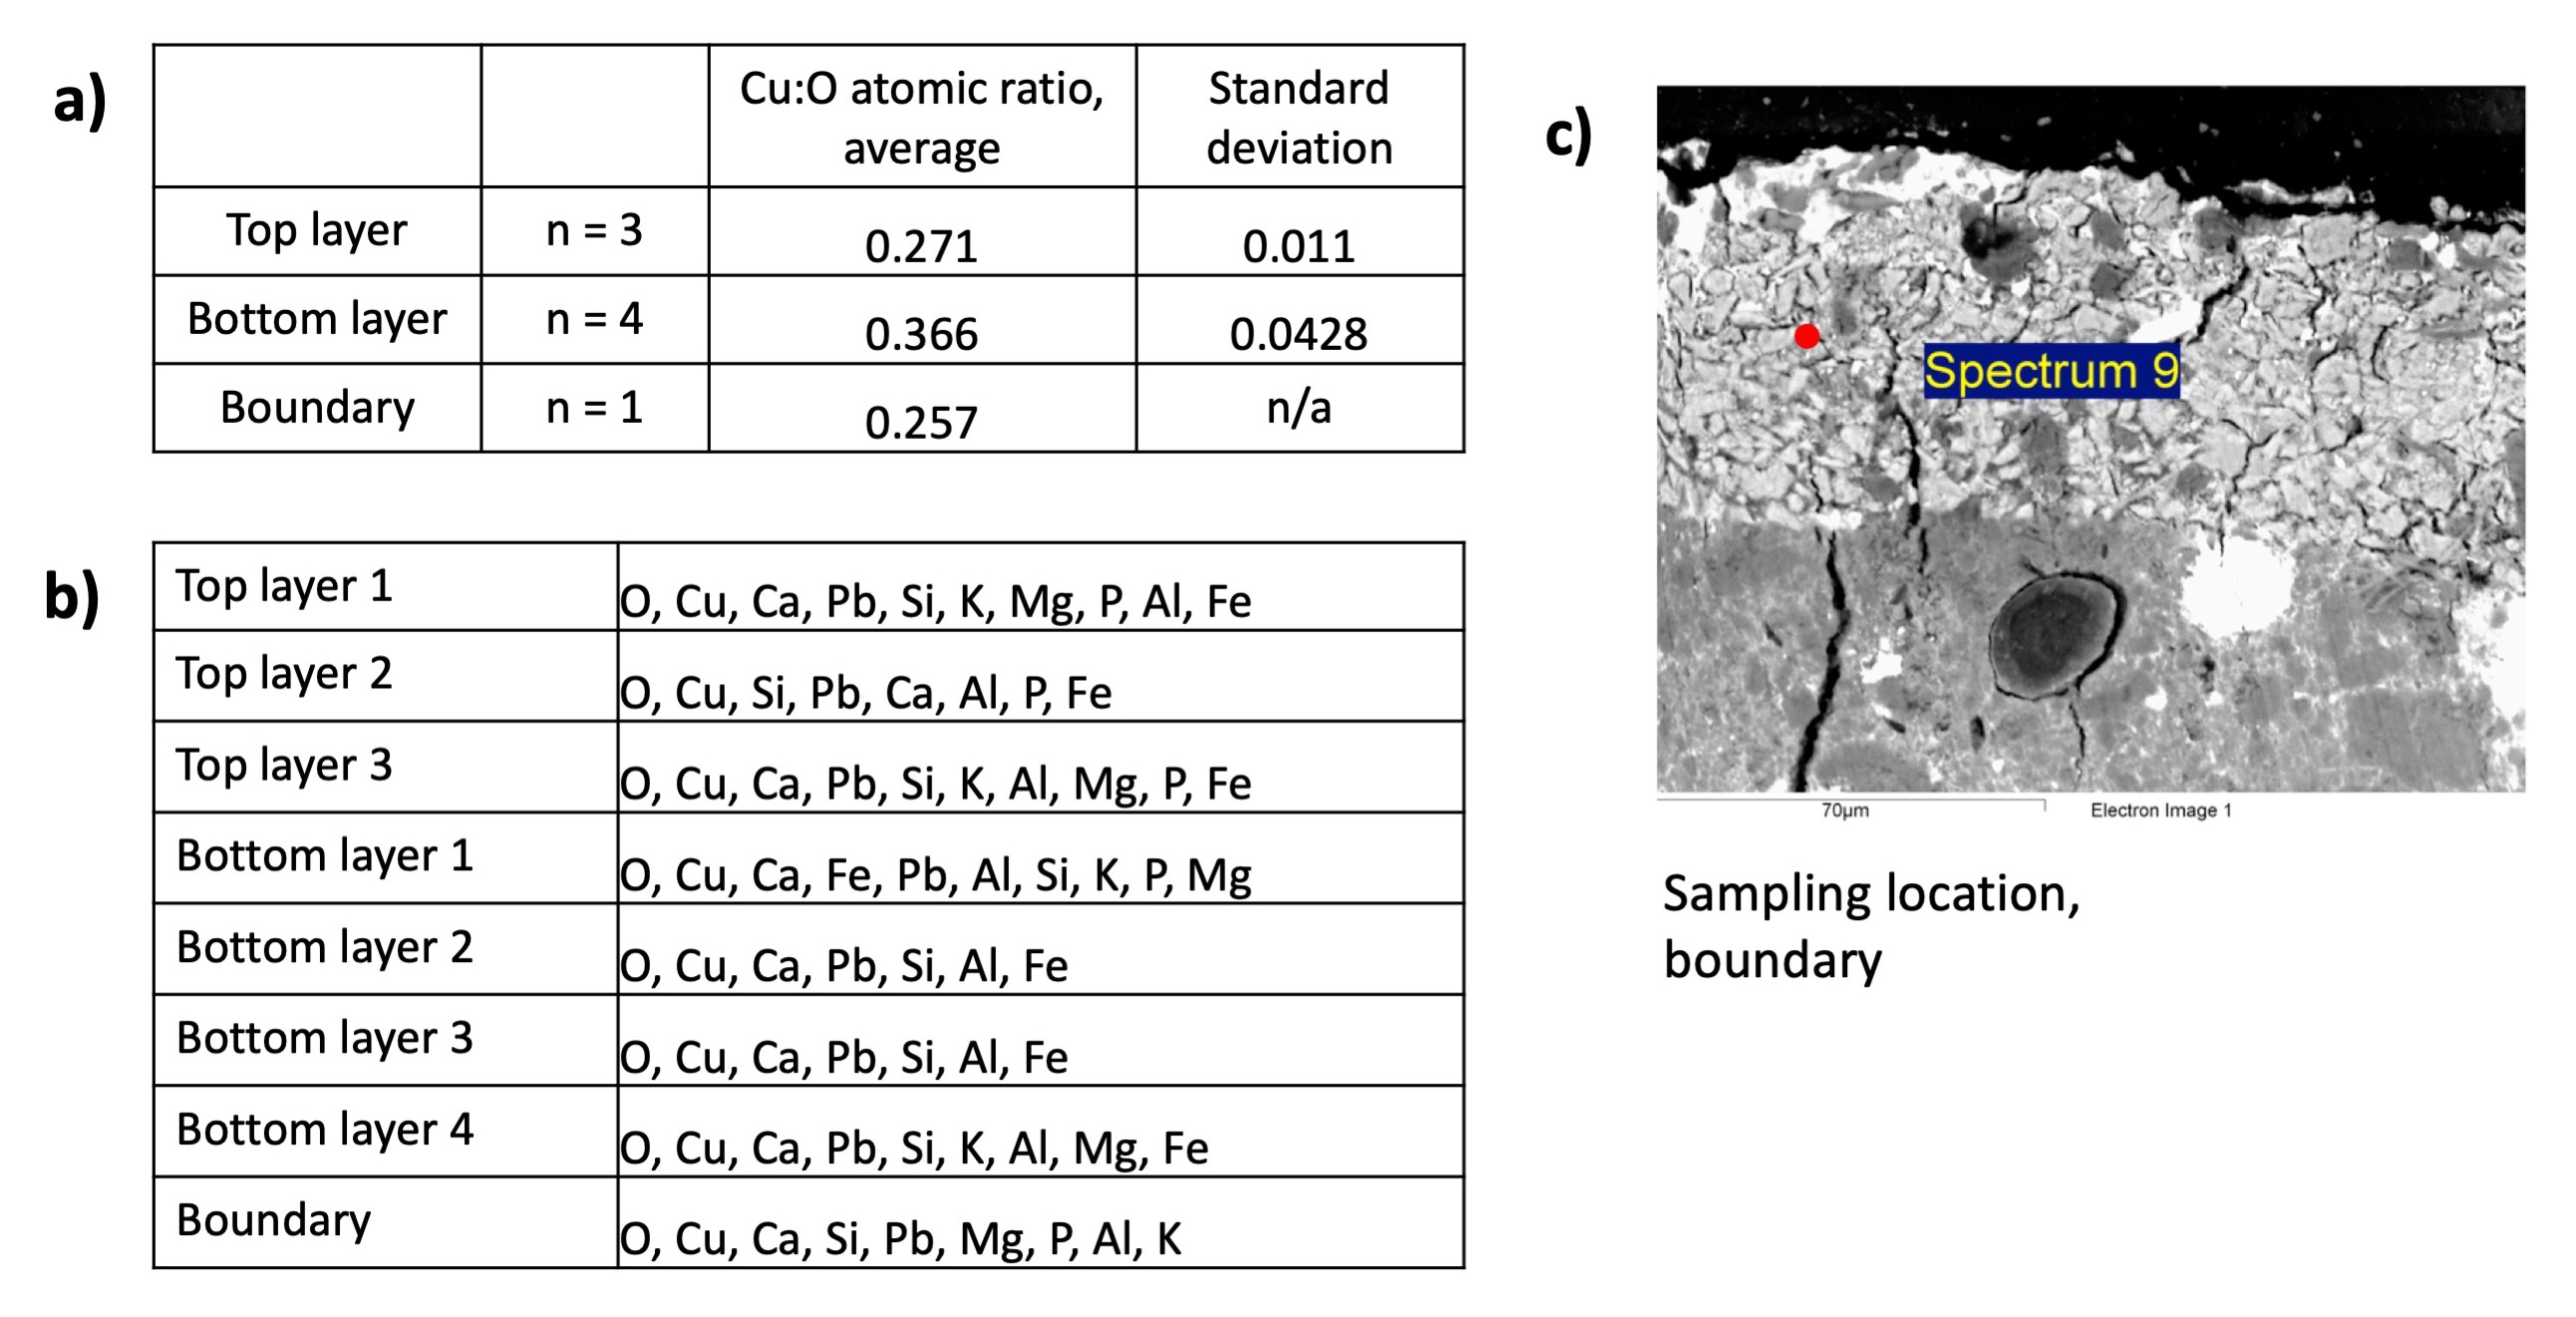
\includegraphics[width=\linewidth]{1259-33_eds_pointspec}
\caption[EDS point spectrum data, sample 1259.33.]{EDS point spectrum data, sample 1259.33: \textbf{a)} quantitative EDS results showing average Cu:O ratio and standard deviation from point spectra collected from azurite particles from the two distinct paint layers in the sample. One sample from the layer boundary is also presented. \textbf{b)} table of elements detected in each point spectrum, \textbf{c)} SEM image showing point spectrum location of boundary sample. This data shows a consistent quantitative difference in the Cu:O ratio between azurite particles in the two paint layers.}
\label{fig:1259.33_pointspec}
\end{figure}

\begin{figure}[H]
\centering
\begin{minipage}[t]{\linewidth}
  \centering
  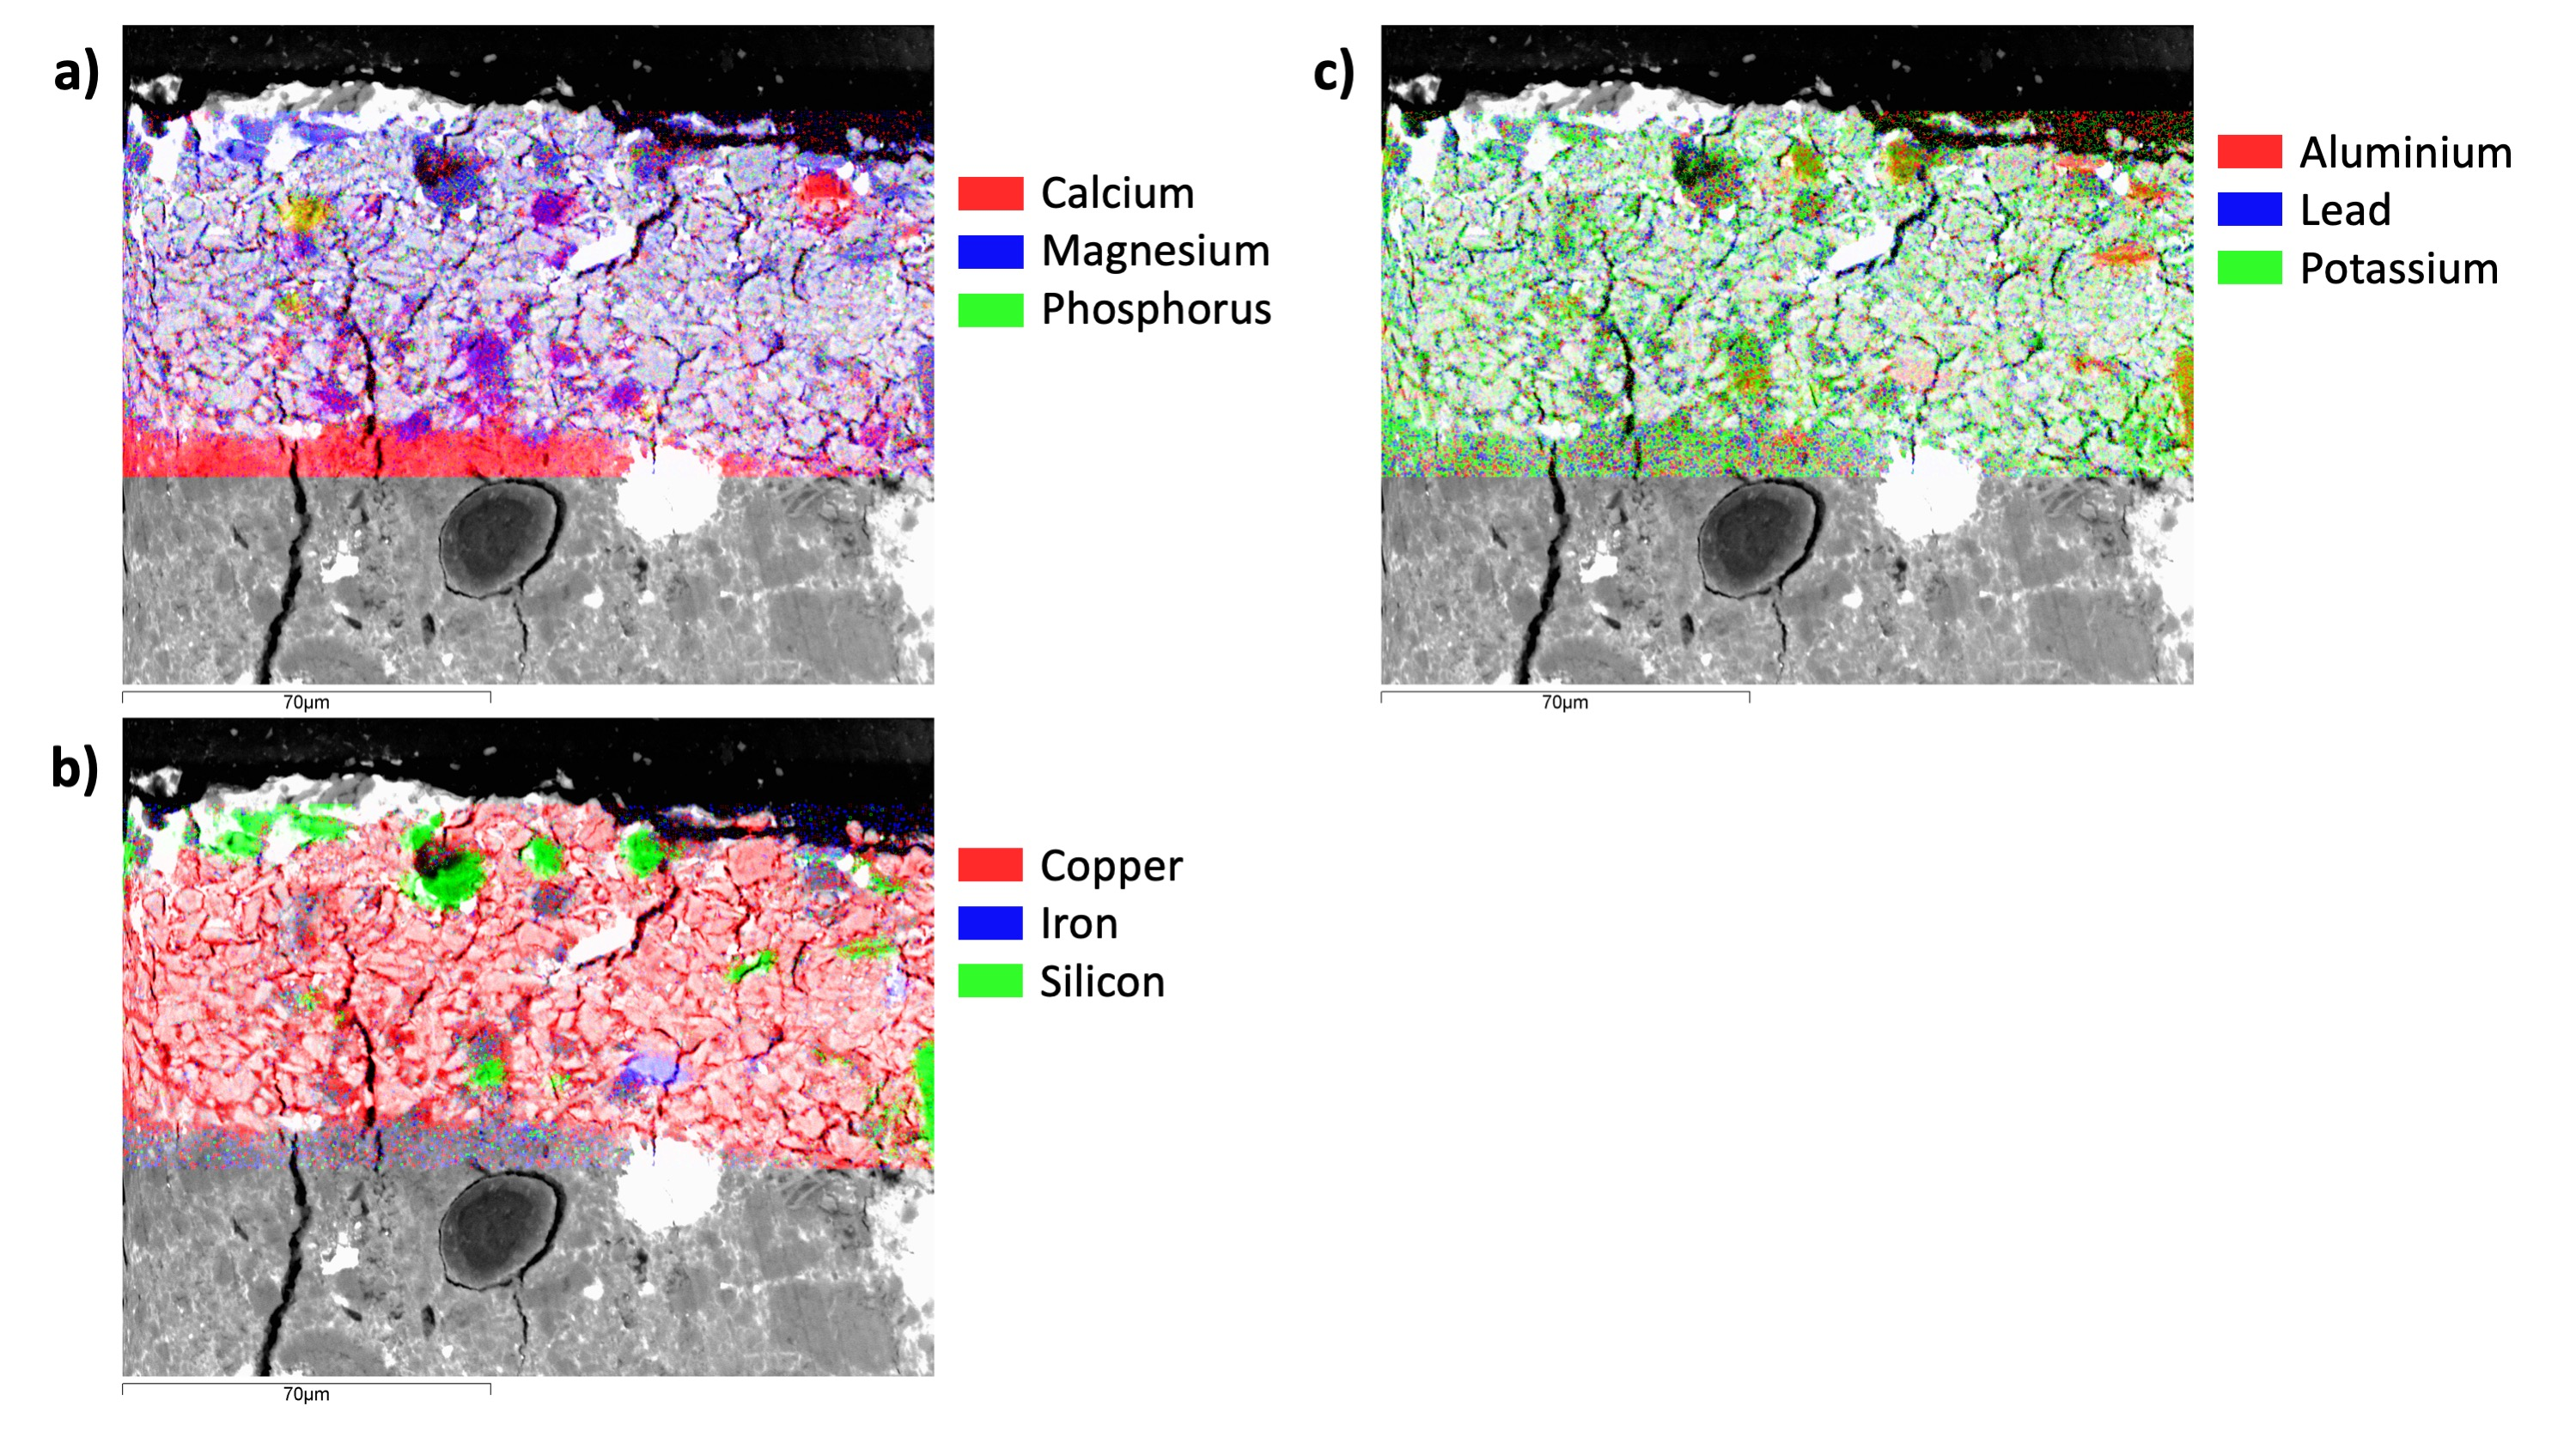
\includegraphics[width=0.9\linewidth]{1259-33_mapdata_1}
\hfill
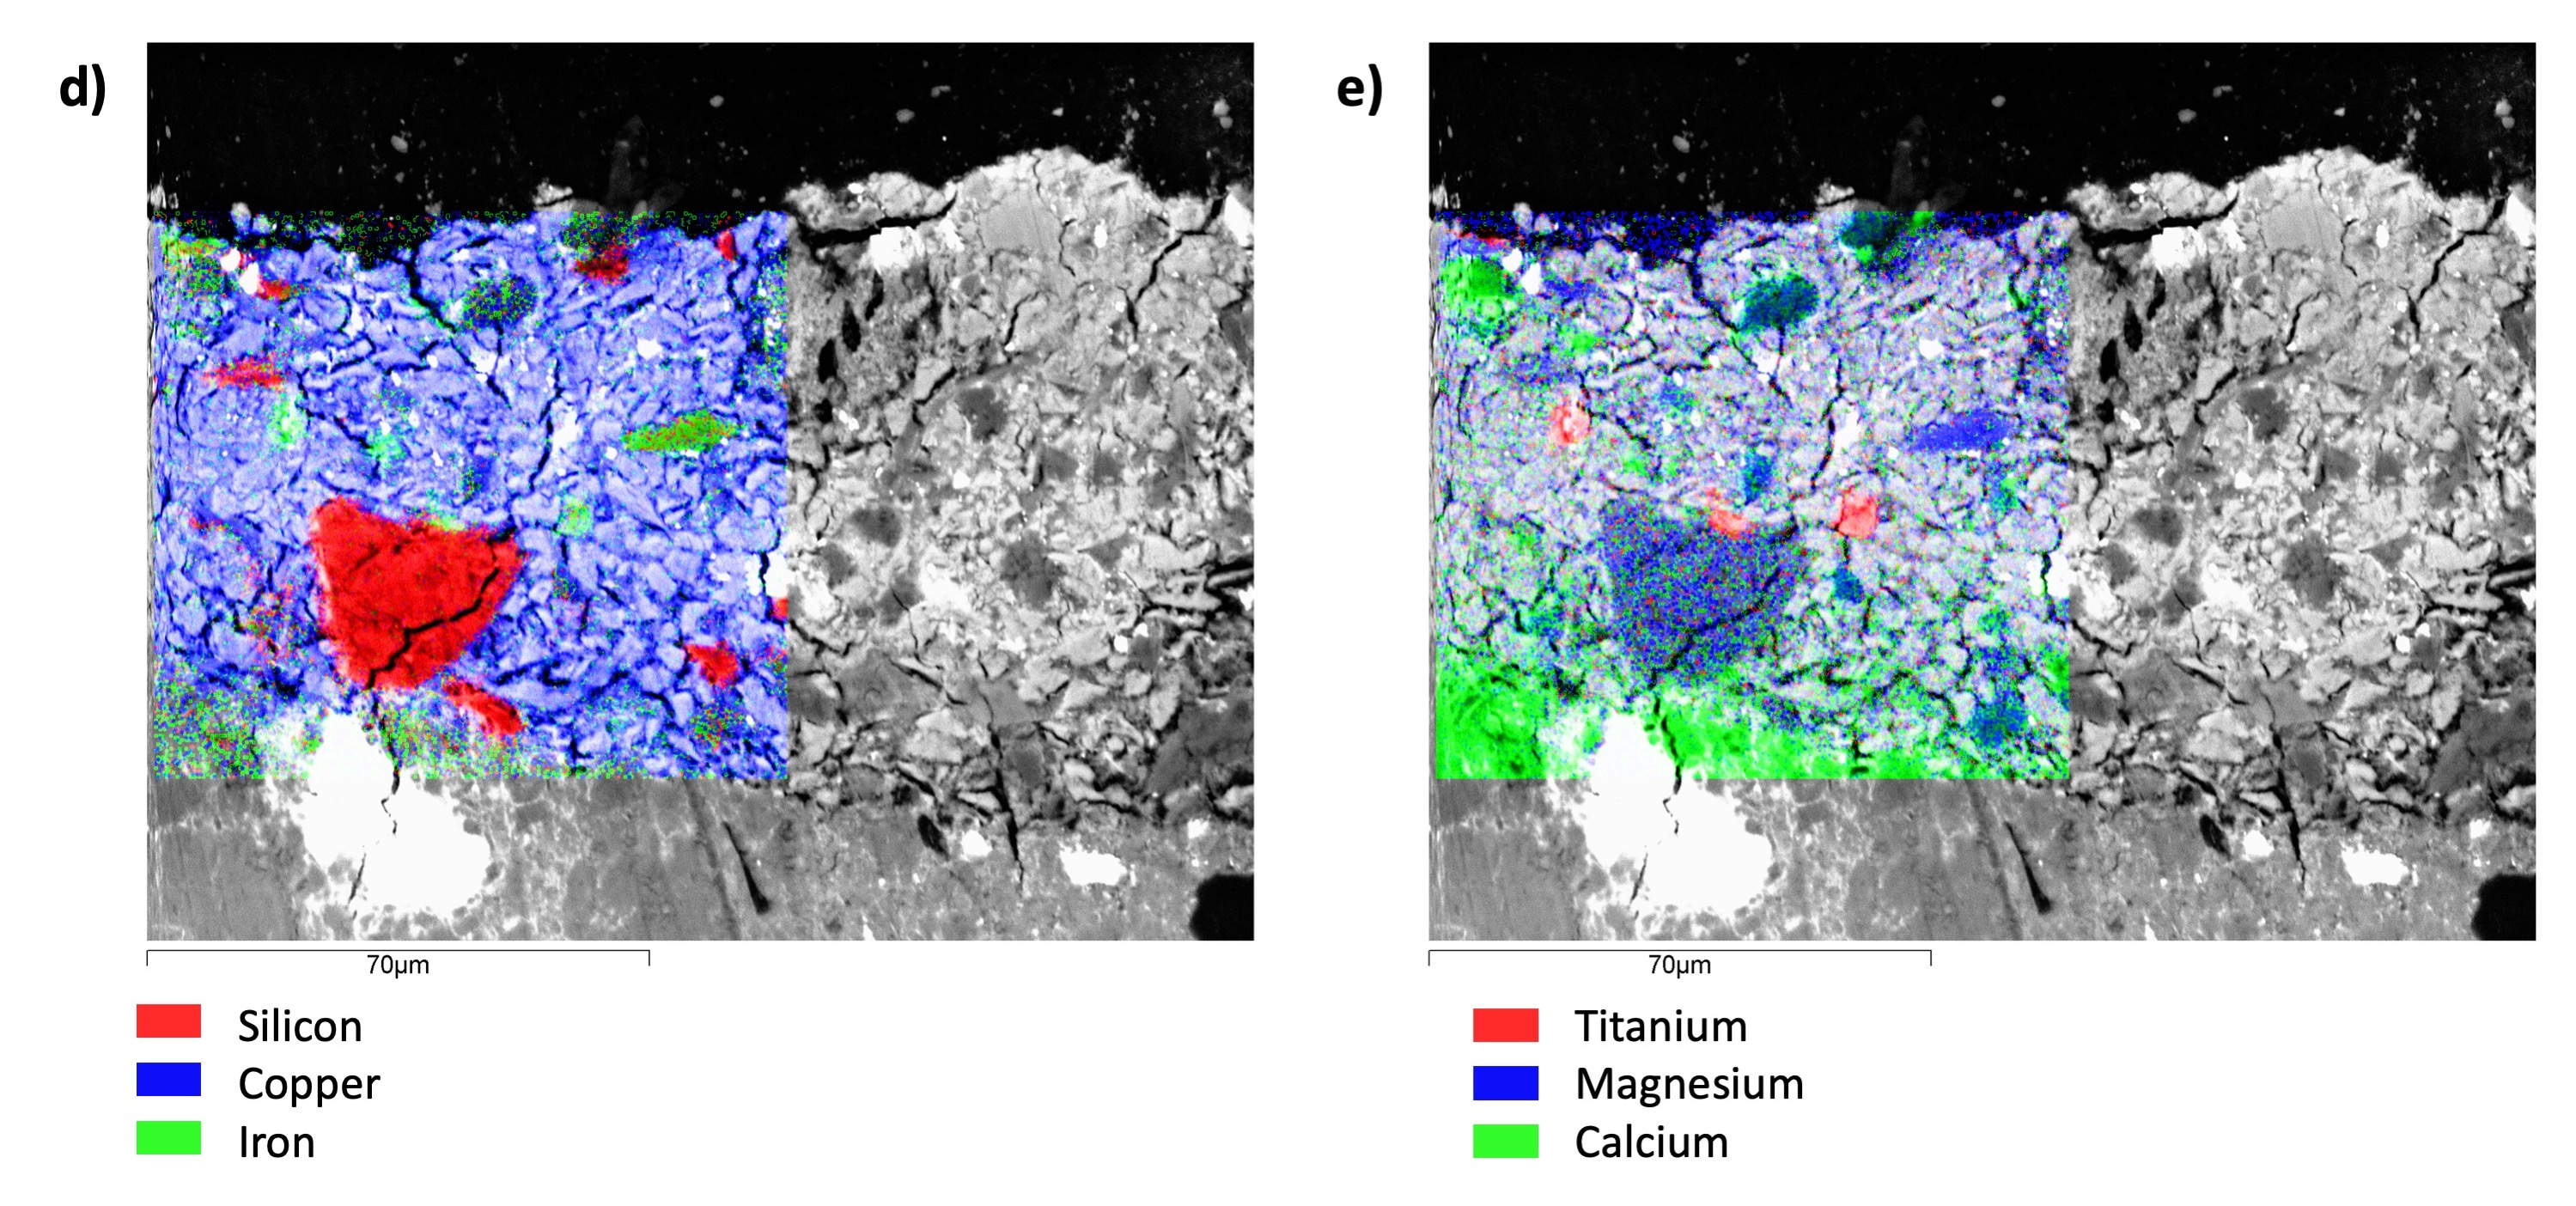
\includegraphics[width=0.9\linewidth]{1259-33_mapdata_2}
\hfill
\end{minipage}
\caption[EDS map data, sample 1259.33.]{EDS map data of sample 1259.33: \textbf{a-c)} elements detected in this region are Ca, Mg, P, Cu, Fe, Si, Al, Pb, K, \textbf{d, e)} elements detected in this region are Si, Cu, Fe, Ti, Mg, Ca.}
\label{fig:1259.33_mapdata}
\end{figure}

\begin{figure}[H]
\centering
  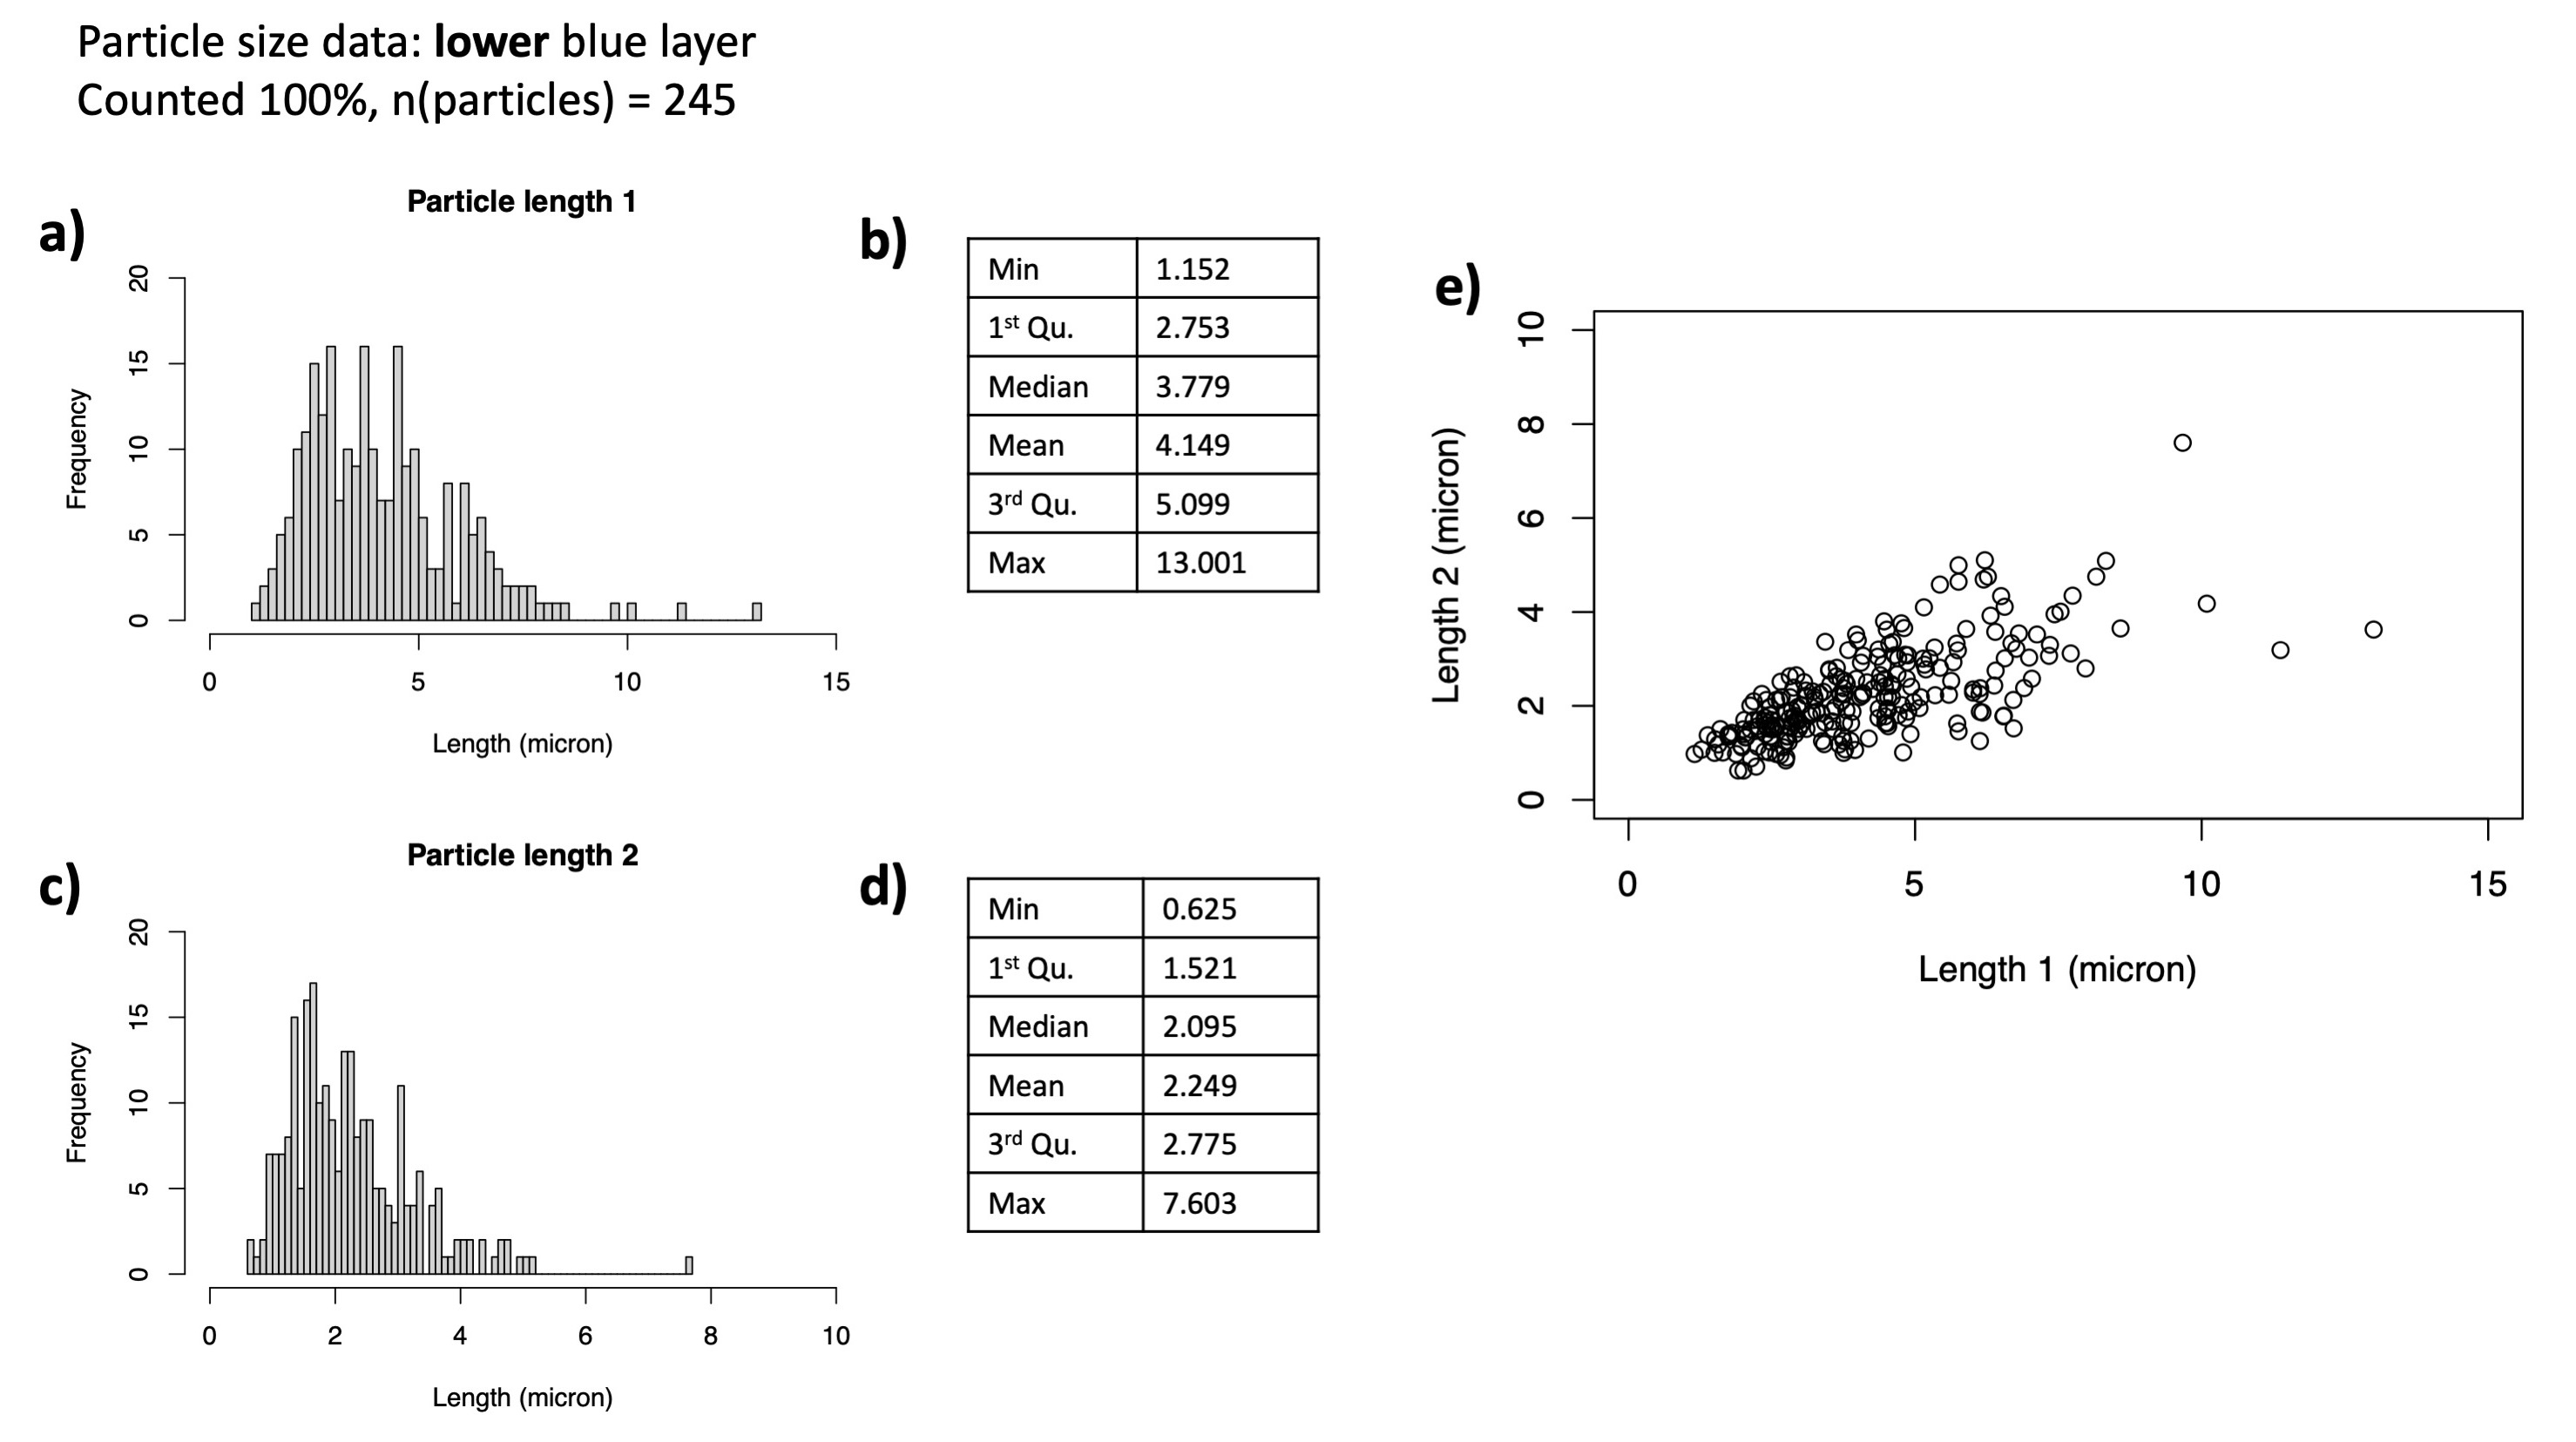
\includegraphics[width=\linewidth]{1259-33_partsize_1}
\caption[Particle size distribution, sample 1259.33, bottom layer.]{Particle size distribution of sample 1259.33, bottom layer: \textbf{a)} Histogram showing distribution of particle length 1 values. \textbf{b)} Descriptive statistics for particle length 1 data. \textbf{c)} Histogram showing distribution of particle length 2 values. \textbf{d)} Descriptive statistics for particle length 2 data. \textbf{e)} Graph of length 1 versus length 2 showing the degree of skew.}
\label{fig:1259.33_partsize_1}
\end{figure}

\begin{figure}[H]
\centering
  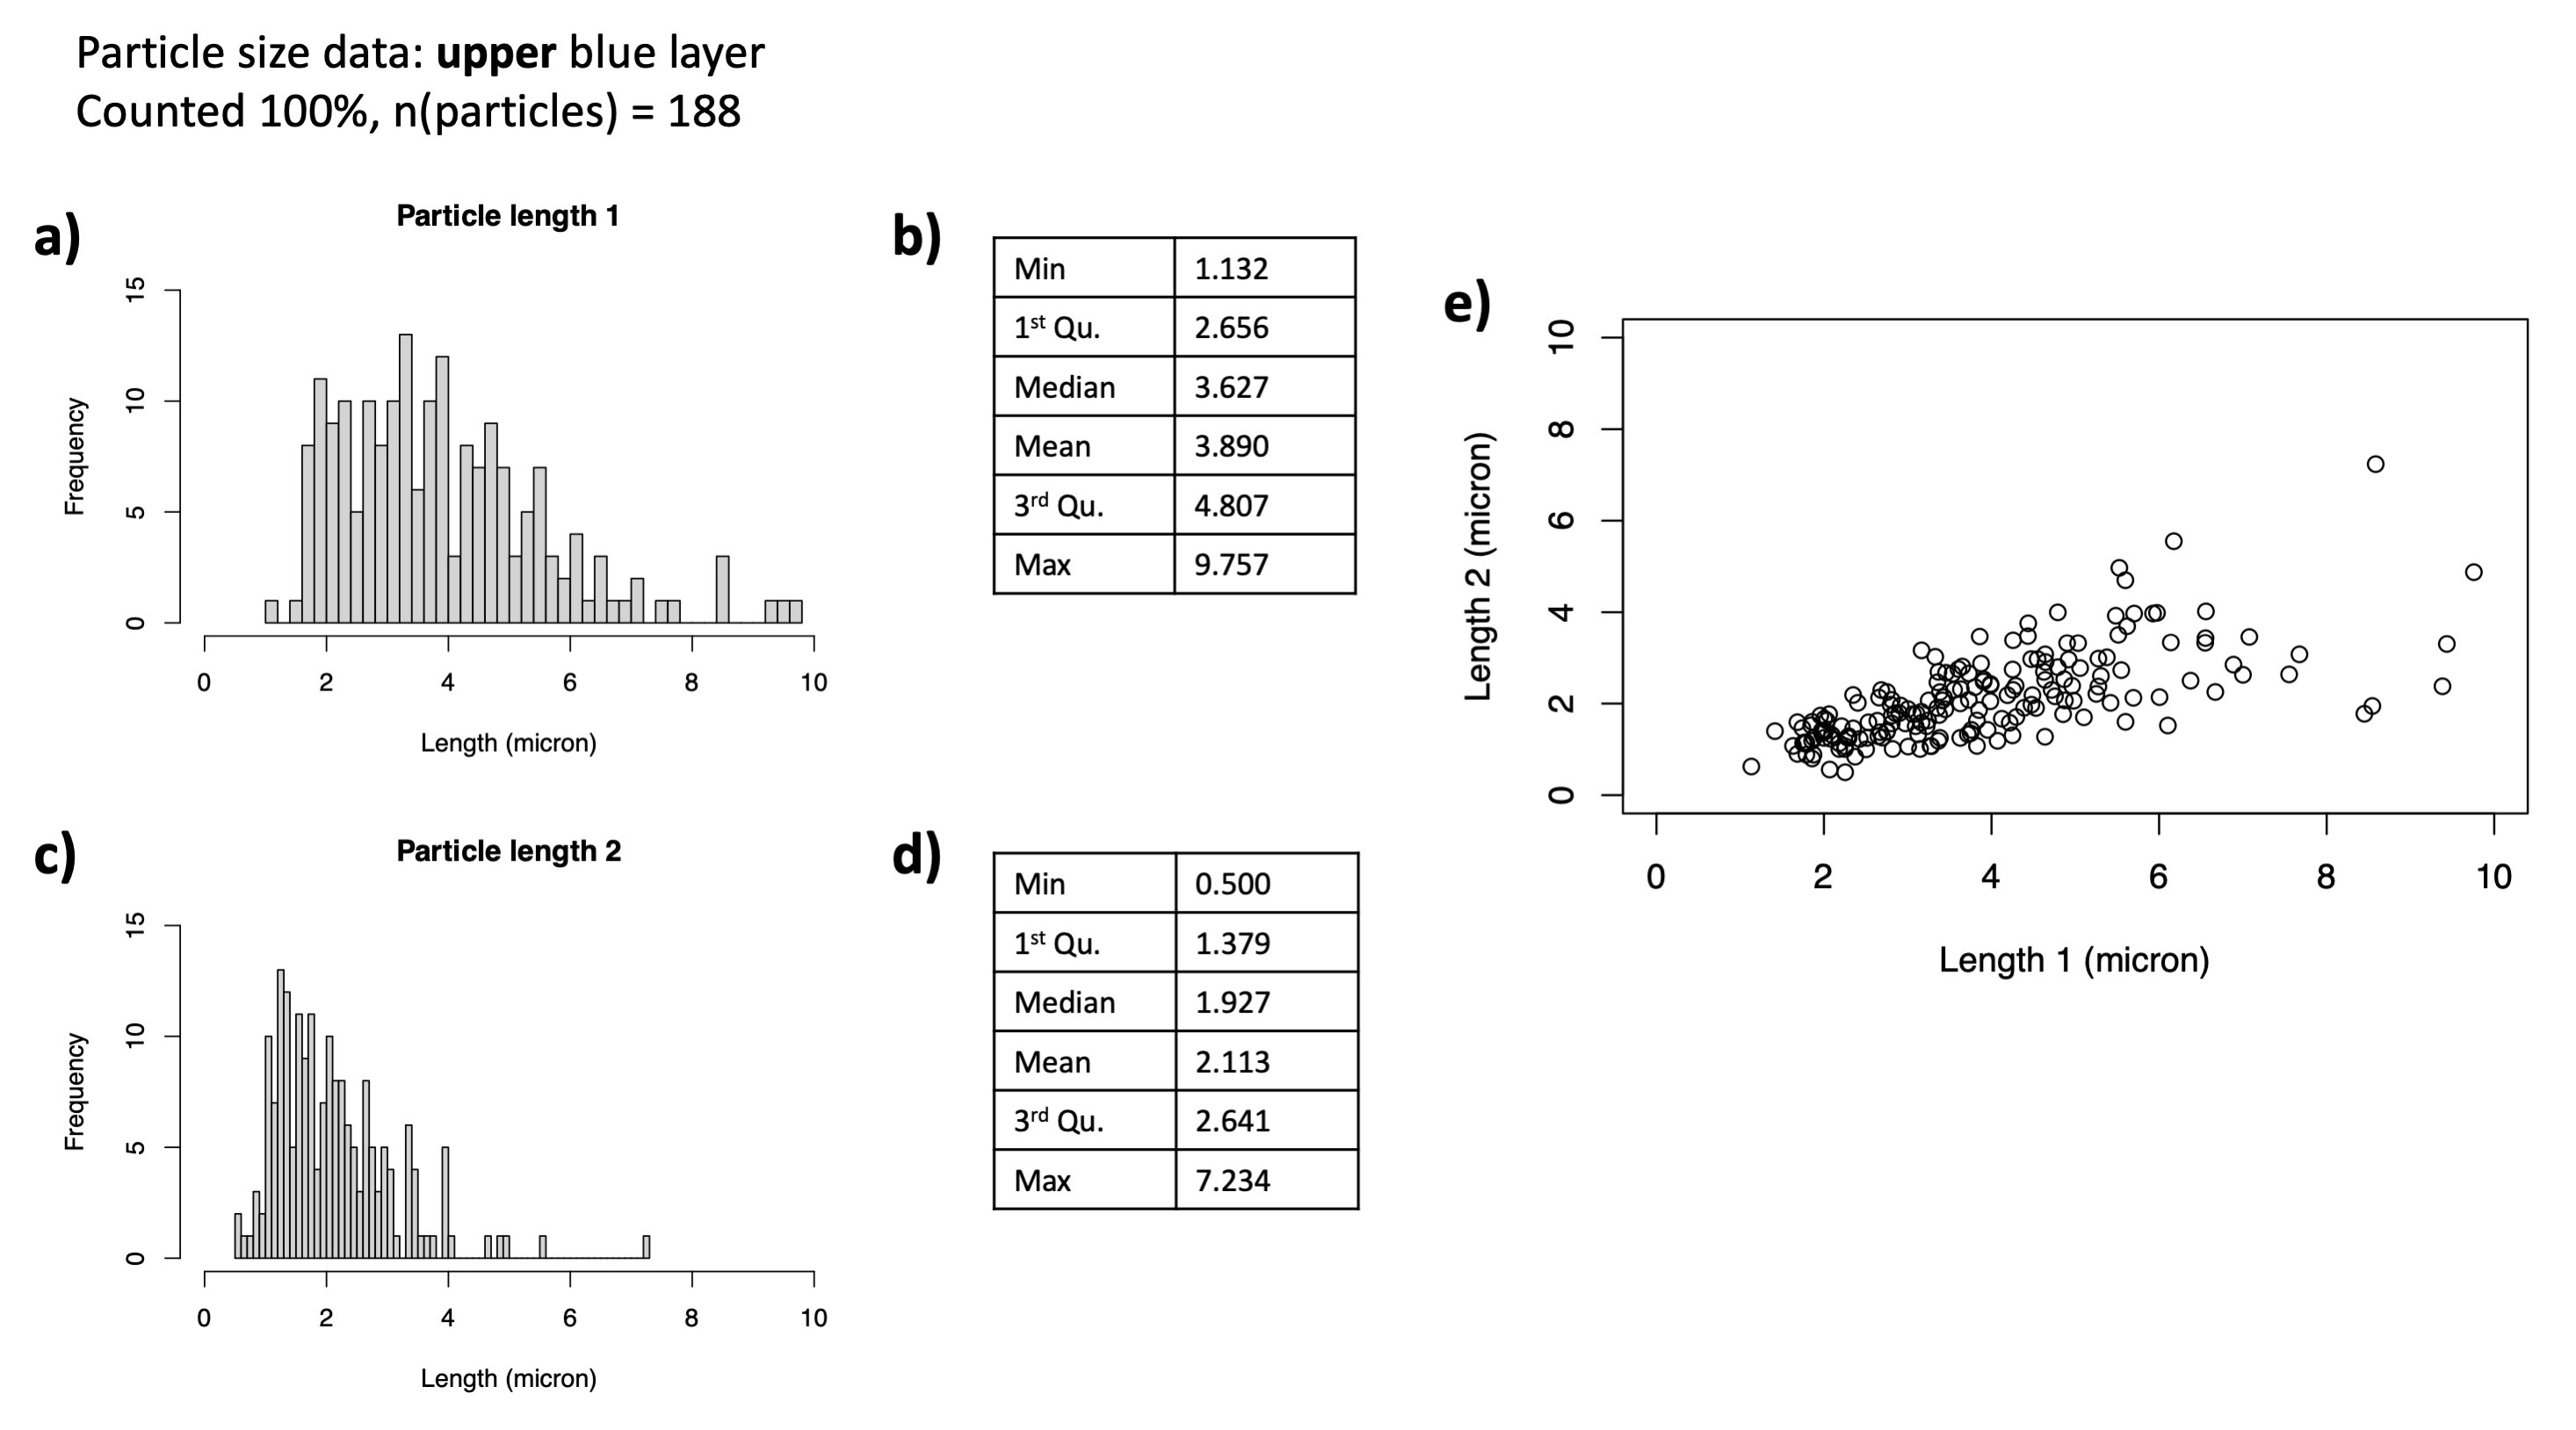
\includegraphics[width=\linewidth]{1259-33_partsize_2}
\caption[Particle size distribution, sample 1259.33, top layer.]{Particle size distribution of sample 1259.33, top layer: \textbf{a)} Histogram showing distribution of particle length 1 values. \textbf{b)} Descriptive statistics for particle length 1 data. \textbf{c)} Histogram showing distribution of particle length 2 values. \textbf{d)} Descriptive statistics for particle length 2 data. \textbf{e)} Graph of length 1 versus length 2 showing the degree of skew.}
\label{fig:1259.33_partsize_2}
\end{figure}


\section{Sample 1259.34}

\textit{Figure \ref{fig:1259.34_imgs}} shows SEM and dark field microscope images of 1259.34, with two distinct original azurite-containing layers. One of these contains a large proportion of white pigment mixed with azurite. EDS mapping (\textit{Figure \ref{fig:1259.34_mapdata}}) shows azurite, iron oxide, aluminosilicates including feldspar, rutile, and dolomite (CaMg(CO\textsubscript{3})\textsubscript{2}). Only the top layer contains lead and arsenic, likely cerussite (lead white).

\textit{Figures \ref{fig:1259.34_partsize_2}} and \textit{\ref{fig:1259.34_partsize_1}} show particle size data for the bottom and top layers containing azurite. These layers do not differ except a small number of outlying large particles in the bottom layer, and both contain small pigments with approximate average dimensions length 1 = 2(length2). 

\begin{figure}[H]
  \centering
  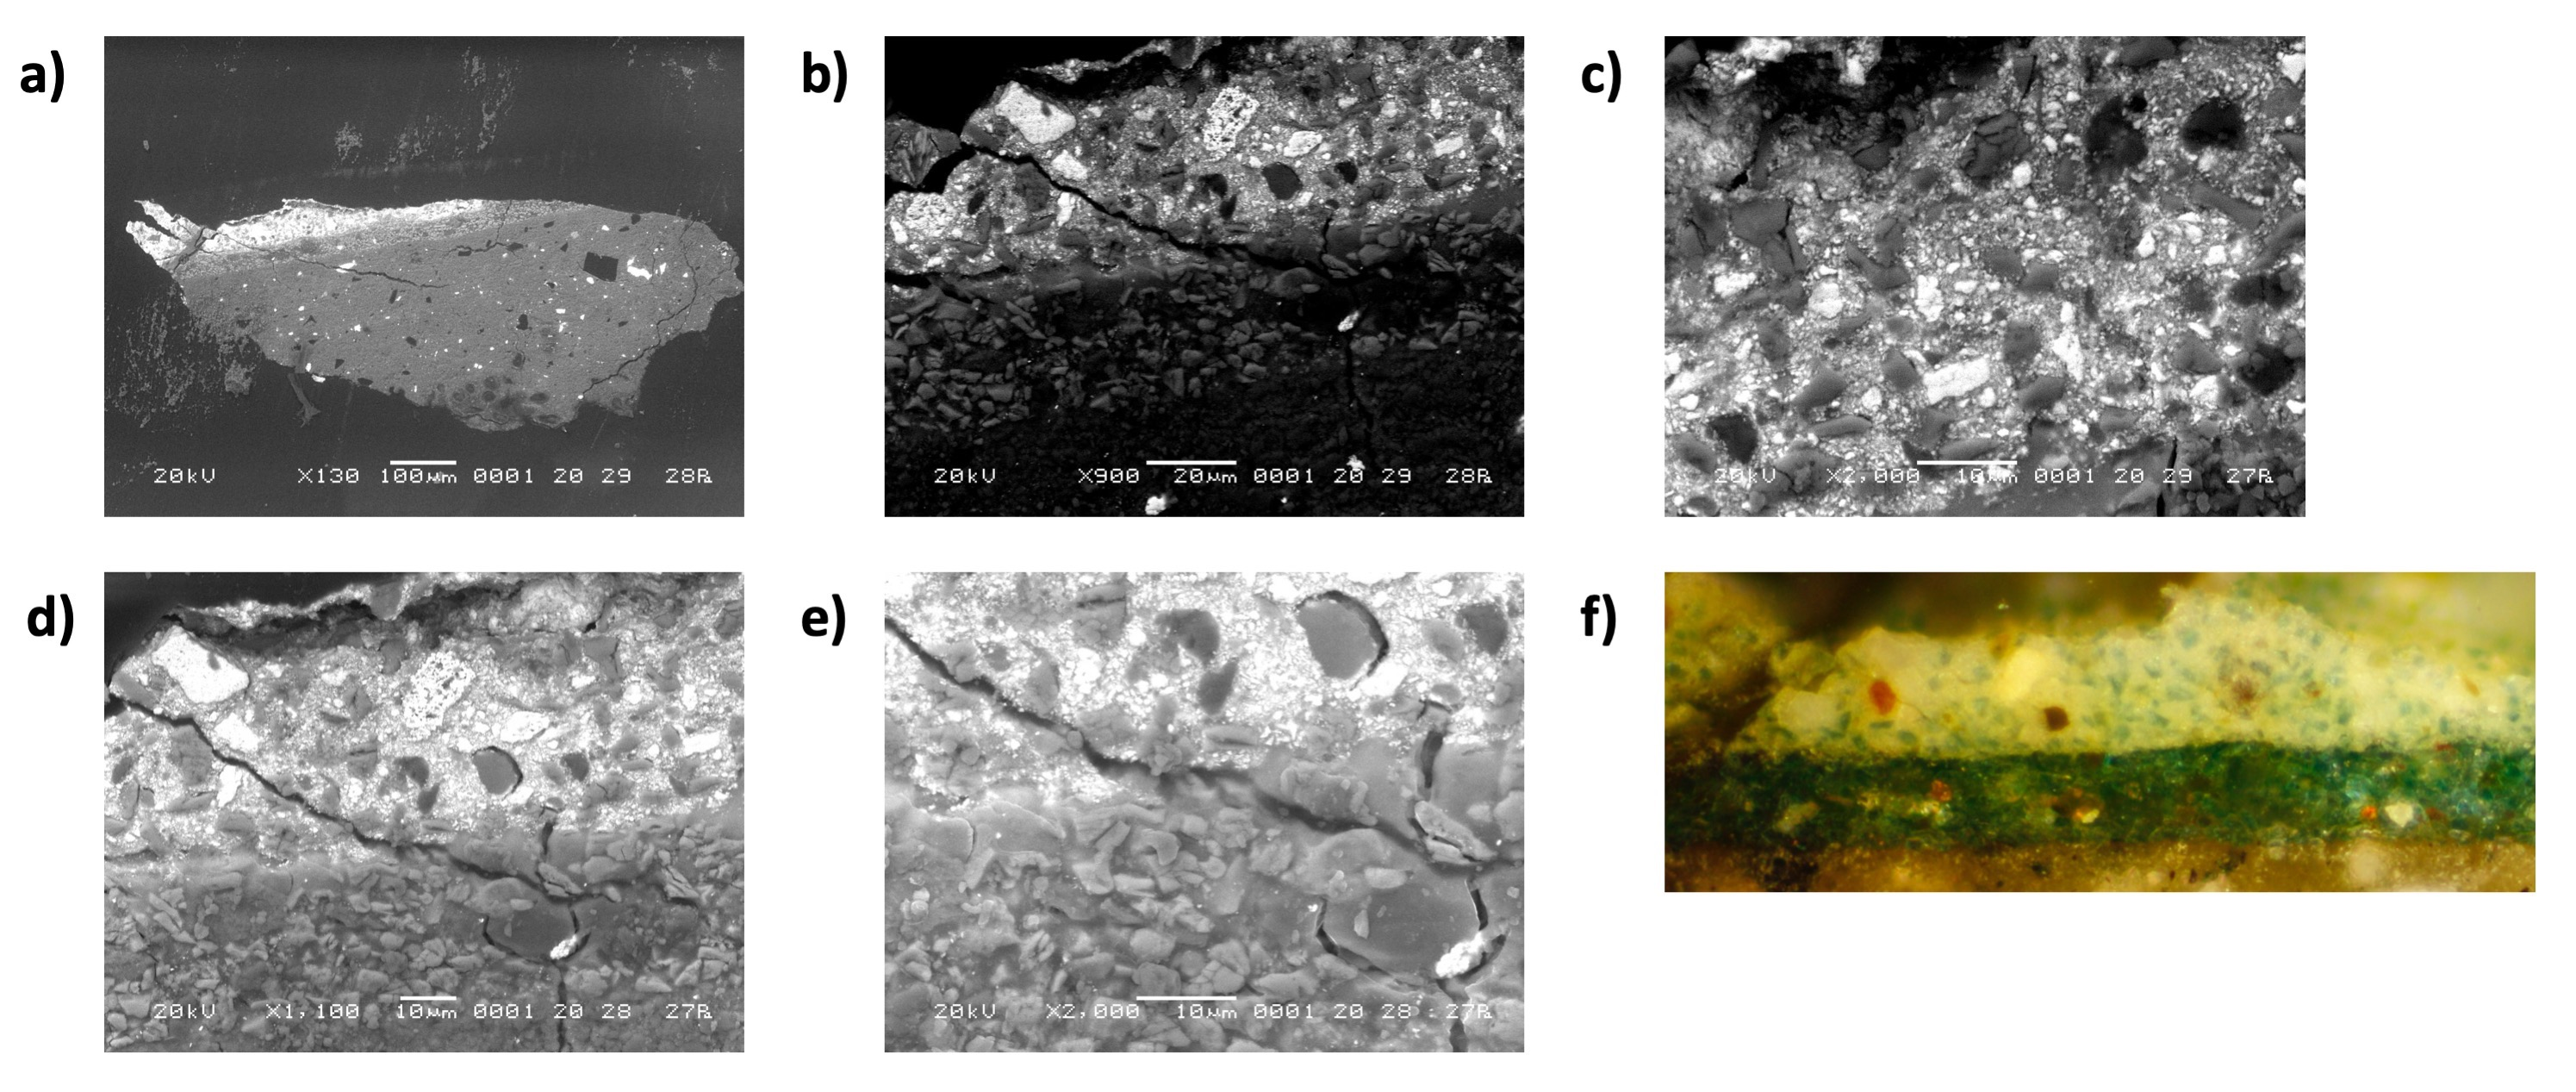
\includegraphics[width=\linewidth]{1259-34_imgs}
\caption[SEM and dark field images of sample 1259.34.]{SEM and dark field images of sample 1259.34: \textbf{a)} 130x magnification showing two distinct layers containing azurite (both original), \textbf{b)} 900x magnification, \textbf{c)} 2000x magnification, \textbf{d)} 1100x magnification, \textbf{e)} 2000x magnification, \textbf{f)} dark field microscope image showing two distinct layers. Dark field microscope images courtesy of Katharine Waldron, HKI.}
\label{fig:1259.34_imgs}
\end{figure}

\begin{figure}[H]
\centering
\begin{minipage}[t]{\linewidth}
  \centering
  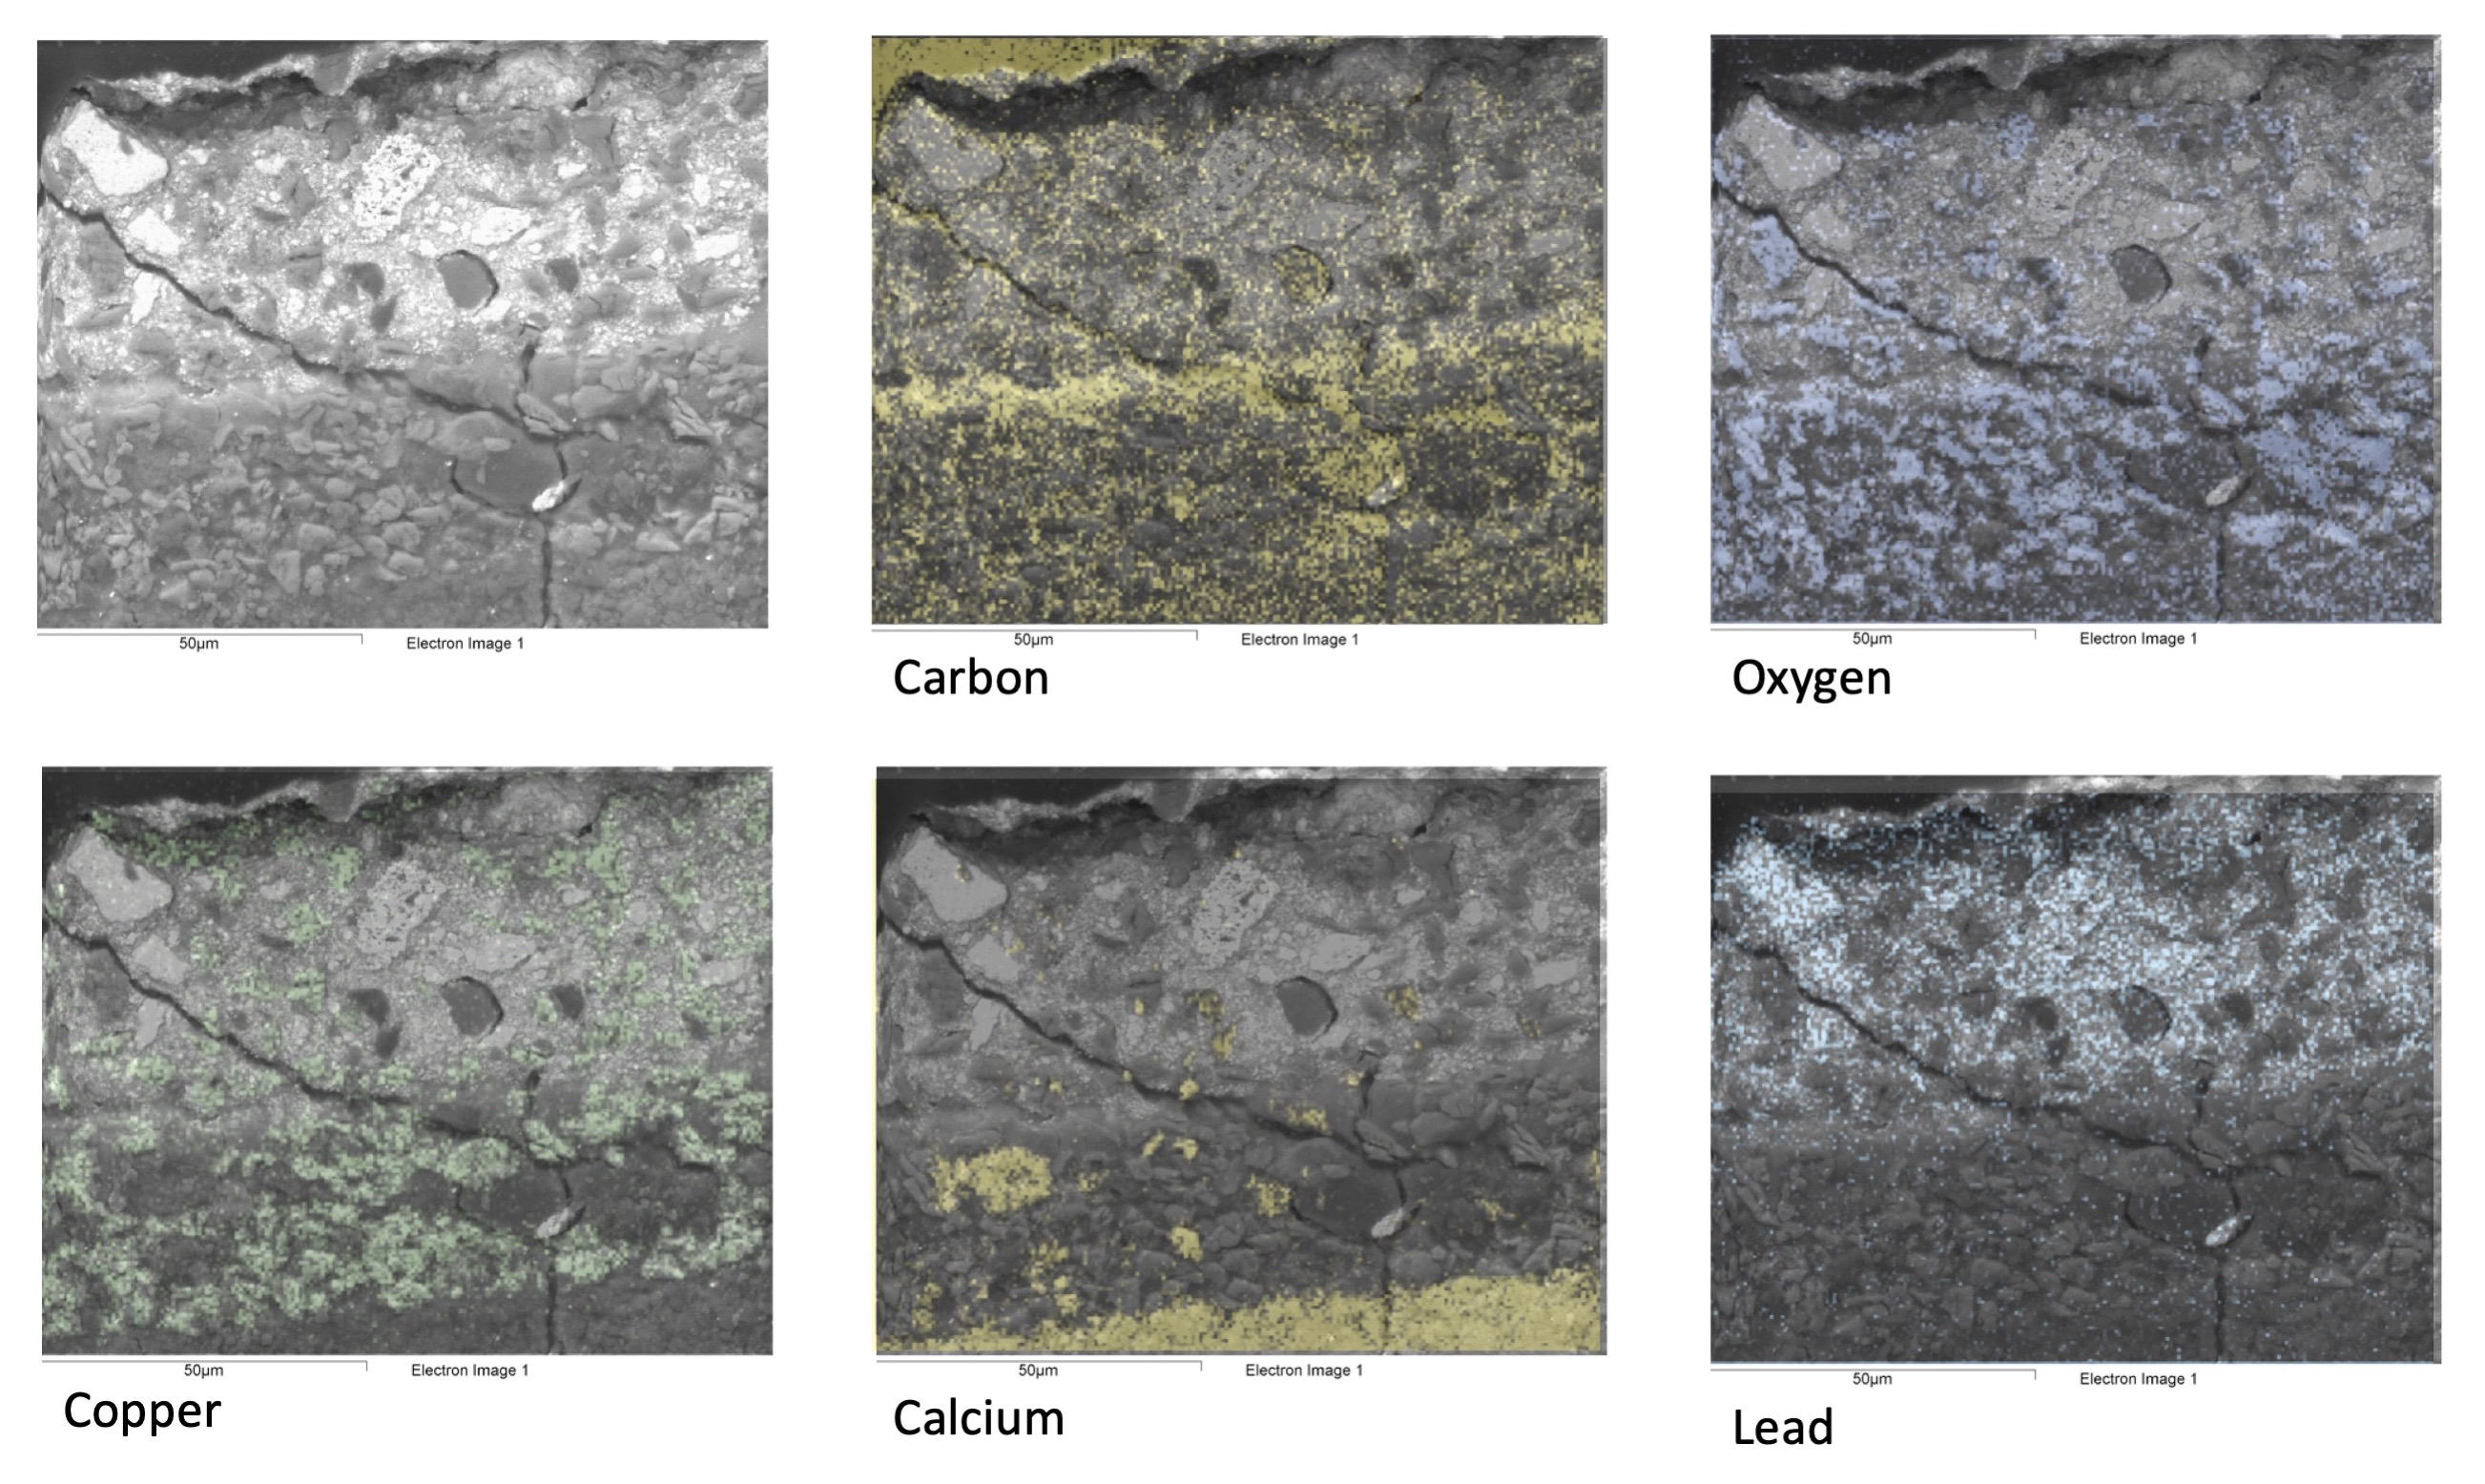
\includegraphics[width=0.9\linewidth]{1259-34_mapdata_1}
\hfill
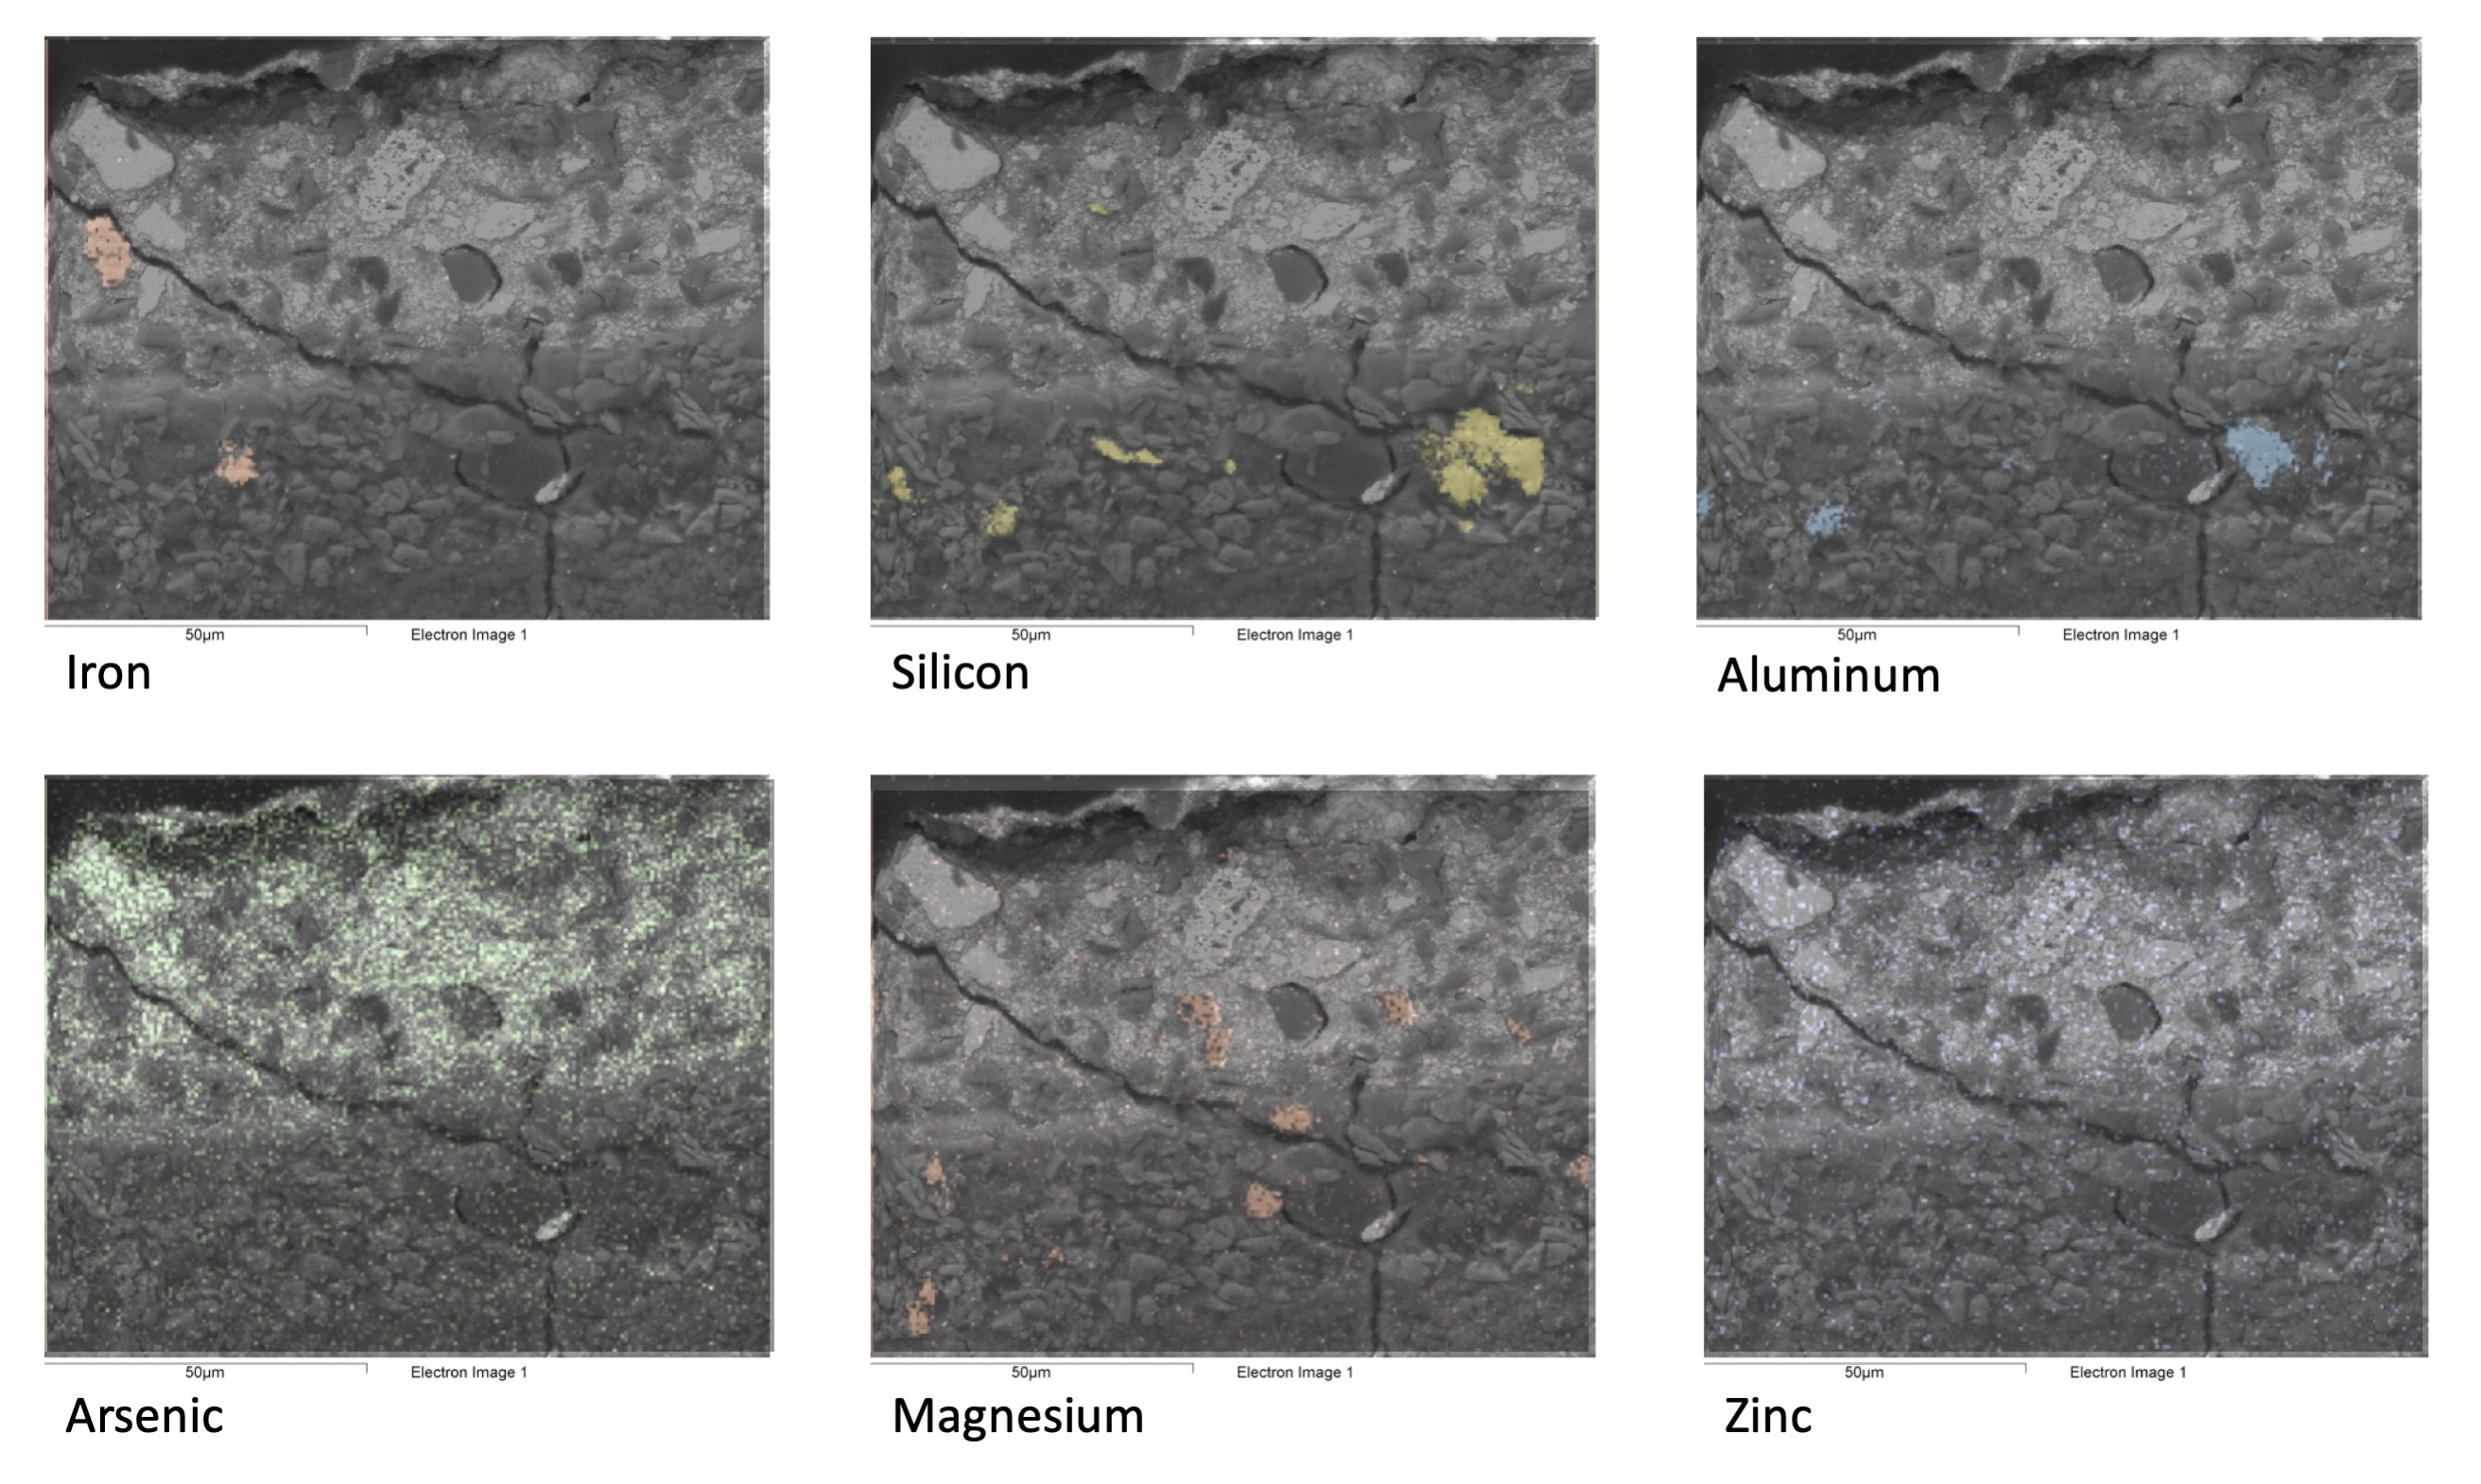
\includegraphics[width=0.9\linewidth]{1259-34_mapdata_2}
\hfill
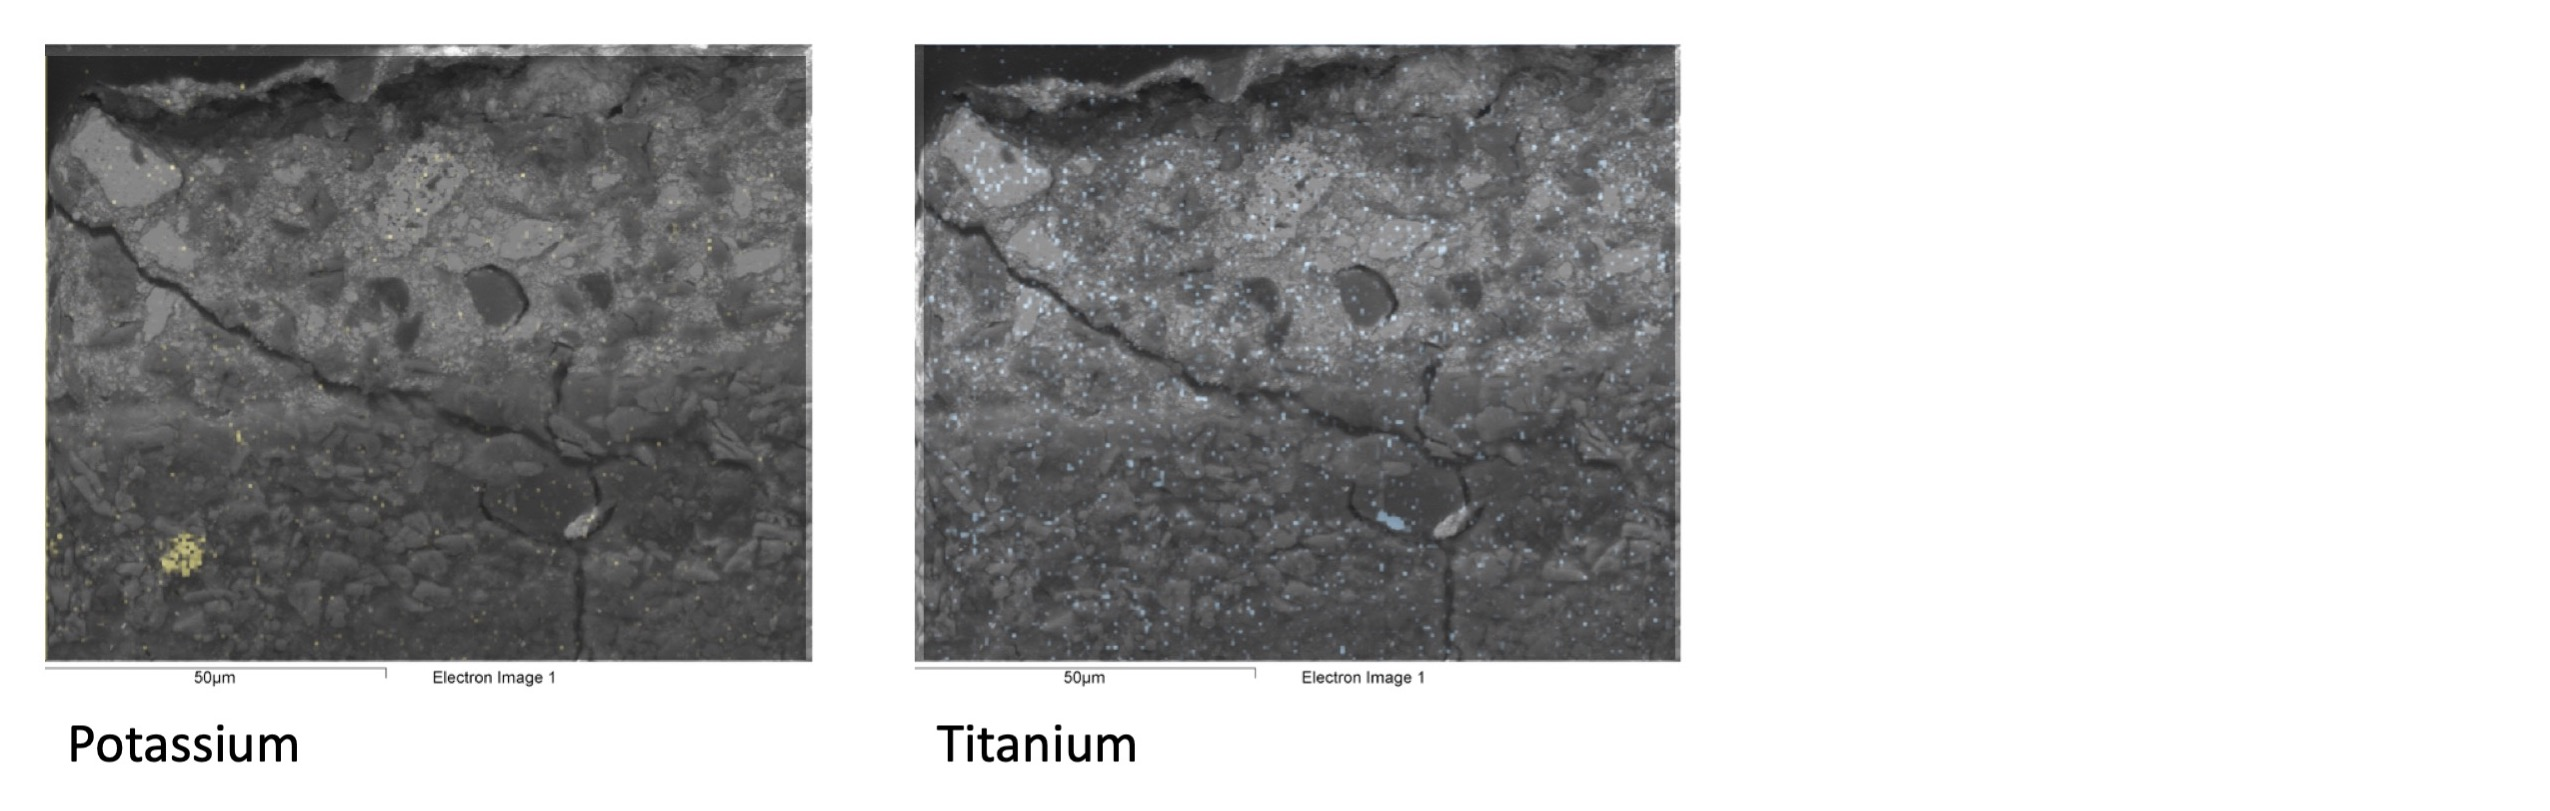
\includegraphics[width=0.9\linewidth]{1259-34_mapdata_3}
\hfill
\end{minipage}
\caption[EDS map data, sample 1259.34.]{EDS map data of sample 1259.34 showing locations of elements in both azurite-containing layers. Elements detected are C, O, Cu, Ca, Pb, Fe, Si, Al, As, Mg, Zn, K, and Ti.}
\label{fig:1259.34_mapdata}
\end{figure}

\begin{figure}[H]
\centering
  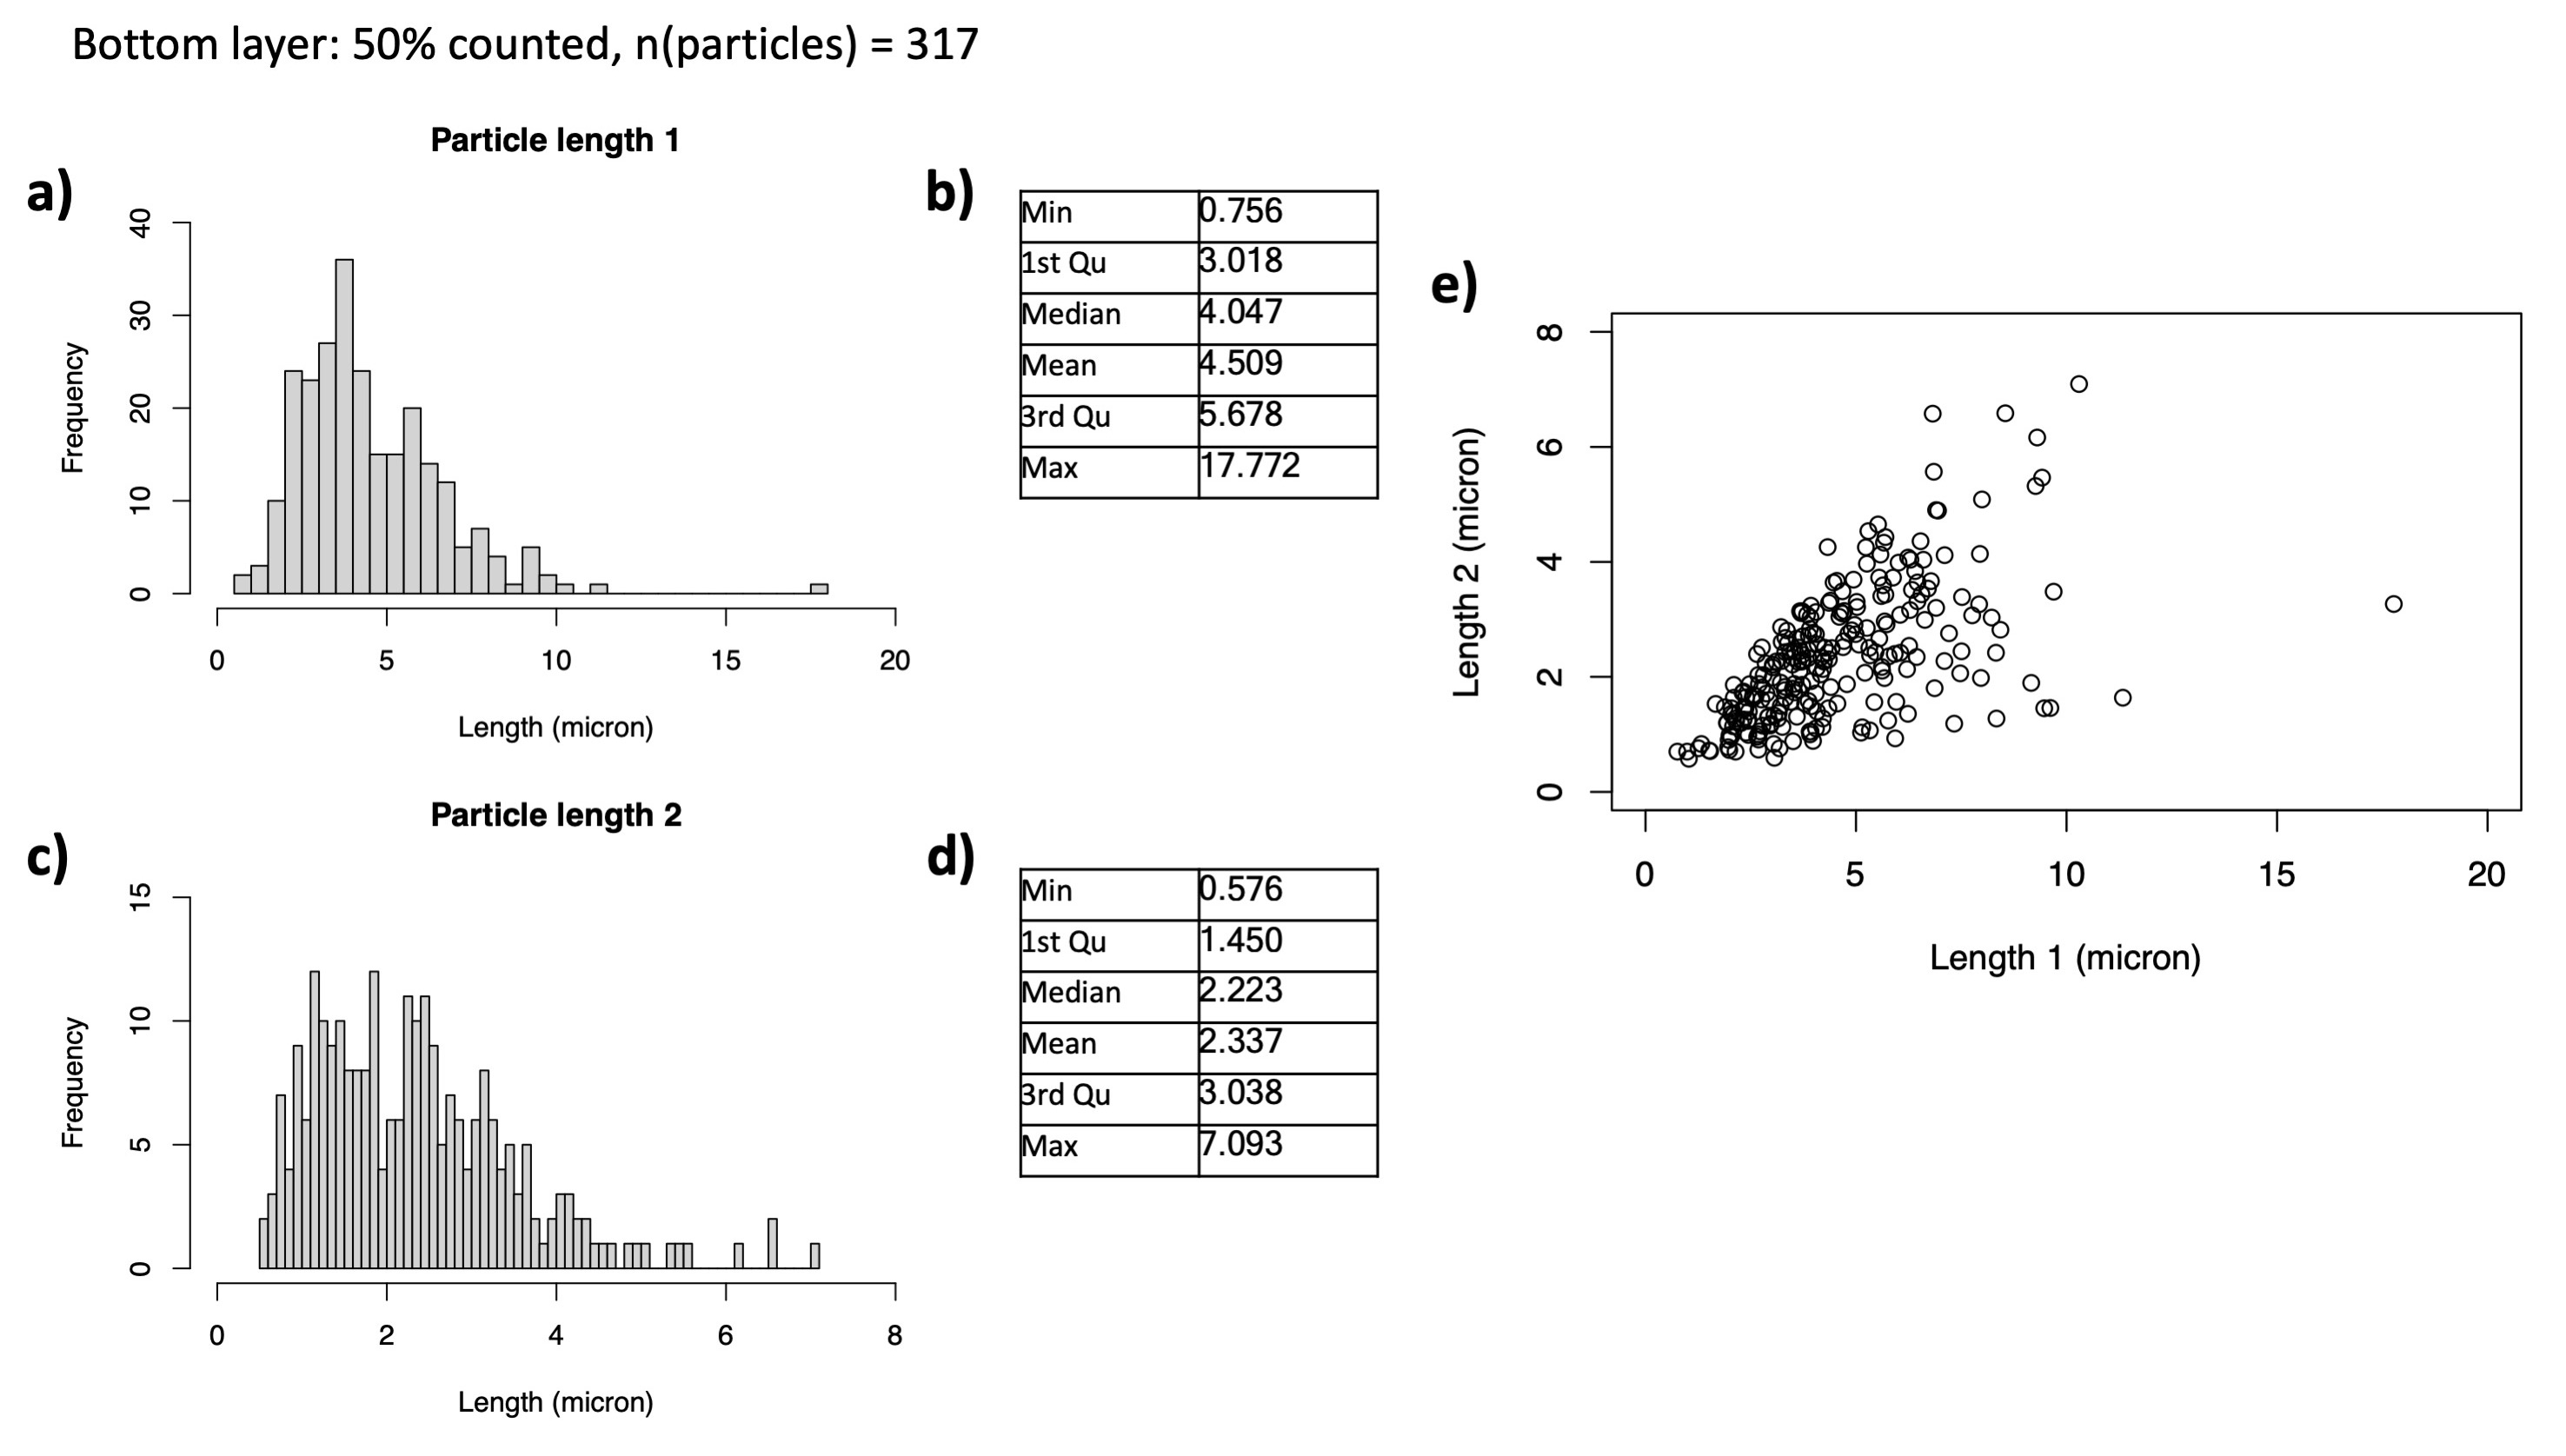
\includegraphics[width=\linewidth]{1259-34_partsize_2}
\caption[Particle size distribution, sample 1259.34, bottom layer.]{Particle size distribution of sample 1259.34, bottom layer: \textbf{a)} Histogram showing distribution of particle length 1 values. \textbf{b)} Descriptive statistics for particle length 1 data. \textbf{c)} Histogram showing distribution of particle length 2 values. \textbf{d)} Descriptive statistics for particle length 2 data. \textbf{e)} Graph of length 1 versus length 2 showing the degree of skew.}
\label{fig:1259.34_partsize_2}
\end{figure}

\begin{figure}[H]
\centering
  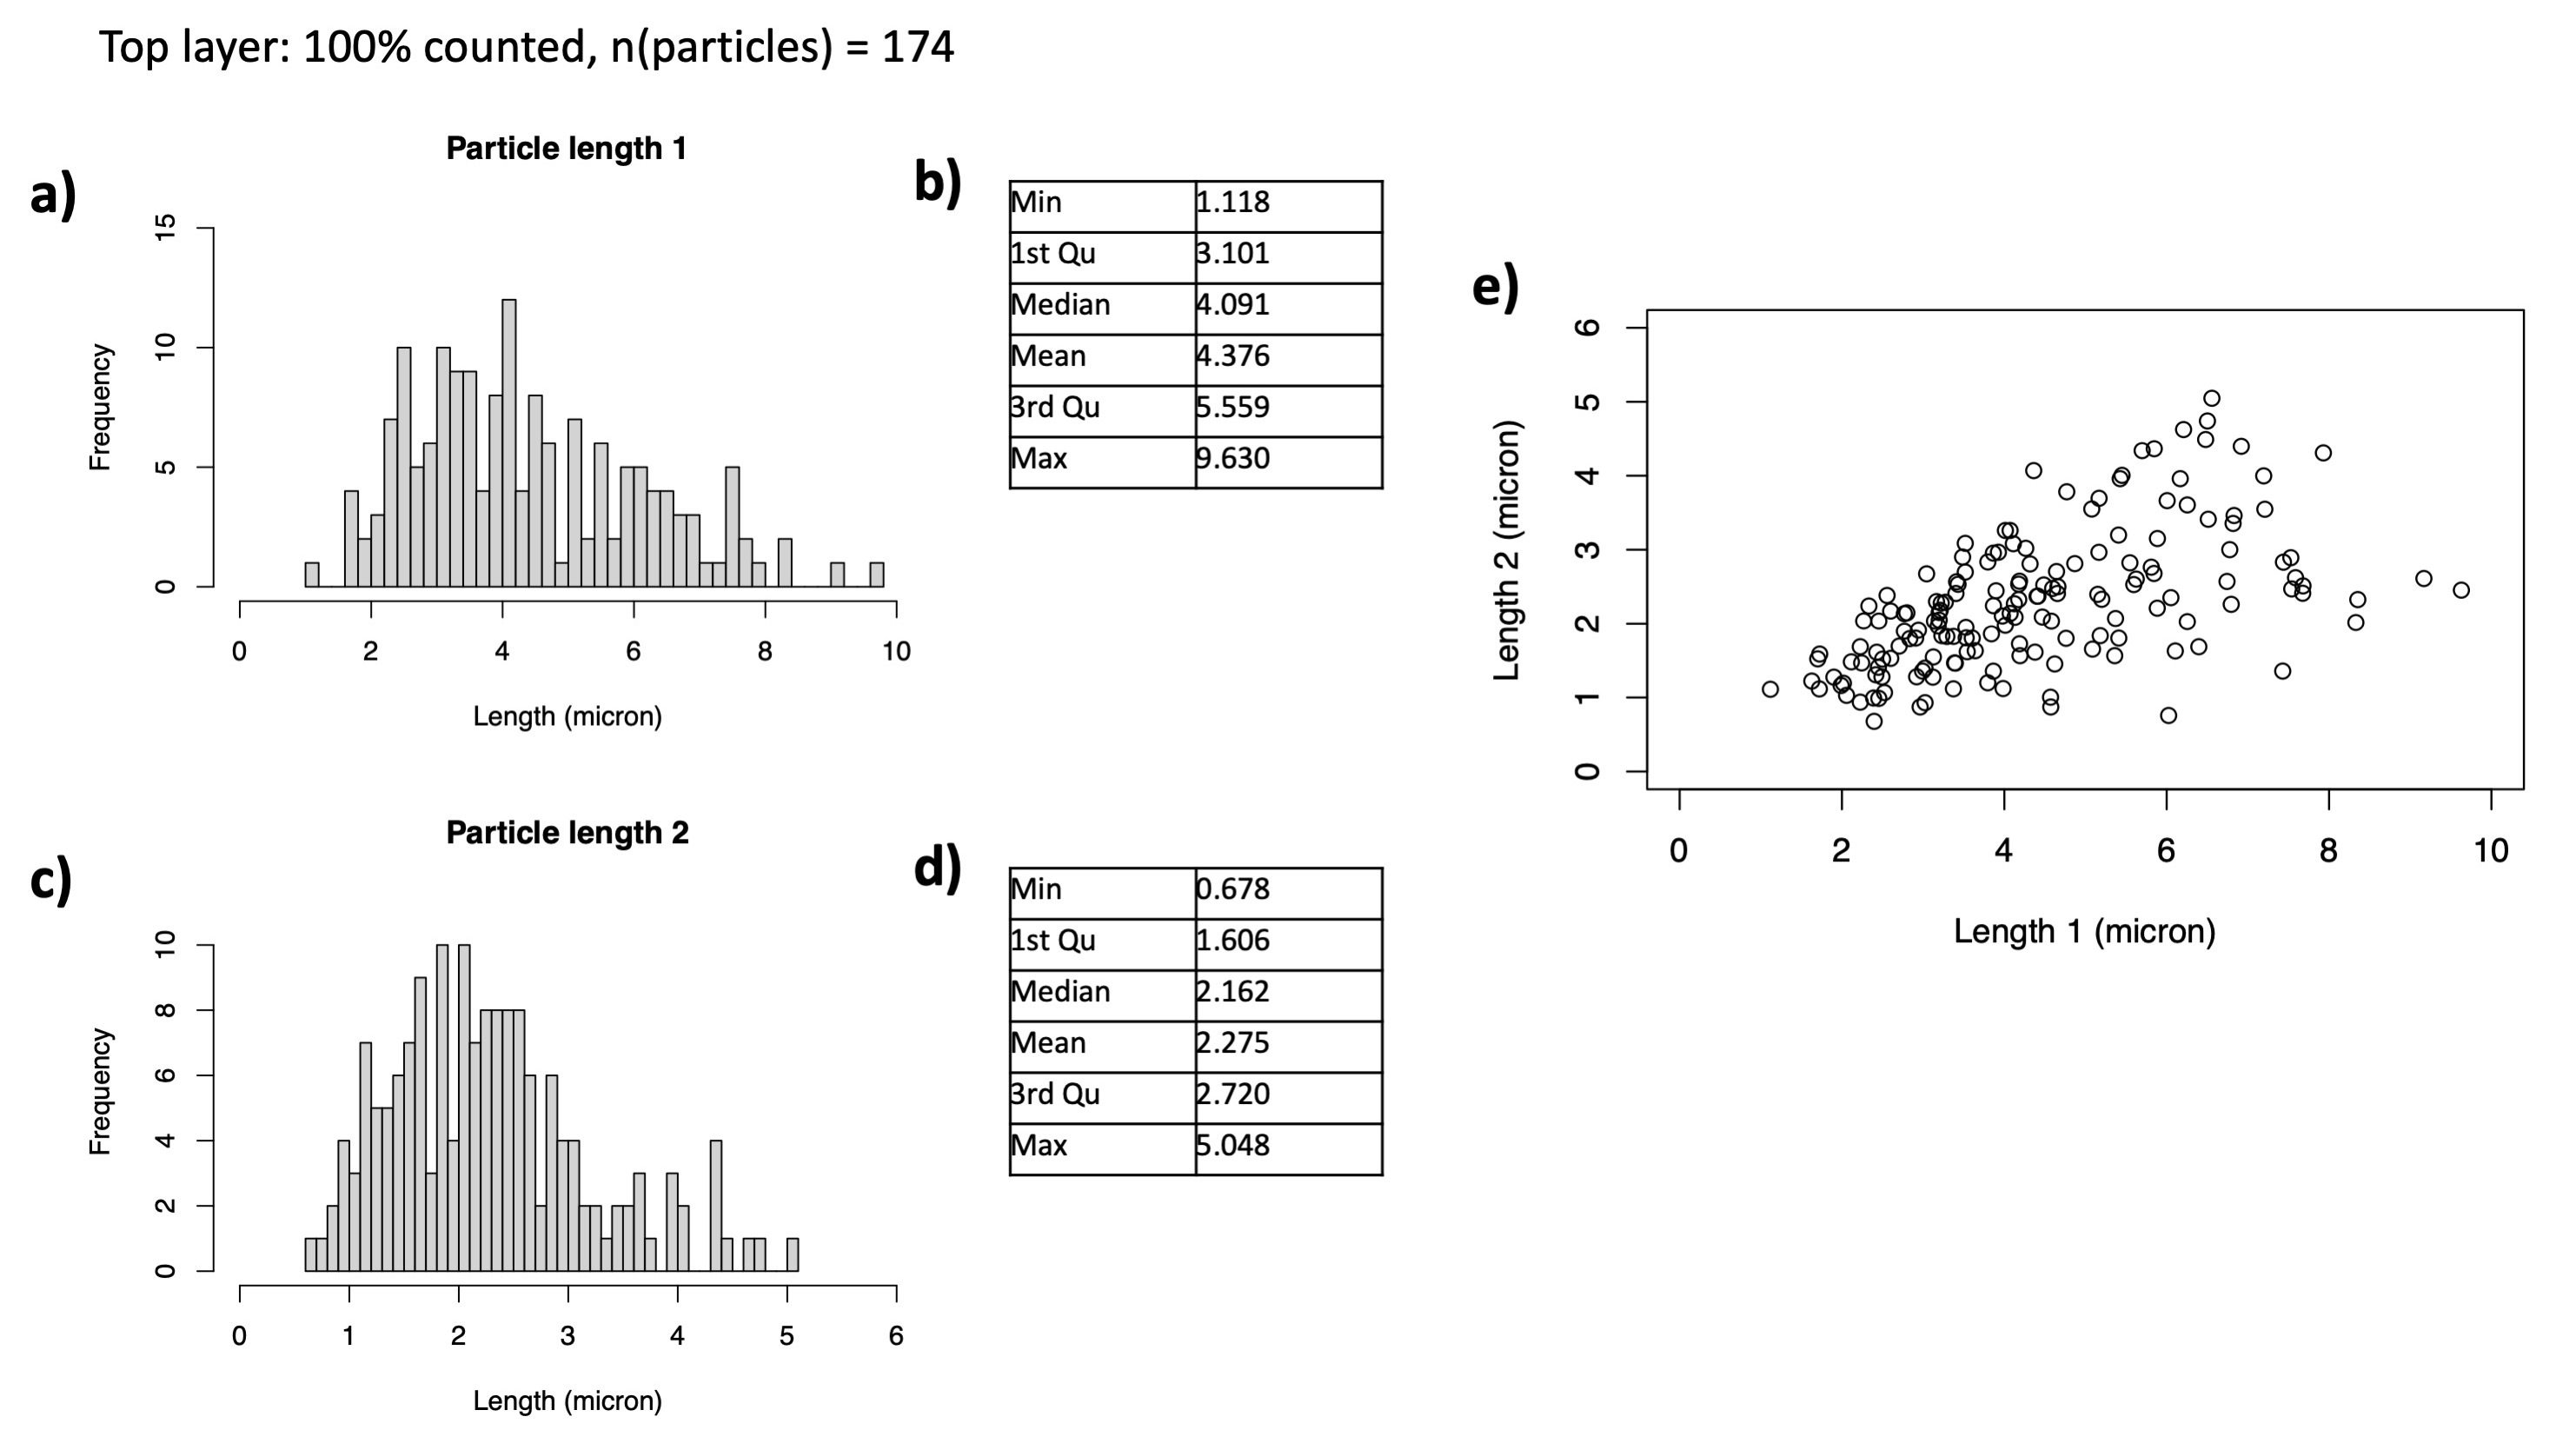
\includegraphics[width=\linewidth]{1259-34_partsize}
\caption[Particle size distribution, sample 1259.34, top layer.]{Particle size distribution of sample 1259.34, top layer: \textbf{a)} Histogram showing distribution of particle length 1 values. \textbf{b)} Descriptive statistics for particle length 1 data. \textbf{c)} Histogram showing distribution of particle length 2 values. \textbf{d)} Descriptive statistics for particle length 2 data. \textbf{e)} Graph of length 1 versus length 2 showing the degree of skew.}
\label{fig:1259.34_partsize_1}
\end{figure}


\section{Sample 1259.49}

\textit{Figures \ref{fig:1259.49_imgs}-\ref{fig:1259.49_partsize}} show SEM and dark field microscope images, EDS maps, and particle size statistics for 1259.49. Imaging of the sample suggests relatively impure azurite pigments, with many inclusions. Mapping data shows azurite as well as aluminosilicates, a small number of iron-based particles, a titanium compound that is likely rutile, and a compound containing lead, sulfur, and arsenic, likely galena. Statistical analysis of particle size/shape shows small particles that are fairly uniform (few outliers) and round rather than skewed.

\begin{figure}[H]
  \centering
  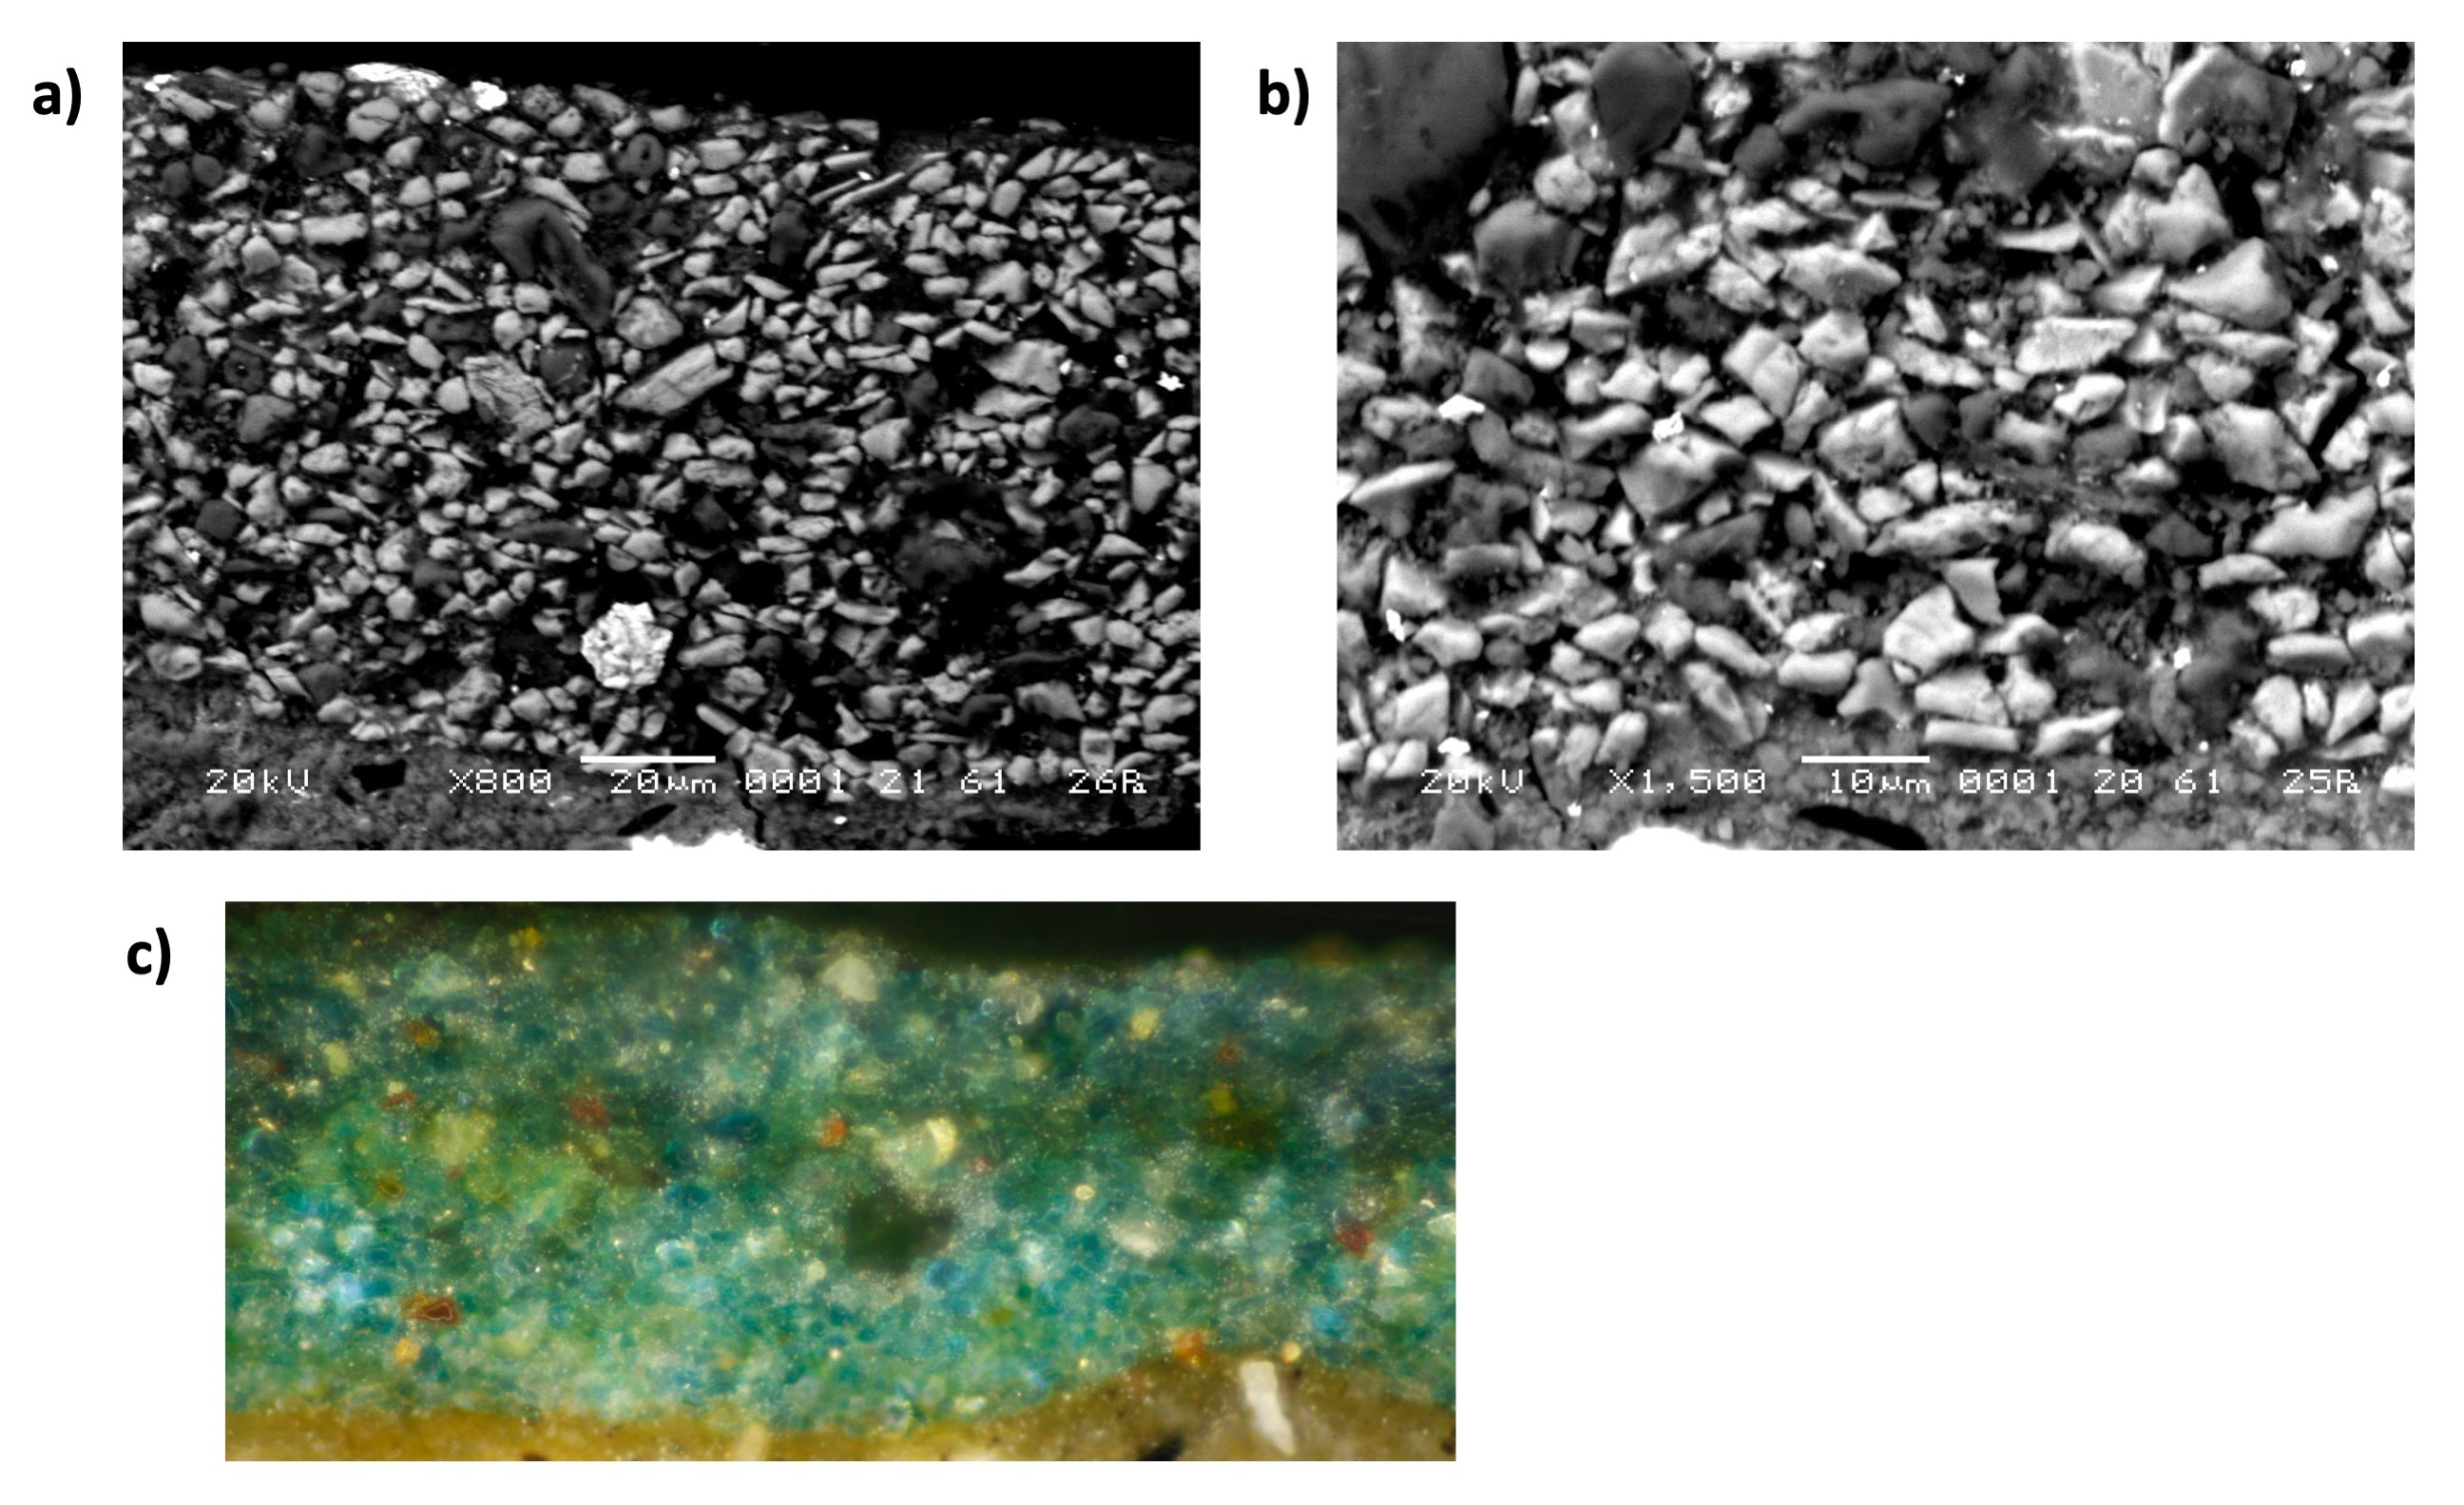
\includegraphics[width=\linewidth]{1259-49_imgs}
\caption[SEM and dark field microscope images of sample 1259.49.]{SEM and dark field microscope images of sample 1259.49: \textbf{a)} 800x magnification, \textbf{b)} 1500x magnification, \textbf{c)} dark field microscope image of sample. Dark field microscope images courtesy of Katharine Waldron, HKI.}
\label{fig:1259.49_imgs}
\end{figure}

\begin{figure}[H]
\centering
\begin{minipage}[t]{\linewidth}
  \centering
  \includegraphics[width=0.9\linewidth]{1259-49_mapdata_1}
\hfill
\includegraphics[width=0.9\linewidth]{1259-49_mapdata_2}
\hfill
\includegraphics[width=0.9\linewidth]{1259-49_mapdata_3}
\hfill
\end{minipage}
\caption[EDS map data, sample 1259.49.]{EDS map data of sample 1259.49 showing locations of elements in an area of the azurite paint layer. Elements detected are Ca, K, S, Zn, Al, Cu, Fe, Ti, Pb, As, Si, and P.}
\label{fig:1259.49_mapdata}
\end{figure}


\begin{figure}[H]
\centering
  \includegraphics[width=\linewidth]{1259-49_partsize}
\caption[Particle size distribution, sample 1259.49.]{Particle size distribution of sample 1259.49: \textbf{a)} Histogram showing distribution of particle length 1 values. \textbf{b)} Descriptive statistics for particle length 1 data. \textbf{c)} Histogram showing distribution of particle length 2 values. \textbf{d)} Descriptive statistics for particle length 2 data. \textbf{e)} Graph of length 1 versus length 2 showing the degree of skew.}
\label{fig:1259.49_partsize}
\end{figure}

\section{Summary of results}

By studying a number of cross sections from the same work, useful information about common associate minerals of azurite as well as statistics about particle size and shape are discovered. 

While some compounds identified, such as vermilion (HgS) and smalt, were likely intentionally mixed with azurite by the artist, others are reasonable associate minerals.~\autocite{Aru} \textit{Table \ref{table:elem_summary_bos}} summarises the frequency of compounds detected by EDS mapping. Dolomite, iron oxides, and aluminosilicates occur frequently, while other associate minerals are less frequently identified. Given the frequency with which multiple associates were identified within the same sample area, it is reasonable to conclude that \textbf{1)} historical pigment preparation methods did not produce especially pure azurite and \textbf{2)} detection of multiple associate minerals is highly indicative of natural pigment.

\begin{table}[H]
\caption{Identified compounds in \textit{Battle of Spurs} azurite pigment layers}
\centering
\label{table:elem_summary_bos}
\begin{tabular}{c c c c}
\toprule
\multicolumn{2}{c} {Compound} & Likely source & Frequency \\
\midrule
\multicolumn{2}{c} {Iron oxide} & associate & 7 \\
\multicolumn{2}{c} {Dolomite} & associate & 6 \\
\multicolumn{2}{c} {Aluminosilicate} & associate & 5 \\
~ & Feldspar & associate & 2 \\
~ & Mg-containing & associate & 1 \\
\multicolumn{2}{c} {Lead (often with arsenic)} & associate, pigment & 5 \\
\multicolumn{2}{c} {Quartz} & associate & 4 \\
\multicolumn{2}{c} {Rutil} & associate & 4 \\
\multicolumn{2}{c} {Calcite} & associate & 2 \\
\multicolumn{2}{c} {Calcium phosphate} & associate & 2 \\
\multicolumn{2}{c} {Silicon-based} & associate & 2 \\
\multicolumn{2}{c} {Aluminium oxide} & associate & 1 \\
\multicolumn{2}{c} {Galena} & associate & 1 \\
\multicolumn{2}{c} {Vermilion} & pigment & 1 \\
\multicolumn{2}{c} {Lead, tin} & unknown & 1 \\
\multicolumn{2}{c} {Potassium-based} & associate & 1 \\
\bottomrule
\end{tabular}
\end{table}

\textit{Table \ref{table:stat_summary_bos}} summarises the statistical data on particle size and shape. Every set of length data showed larger mean values than medians, indicating one or a few outlier large particles. 1259.19, 1259.20, 1259.21, 1259.23, and 1259.34 had extremely large range values and large mean-median variation, while 1259.29 showed a large range and small mean-median variation. This specifically is interesting as it suggests that this sample had a wider spread of length values rather than a small number of outliers. The upper azurite layers of 1259.33 and 1259.34 showed smaller average pigment lengths and small ranges, indicating consistently ground fine pigment. This analysis, while not conclusive, does suggest that it is possible to group pigment layers by pigment size; while most data is similar excepting a few outliers, 1259.29 on one hand and the upper azurite layers of 1259.33 and 1259.34 on the other are significantly different. These may have been from a different batch or prepared by a different method.

\begin{table}[H]
\caption{Particle size statistics, \textit{Battle of Spurs}}
\centering
\label{table:stat_summary_bos}
\begin{tabular}{c c c c c c c}
\toprule
Sample & Dimension & Minimum ($\mu$m) & Maximum ($\mu$m) & Mean ($\mu$m) & Range ($\mu$m) & Mean - median ($\mu$m) \\
\midrule
1259.1 & Length 1 & 1.243 & 12.229 & 5.051 & 10.986 & 0.189 \\
~      & Length 2 & 0.768 & 8.148 & 2.831 & 7.38 & 0.169 \\
1259.6 & 1 & 0.687 & 14.116 & 4.618 & 13.429 & 0.254 \\
~      & 2 & 0.444 & 9.812 & 2.593 & 9.368 & 0.208 \\
1259.14, bottom & 1 & 0.915 & 12.667 & 4.62 & 11.752 & 0.182 \\
~      & 2 & 0.457 & 8.365 & 2.42 & 7.908 & 0.124 \\
1259.14, bottom and top & 1 & 1.214 & 12.871 & 4.648 & 11.657 & 0.143 \\
~      & 2 & 0.657 & 7.006 & 2.562 & 6.349 & 0.129 \\
1259.19 & 1 & 1.04 & 21.151 & 4.491 & 20.111 & 0.445 \\
~       & 2 & 0.488 & 9.683 & 2.276 & 9.195 & 0.197 \\
1259.20 & 1 & 0.82 & 20.15 & 3.736 & 19.33 & 0.468 \\
~       & 2 & 0.403 & 11.969 & 1.92 & 11.566 & 0.269 \\
1259.21 & 1 & 1.49 & 24.253 & 4.938 & 22.763 & 0.477 \\
~       & 2 & 0.718 & 18.1 & 2.632 & 17.382 & 0.235 \\
1259.23 & 1 & 1.864 & 17.857 & 5.341 & 15.993 & 0.616 \\
~       & 2 & 0.658 & 9.599 & 2.875 & 8.941 & 0.124 \\
1259.28 & 1 & 1.109 & 12.349 & 4.299 & 11.24 & 0.4 \\
~       & 2 & 0.658 & 7.747 & 2.444 & 7.089 & 0.174 \\
1259.29 & 1 & 0.992 & 19.342 & 4.515 & 18.35 & 0.114 \\
~       & 2 & 0.671 & 15.257 & 2.472 & 14.586 & 0.243 \\
1259.33, bottom & 1 & 1.152 & 13.001 & 4.149 & 11.849 & 0.37 \\
~       & 2 & 0.625 & 7.603 & 2.249 & 6.978 & 0.154 \\
1259.33, top & 1 & 1.132 & 9.757 & 3.89 & 8.625 & 0.263 \\
~       & 2 & 0.5 & 7.234 & 2.113 & 6.734 & 0.186 \\
1259.34, bottom & 1 & 0.756 & 17.772 & 4.509 & 17.016 & 0.462 \\
~       & 2 & 0.576 & 7.093 & 2.337 & 6.517 & 0.114 \\
1259.34, top & 1 & .118 & 9.63 & 4.376 & 8.512 & 0.285 \\
~       & 2 & 0.678 & 5.048 & 2.275 & 4.37 & 0.113t \\
1259.49 & 1 & 0.701 & 12.932 & 4.896 & 12.231 & 0.304 \\
~       & 2 & 0.422 & 9.045 & 2.611 & 8.623 & 0.178 \\
\bottomrule
\end{tabular}
\end{table}



%Routes of analysis, research questions
%. Will be proceeding with collaborative project with HKI on analysis of wall painting samples containing blue pigments using the analytic methods outlined in this report. The discussed parameters, specifically particle morphology, size distribution, trace element analysis: have shown to be able to be characterized using the combination of analytic methods used here. Additional analysis may involve mass spec (add more specifics) as needed.

%Additional samples of natural azurite (geologic formations) and easel painting cross sections containing both natural azurite and synthetic blue verditer pigments will be added to develope a more complete library of statistically relevant variation in samples depending on natural or synthetic origins.

%2. Analysis of pigment preparation (size/shape distribution) in HKI cross section samples taken from easel paintings and samples prepared using historic grinding and purification procedures in the laboratory: collaborative work with HKI, entailing analysis of particle morphology and size distribution using SEM-EDS and AFM-IR to 1) confirm pigment identifications and 2) characterize a range of samples accoridng to pigment size distributions and morphological variation. Some analysis of pigment behaviour in binder depending on size may also be added.

%3. Potential interesting questions remain and may be addressed further into the project. These include attaining a better understanding of the optical effects of pigment size and shape as well as potentially binder interactions which could also affect the reflective index of the paint layer containing azurite particles. These also include a discussion of provenancing of natural azurite, as this work has been limited in the past due to sample sizes available. This will build on existing literature concerning pigment mineral provenancing that has primarily focussed on lapis lazuli (ultramarine) and cinnabar (vermilion). 

%Samples: 
%Highly collaborative project. 1. Will be acquiring a range of samples from HKI, from existing collections (Andrea Kirkham), from potentially visits to building sites (obiously not discussed ATM due to covid), and from the Sedgwick Museum of Earth Sciences. 

